\documentclass[a4paper, twoside]{book}
\usepackage[T1]{fontenc}
\usepackage[utf8]{inputenc}
\usepackage[italian]{babel}
\usepackage{amsmath, amssymb, amsthm}
\usepackage{geometry}
\usepackage{titling}
\usepackage{enumitem}
\usepackage{pdfpages}
\usepackage{graphicx, float}
\usepackage{subcaption}
\usepackage{caption}
\usepackage{hyperref}
\usepackage{mdframed} % Pacchetto per le cornici
\usepackage{xcolor}   % Pacchetto per la gestione dei colori
\usepackage{forest} %diagrammi ad albero

% Colore per il background delle cornici
\definecolor{grey245}{RGB}{245,245,245}

% Teoremi e definizioni
\theoremstyle{plain}
\newtheorem{theorem}{\textsc{Teorema}}[chapter] 
\newtheorem{lemma}[theorem]{\textsc{Lemma}}
\newtheorem{corollary}[theorem]{\textsc{Corollario}}
\newtheorem{proposition}[theorem]{\textsc{Proposizione}}

\theoremstyle{definition}
\newtheorem{definition}{\textsc{Definizione}}[chapter]  
\newtheorem{example}{\textsc{Esempio}}[chapter] 


%Cornice teorema
\newmdenv[skipabove=5pt,
skipbelow=5pt,
rightline=false,
leftline=true,
topline=false,
bottomline=false,
linecolor=purple,
backgroundcolor=purple!0,
innerleftmargin=5pt,
innerrightmargin=5pt,
innertopmargin=0pt,
innerbottommargin=2pt,
leftmargin=0cm,
rightmargin=0cm,
linewidth=2pt,
splitbottomskip=0pt]{theoremBox}


%Cornice definizione
\newmdenv[skipabove=5pt,
skipbelow=5pt,
rightline=false,
leftline=true,
topline=false,
bottomline=false,
linecolor=blue,
backgroundcolor=blue!0,
innerleftmargin=5pt,
innerrightmargin=5pt,
innertopmargin=0pt,
leftmargin=0cm,
rightmargin=0cm,
linewidth=2pt,
innerbottommargin=2pt]{definitionBox}

%Cornice proposizione
\newmdenv[skipabove=5pt,
skipbelow=5pt,
rightline=false,
leftline=true,
topline=false,
bottomline=false,
linecolor=teal,
backgroundcolor=teal!0,
innerleftmargin=5pt,
innerrightmargin=5pt,
innertopmargin=0pt,
leftmargin=0cm,
rightmargin=0cm,
linewidth=2pt,
innerbottommargin=2pt]{propositionBox}

%Cornice lemma
\newmdenv[skipabove=5pt,
skipbelow=5pt,
rightline=false,
leftline=true,
topline=false,
bottomline=false,
linecolor=orange,
backgroundcolor=orange!0,
innerleftmargin=5pt,
innerrightmargin=5pt,
innertopmargin=0pt,
leftmargin=0cm,
rightmargin=0cm,
linewidth=2pt,
innerbottommargin=2pt]{lemmaBox}

%Cornice corollario
\newmdenv[skipabove=5pt,
skipbelow=5pt,
rightline=false,
leftline=true,
topline=false,
bottomline=false,
linecolor=green,
backgroundcolor=green!0,
innerleftmargin=5pt,
innerrightmargin=5pt,
innertopmargin=0pt,
leftmargin=0cm,
rightmargin=0cm,
linewidth=2pt,
innerbottommargin=2pt]{corollaryBox}


% Definizione degli ambienti con cornici senza cambiare i nomi
\let\oldtheorem\theorem
\renewenvironment{theorem}{\begin{theoremBox}\oldtheorem}{\end{theoremBox}}
\let\oldlemma\lemma
\renewenvironment{lemma}{\begin{lemmaBox}\oldlemma}{\end{lemmaBox}}
\let\oldcorollary\corollary
\renewenvironment{corollary}{\begin{corollaryBox}\oldcorollary}{\end{corollaryBox}}
\let\oldproposition\proposition
\renewenvironment{proposition}{\begin{propositionBox}\oldproposition}{\end{propositionBox}}
\let\olddefinition\definition
\renewenvironment{definition}{\begin{definitionBox}\olddefinition}{\end{definitionBox}}

% Ambiente per osservazioni
\newenvironment{oss}
{\par\indent\small{\textbf{Osservazione}}}
{\par}

\newcommand{\subtitle}[1]{%
  \posttitle{%
    \par\end{center}
    \begin{center}\large#1\end{center}
    \vskip0.5em}%
}
%Scorciatoie:
\newcommand{\R}{\mathbb{R}}
\newcommand{\N}{\mathbb{N}}
\newcommand{\U}{\mathcal{U}}
\newcommand{\ppartial}{\partial^+}
\newcommand{\fn}{f_n}
\newcommand{\sn}{s_n}

%Nuovi operatori matematici
\DeclareMathOperator{\Div}{div}
\DeclareMathOperator{\Grad}{grad}
\DeclareMathOperator{\Rot}{rot}
\DeclareMathOperator{\area}{Area}
\DeclareMathOperator{\rank}{rank}
\DeclareMathOperator{\Span}{Span}

%Arraystretch per spaziare le righe tra le matrici
   \renewcommand{\arraystretch}{1.25}

\begin{document}
\frontmatter
\pagestyle{empty}
\newgeometry{left=0cm, right=0cm, top=0cm, bottom=0cm}
\vspace*{\fill}
\begin{center}
	{\large \textsc{Appunti di}}\\
	\vspace*{0.4cm}
	{\Huge \textsc{Analisi Matematica 2}}\\
	\vspace*{0.6cm}
	{\large per il corso di Ingegneria Matematica}\\
	\vspace*{0.4cm}
	{\large {di Pietro Ferrario}}\\
	\vspace*{1cm}
	Politecnico di Milano\\
	A.A. 2024/2025
\end{center}
\vspace*{\fill}
\restoregeometry
\cleardoublepage
\vspace*{\stretch{10}}
\textcopyright \ L'autore, alcuni diritti riservati.\\
\vspace*{6pt}

\textbf{Disclaimer:} Questo libro raccoglie gli appunti del corso di \emph{Analisi Matematica 2} per ingegneri matematici tenuto al Politecnico di Milano nell'anno accademico 2024-2025. I docenti di riferimento sono il Professor Maurizio Garrione e l'esercitatore Norman Potrich.
Il testo di riferimento è:

N. Fusco, P. Marcellini, C. Sbordone, \textit{Lezioni di Analisi matematica due}, Editore: Zanichelli, Anno edizione: 2020


Si sottolinea che i docenti sopracitati non hanno revisionato l'opera e che essa è stata fatta da studenti per studenti, senza alcuna pretesa di sostituire un libro di testo.
\vspace*{12pt}

L'opera è rilasciata sotto la licenza CC BY-NC-SA 4.0, consultabile al sito:\\
\url{https://creativecommons.org/licenses/by-nc-sa/4.0/}
\newline
In sintesi è possibile condividere e modificare il materiale a patto che sia dato il credito adeguato,  fornendo un link alla licenza e indicando eventuali modifiche, e non sia utilizzato a scopi commerciali, come la stampa per la rivendita.\\

\vspace*{\stretch{1}}
\noindent\textsc{Creato il:} \today\\
\noindent\textsc{Sviluppato da:}
\textsc{Pietro Ferrario} - \texttt{pietro4.ferrario@mail.polimi.it}

Per eventuali segnalazioni o miglioramenti è possibile contattare direttamente l'autore o aprire una Pull Request.\clearpage
\tableofcontents
\mainmatter
\pagestyle{plain}
\chapter{Curve}
\section{Curve parametriche}
\begin{definition}
    Si dice \textbf{curva} una funzione continua $\varphi:I\to\mathbb{R}^n$ con $I\subseteq \mathbb{R}$.
\end{definition}
Il parametro di tali funzioni è convenzionalmente $t$. Esse possono essere rappresentate come:
\begin{equation}
    \varphi(t)=(\varphi_1(t), \varphi_2(t), \dots, \varphi_n(t)) \text{ con }\varphi_i:I \to \mathbb{R}
\end{equation}
Analogamente, è possibile utilizzare le \textbf{equazioni parametriche della curva}, cioè:
\begin{equation}
   \begin{cases}
     x_1=\varphi_1(t)\\
     \vdots\\
     x_n=\varphi_n(t)\\
    \end{cases}
\end{equation}
\begin{oss}
    Con \textbf{continua} si intende dire che $\varphi$ sia continua componente per componente, cioè che:
    \begin{equation}
        \varphi \text{ continua in } t_0 \in I \text{ } \iff \text{ } \lim_{t \to t_0}{\varphi_i(t)}=\varphi_i(t_0) \text{ }\forall i=1, \dots, n.
    \end{equation} 
\end{oss}
\begin{oss}
    Sia $l=(l_1, \dots, l_n)\in\mathbb{R}$ e sia $t_0$ un punto di accumulazione per il dominio di $\varphi$. Allora,
    \begin{equation}
        \lim_{t \to t_0}{\varphi(t)}=l \text{ }\iff \text{ }\lim_{t \to t_0}{\varphi_i(t)}=l_i \text{ } \forall i = 1, \dots, n.
    \end{equation}
\end{oss}
\begin{oss}
    Il discorso appena visto vale anche per quanto riguarda la derivabilità di $\varphi$. Infatti $\varphi$ è derivabile in $t_0$ se e solo se $\varphi_i$ è derivabile in $t_0$ $\forall i=1, \dots, n$. Di conseguenza: $\varphi'(t)=(\varphi_1'(t), \dots, \varphi_n'(t))$.
\end{oss}
\begin{definition}
    Si dice \textbf{sostegno della curva} l'immagine $\varphi(I) \subseteq \mathbb{R}^n$.
\end{definition}
\begin{example}
   Si consideri la retta di equazioni $r:\underline{x}_0+t\underline{v}$ con $t \in \mathbb{R}$. Il suo sostegno sarà una retta. Si parametrizzi di seguito un segmento di estremi $x_0, x_1$.\\
   Si trovi $t$ tale che $x_0$ e $x_1$ appartengano ad $r$. Dopodiché si valuti l'intervallo $I$ tale che $\varphi(I)$ sia il sostegno.
   \begin{equation*}
    \begin{aligned}  
        r&=\underline{x}_0 \iff t=0\\
        r&=\underline{x}_1 \iff t\underline{v}+\underline{x}_0=\underline{x_1}\iff t\underline{v}=\underline{x}_1-\underline{x}_0\\
        \text{Dunque,}&\ t|\underline{v}|\underline{u}_v=|\underline{x}_1-\underline{x}_0|\underline{u}_v \iff t=\frac{|\underline{x}_1-\underline{x}_0|}{|\underline{v}|}
    \end{aligned}
    \end{equation*}
    Allora, $\underline{x}_0 + t\underline{v}$ è un segmento di estremi $x_0, x_1$ $\iff t \in \left[0, \frac{|\underline{x}_1-\underline{x}_0|}{|\underline{v}|}\right]$.\\ 
   Un metodo alternativo per la parametrizzazione di tale segmento è l'utilizzo di una combinazione convessa $(1-t) x_0 + tx_1$ con $t \in [0,1]$.
\end{example}
\begin{example}
    Si consideri ora la seguente curva: $\varphi(t)=(R \cos(t), R \sin(t))$. Dipendentemente da $I$ il sostegno è diverso. Infatti:
\begin{figure}[H]
    \centering
    \begin{minipage}{0.25\textwidth}
        \centering
        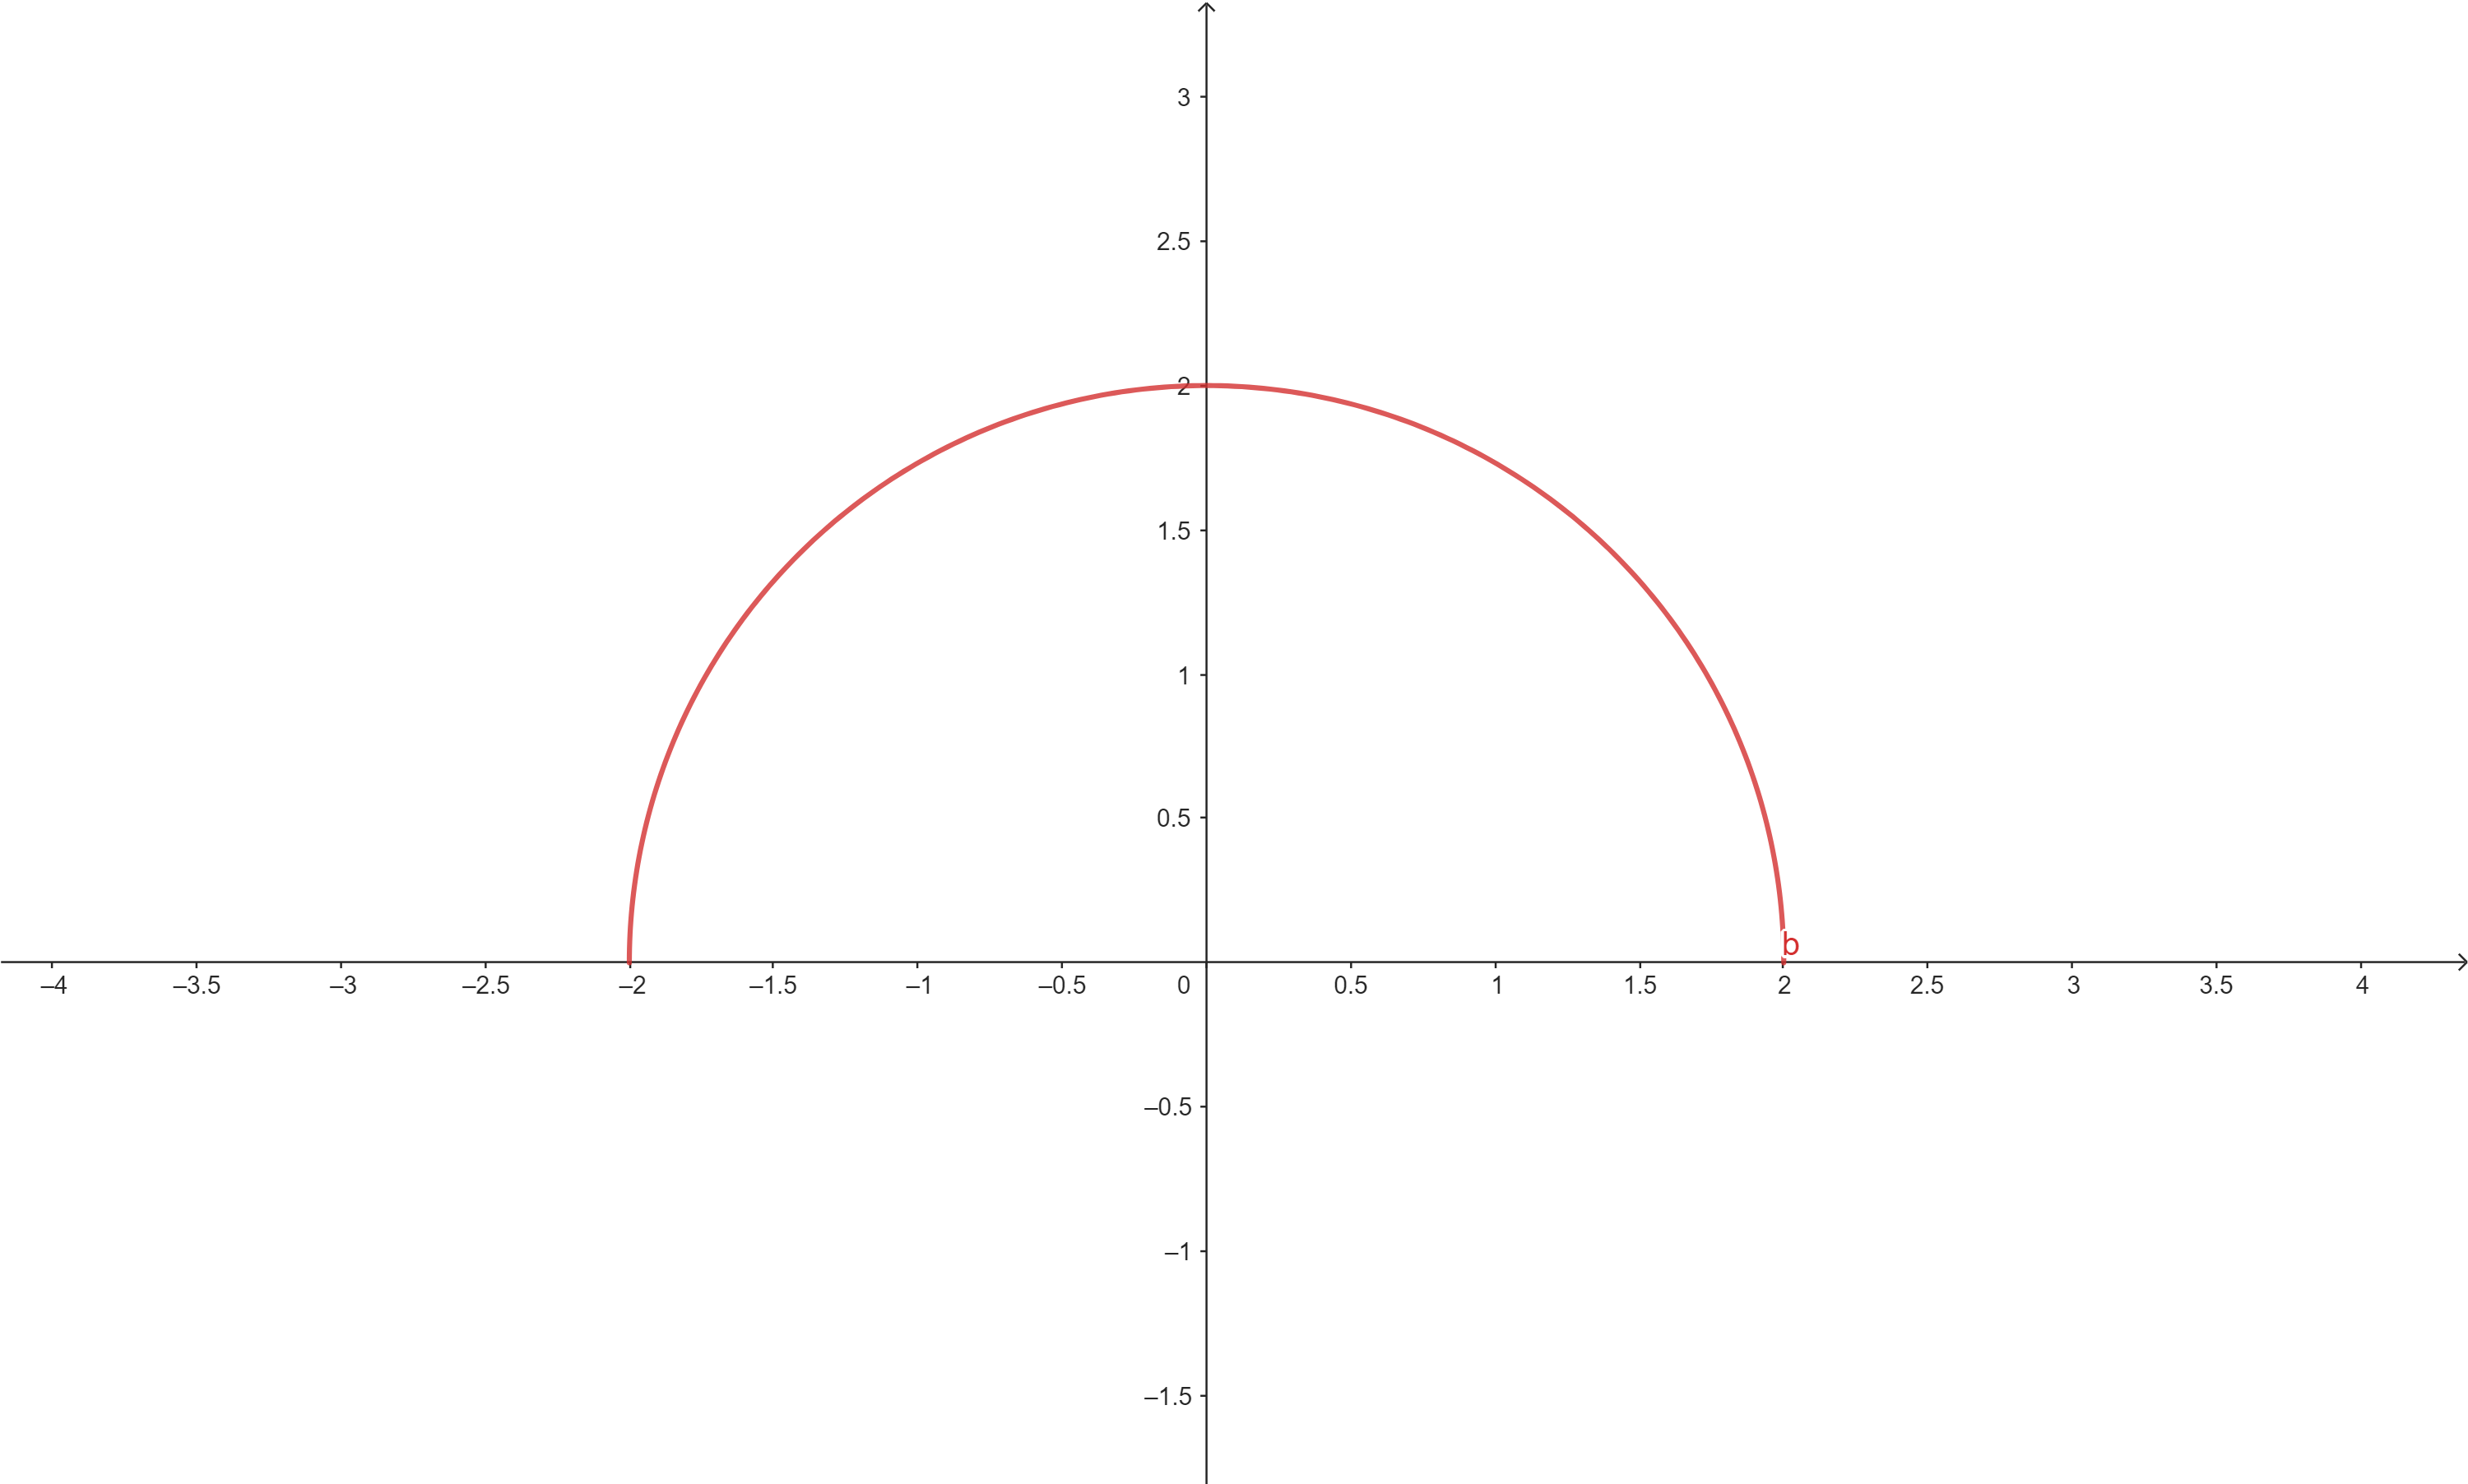
\includegraphics[width=\textwidth]{Capitoli/Capitolo1/sostegno_circ1.png}
        \caption{Sostegno di $\varphi(t)$ con $R=2$ e $t\in[0, \pi]$}
    \end{minipage}
    \hspace{1cm}
    \begin{minipage}{0.25\textwidth}
        \centering
        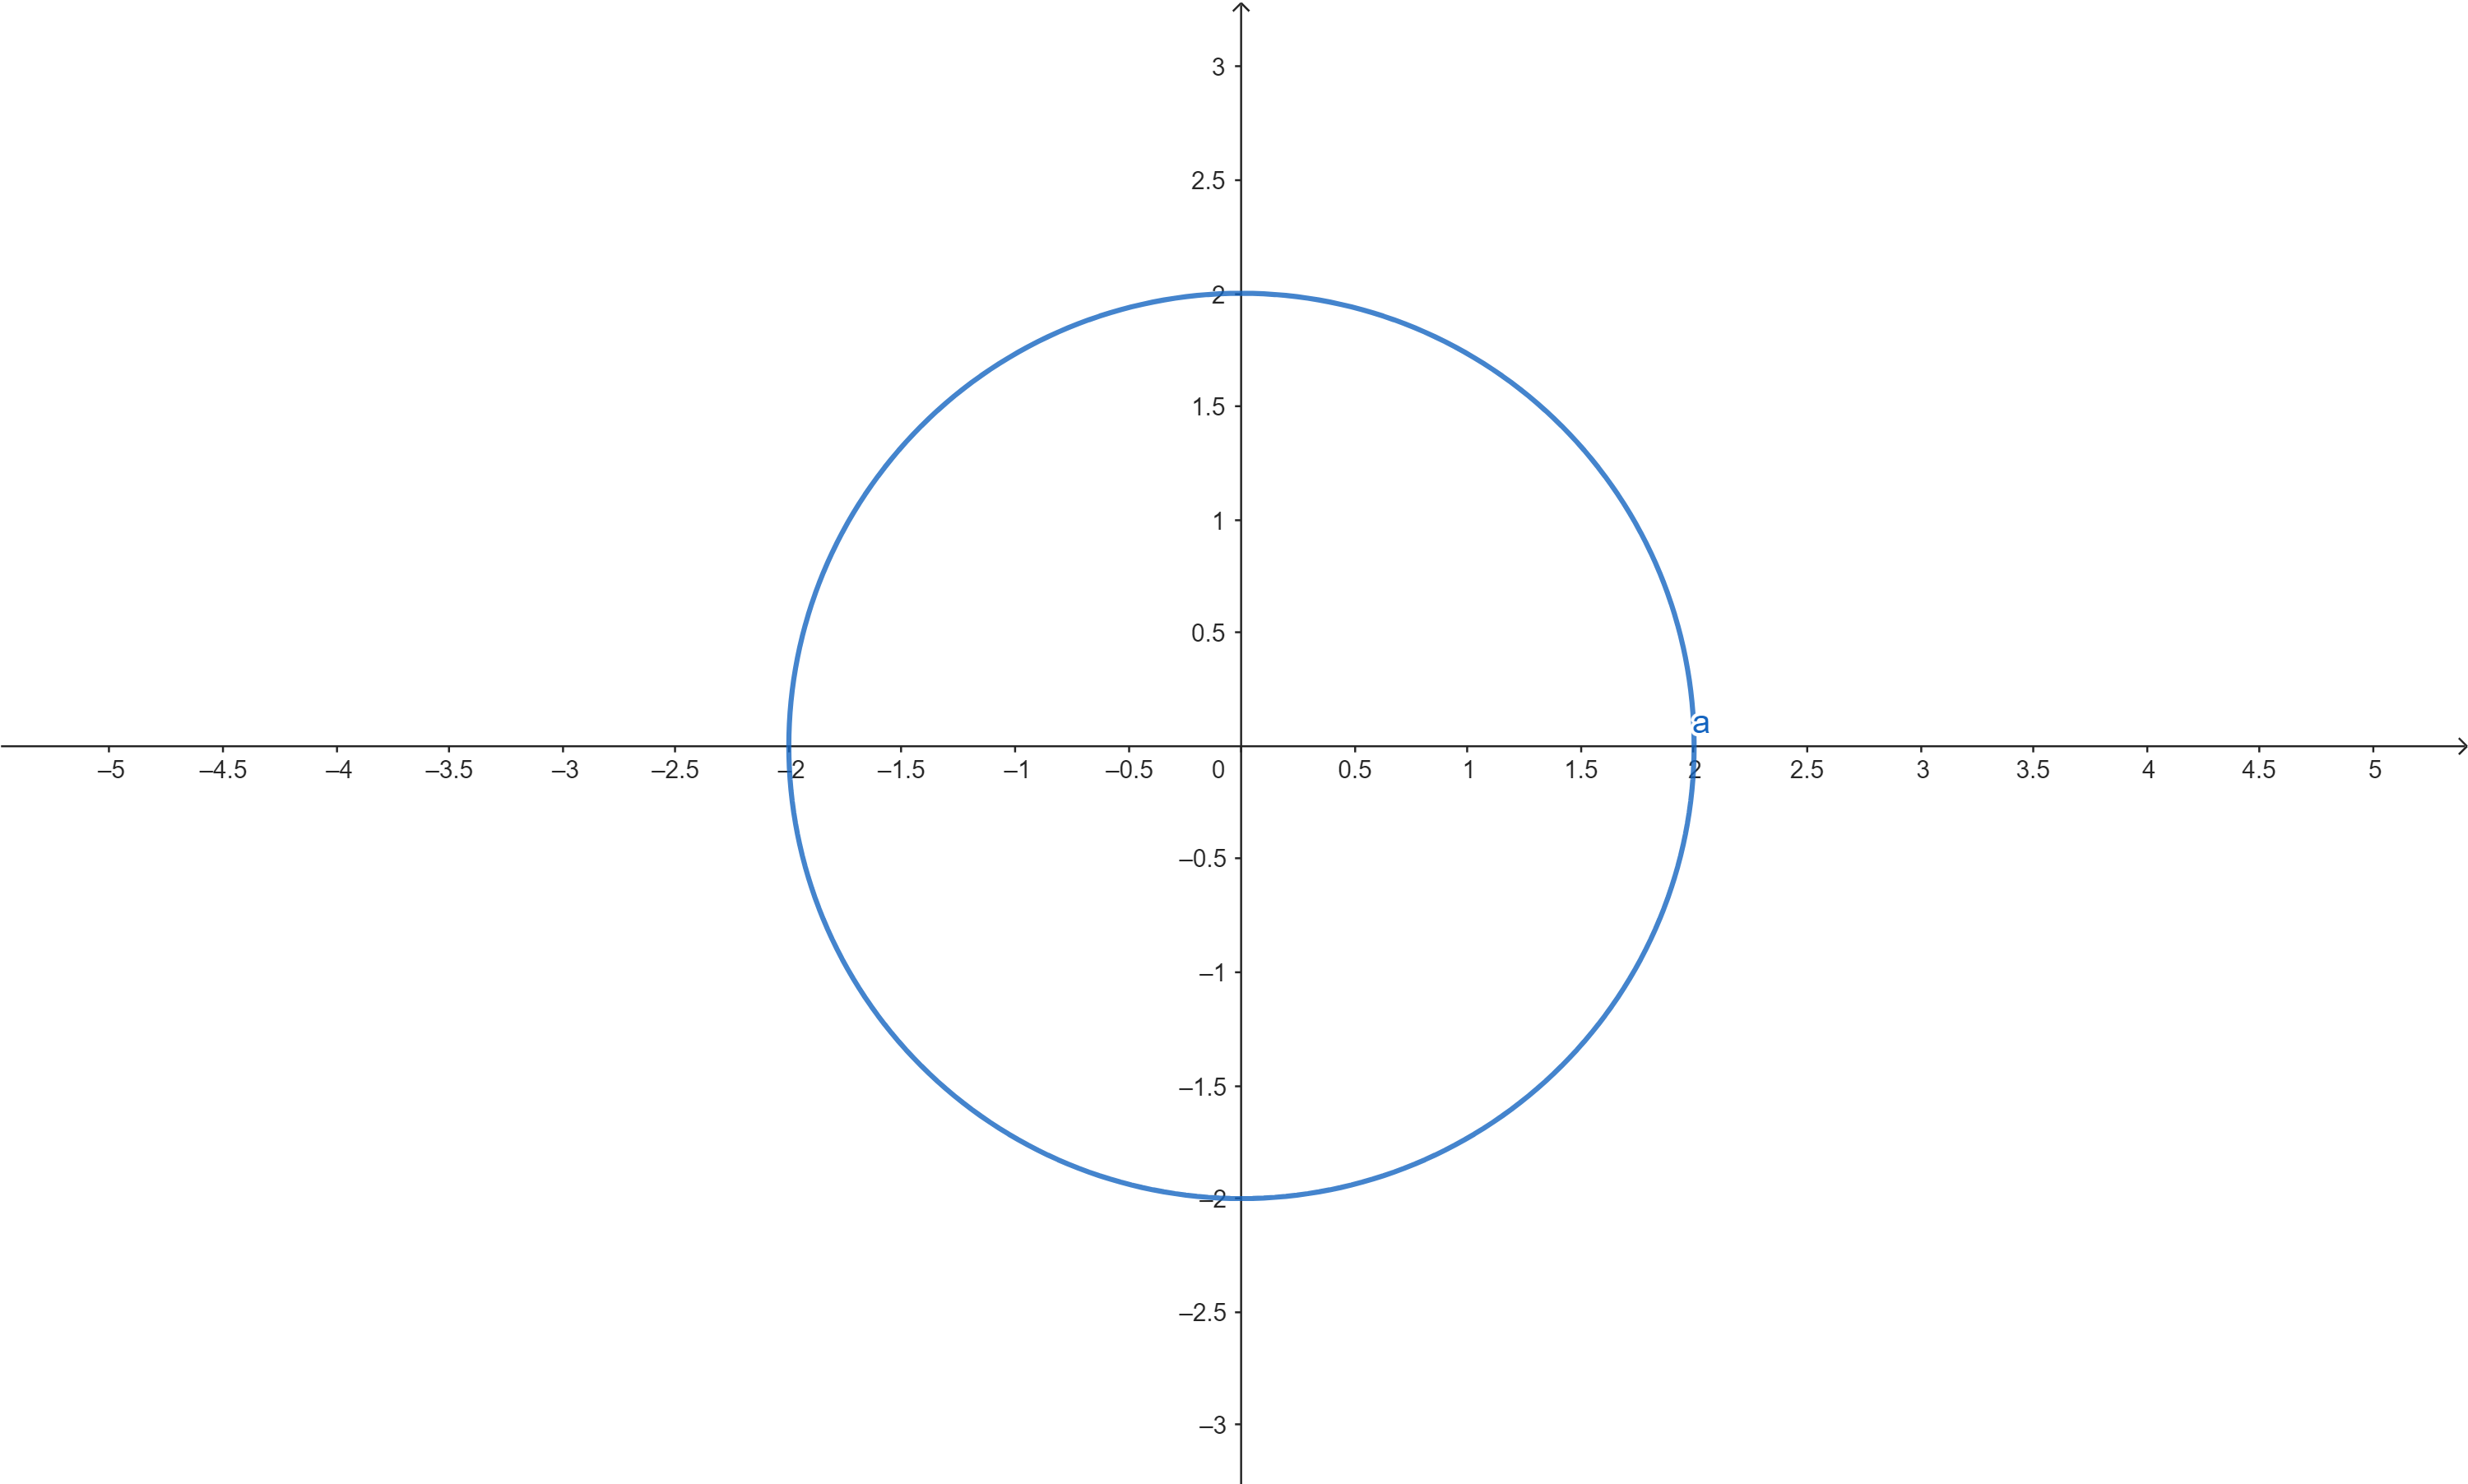
\includegraphics[width=\textwidth]{Capitoli/Capitolo1/sostegno_circ2.png}
        \caption{Sostegno di $\varphi(t)$ con $R=2$ e $t\in[0, 2\pi]$}
    \end{minipage}
    \hspace{1cm}
    \begin{minipage}{0.25\textwidth}
        \centering
        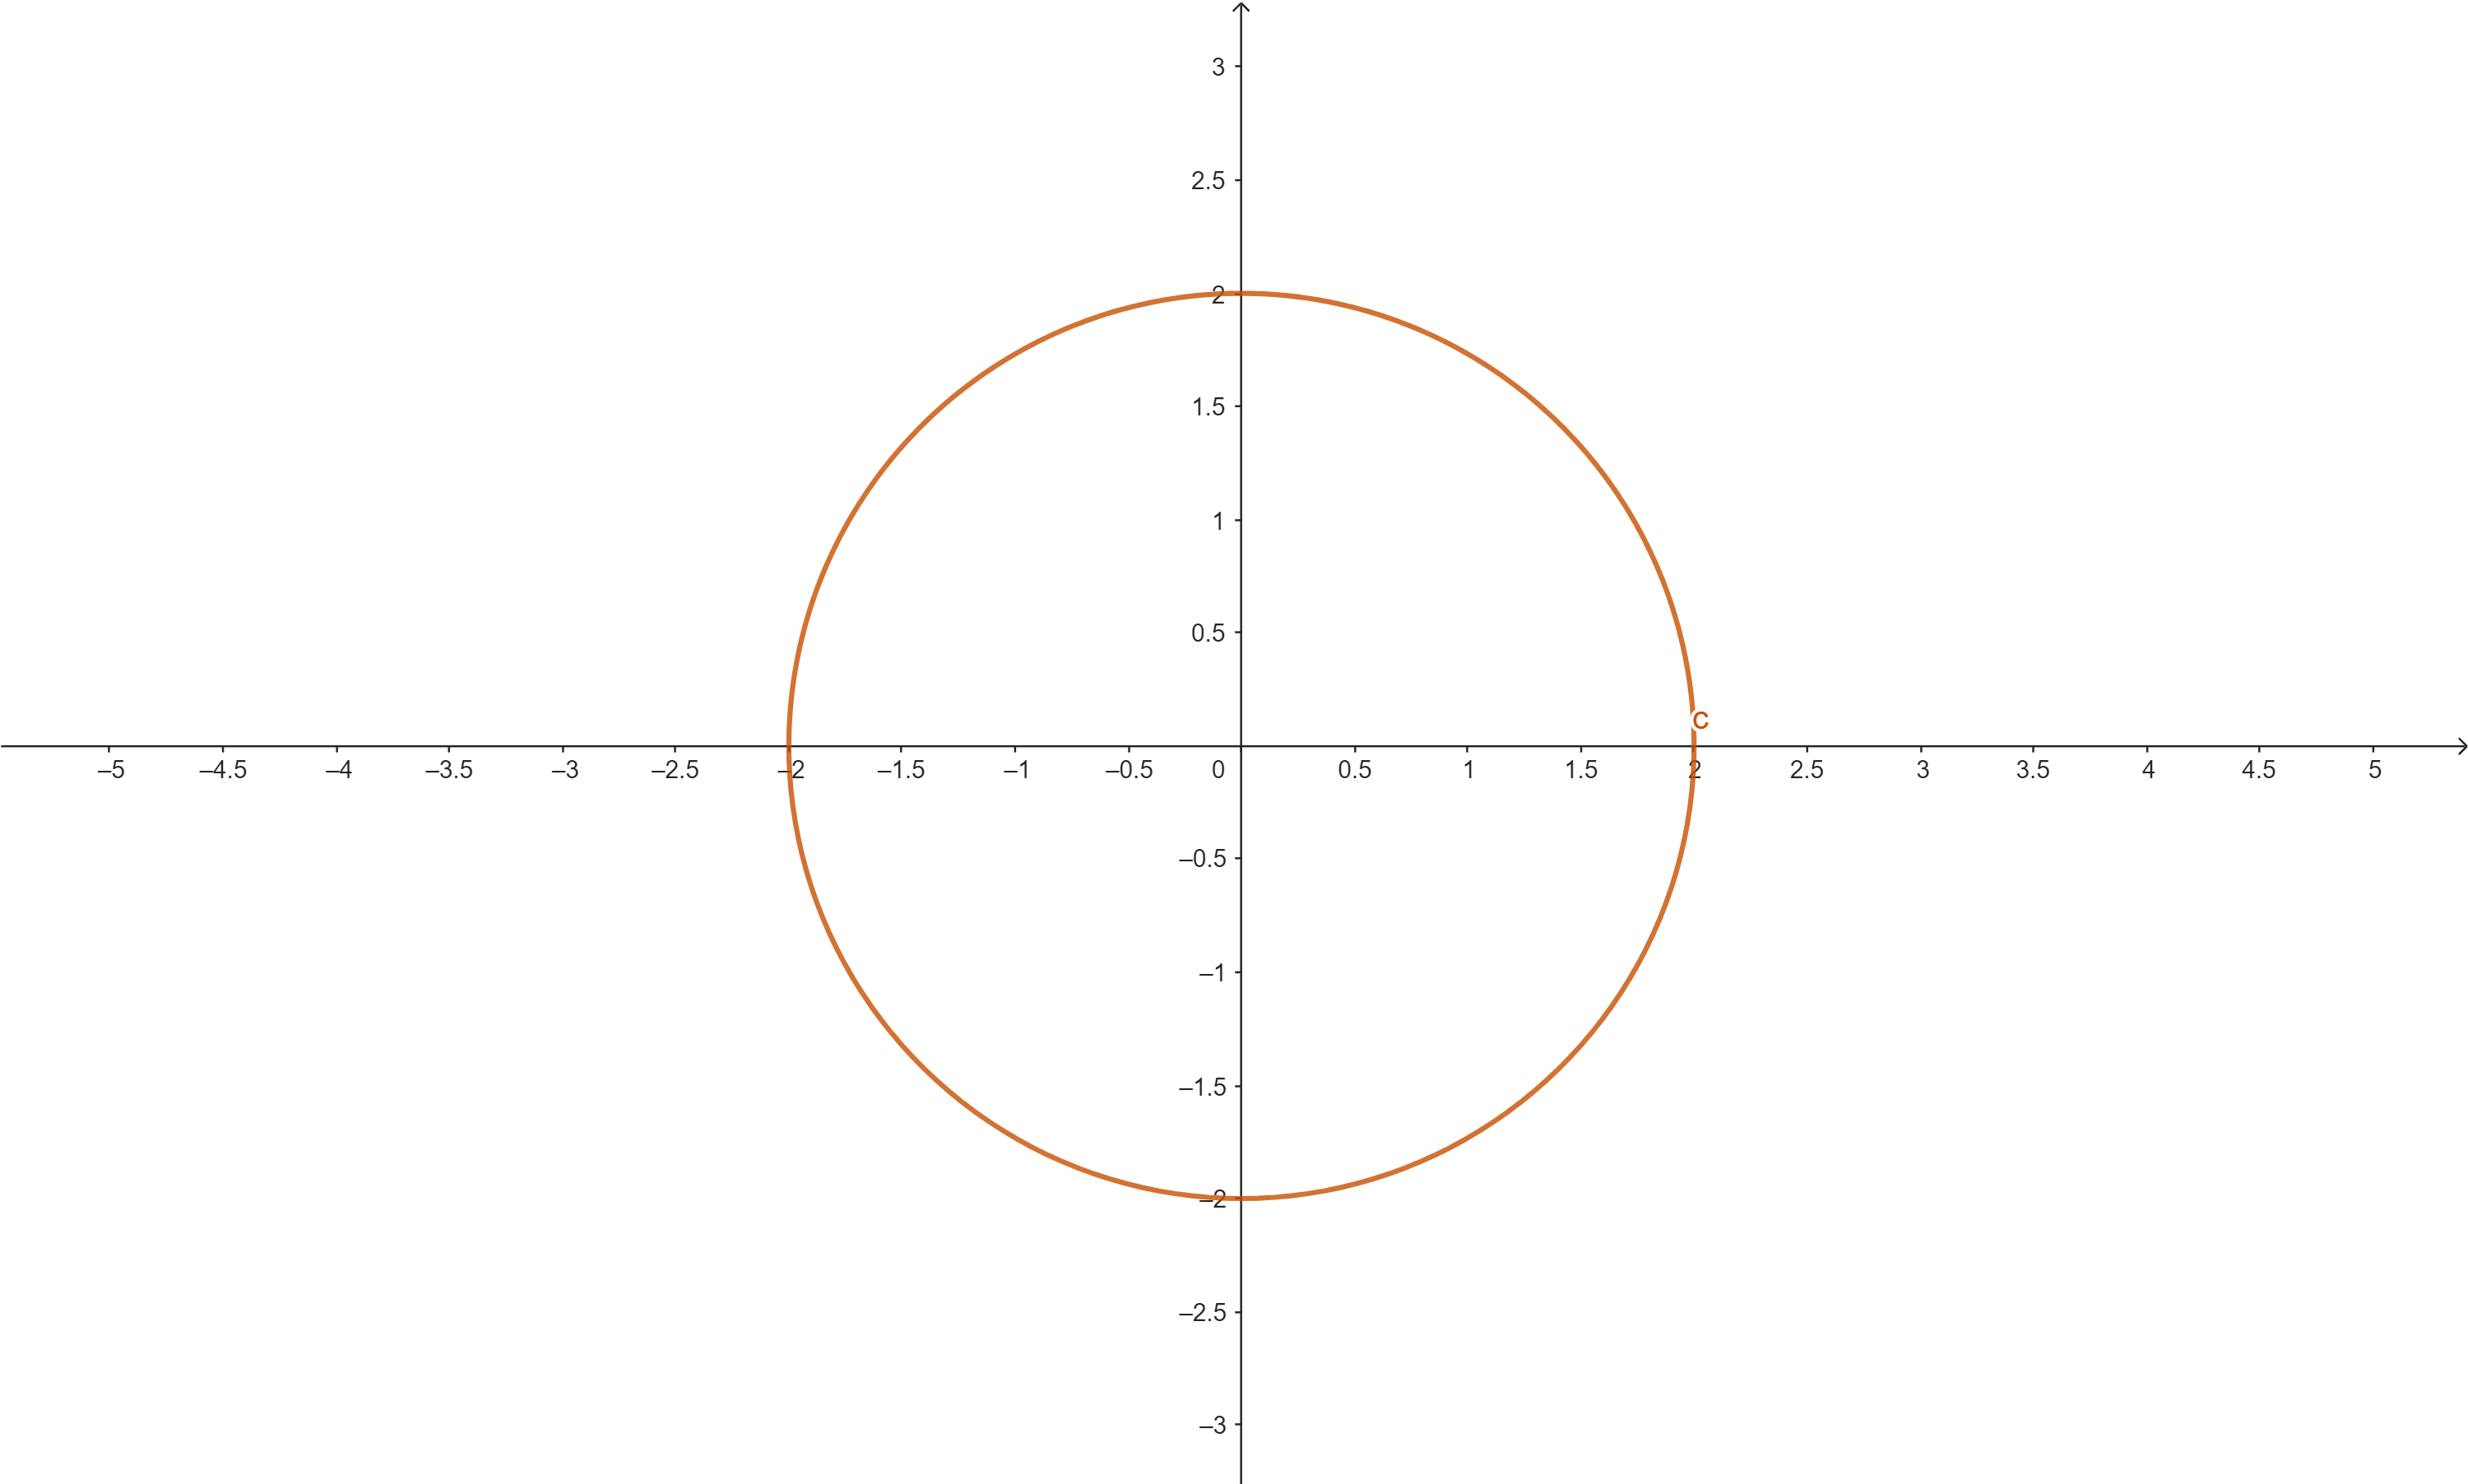
\includegraphics[width=\textwidth]{Capitoli/Capitolo1/sostegno_circ3.png}
        \caption{Sostegno di $\varphi(t)$ con $R=2$ e $t\in[0, 3\pi]$}
    \end{minipage}
\end{figure}
\end{example}
Da ciò si può osservare come, \textit{in primis}, la definizione di $I$ sia fondamentale nel tracciare il sostegno e, \textit{in secundis}, come, d'altra parte, il sostegno non identifichi la curva. A tal proposito infatti occorre notare che, benché le curve associate ai sostegni delle figure 1.2 e 1.3 siano diverse, i loro sostegni sono uguali.
\begin{example}    
    Un'altra casistica è quella rappresentata dalla curva di equazione $\varphi(t)=(R \cos(-t), R \sin(-t))$. Il suo sostegno, infatti, rimane la circonferenza (o l'arco) di raggio $R$, percorso tuttavia in senso orario.
\end{example}
\begin{definition}
    Sia $\varphi:[I \to \mathbb{R}^n]$ una curva parametrica. Allora si dice che $P_1=\varphi(t_1)$ \textbf{precede} $P_2=\varphi(t_2)$ nel verso delle $t$ crescenti se $t_1<t_2$ con $t_1, t_2 \in I$.
\end{definition}
\subsection{Proprietà delle curve parametriche}
Fatte tali premesse, si passi ad analizzare alcune proprietà delle curve.
\begin{definition}
    Una curva $\varphi:[a,b]\to\mathbb{R}^n$ si dice \textbf{chiusa} se $\varphi(a)=\varphi(b)$.
\end{definition}
\begin{oss}
    Si noti a tal proposito che la curva in figura 1.3 non è chiusa, mentre quella in figura 1.2 sì.
\end{oss}
\begin{definition}
    Una curva $\varphi:[a,b] \to \mathbb{R}^n$ si dice \textbf{semplice} se, $\forall$ $ t_1, t_2 \in [a,b]$ distinti di cui almeno uno \textit{interno} all'intervallo, risulta $\varphi(t_1)\neq\varphi(t_2)$.
\end{definition}
    \begin{oss}
        In altre parole, affinché $\varphi$ sia semplice, essa non deve autointersecarsi, se non, al più, negli estremi.
    \end{oss}
    \begin{oss}
        La curva in figura 1.2 è semplice.
    \end{oss}
\begin{definition}
    Una curva $\varphi:[a,b] \to \mathbb{R}^n$ si dice \textbf{regolare} se l'applicazione $\varphi$ è di classe $C^1$ in $[a,b]$ e se, $\forall t \in (a,b)$ il vettore $\varphi'(t)$ è diverso dal vettore nullo.
\end{definition}
A fronte di ciò, è possibile osservare che, se una curva è regolare, presi due valori distinti del parametro $t$, come $t_0, t_1$, è possibile tracciare la retta passante per $\varphi(t_0), \varphi(t_1)$. Allora, per $t_1 \to t_0$ si ottiene la \textbf{retta tangente} alla curva $\varphi$ in $\varphi(t_0)$.
Si definisce allora $\varphi'(t_0)=(\varphi_1'(t_0), \dots, \varphi_n'(t_0))$ \textbf{vettore tangente} alla curva $\varphi$ in $\varphi(t_0)$.
\begin{definition}
    Se $\varphi$ è regolare, si definisce \textbf{versore tangente} il normalizzato del vettore tangente a $\varphi$ in $\varphi(t_0)$, ovvero:
    \begin{equation}
        T(t_0)=\frac{\varphi'(t_0)}{|\varphi'(t_0)|}
    \end{equation}
\end{definition}
    \begin{oss}
        Data questa informazione, può diventare utile valutare direttamente $|\varphi'(t)|$ per stabilire la regolarità di una curva. Tale quantità è talvolta definita \textbf{velocità scalare}.
    \end{oss}
    \begin{oss}
        Una curva regolare è priva di cuspidi o punti angolosi.
    \end{oss}
\begin{example}
    Si valuti ora la seguente curva: $\varphi(t)=(t^3, t^2)$ con $t \in [-1, 1]$.
    Rispetto alle proprietà elencate, si può affermare che:
    \begin{itemize} 
        \item non è chiusa perché $\varphi(-1)=(-1,1)\neq(1,1)=\varphi(1)$;
        \item è semplice perché se fosse $\varphi(t_1) = \varphi(t_2)$, allora si avrebbe:
$
\begin{cases}
    t_1^3 = t_2^3 \\
    t_1^2 = t_2^2
\end{cases}
$
\\Ciò però significa che $t_1=t_2$.
    \item non è regolare poiché la sua derivata $\varphi(t)=(3t^2, 2t)$ si annulla in entrambe le componenti per $t=0$.
    \end{itemize}
Può essere utile visualizzare tale curva riscrivendone le equazioni in forma cartesiana. Si ricava dalla prima componente che $x=t^3 \iff t=x^\frac{1}{3}$. Allora, sostituendo nella seconda componente, $y=t^2 \iff y=\left(x^\frac{1}{3}\right)^2 \iff y=x^\frac{2}{3}$. Il grafico di tale funzione mostra, per l'appunto, la presenza di una cuspide in $t=0$, come già osservato in precedenza.\\
Tuttavia si può anche osservare che la curva può essere vista come l'unione di due curve regolari $\varphi_+$ nel semiasse positivo e $\varphi_-$ nel semiasse positivo negativo.
\end{example}
\begin{definition}
    Una curva $\varphi:[a,b]\to\mathbb{R}^n$ si dice \textbf{regolare a tratti} se esiste una suddivisione di $[a,b]$ in un numero \textit{finito} di intervalli $[t_i, t_{i+1}]$ in cui $\varphi$ sia regolare.
\end{definition}
\subsubsection{Curve cartesiane}
    Si studino ora le cosiddette curve \textbf{cartesiane}, definite come: 
    \begin{equation}
        y=f(x) \text{ con } x \in [a,b] 
    \end{equation}
    cioè, in forma parametrica,
    \begin{equation}
        \begin{cases}
            x=t \text{ con } t\in[a,b]\\ y=f(t)
        \end{cases}\\
    \end{equation}
    Di esse si può osservare che se, $f \in C^1$ allora la curva è regolare. Inoltre le curve cartesiane sono sempre semplici, giacché $t$ è iniettiva, e non sono mai chiuse.

\subsubsection{Curve in coordinate polari}
    Altre curve da analizzare sono le curve \textbf{in forma polare} ovvero del tipo:
    \begin{equation}
        \varrho=\varrho(\theta) 
    \end{equation}
    oppure in forma parametrica come 
    \begin{equation}
        \begin{cases}
            x=\varrho(\theta)\cos(\theta)\\
            y=\varrho(\theta)\sin(\theta)
        \end{cases}
    \end{equation}
    con $(x,y) \in \mathbb{R}\setminus \left\{(0,0)\right\}$, $\varrho \in \left[0, +\infty\right]$ e $\theta \in \left[0, 2\pi\right]$.\\
    Tale specifica rispetto alle caratteristiche della curva serve a sottolineare il fatto che una curva che si annulli in un qualche punto a causa di $\varrho=0$ e $\theta$ conseguentemente non definito, non sia regolare.\\
    Si noti che nel caso di una circonferenza il raggio $\varrho(t)=\text{cost}$.\\
    Il tangente in questo caso è
    \begin{equation}
        (x'(\theta), y'(\theta))=(\varrho'(\theta)\cos(\theta)-\varrho(\theta)\sin(\theta), \text{ } \varrho'(\theta)\sin(\theta)+\varrho(\theta)\cos(\theta))
    \end{equation}
    Dunque la norma della curva è:
    \begin{equation}
        |(x'(\theta), y'(\theta))|=\sqrt{\varrho'^2(\theta)+\varrho^2(\theta)}
    \end{equation} 
    Ne consegue che, se la curva non ha zeri doppi in $\left(\theta_1, \theta_2\right)$, allora è regolare in $\left[\theta_1, \theta_2\right]$.\\
    Si prenda ora il caso specifico in cui $\varphi$ è una curva in coordinate polari e $[a,b] \subseteq [0, 2\pi]$.
    Per quanto riguarda la proprietà di chiusura della curva, si presentano due scenari: 
    \begin{itemize}
        \item Se $[\theta_0, \theta_1] \subsetneq [0, 2\pi]$ allora la curva è chiusa per $\varrho(\theta_0)=\varrho(\theta_1)=0$;
        \item Se $[\theta_0, \theta_1]=[0, 2\pi]$ allora la curva è chiusa per $\varrho(0)=\varrho(2\pi)$
    \end{itemize}
    Rispetto alla proprietà di semplicità, si osserva:
    \begin{itemize}
        \item Se $[\theta_0, \theta_1] \subseteq [0, 2\pi]$ allora la curva è semplice se $\nexists$ $\theta_i, \theta_j \in (0,2\pi)$ tali che $\varrho(\theta_i)=\varrho(\theta_j)=0$
    \end{itemize}
\newpage
\section{Curve equivalenti}
\begin{definition}
    Due curve $\varphi: I\to \mathbb{R}^n$ e $\psi:J\to \mathbb{R}^n$ si dicono \textbf{equivalenti} se $\exists$ $\eta:I\to J$ di classe $C^1(I)$ suriettiva e tale che $\eta'(t) \neq 0$ $\forall$ $t \in I$ per cui si abbia
    \begin{equation}
        \varphi(t)=\psi(\eta(t)) \text{ } \forall \text{ } t \in I
    \end{equation}
\end{definition}
\begin{oss}
    $\eta$ è detta \textbf{cambio di parametro ammissibile}. 
\end{oss}
\begin{oss}
    Volendo studiare il segno delle curve, si ottiene:
    \begin{equation*}
        \varphi'(t)=\psi'(\eta(t))\eta'(t)
    \end{equation*}
    Si noti che $\eta'$ non turba la regolarità della curva poiché mantiene il proprio segno e non si annulla mai (per costruzione).
\end{oss}
\begin{oss}
    $\eta$ è per sua costruzione suriettiva e monotona, dunque è anche iniettiva. Pertanto $\eta$ è biunivoca e invertibile. Sfruttando $\eta^{-1}(s)$ si ottiene:
    \begin{equation}
        \psi(s)=\varphi(\eta^{-1}(s))
    \end{equation}
\end{oss}
\begin{oss}
    Se $\varphi$ e $\psi$ sono equivalenti come descritto, allora
    \begin{equation}
        \varphi\sim\psi
    \end{equation}
    Si tratta proprio di una relazione di equivalenza dal momento che:
    \begin{equation}
        \text{Per } \eta(t)=t \text{, } \varphi(t)=\varphi(\eta(t))=\varphi(t), \text{ cioè } \varphi\sim\varphi
    \end{equation}
    Il risultato dell'osservazione precedente mostra che se $\varphi\sim\psi$ allora $\psi\sim\varphi$.
    Infine, prese $\varphi$, $\psi$, $\chi$ tali che $\varphi\sim\psi$ e $\psi\sim\chi$ allora:
    $\varphi=\psi(\eta(t))$ e $\psi(t)=\chi(\zeta(t))$. Allora
    \begin{equation}
        \varphi(t)=\psi(\eta(t))=\chi(\zeta(\eta(t))) \text{ cioè } \varphi\sim\chi
    \end{equation}
\end{oss}
\begin{definition}
    L'applicazione $\eta$ che permette di passare dalla rappresentazione parametrica di $\varphi$ a quella di $\psi$ è detta anche \textbf{$C^1$ diffeomorfismo}.
\end{definition}
\begin{definition}
    Date due curve equivalenti $\varphi$ e $\psi$, si dice che $\psi$ è la riparametrizzazione di $\varphi$.
\end{definition}
Si può osservare che due curve equivalenti hanno lo stesso sostegno. Tuttavia tale condizione non è sufficiente siccome per l'equivalenza è necessario che il sostegno sia percorso nel medesimo numero di volte.\\
La nozione di equivalenza può essere rafforzata, come segue.
\begin{definition}
    Due curve equivalenti come sopra si dicono \textbf{equvalenti con lo stesso verso} se il loro sostegno è percorso nello stesso verso, cioè se: $\eta'>0$
\end{definition}
\section{Lunghezza di una curva}
Si consideri una curva continua $\varphi:[a,b] \to \mathbb{R}^n$ definita su un intervallo chiuso e limitato $[a,b]$. È possibile associare ad ogni \textit{partizione} 
\begin{equation}
    a=t_0<t_1<...<t_N=b
\end{equation}
la poligonale $\mathcal{P}$ inscritta nella curva e di vertici $\varphi(a),\varphi(t_1),\dots,\varphi(t_{N-1}), \varphi(b)$. La lunghezza di tale poligonale sarà pari a:
\begin{equation}
    \ell(\mathcal{P})=\sum\limits_{i=1}^{N}{|\varphi(t_i)-\varphi(t_{i-1})}
\end{equation}
Tale valore è un'approssimazione della lunghezza effettiva della curva per difetto, il cui errore diminuisce in maniera proporzionale al numero di segmenti che compongono la poligonale.
\begin{figure}[H]
    \centering
    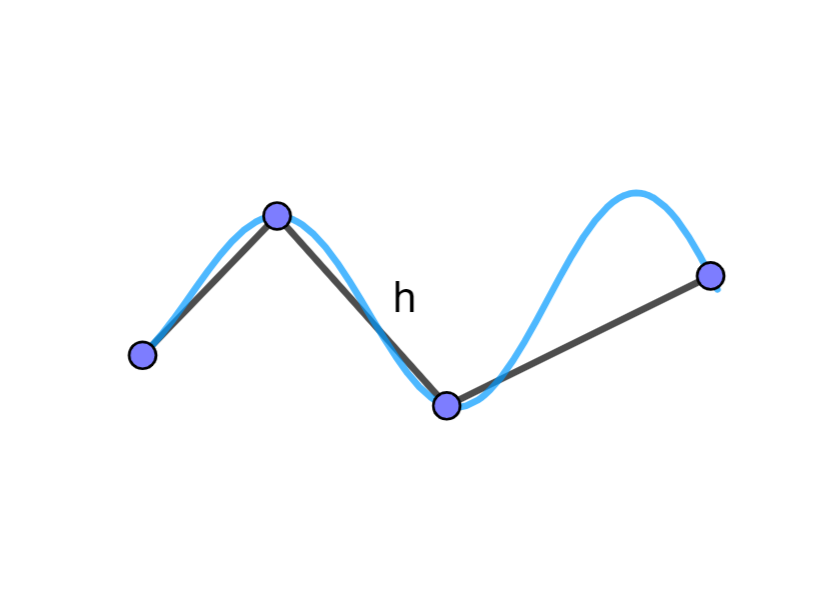
\includegraphics[width=0.33\textwidth]{Capitoli/Capitolo1/lunghezza1.png}
    \hspace{0.05\textwidth} % Spazio tra le immagini
    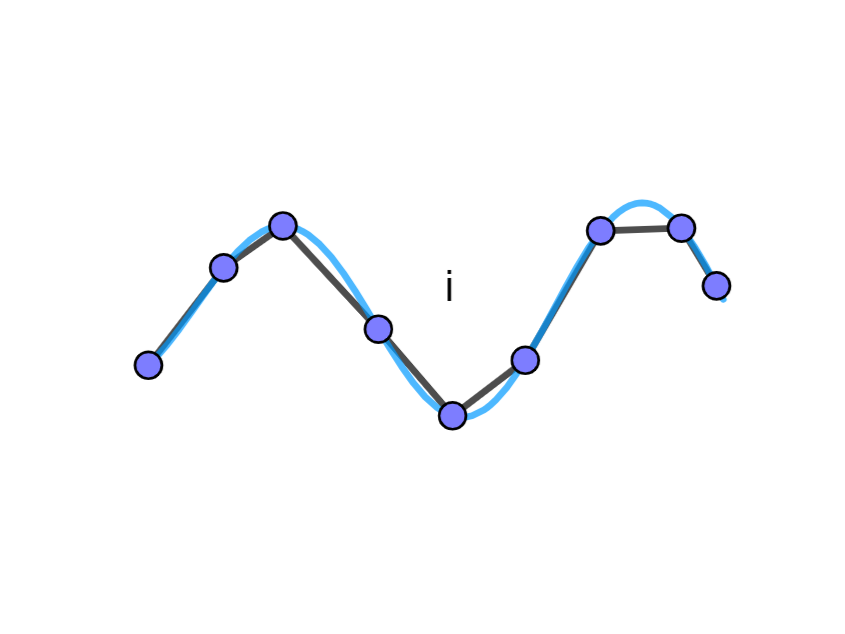
\includegraphics[width=0.33\textwidth]{Capitoli/Capitolo1/lunghezza2.png}
    \caption{In figura la stessa curva la cui lunghezza viene misurata con poligonali diverse.}
\end{figure}
\begin{definition}
    Sia $\varphi:[a,b]\to \mathbb{R}^n$, allora si dice \textbf{lunghezza di un arco di curva} continua la quantità
    \begin{equation}
        L(\varphi)=\sup\limits_{l}(\mathcal{P})
    \end{equation}
    dove $\mathcal{P} \in \Pi$ con $\Pi=\left\{\text{poligonali inscritte nella curva}\right\}$.
\end{definition}
\begin{definition}
    Si dice che una curva $\varphi: [a,b] \to \mathbb{R}^n$ è \textbf{rettificabile} se 
    \begin{equation}
        \sup\limits_{\mathcal{P}\in\Pi}L(\varphi)<+\infty
    \end{equation}
\end{definition}
\begin{theorem}[Teorema di rettificabilità]
Sia $\varphi: [a,b] \to \mathbb{R}^n$ una curva di classe $C^1$. Allora essa è rettificabile e 
\begin{equation}
    L(\varphi)=\int_{a}^{b}{|\varphi'(t)|dt}
\end{equation}
\end{theorem}
\begin{oss}
    La lunghezza di una curva $C^1$ è invariante per riparametrizzazione.
\end{oss}
\begin{oss}
    Si osservi che vale: $\ell(\mathcal{P})\leq \int_{a}^{b}{|\varphi'(t)|dt}$. Infatti:
    \begin{equation}
        \begin{aligned}
            \ell(\mathcal{P}) &= \sum\limits_{i=1}^{N} \left| \varphi(t_i) - \varphi(t_{i-1}) \right|= \sum\limits_{i=1}^{N} \left\lvert \int_{t_{i-1}}^{t_i} \varphi'(t) \, dt \right\rvert \\
            &\leq \sum\limits_{i=1}^{N} \int_{t_{i-1}}^{t_i} \left\lvert \varphi'(t) \right\rvert \, dt = \int_{a}^{b} \left\lvert \varphi'(t) \right\rvert \, dt
        \end{aligned}
    \end{equation}
\end{oss}
\begin{example}
    Detta 
    \begin{equation*}
        f(x)= \begin{cases}
            0 \text{ se } x=0\\ x\sin(\frac{1}{x}) \text{ se } x\neq 0
        \end{cases}
    \end{equation*}
    allora una curva non rettificabile può essere 
    \begin{equation*}
        \varphi(t)=(t, f(t)) \text{ con } t\in[0,1]
    \end{equation*}
\end{example}
\section{Triedro di Frénet}
Si desideri ora sviluppare un sistema di riferimento intrinseco ad una curva $\varphi:[a, b] \to \mathbb{R}^n$ regolare e tale che $\varphi'(t)$ ed il versore tangente $T$ siano ben definiti su $(a, b)$.
\begin{definition}
    Si definisce l'\textbf{ascissa curvilinea} o parametro d'arco $s=s(t)$ come
    \begin{equation}
        s(t)=\int_a^t{\left\lvert \varphi'(\tau) \right\rvert d\tau}
    \end{equation}
    \end{definition}
    \begin{oss}
        $s:[a,b] \to [0, L(\varphi)=L]$ è una parametrizzazione della curva regolare $\varphi$. Inoltre, $s'(t)=|\varphi'(t)| \neq 0$ su $(a,b)$.
    \end{oss} 
    \begin{oss}
        Riparametrizzando $\varphi$ con ascissa curvilinea $s=s(t)$, si può dire che $\varphi\sim\psi$. Dunque, rinominata $t(s)=s^{-1}(t)$, vale $\psi(s)=\varphi(t(s))$. Derivando la riparametrizzazione, si ha che:
        \begin{equation}
            \psi'(s)=\varphi'(t(s)) \text{ } t'(s) \overset{\substack{\text{Derivata}\\\text{ inversa}}}{=} \frac{\varphi'(t(s))}{s'(t)} = \frac{\varphi'(t(s))}{|\varphi'(t(s))|}
        \end{equation}
        Ciò mostra come il vettore tangente a $\psi$ sia in ogni punto un versore tangente $T(s)$
    \end{oss}

\paragraph*{Prodotto scalare in $\mathbb{R}^n$}
Siano $\underline{v}=(v_1, \dots, v_n)$ e $\underline{w}=(w_1, \dots, w_n)$ vettori di $\mathbb{R}^n$. Allora
\begin{equation}
    \langle \underline{v}, \underline{w} \rangle = \sum\limits_{i=1}^{n}{v_iw_i} 
\end{equation}
\paragraph*{Prodotto vettoriale in $\mathbb{R}^3$}
Siano $\underline{v}=(v_1, v_2, v_3)$ e $\underline{w}=(w_1, w_2, w_3)$ vettori di $\mathbb{R}^3$. Allora
\begin{equation}
    \underline{v} \wedge \underline{w}=
    \left\lvert\begin{matrix}
         e_1 & e_2 & e_3 \\
               v_1 & v_2 & v_3 \\
               w_1 & w_2 & w_3
            \end{matrix}\right\rvert
\end{equation}
\begin{lemma}
    Siano $u, v$ definiti in $I\to\mathbb{R}^3$ e derivabili. Allora:
    \begin{align}
        \frac{d}{dt}{\langle u(t), v(t) \rangle} = \langle u'(t), v(t) \rangle + \langle u(t), v'(t) \rangle \\
        \frac{d}{dt}\left(u(t) \wedge v(t)\right) = u'(t) \wedge v(t) + u(t) \wedge v'(t)
    \end{align}
\end{lemma}
\begin{proposition}
    Sia $w:I\to\mathbb{R}^3$ derivabile e tale che $\exists$ $c>0$ per cui $|w(t)|=c$ $\forall$ $t \in I$. Allora $w'(t) \perp w(t)$.
\end{proposition}
    \begin{proof}
        Affinché i due vettori siano ortogonali, occorre che il loro prodotto scalare sia nullo. Pertanto, poiché per ipotesi $|w(t)|=c$
        \begin{equation}
            |w(t)|^2=c^2 \iff \langle w(t), w(t) \rangle = c
        \end{equation}
        Derivando rispetto a $t$ e applicando l'equazione 1.26, si ha che:
        \begin{equation}
            \frac{d}{dt}{\langle w(t), w(t)\rangle}\overset{\substack{\text{Prop.} \\ \text{prod. scal.} }}{=}2 \langle w'(t), w(t) \rangle = \frac{d c^2}{dt}=0
        \end{equation}
    \end{proof}
\begin{oss}
    La curva $\psi:[c,d] \to \mathbb{R}^3$ parametrizzata con ascissa curvilinea è tale che $|\psi'(s)|=1$. Di conseguenza, per la proposizione, $\psi''(s) \perp \psi'(s)$ e, nella fattispecie, $T'(s) \perp T (s)$.  
\end{oss}
\begin{definition}
    Sia $\psi$ una riparametrizzazione di $\varphi$ biregolare nel suo intervallo di parametrizzazione, cioè sia tale che $\psi \in C^2([c,d])$ e $\psi''(s) \neq 0$ $\forall$ $s \in [c,d]$. Allora si può definire il \textbf{versore normale} il normalizzato della derivata del versore tangente. Quindi:
    \begin{equation}
        N(s)=\frac{\psi''(s)}{|\psi''(s)|}=\frac{T'(s)}{|T'(s)|}
    \end{equation}
\end{definition}
\begin{definition}
    Si dice \textbf{curvatura} di $\psi$ in $\psi(s)$ 
    \begin{equation}
        k(s)= |\psi''(s)|
    \end{equation}
\end{definition}
\begin{definition}
    Si dice \textbf{piano osculatore} per $\psi$ in $\psi(s)$ il piano generato da 
    \begin{equation}
        \left\{T(s), N(s)\right\}
    \end{equation} 
\end{definition}
È appena stato definito un nuovo versore $N$ linearmente indipendente. È possibile ottenere una base ortonormale di $\mathbb{R}^3$ attraverso il prodotto esterno dei due versori.
\begin{definition}
    Si dice \textbf{versore binormale} il versore:
    \begin{equation}
        B(s)=T(s) \wedge N(s)
    \end{equation}
\end{definition}
\begin{definition}
    Si dice \textbf{piano normale} per $\psi$ in $\psi(s)$ il piano generato da
    \begin{equation}
        \left\{N(s), B(s)\right\}
    \end{equation}
\end{definition}
\newpage
\begin{definition}
    Si dice \textbf{piano rettificato} per $\psi$ in $\psi(s)$ il piano generato da
    \begin{equation}
        \left\{ B(s), T(s) \right\}
    \end{equation}
\end{definition}
\begin{definition}
    Si dice \textbf{triedro di Frénet} o \textbf{terna intrinseca} la base ortonormale di $\mathbb{R}^3$ positivamente orientata formata da
    \begin{equation}
        \left\{T(s), N(s), B(s)\right\}
    \end{equation}
\end{definition}
\begin{theorem}[Formule di Frénet]
    Sia $\varphi: I \to \mathbb{R}^3$ una curva biregolare, di classe $C^3(I)$ e parametrizzata con ascissa curvilinea. Allora, $\exists!$ $k:I\to \mathbb{R}_+$, $\tau:I\to\mathbb{R}$ tali che:
    \begin{equation}
        \begin{cases}
            T'(s)=k(s)N(s)\\
            N'(s)=-k(s)T(s)-\tau(s)B(s)\\
            B'(s)=\tau(s)N(s)
        \end{cases}
    \end{equation}
    \end{theorem}
    \begin{proof}
        Si parta dalla prima equazione: 
        \begin{equation}
            T'(s)=k(s)N(s).        
        \end{equation}
        Tale risultato discende dalla definizione stessa di $T'$. Si consideri infatti che $T'(s)\perp T(s)$ poiché $|T(s)|=1$ $\forall$ $s$. Prendendo poi $k(s)=|T'(s)|$, si ottiene l'identità tra i due membri.\\
        Si analizzi poi la terza equazione:
        \begin{equation}
            B'(s)=\tau(s)N(s)
        \end{equation}
        Per definizione di $B$, esso discende dal prodotto vettoriale degli altri due versori. Se ne studi la derivata:
        \begin{equation}
            B'(s)=T'(s)\wedge N(s) + T(s) \wedge N(s) \overset{\substack{T'(s)\parallel N(s)}}{=} T(s)\wedge N'(s)
        \end{equation}
        Quindi, poiché $B'(s)\perp T(s)$ e $B'(s) \perp B(s)$, allora $B'(s) \parallel N(s)$. Definendo $\tau(s)=|B'(s)|$, l'equazione è soddisfatta.\\
        Infine, si affronti la seconda equazione:
        \begin{equation}
            N'(s)= -k(s)T(s)- \tau(s)B(s)
        \end{equation}
        Siccome $\left\{T(s), N(s), B(s)\right\}$ è positivamente orientata,
        \begin{equation}
            N(s)=B(s) \wedge T(s)
        \end{equation}
        Derivando $N$, si ha che
        \begin{equation}
            \begin{aligned}
                N'(s)&=B'(s)\wedge T(s) + B(s) \wedge T'(s)=\\
                &\overset{\substack{\text{Frénet}}}{=} \tau(s)N(s)\wedge T(s) + B(s) \wedge k(s)N(s)\\
                &\overset{\substack{N \wedge T = -B\\B \wedge N =-T}}{=} -\tau(s)B(s)- k(s)T(s)
            \end{aligned}
        \end{equation}
    \end{proof}
\begin{oss}
    Risolvendo il sistema di equazioni differenziali, si potrebbe mostrare come valga anche l'implicazione inversa.
\end{oss}
\begin{oss}
    Poiché $B(s)$ è ortogonale al piano osculatore, si può notare che se esso ha derivata nulla, il piano rimane costante.
\end{oss}
\begin{definition}
    Si dice \textbf{torsione} di $\varphi$ in $\varphi(s)$
    \begin{equation}
        \tau(s)=|B'(s)|
    \end{equation}
\end{definition}
\begin{definition}
    Una curva si dice \textbf{piana} se la sua torsione è nulla, cioè se essa giace su un piano.
\end{definition}
\begin{definition}
    Si dice \textbf{cerchio osculatore} per una curva $\varphi:[a,b]\to \mathbb{R}^3$ biregolare, il cerchio giacente nel piano osculatore, avente raggio $r=\frac{1}{k(t)}$ con $k(t)$ curvatura di $\varphi(t)$ e centro sul semiasse normale a $\varphi(t)$.
\end{definition}
\begin{definition}
    Il raggio del cerchio osculatore è detto \textbf{raggio osculatore}.
\end{definition}
Nel corso dell'ultimo capitolo si è cercato di trovare una parametrizzazione di una curva in $\mathbb{R}^3$ ed è stata proposta l'ascissa curvilinea, il cui calcolo non è però sempre comodo.\\
Pertanto è possibile osservare che se una generica $\psi:[a,b]\to \mathbb{R}^3$ è una curva riparametrizzata con parametro qualunque, allora valgono su di essa le formule di Frénet generalizzate.
\begin{theorem}[Formule di Frénet generalizzate]
    Sia $\psi$ una curva riparametrizzata con parametro qualunque su cui valgano le ipotesi del Teorema 2. Allora vale:
    \begin{equation}
        \begin{cases}
            T'(t)=|\psi'(t)| k(t) N(t)\\
            N'(t)=-|\psi'(t)| k(t) T(t) - |\psi'(t)| \tau(t)B(t)\\
            B'(t)=|\psi'(t)|\tau(t)N(t)
        \end{cases}
    \end{equation}
    Dove:
    \begin{align}
        &T(t)=\frac{\psi'(t)}{|\psi'(t)|} \label{Eq: Frenet Tangente}\\
        &N(t)=\frac{T'(t)}{|T'(t)|} \label{Eq: Frenet Normale}\\
        &B(t)=\frac{\psi'(t)\wedge \psi''(t)} {|\psi'(t)\wedge \psi''(t)|} \label{Eq: Frenet Binormale}\\
        &k(t)=\frac{|\psi'(t)\wedge\psi''(t)|}{|\psi'(t)|^3} \label{Eq: Frenet Curvatura}\\
        &\tau(t)=\frac{\langle\psi'(t)\wedge \psi''(t), \psi'''(t)\rangle}{|\psi'(t)\wedge \psi''(t)|^2} \label{Eq: Frenet Torsione}
    \end{align}    
\end{theorem}
\section{Integrale curvilineo}
\begin{definition}
    Sia $\gamma$ una curva regolare e $\varphi:[a,b]\to \mathbb{R}^n$ una sua rappresentazione parametrica. Sia poi $f:A\subseteq \mathbb{R}^n \to \mathbb{R}$ una funzione in più variabili tale che $\varphi([a,b])\subseteq A$ e $f \circ\varphi$ sia continua su $[a,b]$.\\
    Allora si può definire l'\textbf{integrale curvilineo di prima specie} di f su $\gamma$
    \begin{equation}
        \int_\gamma{fds} := \int_{a}^{b}{f(\varphi(t))|\varphi'(t)|dt}
    \end{equation}
\end{definition}
\begin{theorem}[Invarianza per equivalenza di curve]
    L'integrale curvilineo di prima specie è invariante per equivalenza di curve.
\end{theorem}
    \begin{proof}
        Si ricordino innanzitutto le ipotesi:\\
        \indent $\varphi:[a,b]\to \mathbb{R}^n$ regolare, parametrizzazione di $\gamma$.\\
        \indent $f:A\subseteq\mathbb{R}^n \to \mathbb{R}$ con $\varphi([a,b]) \subseteq A$\\
        \indent $\psi:[c, d]\to \mathbb{R}^n$ regolare, parametrizzazione di $\hat{\gamma}$ e $\varphi \sim \psi$.\\
        La tesi da mostrare è:
        \begin{equation}
            \int_\gamma{f ds}=\int_{\hat{\gamma}}{f ds}
        \end{equation}
        Per definizione dell'integrale curvilineo di prima specie si ha:
        \begin{equation}
            \int_\gamma{fds}= \int_{a}^{b}{f(\varphi(t))|\varphi'(t)|dt}
        \end{equation}
        Ponendo, $s=\eta(t)$ si ha che
        \begin{equation}
            \varphi(t)=\psi(\eta(t)) \iff \varphi(\eta^{-1}(s))=\psi(s)    
        \end{equation}
        e
        \begin{equation}
            \psi'(s)=\varphi'(\eta^{-1}(s))(\eta^{-1})'(s)
        \end{equation}
        Perciò, risolvendo l'integrale con la seguente sostituzione 
        \begin{equation}
            \begin{aligned}
            &s=\eta(t) \\ &t=\eta^{-1}(s) \\ &dt=(\eta^{-1})'(s)ds
            \end{aligned}
        \end{equation}
        si ha che
        \begin{equation}
            \begin{aligned}
                &\int_\gamma{fds} = \int_{a}^{b}{f(\varphi(t))\ |\varphi'(t)|\ dt}\\
                &\overset{\text{sub}}{=} \int_{\eta(a)}^{\eta(b)}{f(\varphi(\eta^{-1}(s)))\ |\varphi(\eta^{-1}(s))|\ (\eta^{-1})'(s)\ ds}
            \end{aligned}
        \end{equation}
        Ora, dipendentemente dalla monotonia di $\eta$ si avrà:\\
        \indent$\eta^{-1}>0 \Rightarrow \ \eta(a)=c,\  \eta(b)=d,\  (\eta^{-1})'(s)>0$
        \begin{equation}
            \begin{aligned}
                &\int_{\eta(a)}^{\eta(b)}{f(\varphi(\eta^{-1}(s)))\ |\varphi'(\eta^{-1}(s))| \ (\eta^{-1})'(s)\ ds}=\\
                &\int_{c}^{d}{f(\psi(s))\ |\psi'(s)| \ ds}= \int_{\hat{\gamma}}{f \ ds}
            \end{aligned}
        \end{equation}
        \indent$\eta^{-1}<0 \Rightarrow \eta(a)=d, \ \eta(b)=c, \ (\eta^{-1})'(s)<0$
        \begin{equation}
            \begin{aligned}
                &\int_{\eta(a)}^{\eta(b)}{f(\varphi(\eta^{-1}(s)))\ |\varphi'(\eta^{-1}(s))| \ (\eta^{-1})'(s)\ ds}=\\
                &\int_{d}^{c}{f(\psi(s))\ (-|\psi'(s)|)\ ds} = \int_{c}^{d}{f(\psi(s))\ |\psi'(s)|\ ds}= \int_{\hat{\gamma}}{f\ ds}
            \end{aligned}
        \end{equation}
    \end{proof}
    \begin{oss}
        La distinzione finale discende dal fatto che, presa l'equazione 1.55 e applicatovi il modulo, se $\eta$ è crescente, si ha
        \begin{equation}
            \begin{aligned}
                |\psi'(s)|&=|\varphi'(\eta^{-1}(s))(\eta^{-1})'(s)|\overset{\substack{\text{Prop.}\\\text{Norma}}}{=}|(\eta^{-1})(s)|\ |\varphi'(\eta^{-1}(s))=\\
                &\overset{\eta'>0}{=} (\eta^{-1})'(s)\ |\varphi'(\eta^{-1})(s)|
            \end{aligned}
        \end{equation}
        se $\eta$ è decrescente,
        \begin{equation}
            \begin{aligned}
                |\psi'(s)|&=|\varphi'(\eta^{-1}(s))(\eta^{-1})'(s)|\overset{\substack{\text{Prop.}\\\text{Norma}}}{=}|(\eta^{-1})(s)|\ |\varphi'(\eta^{-1}(s))=\\
                &\overset{\eta'<0}{=} -(\eta^{-1})'(s)\ |\varphi'(\eta^{-1})(s)|
            \end{aligned}
        \end{equation}
    \end{oss}
\begin{corollary}
    La lunghezza di una curva regolare a tratti è invariante per equivalenza.
    \end{corollary}
    \begin{proof}
        La dimostrazione del corollario discende dalla dimostrazione precedente, in cui $f \equiv 1$.
        Infatti si avrebbe:
        \begin{equation}
            L(\varphi)=\int_{a}^{b}{|\varphi'(t)|\ dt}=\int_{c}^{d}{|\psi'(s)|\ ds}=L(\psi)
        \end{equation}
    \end{proof}
    \begin{oss}
        Sia $\varphi$ una parametrizzazione della curva $\gamma$ mediante ascissa curvilinea. Allora,
        \begin{equation}
            \int_{\gamma}{f \ ds}= \int_{0}^{L}{f(\varphi(t))|\varphi'(t)|\ dt} \overset{\substack{|\varphi'(t)| \equiv 1\\ \text{per param.}}}{=} \int_{0}^{L}{f(\varphi(t))\ dt}
        \end{equation}
        è proprio l'area sottesa da $f\Big|_{\gamma}$
    \end{oss}\cleardoublepage
\chapter{Funzioni in più variabili}
All'interno di questo capitolo si affronterà lo studio sistematico delle proprietà di funzioni in più variabili reali.\\
Nello specifico, si considereranno funzioni della forma: 
\begin{equation}
    f:\mathbb{R}^n \to \mathbb{R}^m
\end{equation}
con $m=1$, le cosiddette funzioni scalari, per poi passare al caso $m>1$, cioè le funzioni a valori vettoriali.
\section{Richiami di topologia in $\mathbb{R}^n$}
Per poter trattare lo studio di funzioni in più variabili occorre prima studiare la topologia dello spazio in cui si lavora.
In particolare, si può osservare che $\mathbb{R}^n$ è uno spazio vettoriale euclideo \textbf{normato}.
\begin{definition}
    Si dice che uno spazio $\mathbb{K}^n$ è \textbf{normato} se per ogni suo elemento $x=(x_1,\dots,x_n) \in \mathbb{K}^n$ la norma è ben definita. Nel caso di $\mathbb{R}^n$, si ha che:
    \begin{equation}
        |x|=\sqrt{\sum\limits_{i=1}^{n}{x_i^2}}
    \end{equation}
\end{definition}
Tramite la definizione di norma si può ottenere la definizione di \textbf{distanza}, grazie alla quale $\mathbb{R}^n$ può essere definito anche come spazio metrico.
\begin{definition}
    Sia $X$ un insieme e sia $d:X \times X \to \left[0, +\infty \right)$ una funzione che ad ogni coppia $(x,y)$ di punti di $X$ associa un numero reale $d(x,y)\geq0$. Allora si dice che $d$ è una \textbf{distanza} su $X$ se sono verificate le seguenti condizioni:
    \begin{align}
        &d(x,y)=0 \ \iff x=y \qquad\forall\ x,y \in X \\
        &d(x,y)=d(y,x) \qquad \forall\ x,y \in X \\
        &d(x,y) \leq d(x,z) + d(z, y) \qquad \forall\ x,y,z \in X
    \end{align}
    In particolare in $\mathbb{R}^n$ si ha che:
    \begin{equation}
        d(x, y)=|x-y|
    \end{equation}
\end{definition}
\begin{definition}
    Sia $x_0$ un elemento di $\mathbb{R}^n$ fissato e sia $\delta>0$ un intero fissato. Si dice \textbf{intorno sferico} di $x_0$ di raggio $\delta$ la sfera aperta e non vuota di centro $x_0$ definita analiticamente come:
    \begin{equation}
        B_\delta(x_0)=\left\{x \in \mathbb{R}^n \ \mid \ d(x, x_0) < \delta \right\}
    \end{equation}
    \end{definition}
    \begin{oss}
        Si noti che con \textit{aperta} si intende dire che nell'intorno sferico non sono presenti elementi tali che $d(x, y)=\delta$.
    \end{oss}
    \begin{example}
        Un esempio di intorno sferico può essere la circonferenza in $\mathbb{R}^2$ di raggio $\delta=1$ centrata in $(x_0, y_0) \in \mathbb{R}^2$ definita come:
        \begin{equation*}
            B_1(x_0, y_0)= \{(x,y) \in \mathbb{R}^2 \ \mid \ \sqrt{(x-x_0)^2+(y-y_0)^2}< 1\}
        \end{equation*}
    \end{example}
\begin{definition}
    Siano $E \subseteq \mathbb{R}^n$ e $x_0 \in \mathbb{R}^n$. Allora $x_0$ è detto \textbf{punto interno} per $E$ se 
    \begin{equation}
        \exists\ \delta>0 \text{ tale che } B_\delta(x_0) \subseteq E 
    \end{equation}
    Si indica poi l'insieme dei punti interni di $E$ con $\mathring{E}$ oppure con int(E).
\end{definition}
\begin{definition}
    Siano $E \subseteq \mathbb{R}^n$ e $x_0 \in \mathbb{R}^n$. Allora $x_0$ è detto \textbf{punto esterno} per $E$ se 
    \begin{equation}
        \exists \ \delta>0 \text{ tale che } B_\delta(x_0) \subseteq E^\complement = \mathbb{R}^n \setminus E
    \end{equation}
    Si indica poi l'insieme dei punti esterni di $E$ con ext(E).
\end{definition}
\begin{definition}
    Siano $E \subseteq \mathbb{R}^n$ e $x_0 \in \mathbb{R}^n$. Allora $x_0$ è detto \textbf{punto di frontiera} per $E$ se 
    \begin{equation}
        \forall \ \delta>0 \text{ si ha che } B_\delta(x_0) \cap E \neq \emptyset \land B_\delta(x_0) \cap E^\complement \neq \emptyset 
    \end{equation}
    Si indica poi l'insieme dei punti di frontiera di $E$ con $\partial{E}$.
\end{definition}
\begin{definition}
    Siano $E \subseteq \mathbb{R}^n$ e $x_0 \in \mathbb{R}^n$. Allora $x_0$ è detto \textbf{punto di accumulazione} per $E$ se 
    \begin{equation}
        \forall \ \delta>0 \text{ si ha che } B_\delta(x_0) \cap \left(E \setminus \{x_0\}\right) \neq \emptyset
    \end{equation}
\end{definition}
\begin{definition}
    Siano $E \subseteq \mathbb{R}^n$ e $x_0 \in \mathbb{R}^n$. Allora $x_0$ è detto \textbf{punto isolato} se esso appartiene alla frontiera di $E$ ma non è di accumulazione.
\end{definition}
\begin{proposition}
    L'insieme dei punti interni, esterni e di frontiera di $E \in \mathbb{R}^n$ è una partizione di $\mathbb{R}^n$.
\end{proposition}
\begin{example}
    Sia $E$ così definito:
    \begin{equation*}
        E \subseteq \mathbb{R}^2 \mid E= B_1(0,0) \cup \{(x,y) \in \mathbb{R}^2\ \mid \ x>0, \ x^2+ y^2=1\} \cup \left\{\left(1,\tfrac{3}{2}\right)\right\}
    \end{equation*}
    \begin{minipage}{0.3\textwidth}
        \centering
        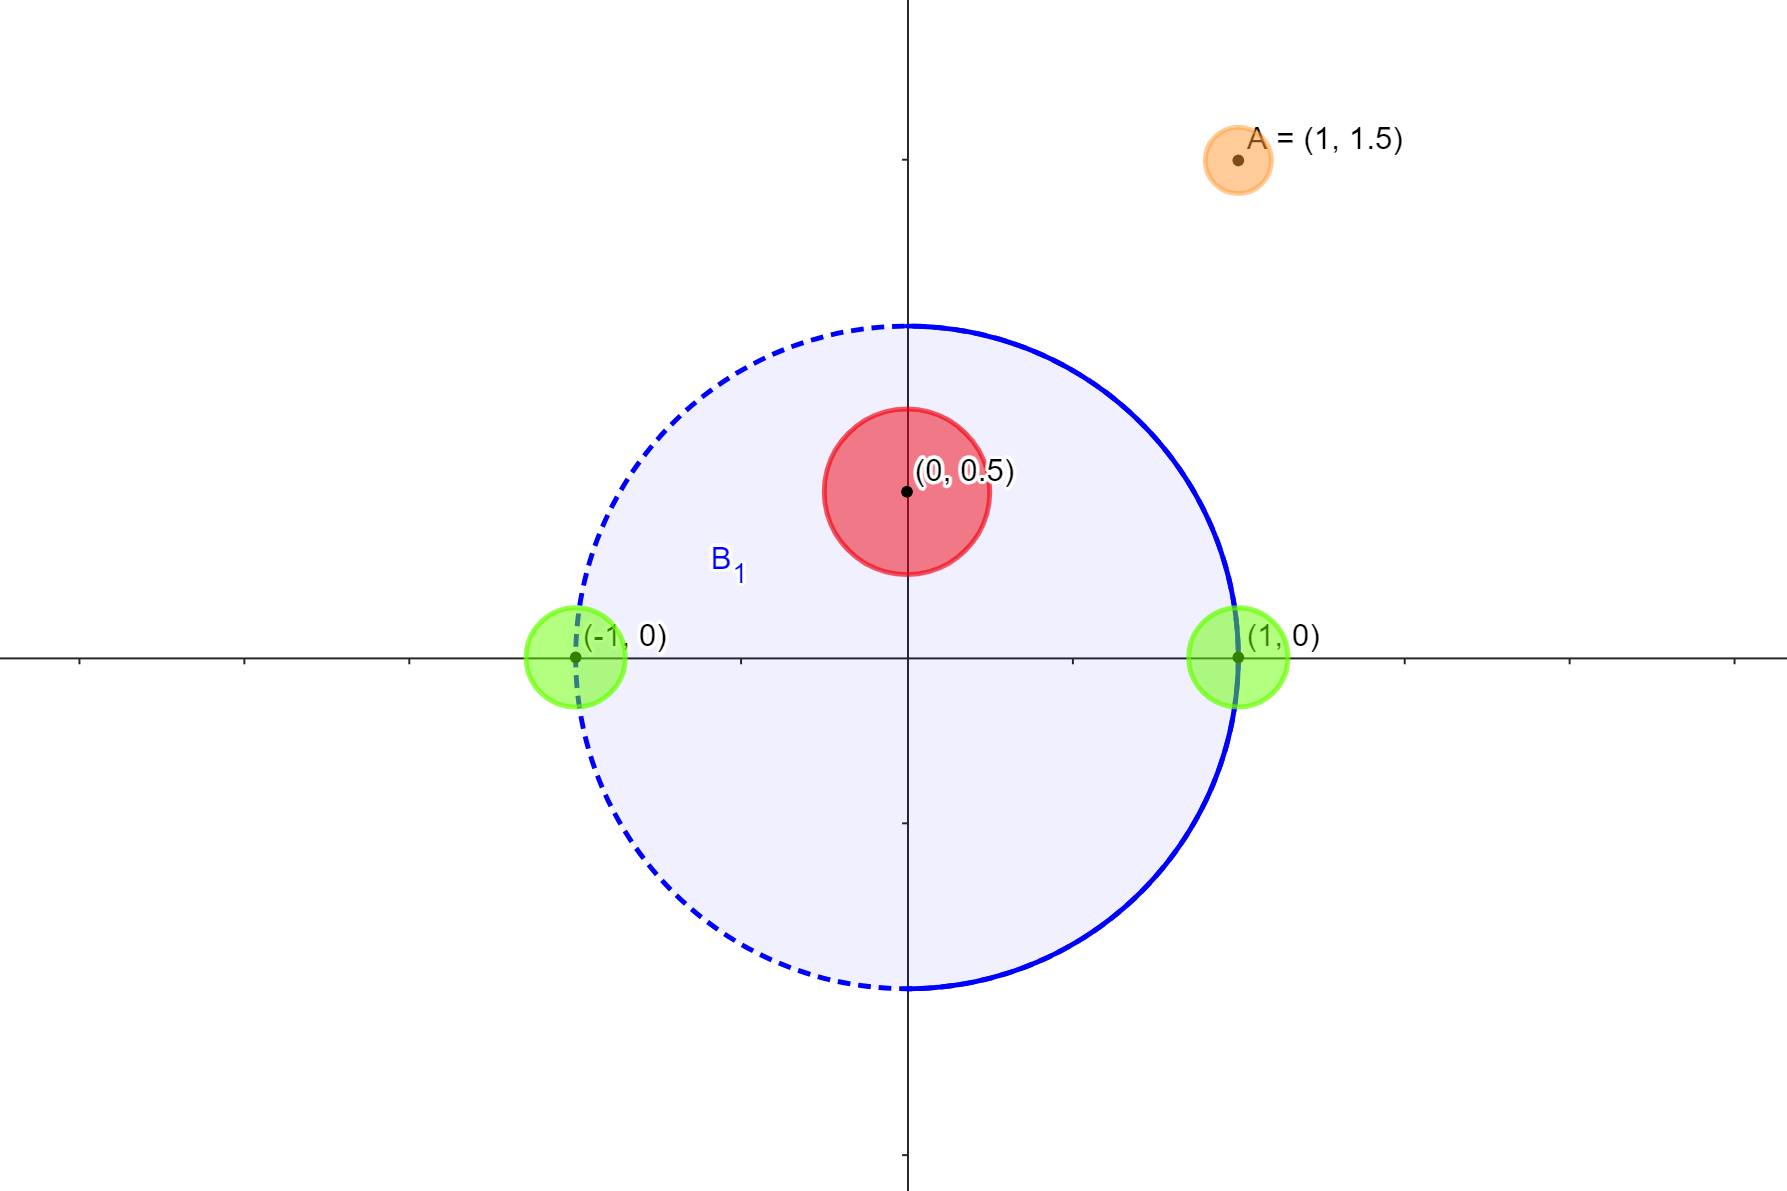
\includegraphics[width=\textwidth]{Capitoli/Capitolo2/Punti2.png}
    \end{minipage}
    \hfill
    \begin{minipage}{0.55\textwidth} 
        Si può dunque osservare che:
        \begin{itemize}
            \item $(0, \tfrac{1}{2})$ è \textit{interno}.
            \item $(1,0) $ è di \textit{frontiera} e di \textit{accumulazione}.
            \item $(-1,0) $ è di \textit{frontiera} e di \textit{accumulazione}.
            \item $\left(1, \tfrac{3}{2}\right) $ è di \textit{frontiera} e \textit{isolato}.
        \end{itemize}      
    \end{minipage}
\end{example}
\begin{definition}
    Un insieme $E \subseteq \mathbb{R}^n$ si dice \textbf{aperto} se
    \begin{equation}
        E=\mathring{E} \text{ oppure } E \cap \partial{E} = \emptyset
    \end{equation}
    ovvero se non ha punti esterni.
\end{definition}
\begin{definition} \label{Def: Insieme chiuso e chiusura}
    Si dice che un insieme $E \subseteq \mathbb{R}^n$ è \textbf{chiuso} se 
    \begin{equation}
        \partial{E} \subseteq E
    \end{equation}
    ovvero se $E^\complement$ è aperto.\\
    Si definisce poi \textbf{chiusura} di $E$ l'insieme
    \begin{equation}
        \overline{E} = E \cap \partial{E}
    \end{equation}
    Quindi un'altra definizione di insieme chiuso è:
    \begin{equation}
        E \text{ chiuso } \iff E=\overline{E}
    \end{equation}
\end{definition}
\begin{proposition}
    Un insieme $E$ è chiuso $\iff$ $E$ contiene tutti i suoi punti di accumulazione.
\end{proposition}
\begin{oss}
    $E=\{x_0\}$ con $x_0 \in \mathbb{R}^n$ fissato è chiuso e $E=\partial{E}$.
\end{oss}
\begin{oss}
    Dalla definizione, $\emptyset$ e $\mathbb{R}^n$ sono entrambi contemporaneamente aperti e chiusi e sono gli unici sottoinsiemi di $\mathbb{R}^n$ con tali proprietà.
\end{oss}
\begin{definition}
    Sia $E \subseteq \mathbb{R}^n$, $E$ si dice \textbf{limitato} se
    \begin{equation}
        \exists R>0 \text{ tale che } E \subseteq B_R(0)
    \end{equation}
    Altrimenti esso è detto \textbf{illimitato}.
\end{definition}
\begin{definition}
    Un insieme aperto $A\subseteq \mathbb{R}^n$ si dice \textbf{connesso} se non esistono due aperti $A_1, \ A_2$ non triviali (cioè diversi da $\emptyset,\ \mathbb{R}^n,\ A$) e disgiunti tali che
    \begin{equation}
        A=A_1 \cup A_2
    \end{equation}
\end{definition}
\begin{definition}
    Sia $E \subseteq \mathbb{R}^n$. Allora $E$ si dice \textbf{connesso per archi} se per ogni $(x,y) \in E$ esiste una curva parametrica $\varphi:[0,1] \to E$ tale che
    \begin{equation}
        \varphi(0)=x \land \varphi(1)=y
    \end{equation}
\end{definition}
\begin{definition}
   $E \subseteq \mathbb{R}^n$ si dice \textbf{dominio} (\textbf{connesso}) se è la chiusura di un aperto (connesso).
\end{definition}
\begin{definition}
    Un insieme $E \subseteq \mathbb{R}^n$ si dice \textbf{convesso} se, definito $[x,y]$ il segmento di estremi $x,\ y$ si ha che
    \begin{equation}
        [x,y] \subseteq E
    \end{equation}
    \end{definition}
    \begin{oss}
        Un insieme convesso è per definizione connesso per archi.
    \end{oss}
\begin{definition}
    Un insieme $E \subseteq \mathbb{R}^n$ si dice \textbf{stellato} rispetto ad un punto $x_0$ di E se per ogni $x$ di $E$ si ha che
    \begin{equation}
        [x_0, x] \subseteq E
    \end{equation}
\end{definition}

%%  DEFINIZIONI SEQUENZIALI


\section{Definizioni sequenziali}
\begin{definition}
    Si dice \textbf{successione in $\mathbb{R}^n$} una funzione da $\mathbb{N}$ a valori in $\mathbb{R}^n$.
    \begin{equation}
        (x_k)_{k \in \mathbb{N}} = ((x_k)_1, \dots, (x_k)_n)  
    \end{equation}
    con $k \in \mathbb{N}$ indice intero della successione.
\end{definition}
\begin{definition}
    Sia $(x_k)_k$ una successione in $\mathbb{R}^n$. Si dice che $x_k$ \textbf{converge} a $\ell$, cioè
    \begin{equation}
        x_k \to \ell=(\ell_1, \dots, \ell_n) \in \mathbb{R}^n
    \end{equation}
    se la loro distanza converge a zero. Poiché 
    \begin{equation}
        d(x_k, \ell)=|x_k-\ell|=\sqrt{[(x_k)_1-\ell_1]^2+\dots+[(x_k)_n-\ell_n]^2}
    \end{equation}
    la successione converge se ogni sua componente converge a ciascuna componente di $\ell$, quindi
    \begin{equation}
        (x_k)_k \overset{k\to+\infty}{\to} \ell \iff (x_k)_i \overset{k\to+\infty}{\to} \ell_i \ \forall i
    \end{equation}
\end{definition}
\begin{definition}
    Sia $(x_k)_k$ una successione di vettori di $\mathbb{R}^n$. Si dice che $x_k$ \textbf{diverge} se
    \begin{equation}
        |x_k| \overset{k\to+\infty}{\to} \infty
    \end{equation}
    \end{definition}
    \begin{oss}
        Si osservi che è sufficiente che la norma di una sola componente di $x_k$ diverga affinché la successione sia divergente.
        \begin{example}
            Presa come successione $x_k=\left(\frac{1}{k}, k\right)$, poiché la sua seconda componente è divergente per $k \to \infty$, anche la successione lo è.
        \end{example}
    \end{oss}
\begin{definition} \label{Def: Punto di accumulazione}
    Sia $E \subseteq \mathbb{R}^n$ e sia $x_0 \in \mathbb{R}^n$. Si dice che $x_0$ è \textbf{punto di accumulazione} per $E$ se
    \begin{equation}
        \exists\ (x_k)_k \text{ con } x_k\neq x_0 \in E \ \forall \ k \text{ tale che } x_k \to x_0
    \end{equation}
\end{definition}
\begin{definition}
    Sia $K \subseteq \mathbb{R}^n$. Si dice che $K$ è un insieme \textbf{compatto} se da ogni successione $(x_k)_k$ è possibile estrarre una sottosuccessione convergente ad un punto di $K$
\end{definition}
\begin{theorem}[Heine-Borel] \label{Teo: Heine Borel}
    Un insieme $K$ è compatto se e solo se è chiuso e limitato.
\end{theorem}
    \begin{oss}
        Un insieme $C \subseteq \mathbb{R}^n$ è chiuso se e solo se per ogni successione di elementi in $C$ convergente si ha che il limite di tale successione è contenuto in $C$.
    \end{oss}

%%  INTRODUZIONE FUNZIONI IN PIU VARIABILI

\section{Introduzione alle funzioni in più variabili}
Come già anticipato, da questo momento in avanti si studieranno prima le funzioni scalari e poi quelle a valori vettoriali.
Si cominci prima da alcune definizioni di carattere generale. 
\begin{definition}
    Si dice \textbf{dominio} di una funzione $f$ di $n$ variabili il più grande sottoinsieme di $\mathbb{R}^n$ su cui $f$ è definita. Esso viene indicato con $\text{dom}(f)$.
\end{definition}
\begin{definition}
    Sia $f: \Omega \subseteq \mathbb{R}^n \to \mathbb{R}$. Si dice \textbf{grafico} di $f$ il sottoinsieme di $\mathbb{R}^{n+1}$
    \begin{equation}
        G(f)= \left\{(x_1, \dots, x_n, x_{n+1}) \in \Omega \times \mathbb{R} \mid x_{n+1}=f(x)\right\}
    \end{equation}
\end{definition}
\begin{definition}
    Sia $f:\Omega \subseteq \mathbb{R}^n \to \mathbb{R}$ e sia $l \in \mathbb{R}$. Si dice \textbf{superficie di livello} o \textbf{ipersuperficie} $l$ per $f$ il sottoinsieme
    \begin{equation}
        L_l=\left\{x \in \Omega \mid f(x)=l\right\}=f^{-1}(l)
    \end{equation}
\end{definition}

%%   LIMITI
\section{Limiti}
\begin{definition}[Limiti al finito] \label{Def: Limiti al finito}
    Sia $f:\Omega \subseteq \mathbb{R}^n \to \mathbb{R}$ e sia $x_0$ un punto di accumulazione per l'insieme $\Omega$.\\
    Si dice che $f$ \textbf{converge} a $\ell \in \mathbb{R}$ per $x \to x_0$ e si scrive
    \begin{equation}
        \lim_{x \to x_0}{f(x)}=\ell
    \end{equation} 
    se
    \begin{equation}
        \forall \varepsilon>0 \ \exists\delta=\delta_\varepsilon>0\ \text{tale che, se}\ 
                x \in B_\delta(x_0) \setminus \left\{x_0\right\}\ \cap\ \Omega
            \text{ allora}\ |f(x)-\ell|<\varepsilon
    \end{equation}
    Analogamente, si dice che $f$ \textbf{diverge} per $x \to x_0$ con $x \in \Omega$ e si scrive
    \begin{equation}
        \lim_{x \to x_0}{f(x)}=\underset{-\infty}{+\infty}
    \end{equation}
    se 
    \begin{equation}
        \forall M>0 \ \exists\delta=\delta_M>0\ \text{tale che, se}\ 
        x \in B_\delta(x_0) \setminus \left\{x_0\right\}\ \cap\ \Omega
            \text{ allora}\ \underset{f(x)<-M}{f(x)>M}
    \end{equation}
\end{definition}
\begin{definition}
    Sia $f:\Omega \subseteq \mathbb{R}^n$ con $x_0$ punto di accumulazione. Si dice che 
    \begin{equation}
        \lim_{x \to x_0}{f(x)}=\ell
    \end{equation}
    se per ogni successione di punti di $\Omega$ $(x_k)_k$ diversi da $x_0$ tali che
    \begin{equation}
        f(x_k)\to \ell
    \end{equation}
    \end{definition}
    \begin{oss}
        La definizione è analoga per i casi in cui $\ell$ sia infinito.
    \end{oss}
    \begin{oss}
        Stando alla definizione \ref{Def: Punto di accumulazione}, l'ipotesi di di $x_0$ punto di accumulazione garantisce l'esistenza di almeno una successione convergente.
    \end{oss}
\begin{definition}[Limiti all'infinito] \label{Def: Limiti all'infinito}
    Sia $f:\Omega \to \mathbb{R}$. Allora, 
    \begin{equation}
        \lim_{x \to \infty}{f(x)}=\ell
    \end{equation}
    se
    \begin{equation}
        \forall \varepsilon > 0 \ \exists k=k_\varepsilon>0 \ \text{tale che, se}\ |x|>k_\varepsilon,\ \text{allora}\ |f(x)-\ell|<\varepsilon
    \end{equation}
    Analogamente,
    \begin{equation}
        \lim_{x \to \infty}{f(x)}=\underset{-\infty}{+\infty}
    \end{equation}
    se 
    \begin{equation}
        \forall M>0 \exists k=k_M>0 \ \text{tale che, se}\ |x|>k_M\ \text{allora}\ \underset{f(x)<-M}{f(x)>M}
    \end{equation}
\end{definition}
\subsection{Metodi per la risoluzione di limiti}
Il discorso che segue parte dal caso specifico di funzioni in due variabili ma può essere generalizzato con le dovute accortezze al caso di funzioni in $n$ variabili.\\
Si parta dallo specificare che anche per i limiti di funzioni multivariabile è possibile utilizzare le approssimazioni asintotiche.\\
Stando alla definizione di limite, esso non deve dipendere da come ci si avvicina a $x_0$. In prima istanza occorre allora scegliere uno degli innumerevoli metodi per farlo, noti come restrizioni. Tramite questi, è possibile trovare un candidato limite la cui esistenza deve essere verificata in uno dei modi che verranno illustrati.\\
Si può osservare che, se la funzione tende ad un limite $\ell$, allora esso è unico e valgono i teoremi delle funzioni in una variabile su somme, prodotti e quozienti di limiti; inoltre, se il limite esiste, $f$ tende (e deve tendere) a $\ell$ lungo ogni sua possibile restrizione. Viceversa, se esistono almeno due restrizioni il cui limite sia differente, il limite non esiste.\\
L'approccio per trovare il candidato limite ammette
\begin{itemize}
    \item Restrizioni lungo grafici di funzioni di $x$ o $y$ passanti per $(x_0, y_0)$ e appartenenti al dominio di $f$. In tal caso le funzioni possono essere $y= \varphi(x)$ o $x=\psi(y)$ e si avrà
    \begin{equation}
    \lim_{x \to x_0} f(x, \varphi(x)) \text{ o } \lim_{y \to y_0}{f(\psi(y), y)}
    \end{equation}
    \item Restrizioni lungo successioni $(x_n, y_n) \to (x_0, y_0)$ e in tal caso si calcola
    \begin{equation}
        \lim_{n \to +\infty}{f(x_n,y_n)}
    \end{equation}
    \item Restrizioni lungo curve parametriche $(x(t), y(t)): I \to \mathbb{R}^2$ passanti per $(x_0, y_0)$. In tal caso si calcola
    \begin{equation}
        \lim_{t \to t_0}{f(x(t), y(t))}
    \end{equation}
\end{itemize}
Si mostrino di seguito alcuni modi per provare l'esistenza del limite.
\paragraph{Definizione}
Per conseguire il risultato prefissato occorre maggiorare o minorare la funzione in maniera tale da trovare un $\delta_\varepsilon$ per cui la definizione di limite sia verificata.
\begin{example}
    Si mostri il procedimento sul seguente limite.
    \begin{equation*}
        \lim_{(x,y) \to (0,0)}x
    \end{equation*}
    Attraverso la restrizione $(0,y)$ si può osservare che il candidato limite è $0$. Ora occorre provare che ciò sia vero.
    Dunque bisogna capire se sia possibile trovare un $\delta$ dipendente da $\varepsilon$ per cui sotto l'ipotesi
    \begin{equation*}
        \begin{cases}
            0<|(x,y)-(0,0)|<\delta\\
            (x,y) \in \text{dom}f
        \end{cases}
    \end{equation*}
    si abbia $|x-0|<\varepsilon$.\\
    Fissato $\varepsilon$ e sapendo che $|x|=\sqrt{x^2+y^2}<\delta$, serve provare che $|x|<\varepsilon$. Ciò è vero scegliendo $\delta<\varepsilon$.\\
    Al contrario, preso qualsiasi altro valore di $\ell$ la definizione non è verificata, come ci si aspetta.
\end{example}
\paragraph{Confronto}
Così come avveniva nelle funzioni a una variabile, è possibile verificare un candidato limite maggiorandolo e minorandolo con funzioni convergenti al medesimo candidato limite, applicando, cioè, il metodo del confronto.
\begin{example}
    Si calcoli il limite seguente.
    \begin{equation*}
        \lim_{(x,y) \to (0,0)}{\frac{xy}{\sqrt{x^2+y^2}}}
    \end{equation*}
    Tramite la restrizione su uno dei due assi si ottiene $0$ come candidato limite.
    Siccome vale la disuguaglianza di Young, che afferma che 
    \begin{equation*}
        xy \leq \frac{x^2+y^2}{2}
    \end{equation*}
    si può verificare che
    \begin{equation*}
        0 \leq \left|\frac{xy}{\sqrt{x^2+y^2}}\right| \leq \frac{\sqrt{x^2+y^2}}{2}
    \end{equation*}
    con gli estremi convergenti a $0$. Pertanto, il limite esiste ed è $0$.
\end{example}
\paragraph{Coordinate polari}
Dal momento che per provare la definizione di limite si deve controllare una distanza, può essere utile passare alle coordinate polari centrate nel punto $(x_0, y_0)$, ottenendo
\begin{equation}
    \begin{cases}
        x=x_0+ \varrho \cos(\theta)\\
        y=y_0+ \varrho \sin(\theta)
    \end{cases}
\end{equation}
Così facendo, fissato $\theta$ e fatto convergere $\varrho \to 0^+$, il limite diventa
\begin{equation}
    \lim_{\varrho\to 0}{f(x_0+\varrho\cos(\theta), y_0+\varrho\sin(\theta))}=\ell
\end{equation}
Si consegue così una condizione necessaria per l'esistenza del limite. È tuttavia possibile estendere tale affermazione ad una condizione necessaria e sufficiente ricercando un criterio tale da rendere il risultato univocamente determinato da $\varrho$ (e valido così $\forall\ \theta$).
\begin{theorem} \label{Teo: Condizione necessaria e sufficiente per un limite}
    Sia $f(x,y): E \subseteq \mathbb{R}^2 \to \mathbb{R}$ e sia $(x_0, y_0)$ punto di accumulazione per $\text{dom}f$ e sia $\ell \in \mathbb{R}$. Allora esiste
    \begin{equation}
        \lim_{(x,y)\to(x_0, y_0)}f(x,y)=\ell
    \end{equation}
    se e solo se esistono $r>0$ e $g:(0, r) \to \mathbb{R}$ tali che
    \begin{equation}
        \lim_{\varrho \to 0^+}{g(\varrho)=0}
    \end{equation}
    e, per ogni $\theta \in [0, 2\pi],\ \varrho\in (0, r)$ si ha che 
    \begin{equation}
        \left|f(x_0+\varrho\cos(\theta), y_0+\varrho\sin(\theta))-\ell \right|\leq g(\varrho)
    \end{equation}
\end{theorem}
\begin{example}
    Si calcoli nuovamente questo limite.
    \begin{equation*}
        \lim_{(x, y) \to (0,0)}{\frac{xy}{\sqrt{x^2+y^2}}}
    \end{equation*}
    Come prima, il candidato limite è $0$.\\
    Applicando un cambio di coordinate si ha che
    \begin{equation*}
        \begin{cases}
            x=\varrho\cos(\theta)\\
            y=\varrho\sin(\theta)
        \end{cases}
    \end{equation*}
    e, dunque, $f$ diviene
    \begin{equation*}
        f(\varrho\cos(\theta),\varrho\sin(\theta))=\frac{\varrho^2\cos(\theta)\sin(\theta)}{\varrho}=\varrho\cos(\theta)\sin(\theta)
    \end{equation*}
    Di conseguenza,
    \begin{equation*}
        |f(\varrho\cos(\theta),\varrho\sin(\theta))- \ell|=\varrho\cos(\theta)\sin(\theta) \leq \varrho = g(\varrho)
    \end{equation*}
    Pertanto, il limite esiste ed è verificato.
\end{example}
\begin{example}
    Si fornisca ora un esempio di limite non definito.
    \begin{equation*}
        \lim_{(x,y) \to (0,0)}{\frac{xy}{x^2+y^2}}
    \end{equation*}
    Per dimostrare l'inesistenza di $\ell$ si può procedere innanzitutto sfruttando le restrizioni. Infatti, se prendendo come cammini gli assi, il candidato limite è $0$, prendendo una retta generica della forma $y=mx$ tale risultato non è comprovato.
    \begin{equation*}
        \lim_{(x, mx) \to (0,0)}{\frac{x^2m}{x^2+x^2m^2}}=\lim_{(x, mx) \to (0,0)}{\frac{m}{m^2+1}} \neq 0
    \end{equation*}
    In alternativa, si può verificare ciò con il teorema \ref{Teo: Condizione necessaria e sufficiente per un limite}. In coordinate polari il limite diviene
    \begin{equation*}
        \lim_{\varrho \to 0^+}{\left|\frac{\varrho^2\cos(\theta)\sin(\theta)}{\varrho^2}\right|}=\lim_{\varrho \to 0^+}{\left|\cos(\theta)\sin(\theta)\right|} < \frac{1}{2}=g(\varrho)
    \end{equation*}
    Ma $g(\varrho)$ non tende a $0$ per $\varrho \to 0^+$ quindi, il limite si riconferma indefinito.
\end{example}
\subsection{Continuità}
Si sfruttino ora le nozioni apprese sui limiti per definire la continuità di una funzione.
\begin{definition} \label{Def: Continuità}
    Sia $f: E \subseteq \mathbb{R}^n \to \mathbb{R}$ e sia $x_0 \in \mathbb{R}^n$. Se $x_0$ è un punto isolato di E, la funzione si dice \textbf{continua} in $x_0$ per convenzione. Se $x_0$ è di accumulazione per E, f è \textbf{continua} in $x_0$ se è definita in tale punto e
    \begin{equation} \label{Eq: Continuità}
        \lim_{x \to x_0} f(x)= f(x_0)
    \end{equation}
    ovvero, in termini di $\varepsilon$ e $\delta$, se
    \begin{equation}
        \forall \varepsilon > 0 \  \exists \delta>0 \text{ tale che se } x \in B_\delta(x_0) \cap E, \ |f(x)-f(x_0)|< \varepsilon
    \end{equation}
    \end{definition}
    \begin{oss}
        Se f non è definita in $x_0$ ma esiste il limite $\ell$ di $f(x)$ per $x \to x_0$, è possibile definire il \textbf{prolungamento di continuità} per $f$ in $x_0$ come:
        \begin{equation}
            g(x) = \begin{cases}
                f(x) \text{ se } x \neq x_0, x \in \text{dom}f\\
                \ell \text { se } x=x_0
            \end{cases}
        \end{equation}
    \end{oss}
    \begin{oss}
        Rientrano tra le funzioni continue somme, prodotti, quozienti (ben definiti) di polinomi
    \end{oss}
\vspace*{\baselineskip}
Si noti che anche per funzioni in più variabili continue vale un analogo del teorema di \textbf{permanenza del segno}, che afferma che, se $f$ è definita in $B_\delta(x_0)$ ed è continua in $x_0$ con $f(x_0) \gtrless 0$, allora esiste $B_\delta'(x_0)$ con $\delta' \leq \delta$ su cui il segno viene mantenuto.
\begin{definition}
Sia $f:X \subseteq \mathbb{R}^n \to \mathbb{R}$. Si dice che $x_0 \in X$ è \textbf{punto di massimo assoluto} (forte) per $f$ in $X$ se
\begin{equation}
    \begin{aligned}
        f(x) \leq f(x_0) \ \forall x  \in X \\
        (f(x) < f(x_0) \ \forall x  \in X)
    \end{aligned}
\end{equation}
In tal caso, $f(x_0)$ è detto \textbf{valore massimo} di $f$ su $X$.\\
In maniera del tutto analoga, data $f:X \subseteq \mathbb{R}^n \to \mathbb{R}$, si dice che $x_0 \in X$ è \textbf{punto di minimo assoluto} (forte) per $f$ in $X$ se
\begin{equation}
    \begin{aligned}
        f(x) \geq f(x_0) \ \forall x \in X\\
        (f(x)>f(x_0) \ \forall x \in X)
    \end{aligned}
\end{equation}
In tal caso, $f(x_0)$ è detto \textbf{valore minimo} di $f$ su $X$
\end{definition}
\begin{theorem}[Weierstrass] \label{Teo: Weierstrass}
    Sia $K \subseteq \mathbb{R}^n$ compatto e sia $f: K \to \mathbb{R}$ continua su $K$. Allora, esistono $x_m, x_M$ tali che
    \begin{equation}
    \min_{x \in K}{f(x)}= f(x_m) \leq f(x) \leq f(x_M) = \max_{x \in K}{f(x)}    
    \end{equation}
\end{theorem}
    \begin{oss}
        Una possibile notazione di min e max è $ \min\limits_{K}{f}$ e $\max\limits_{K}{f}$.
    \end{oss}
\begin{theorem}[Valori intermedi] \label{Teo: Valori intermedi}
    Sia $D \subseteq \mathbb{R}^n$ un dominio connesso (cioè la chiusura di un aperto connesso) e limitato. Allora $D$ è compatto per il teorema \ref{Teo: Heine Borel}.
    Sia poi $f:D \to \mathbb{R}$ continua su $D$. Allora $f$ assume su $D$ tutti i valori compresi tra $\min\limits_{D}{f}$ e $\max\limits_{D}{f}$ cioè
    \begin{equation}
        f(D)=\left[ \min_{D}{f}, \max_{D}{f}\right]
    \end{equation}
\end{theorem}
    \begin{oss}
        Se $D$ non è limitato, si ragiona su $\sup_{D}{f}$ e $\inf_{D}{f}$ anziché in termini di massimo e minimo.
    \end{oss}
\begin{corollary}[Teorema degli zeri] \label{Teo: Teorema degli zeri}
    Sia $f$ tale da rispettare le ipotesi del teorema \ref{Teo: Valori intermedi}. Siano poi $x_0, x_1 \in D$ tali che 
    \begin{equation}
        f(x_0)f(x_1) < 0
    \end{equation}
    allora, esiste $x^* \in D$ tale che $f(x^*)=0$.
\end{corollary}
\begin{definition} \label{Def: Uniforme continuità}
    Sia $f:E \subseteq \mathbb{R}^n \to \mathbb{R}$. Allora $f$ si dice \textbf{uniformemente continua} se
    \begin{equation}
        \forall \varepsilon >0 \ \exists \delta=\delta_\varepsilon\ \text{tale che}\ \forall x, y \in E\ \text{tali che}\ |x-y|<\delta\ \text{si ha che}\ |f(x)-f(y)| < \varepsilon
    \end{equation}
\end{definition}
\begin{theorem}[Heine Cantor] \label{Teo: Heine Cantor}
    Sia $f: K \subseteq \mathbb{R}^n \to \mathbb{R}$ continua con $K$ compatto. Allora $f$ è uniformemente continua su $K$.
\end{theorem}
Il teorema appena enunciato offre un metodo per verificare l'uniforme continuità su un compatto. Tuttavia, la definizione si applica su insiemi generici. Un metodo per verificare tale proprietà su insiemi non compatti è sfruttare la nozione di \textbf{lipschitzianità}.
\begin{definition}
    Sia $f:E \subseteq \mathbb{R}^n \to \mathbb{R}$. Si dice che $f$ è \textbf{lipschitziana} su $E$ con costante di Lipschitz $L>0$ se
    \begin{equation}
        \forall x,y \in E\ \text{si ha che}\ |f(x)-f(y)| \leq L|x-y|
    \end{equation}
\end{definition}
\begin{proposition}
    Le funzioni lipschitziane su $E$ sono uniformemente continue.
\end{proposition}
    \begin{proof}
        Si applichi ad una funzione lipschitziana la definizione di uniforme continuità con 
        \begin{equation}
            \delta= \frac{\varepsilon}{L}
        \end{equation}
    \end{proof}
Se il discorso sulla continuità dovesse riguardare una funzione a valori vettoriali $f: \mathbb{R}^n \to \mathbb{R}^m$ con $m>1$ anziché scalari, le definizioni di limite e continuità rimangono valide a patto che le condizioni siano verificate componente per componente, cioè
\begin{equation}
    \lim_{x \to x_0}{f(x)}=\ell \in \mathbb{R}^m \iff \lim_{x \to x_0}{f_i(x)}=\ell_i\ \forall i=1, \dots, m
\end{equation}
\section{Derivate direzionali}
Si passi ora alla trattazione del calcolo di derivate per funzioni multivariabile. Per fare ciò occorre prima definire cosa sia una \textit{direzione}.
\begin{definition} \label{Def: Direzione}
    Si dice \textbf{direzione} un vettore $v \in \mathbb{R}^n$ tale che abbia norma unitaria. 
\end{definition}
Fatto ciò, si può iniziare a parlare effettivamente di derivate direzionali, ovvero dello studio della derivata di una funzione in più variabili lungo una determinata direzione.
\begin{definition}
    Sia $f: A \subseteq \mathbb{R}^n \to \mathbb{R}$ e sia $x_0 \in A$. Sia poi $v \in \mathbb{R}^n$ una direzione fissata.
    Si dice allora che $f$ è \textbf{derivabile} in $x_0$ lungo la direzione $v$ se esiste \textit{finito}
    \begin{equation}
        \lim_{t \to 0}{\frac{f(x_0+tv)-f(x_0)}{t}}= \ell
    \end{equation}
    che viene detto \textbf{derivata direzionale} di $f$ in $x_0$ lungo la direzione $v$ e viene annotato con 
    \begin{equation}
        \frac{\partial{f}}{\partial{v}}(x_0)
    \end{equation}
    \end{definition}
\begin{oss}
    È possibile mostrare l'equivalenza di questa definizione con quella delle funzioni in una variabile. Infatti, definita una generica
    \begin{equation}
        g(t)=f(x_0+tv)
    \end{equation}
    si ha che 
    \begin{equation}
        \frac{\partial{f}}{\partial{v}}(x_0) = \lim_{t \to 0}{\frac{f(x_0+tv)-f(x_0)}{t}} = \lim_{t \to 0}{\frac{g(t+0)-g(0)}{t}}=g'(0)
    \end{equation}
\end{oss}
\subsection{Derivate parziali}
Poiché esistono infinite direzioni, esistono altrettante derivate direzionali. Tra queste, dunque, occorre evidenziare $n$ direzioni privilegiate, ovvero i versori della base canonica $\mathcal{C}=\left\{e_1,\dots, e_n\right\}$. Lungo tali direzioni si hanno quindi le \textit{derivate parziali}.
\begin{definition} \label{Def: Derivate parziali}
    Si dicono \textbf{derivate parziali} le $n$ derivate in $x_0$ lungo un versore della base canonica e le si indica con
    \begin{equation}
        \frac{\partial{f}}{\partial{x_i}}
    \end{equation}
    dove con $x_i$ si mette in evidenza il fatto che la direzione sia privilegiata.
\end{definition}
La definizione di derivata parziale è dunque un caso particolare della derivata direzionale. La definizione di quest'ultima può essere rimodellata sulla prima così:
\begin{equation}
    \frac{\partial{f}}{\partial{x_i}}=\lim_{t \to 0}{\frac{f(x_0^1, \dots, x_0^i+t, \dots, x_0^n)-f(x_0^1, \dots, x_0^i, \dots, x_0^n)}{t}}
\end{equation}
Definite le direzioni privilegiate e le derivate parziali, si può ora formalizzare il concetto di derivabilità in un punto.
\begin{definition} \label{Def: Derivabilità}
    Sia $f:A \subseteq \mathbb{R}^n \to \mathbb{R}$ con $A$ aperto e sia $x_0 \in A$. Si dice che $f$ è \textbf{derivabile in $x_0$} se esistono finite le $n$ derivate parziali
    \begin{equation}
        \frac{\partial{f}}{\partial{x_i}}(x_0)
    \end{equation}
In tal caso si può definire un vettore di derivate in $x_0$. Tale vettore è detto \textbf{gradiente} e viene indicato con
\begin{equation}
    \nabla f(x_0) := \left(\frac{\partial{f}}{\partial{x_1}}(x_0), \dots, \frac{\partial{f}}{\partial{x_i}}(x_0), \dots, \frac{\partial{f}}{\partial{x_n}}(x_0)\right)\ \text{con}\ i \in [0,n]
\end{equation}
\end{definition}
Spesso il calcolo di una derivata parziale si riduce all'applicazione degli stessi metodi di differenziazione propri del calcolo differenziale di funzioni in una variabile con l'accortezza di considerare le altre variabili come costanti. Tuttavia non sempre è possibile farlo e occorre derivare tramite la definizione. Si mostrino alcuni esempi.
\begin{example}
    Sia $f(x, y)=xe^y$ e si voglia calcolare le due derivate parziali nel punto $(1,0)$.
    In generale le derivate parziali sono:
    \begin{equation*}
        \begin{aligned}
            \frac{\partial{f}}{\partial{x}}(x_0,y_0)=e^y \\
            \frac{\partial{f}}{\partial{x}}(x_0,y_0)=xe^y
        \end{aligned}
    \end{equation*}
    Quindi in $(1,0)$ si ha $\nabla f((1,0))=(1,1)$.
\end{example}
\begin{example}
    Sia $f(x,y)= yx^{\tfrac{2}{3}}$ e $(x_0, y_0)=(0,0)$.
    Allora,
    \begin{equation*}
        \frac{\partial{f}}{\partial{x}}(x_0,y_0)= \frac{2}{3}yx^{-\tfrac{1}{3}} \Big|_{(0,0)}
    \end{equation*}
    Tuttavia, la funzione non è di classe $C^1$ quindi bisogna usare la definizione.
    \begin{equation*}
        \frac{\partial{f}}{\partial{x}}(0,0)=\lim_{t \to 0}{\frac{f(t,0)-f(0,0)}{t}}=\lim_{t \to 0}{\frac{0-0}{t}}=0
    \end{equation*}
\end{example}
\begin{example}
    Sia $f(x,y)$ definita a tratti come segue
    \begin{equation*}
        f(x,y)= \begin{cases}
            \frac{xy^2}{x^2+y^4}\ &\text{se}\ (x,y)\neq (0,0)\\
            0\ &\text{se}\ (x,y)=(0,0)
        \end{cases}
    \end{equation*}
   e se ne calcolino le derivate direzionali in $(0,0)$.\\
   Non essendo la funzione continua, bisogna utilizzare la definizione.
   Si scelga allora come direzione un generico $v=(\cos(\alpha), \sin(\alpha))$.
   Quindi
   \begin{equation*}
    \begin{aligned}
        \frac{\partial{f}}{\partial{v}}(0,0)&=\lim_{t \to 0}{\frac{f((0,0)+t(\cos(\alpha), \sin(\alpha)))-f(0,0)}{t}}=\\
        &=\lim_{t \to 0}{\frac{f(t\cos(\alpha), t\sin(\alpha))}{t}}= \lim_{t \to 0}{\frac{\frac{t^3\cos(\alpha)\sin^2(\alpha)}{t^2\cos^2(\alpha)+t^4\sin^4(\alpha)}}{t}}=\\
        &=\lim_{t \to 0}{\frac{\cos(\alpha)\sin^2(\alpha)}{\cos^2(\alpha)+t^2\sin^4(\alpha)}}= \begin{cases}
            \frac{\sin^2(\alpha)}{\cos(\alpha)} &\text{se}\ \cos(\alpha) \neq 0\\
            0 & \text{se}\ \cos(\alpha)=0
        \end{cases}
    \end{aligned}
   \end{equation*}
   Dunque la funzione è derivabile in $(0,0)$ in ogni direzione pur non essendo ivi continua. Si mostri ora che la funzione non è continua in tale punto.
   Scegliendo come restrizione uno dei due assi, il candidato limite è $0$.\\
   Si prenda ora una generica retta $x=my$.
   \begin{equation*}
    \lim_{y \to 0}{\frac{my^3}{m^2y^2+y^4}} \sim \lim_{y \to 0}{\frac{y^3}{y^2}}=\lim_{y\to0}{y}=0
   \end{equation*}
   come ci si aspetterebbe.
   Applicando ora la restrizione $x=my^2$,
   \begin{equation*}
    \lim_{y \to 0}{\frac{my^4}{m^2y^4+y^4}}=\lim_{y \to 0}{\frac{my^4}{y^4(m^2+1)}}=\frac{m}{m^2+1} \neq 0
   \end{equation*}
   Pertanto, $f$ non è continua in $(0,0)$.
\end{example}
\begin{oss}
    Diversamente da quanto visto nelle funzioni in una variabile, è possibile osservare che in funzioni in più variabili la derivabilità (e la derivabilità in tutte le direzioni) non implicano la continuità della funzione.\\
    In maniera invece analoga, la continuità non implica la derivabilità di $f$.
\end{oss}
\subsection{Differenziabilità}
Se nello studio di funzioni monovariabile era possibile dimostrare che una funzione è derivabile se e solo se è differenziabile, in questo caso ciò non è più assicurato.
\begin{definition} \label{Def: Differenziabilità}
    Sia $f:A \subseteq \mathbb{R}^n \to \mathbb{R}$ con $A$ aperto e sia $x_0 \in A$. Si dice che $f$ è \textbf{differenziabile} in $x_0$ se esiste $\nu=(\nu_1, \nu_n) \in \mathbb{R}^n$ tale che
    \begin{equation}
        \lim_{x \to x_0}{\frac{f(x)-f(x_0)-\langle \nu, x-x_0\rangle}{|x-x_0|}}=0
    \end{equation}
\end{definition}
\begin{definition} {\label{Def: Piano tangente}}
    Sia $f:A \subseteq \mathbb{R}^n$ differenziabile in $x_0 \in A$. Allora si dice \textbf{iperpiano tangente} al grafico di $f$ in $(x_0, f(x_0))$ l'iperpiano di equazione
    \begin{equation}
        x_{n+1}= f(x_0)+ \langle \nabla f(x_0), x-x_0 \rangle
    \end{equation}
\end{definition}
 \begin{oss}
    In $\mathbb{R}^2$, preso come punto $(x_0, y_0)$ allora il piano tangente ha equazione
    \begin{equation}
        z=f(x_0, y_0)+ \frac{\partial f }{\partial x}{(x_0, y_0)}(x-x_0) +\frac{\partial f }{\partial y}{(x_0, y_0)}(y-y_0) 
    \end{equation}
    e il versore normale è il normalizzato di
    \begin{equation}
        \left(-\frac{\partial f}{\partial x}{(x_0, y_0)}, -\frac{\partial f}{\partial y}{(x_0, y_0)},1\right)
    \end{equation}
 \end{oss}
\begin{proposition} \label{Prop: Diff-Der-Cont}
    Sia $f:A \to \mathbb{R}$ differenziabile in $x_0 \in A$. Allora:
    \begin{enumerate}
        \item $f$ è continua in $x_0$
        \item $f$ è derivabile in $x_0$ e $\nu=\nabla f(x_0)$
        \item $f$ è derivabile in ogni direzione in $x_0$ e vale la \textit{formula del gradiente}
            \begin{equation} \label{Eq:Formula gradiente}
                \frac{\partial{f}}{\partial{v}}(x_0)= \langle \nabla f(x_0), v\rangle
            \end{equation}
    \end{enumerate}
\end{proposition}
    \begin{proof}
        Si dimostri il primo fatto. La tesi è
        \begin{equation}
            \lim_{h \to 0}{f(x_0+h)}=f(x_0)
        \end{equation}
        Dall'ipotesi di differenziabilità si sa che
        \begin{equation}
            f(x_0+h)-f(x_0)-\langle \nu, h \rangle = o(|h|)\ \text{per}\ h \to 0
        \end{equation}
        Tramite la disuguaglianza di Cauchy-Schwarz per la norma
        \begin{equation} \label{Eq: Cauchy-Schwarz}
            | \langle \underline{v}, \underline{w} \rangle | \leq |\underline{v}||\underline{w}|
        \end{equation}
        si ha che 
        \begin{equation}
            \lim_{h \to 0}{f(x_0+h)}= \lim_{h \to 0} {f(x_0)+ \langle \nu, h \rangle + o(|h|)}\overset{\substack{\ref{Eq: Cauchy-Schwarz}\\ \text{su $\langle \nu, h \rangle$}}}{=} f(x_0)
        \end{equation}
        Si dimostri ora la seconda tesi, cioè che 
        \begin{equation}
            \nu=(\nu_1, \dots, \nu_n)= \nabla f(x_0) = \left(\frac{\partial{f}}{\partial{x_1}}{(x_0)}, \dots, \frac{\partial{f}}{\partial{x_n}}{(x_0)}\right)
        \end{equation}
        Sia $i \in [1, n]$ fissato. La definizione di derivata parziale è
        \begin{equation}
            \begin{aligned}
               \frac{\partial{f}}{\partial{x_i}}(x_0)&=\lim_{t \to 0}{\frac{f(x_0+te_i)-f(x_0)}{t}}=\lim_{t \to 0}{\frac{f(x_0+te_i)-f(x_0)-t\nu_i+t\nu_i}{t}}=\\
               &=\lim_{t \to 0}{\frac{f(x_0+te_i)-f(x_0)-t\nu_i}{t} \frac{|t|}{|t|}}+\lim_{t \to 0}{\frac{t\nu_i}{t}}\overset{\substack{\text{Diff. sul}\\\text{primo}}}{=} \nu_i
            \end{aligned}
        \end{equation}
        Di conseguenza, poiché $\forall\ \nu_i$, $\nu_i=\frac{\partial{f}}{\partial{x_i}}(x_0)$, se $f$ è differenziabile in $x_0$ allora è anche derivabile in $x_0$ e $\nabla f(x_0)$ coincide con il vettore $\nu$.\\
        Infine, si dimostri il terzo fatto, cioè che, presa $f$ differenziabile allora essa è derivabile in ogni direzione e vale
        \begin{equation}
            \frac{\partial{f}}{\partial{v}}(x_0)=\langle \nabla f(x_0), v\rangle
        \end{equation}
        Si parta dalla definizione di differenziabilità con $h=tv$, con $v$ direzione.
        \begin{equation}
            \lim_{t \to 0} {\frac{f(x_0+tv)-f(x_0)-\langle \nabla f (x_0), tv \rangle}{|t|}}=0
        \end{equation}
        Si scriva poi la definizione di derivata direzionale
        \begin{equation}
            \frac{\partial f}{\partial v}(x_0)= \lim_{t \to 0}{\frac{f(x_0+tv)- f(x_0)}{t}}
        \end{equation}
        Allora aggiungendo e togliendo $\langle \nabla f (x_0), tv \rangle$ si può notare che
        \begin{equation}
            \begin{aligned}
                \frac{\partial f}{\partial v}(x_0)&= \lim_{t \to 0}{\frac{f(x_0+tv)- f(x_0) -\langle \nabla f (x_0), tv \rangle+ \langle \nabla f (x_0), tv \rangle}{t}}=\\
                &\overset{\text{Linearità}}{=} \lim_{t \to 0}{\frac{f(x_0+tv)- f(x_0) -\langle \nabla f (x_0), tv \rangle}{t} \frac{|t|}{|t|}} + \lim_{t \to 0}{\frac{t \langle \nabla f (x_0), v \rangle}{t}}=\\
                &\overset{\substack{\text{Diff. sul}\\\text{primo}}}{=} \langle \nabla f (x_0), v \rangle
            \end{aligned}
        \end{equation}
    \end{proof}
\begin{proposition}[Direzioni di massima e minima crescita] \label{Prop: Interpretazione geometrica del gradiente}
    Sia $f: A \subseteq \mathbb{R}^n \to \mathbb{R}$ e sia $x_0 \in A$. Se $f$ è differenziabile e $\nabla f(x_0) \neq 0$, allora
    \begin{equation}
        \begin{aligned}
            &\max_{v \in \mathbb{R}^n,\ |v|=1}{\frac{\partial f}{\partial v}{(x_0)}}=\frac{\partial f}{\partial v_M}(x_0)=|\nabla f(x_0)|\ \text{con}\ v_M= \frac{\nabla f(x_0)}{|\nabla f(x_0)|}\\
            &\min_{v \in \mathbb{R}^n,\ |v|=1}{\frac{\partial f}{\partial v}{(x_0)}}=\frac{\partial f}{\partial v_m}(x_0)=-|\nabla f(x_0)|\ \text{con}\ v_m= -v_M
        \end{aligned}
    \end{equation}
    \end{proposition}
    \begin{proof}
        Poiché $f$ è differenziabile, si può sfruttare la formula del gradiente. Inoltre, applicando anche la disuguaglianza di Cauchy-Schwarz è possibile dire che
       \begin{equation}
        \left|\frac{\partial f}{\partial v}(x_0)\right|= \left|\langle \nabla f(x_0), v\rangle\right| \leq \left|\nabla f(x_0)\right| \left|v\right|
       \end{equation}
       Quindi, essendo $v$ un versore, si ha che 
       \begin{equation}
        - \left|\nabla f(x_0)\right| \leq \frac{\partial f}{\partial v}(x_0) \leq \left|\nabla f(x_0)\right|
       \end{equation}
       Se poi $\nabla f(x_0) \neq 0$ e $v=v_M$, si ha
       \begin{equation}
        \frac{\partial f }{\partial v_M}= \langle \nabla f(x_0), v_M\rangle = \langle \nabla f(x_0), \frac{\nabla f (x_0)}{|\nabla f(x_0)|}\rangle=\frac{|\nabla f(x_0)|^2}{|\nabla f(x_0)|}=|\nabla f(x_0)|
       \end{equation}
       Il discorso è analogo nel caso $v=v_m$.
    \end{proof}
\begin{theorem}[Differenziale totale] \label{Teo: Differenziale totale}
    Sia $f:A \subseteq \mathbb{R}^n \to \mathbb{R}$ e sia $x_0 \in A$. Se $f$ è derivabile in $A$ e se le derivate parziali $f_{x_i}$ sono continue in $x_0$ $\forall i=1, \dots, n$, allora $f$ è differenziabile in $x_0$.
\end{theorem}
    \begin{proof}
        Senza perdita di generalità, si dimostri il teorema in dimensione $n=2$. Occorre mostrare che $f(x,y)$ è differenziabile in $(x_0, y_0)$, cioè
        \begin{equation} \label{Eq: Difftot 1}
            \lim_{(h,k) \to (0,0)} \frac{f(x_0+h, y_0+k)-f(x_0, y_0)-\langle\nabla f(x_0, y_0), (h,k)\rangle}{\sqrt{h^2+k^2}}=0
        \end{equation}
        Per fare ciò si osservi che
        \begin{equation} \label{Eq: Difftot 2}
            \begin{aligned}
                f(x_0+h, y_0+k)-f(x_0, y_0)=&f(x_0+h, y_0+k)-f(x_0, y_0+k)\\&+f(x_0, y_0+k)-f(x_0, y_0)
            \end{aligned}
        \end{equation}
        Essendo $f$ derivabile in $A$, si può applicare il teorema di Lagrange alle funzioni:
        \begin{equation}
            x \mapsto f(x, y_0+k) \hspace{1.5cm} y \mapsto f(x_0, y)
        \end{equation}
        negli intervalli $[x_0, x_0+h]$ e $[y_0, y_0+k]$ con $h,k>0$ (altrimenti si scambiano gli estremi).
        Di conseguenza, esistono $x_1 \in [x_0, x_0+h] $ e $y_1 \in [y_0, y_0+h]$ tali che
        \begin{equation}
            \begin{cases}
                f_x(x_1, y_0+k)h=\left[f(x_0+h, y_0+k)-f(x_0, y_0+k)\right]\\
                f_y(x_0, y_1)k=\left[f(x_0, y_0+k)-f(x_0, y_0) \right]
            \end{cases}
        \end{equation}
        Sostituendo nella \eqref{Eq: Difftot 2} si ottiene che
        \begin{equation} \label{Eq: Difftot 3}
            f(x_0+h, y_0+k)-f(x_0, y_0)=f_x(x_1, y_0+k)h+f_y(x_0, y_1)k
        \end{equation}
        Pertanto, risolvendo il prodotto scalare della \eqref{Eq: Difftot 1}, si ha che
        \begin{equation}
            \begin{aligned}
                &\frac{|f(x_0+h, y_0+k)-f(x_0, y_0)-f_x(x_0, y_0)h-f_y(x_0, y_0)k|}{\sqrt{h^2+k^2}}=\\
                &\overset{\eqref{Eq: Difftot 3}}{=}\frac{|f_x(x_1, y_0+k)h-f_x(x_0, y_0)h+f_y(x_0, y_1)k-f_y(x_0, y_0)k|}{\sqrt{h^2+k^2}}\leq\\
                &\overset{\substack{\text{Triangolare,}\\\text{Schwarz}}}{\leq} \frac{|f_x(x_1, y_0+k)-f_x(x_0, y_0)||h|}{\sqrt{h^2+k^2}}+\frac{|f_y(x_0, y_1)-f_y(x_0, y_0)||k|}{\sqrt{h^2+k^2}}\leq\\
                &\overset{\text{Maggiorazione}}{\leq} |f_x(x_1, y_0+k)-f_x(x_0, y_0)|+|f_y(x_0, y_0+k)-f(x_0, y_0)|
            \end{aligned}
        \end{equation}
        Infatti, $\forall\ h,k \neq 0$ vale
        \begin{equation}
            \frac{|h|}{\sqrt{h^2+k^2}}\leq 1 \hspace{1.5 cm} \frac{|k|}{\sqrt{h^2+k^2}}\leq 1
        \end{equation}
        Allora per $(h,k) \to (0,0)$ si ha che $x_1 \to x_0$ e $y_1 \to y_0$. Essendo per ipotesi le derivate parziali continue in $(x_0, y_0)$, si ottiene
        \begin{equation}
            \begin{cases}
                f_x(x_1, y_0+k) \overset{(h, k) \to (0,0)}{\to} f_x(x_0, y_0)\\
                f_y(x_0, y_1) \overset{(h, k) \to (0,0)}{\to} f_y(x_0, y_0)
            \end{cases}
        \end{equation} 
        e quindi 
        \begin{equation}
            \frac{|f(x_0+h, y_0+k)-f(x_0, y_0)-f_x(x_0, y_0)h-f_y(x_0, y_0)k}{\sqrt{h^2+k^2}} \overset{(h,k)\to(0,0)}{\to} 0
        \end{equation}
    \end{proof}
\begin{definition} \label{Def:C0 e C1}
    Si dice che $f:A \subseteq \mathbb{R}^n\to \mathbb{R}$ è di \textbf{classe $C^0$ in $A$} e lo si indica con $f \in C^0(A)$ se è continua su $A$.\\
    Se poi $f$ è derivabile in $A$ e le sue derivate parziali sono continue in $A$, allora $f$ è detta di \textbf{classe $C^1$ in $A$} e lo si indica con $f \in C^1(A)$.
\end{definition}
    \begin{oss}
        Operando una sintesi tra i risultati ottenuti dalla proposizione \ref{Prop: Diff-Der-Cont}, dal teorema del differenziale totale (\ref{Teo: Differenziale totale}) e dalla definizione appena fornita, si può osservare che
        \begin{equation} \label{Eq: Relazione C^1 -> diff -> C^0}
            f \in C^1(A) \Rightarrow f\ \text{differenziabile in}\ A \Rightarrow f \in C^{0}(A)
        \end{equation}
    \end{oss} 
\subsection{Derivate successive}
Terminata questa prima trattazione sulle derivate direzionali e la differenziabilità, si può progredire nel discorso introducendo le derivate successive.\\
\begin{definition}
    Sia $f:A \subseteq \mathbb{R}^n \to \mathbb{R}$ derivabile in A. Si dice che $f$ è \textbf{derivabile due volte} in $x_0 \in A$ se esistono finite tutte le derivate seconde in $x_0$, cioè se sono ben definite
    \begin{equation}
        \frac{\partial}{\partial x_j}\left(\frac{\partial f}{\partial x_i}\right)(x_0)=\frac{\partial^2f}{\partial x_j \partial x_i}(x_0)=f_{x_ix_j}
    \end{equation}
    Se poi ciò avviene su tutto $A$, $f$ si dice derivabile due volte su $A$.
\end{definition}
Si osservi che tutte le derivate seconde si ottengono non solo al variare di $i=1, \dots, n$ ma anche al variare di $j=1, \dots, n$. Pertanto, si parla di matrice delle derivate seconde o di \textbf{matrice hessiana}, indicata con $H_f$ e descritta da $H_f=(f_{x_ix_j})$ o, in maniera esplicita,
\begin{equation} \label{Eq: Matrice hessiana}
   H_f = \begin{pmatrix}
    \frac{\partial^2 f}{\partial x_1^2} & \frac{\partial^2 f}{\partial x_1 \partial x_2} & \dots  & \frac{\partial^2 f}{\partial x_1 \partial x_n} \\
    \frac{\partial^2 f}{\partial x_2 \partial x_1} & \frac{\partial^2 f}{\partial x_2^2}  & \dots  & \frac{\partial^2 f}{\partial x_2 \partial x_n} \\
    \vdots & \vdots & \ddots & \vdots \\
    \frac{\partial^2 f}{\partial x_n \partial x_1} & \frac{\partial^2 f}{\partial x_n \partial x_2} & \dots  & \frac{\partial^2 f}{\partial x_n^2}
    \end{pmatrix}
\end{equation}
In particolare, gli elementi della diagonale principale sono detti anche \textit{derivate seconde pure}, gli altri \textit{derivate seconde miste}.\\
Inoltre, di norma la matrice hessiana non è simmetrica. Tuttavia, è possibile stabilire delle condizioni sufficienti per la simmetria della stessa.
\begin{theorem}[Teorema di Schwarz] \label{Teo: Schwarz}
    Sia $A \subseteq \mathbb{R}^n$ aperto, sia $x_0 \in A$ e sia poi $f: A \to \mathbb{R}$ una funzione reale derivabile due volte in $x_0$. Allora, se $f_{x_ix_j}$ e $f_{x_jx_i}$ con $i \neq j$ sono funzioni continue, allora 
    \begin{equation}
        f_{x_ix_j}=f_{x_jx_i}
    \end{equation}
\end{theorem}
    \begin{example}
        Si consideri $f(x, y)=x e^x$. Allora, $\nabla f(x,y)=(e^y, xe^y)$.
        Pertanto, calcolandone le derivate parziali seconde si ottiene
        \begin{equation*}
            H_f=\begin{pmatrix}
                0 &e^y\\
                e^y &xe^y
            \end{pmatrix}
        \end{equation*}
        e, come previsto, tale matrice è simmetrica.
    \end{example}
    \begin{example}
        Si fornisca ora un esempio di funzione la cui matrice hessiana non sia simmetrica.\\
        Si prenda:
        \begin{equation*}
            f(x,y)=\begin{cases}
                xy \dfrac{x^2-y^2}{x^2+y^2} &\text{se}\ (x,y)\neq (0,0)\\
                0 &\text{se}\ (x,y)=(0,0)
            \end{cases}
        \end{equation*}
        Si può osservare che tale funzione è di classe $C^1$ su $(0,0)$ e il suo gradiente è
        \begin{equation*}
            \begin{cases}
                \left(y \dfrac{x^2-y^2}{x^2+y^2}+\dfrac{4(x^2y^3)}{(x^2+y^2)^2},x \dfrac{x^2-y^2}{x^2+y^2}-\dfrac{4(y^2x^3)}{(x^2+y^2)^2}\right) &\text{se}\ (x,y)\neq(0,0)\\
                (0,0) &\text{se}\ (x,y)=(0,0)
            \end{cases}
        \end{equation*}
        Allora, si calcolino le derivate seconde miste in $(0,0)$
        \begin{equation*}
            \begin{aligned}
                &f_{xy}(0,0)=\lim_{k \to 0}\frac{f_x(0,k)-f_x(0,0)}{k}= \lim_{k\to 0}{\frac{1}{k} \frac{k(-k^2)}{k^2}}=-1\\
                &f_{yx}(0,0)=\lim_{h \to 0} \frac{f_y(h,0)-f_y(0,0)}{h}=\lim_{h \to 0}{\frac{1}{h} \frac{h(h^2)}{h^2}}=1
            \end{aligned}
        \end{equation*}
        Si può infatti osservare che la funzione $f$ cambia segno, cioè $f(x,y)=-f(y,x)$. Perciò le due derivate miste, che per tale asimmetria sono discontinue in $(0,0)$, non coincidono, come previsto dal teorema di Schwarz.
    \end{example}
Quanto detto nella definizione \ref{Def:C0 e C1} può essere generalizzato come segue.
\begin{definition} \label{Def: Ck}
    Sia $f:A \subseteq \mathbb{R}^n\to \mathbb{R}$ tale che abbia derivate parziali continue di ordine $k \in \mathbb{N}$ in $A$, allora, si dice che $f$ è di \textbf{classe $C^k(A)$} e lo si indica con $f \in C^k(A)$.
    In particolare, si definisce la \textbf{classe $C^\infty$} su $A$ come
    \begin{equation}
      C^\infty= \bigcap_{k \in \mathbb{N}}{C^k(A)}
    \end{equation}
\end{definition}
\begin{corollary}
    Se $f \in C^2(A)$, allora $H_f$ è simmetrica in ogni punto del dominio.
\end{corollary}
\begin{theorem}[Derivata della funzione composta 1] \label{Teo: Derivata composta 1}
    Sia $f:A \subseteq \mathbb{R}^n \to \mathbb{R}$ e sia $x: I \to \mathbb{R}^n$ una curva. Si assuma che $x(I) \subseteq A$. Se $x(t)=(x_1(t), \dots, x_n(t))$ è derivabile in ogni $x_i:I \to \mathbb{R}^n$, se $t_0 \in I$ e se $f$ differenziabile in $x(t_0)$, allora
    $f \circ x$ è derivabile in $t_0$ e vale
    \begin{equation}
        (f \circ x)'(t_0)= \langle \nabla f(x(t_0)), x'(t_0) \rangle \label{Eq: Derivata composta 1}
    \end{equation}
\end{theorem}
\begin{oss}
    L'ipotesi $x(I) \subseteq A$ serve a garantire una composizione ben definita.
\end{oss}
\begin{theorem}[Derivata della funzione composta 2] \label{Teo: Derivata composta 2}
    Sia $f:A \subseteq \mathbb{R}^n \to \mathbb{R}$ e sia $x: B \subseteq \mathbb{R}^k \to \mathbb{R}^n$ con $B$ aperto. Sia poi $F(y)=f(x(y))=(f \circ x): B \to \mathbb{R}$ con $y \in B$. Se $x_1, \dots, x_n$ sono derivabili parzialmente (o $C^1$ o differenziabili) rispetto ad una certa $y_j$ fissata, e $f$ è differenziabile in $x(y_0) \in A$, allora $F$ è derivabile parzialmente (o $C^1$ o differenziabile) rispetto a $y_j$ e vale 
    \begin{equation} \label{Eq: Derivata composta 2}
        \frac{\partial f}{\partial y_j}=\left\langle \nabla f(x(y_0)), \frac{\partial x}{\partial y_j}(y_0)\right\rangle=\sum\limits_{i=1}^{n}{\frac{\partial f}{\partial x_i}(x(y_0))\ \frac{\partial x_i}{\partial y_j}(y_0)}
    \end{equation}    
\end{theorem}
\begin{proposition} \label{Prop: Premessa al teo Lagrange}
    Sia $f:A \subseteq \mathbb{R}^n \to \mathbb{R}$ tale che $f \in C^2(A)$. Siano poi $x_0 \in A$ e $h \in \mathbb{R}^n \setminus \left\{0\right\}$ tali che $\left[x_0, x_0+h\right] \subseteq A$. Sia poi $F(t)=f(x_0+th)$ con $t \in [0,1]$ e $F \in C^2([0,1])$. Allora, si ha che
    \begin{equation}
        \begin{aligned} \label{Eq: Premessa al teo Lagrange}
            &F'(t)=\sum\limits_{i=0}^{n}{\frac{\partial f}{\partial x_i}(x_0+th)h_i}\\ 
            &F''(t)=\langle H_f(x_0+th)h, h \rangle 
        \end{aligned}
    \end{equation}
\end{proposition}
    \begin{proof}
  Per dimostrare il primo fatto bisogna osservare che si è calcolata la derivata di una funzione composta secondo la formula \eqref{Eq: Derivata composta 2}.
  Si dimostri ora la seconda equazione.\newpage
        \begin{equation}
            \begin{aligned}
                F''(t)&= \frac{d}{dt}\left(\sum\limits_{i=1}^{n}{\frac{\partial f}{\partial x_i}(x_0+th)h_i}\right)\overset{\substack{\text{Prop.}\\\text{der.}}}{=}\sum\limits_{i=1}^{n}{h_i\frac{d}{dt}\left(\frac{\partial f}{\partial x_i}(x_0+th)\right)}=\\
                &\overset{\text{Comp.}}{=}\sum\limits_{i=1}^{n}h_i\left\langle\frac{\partial f}{\partial x_i}(x_0+th), h\right\rangle=\sum\limits_{i=1}^{n}h_i \sum\limits_{j=1}^{n}{\frac{\partial^2 f}{\partial x_j \partial x_i}(x_0+th)h_j}=\\
                &=\sum\limits_{i,j=1}^{n}{{\frac{\partial^2 f}{\partial x_j \partial x_i}(x_0+th)h_ih_j}}= \langle H_f(x_0+th)h,h\rangle 
            \end{aligned}
        \end{equation}
    \end{proof}
\begin{theorem}[Lagrange] \label{Teo: Lagrange}
    Sia $f: A \subseteq \mathbb{R}^n \to \mathbb{R}$ tale che $f \in C^1(A)$. Siano $x_0$ e $x_0+h \in A$ tali che $[x_0, x_0+h] \subseteq A$. Allora, $\exists\ \theta \in (0,1)$ tale che
    \begin{equation}
        f(x_0+h)-f(x_0)= \langle \nabla f(x_0+ \theta h), h \rangle
    \end{equation}
\end{theorem}
    \begin{proof}
        Sia $F$ definita come nella proposizione \ref{Prop: Premessa al teo Lagrange}. Allora il risultato discende dal teorema di Lagrange in una dimensione. Infatti, essendo $F$ derivabile in $A$ si ha che
        \begin{equation}
            F(1)-F(0)=f(x_0+h)-f(x_0)\overset{\text{Lag 1-d}}{=}F'(\theta)\overset{\eqref{Eq: Premessa al teo Lagrange}}{=}\langle \nabla f(x_0+ \theta h), h \rangle
        \end{equation}
        per un qualche $\theta \in (0,1)$.
    \end{proof} 
\begin{theorem}[Formula di Taylor con resto di Lagrange al II ordine] \label{Teo: Taylor con resto di Lagrange}
    Sia $f:A \subseteq \mathbb{R}^n \to \mathbb{R}$ tale che $f\in C^2(A)$ e siano $x_0,\ x_0+h \in A$ tali che $[x_0, x_0+h] \subseteq A$. Allora, $\exists\ \theta \in (0,1)$ tale che
    \begin{equation}
        f(x_0+h)=f(x_0)+ \langle \nabla f(x_0), h \rangle + \frac{1}{2}\langle H_f(x_0+\theta h)h,h \rangle 
    \end{equation} 
\end{theorem}
    \begin{proof}
        Si parta dal ricordare la struttura della formula di Taylor con resto di Lagrange per funzioni in una variabile:
        \begin{equation}
            f(x)=p_n(x)+R_n(x)
        \end{equation}
        con $p_n$ polinomio di Taylor di ordine $n$ e $R_n$ resto di Lagrange definiti come:
        \begin{equation}
            \begin{aligned}
                &p_n(x)=\sum\limits_{k=0}^{n}{\frac{f^{(k)}(x_0)}{k!}(x-x_0)^k}\\
                &R_n(x)=\frac{f^{(n+1)}(z)}{(n+1)!}(x-x_0)^{(n+1)}
            \end{aligned}
        \end{equation}
        Di conseguenza, definendo F come nella proposizione \ref{Prop: Premessa al teo Lagrange}. Poiché $F \in C^2$, la tesi segue dalla formula di Taylor mostrata sopra.
        Quindi, al secondo ordine, 
        \begin{equation}
            F(1)=F(0)+F'(0)+\frac{1}{2}F''(\theta)
        \end{equation}
        cioè, grazie ai calcoli svolti nella proposizione \ref{Prop: Premessa al teo Lagrange}, 
        \begin{equation}
            f(x_0+h)= f(x_0)+\langle \nabla f(x_0), h \rangle + \frac{1}{2}\langle H_f(x_0+ \theta h)h, h\rangle
        \end{equation}
    \end{proof}
\begin{theorem}[Formula di Taylor con resto di Peano al II ordine] \label{Teo: Taylor con resto di Peano}
    Sia $f: A \subseteq \mathbb{R}^n \to \mathbb{R}$ tale che $f \in C^2(A)$ e siano $x_0,\ x_0+h \in A$ tali che $[x_0, x_0+h] \subseteq A$. Allora, 
    \begin{equation}
        f(x_0+h)=f(x_0)+\langle \nabla f(x_0), h \rangle+ \frac{1}{2} \langle H_f(x_0)h, h\rangle + o(|h|^2),\ h \to 0 \label{Eq: Taylor con resto di Peano}
    \end{equation}
\end{theorem}
    \begin{proof}
        A partire dal teorema \ref{Teo: Taylor con resto di Lagrange}, si mostri che 
        \begin{equation}
            \langle H_f(x_0+\theta h)h, h \rangle = \langle H_f(x_0)h,h \rangle + o(|h|^2)
        \end{equation}
        cioè che 
        \begin{equation}
            \lim_{h\to 0}{\frac{\langle H_f(x_0+\theta h)h, h \rangle - \langle H_f(x_0)h, h \rangle}{|h|^2}}=0
        \end{equation}
        Si sfrutti innanzitutto il seguente lemma.
        \begin{lemma}
            Sia $M \in \mathbb{M}_{n,n}$ e sia $h \in \mathbb{R}^n$. Allora, come conseguenza della disuguaglianza di Cauchy-Schwarz, 
            \begin{equation}
                |Mh| \leq |M| |h|
            \end{equation}
            con 
            \begin{equation} \label{Eq: Norma di Frobenius}
                |M|=\sqrt{\sum\limits_{i,j=1}^{n}{m_{ij}^2}}
            \end{equation}
            Tale norma è detta norma di Frobenius.
        \end{lemma}
        In particolare si verifica che
        \begin{equation}
            \begin{aligned}
                &\frac{|\langle H_f(x_0+\theta h)h, h \rangle - \langle H_f(x_0)h, h\rangle|}{|h|^2}\leq\\
                &\overset{\substack{\text{Prop.}\\\text{prod.}\\ \text{scal.}}}{\leq}\frac{|\langle [H_f(x_0+\theta h)-H_f(x_0)]h, h \rangle|}{|h|^2} \leq\\
                &\overset{\substack{\text{Cauchy}\\\text{Schwarz}}}{\leq} \frac{|[H_f(x_0+\theta h)-H_f(x_0)]h|\ |h|}{|h|^2} \leq\\
                &\overset{\text{Frobenius}}{\leq} \frac{|H_f(x_0+\theta h)-H_f(x_0)|\ |h|}{|h|} =\\
                &\overset{f \in C^2(A)}{=}|H_f(x_0+\theta h)-H_f(x_0)| \overset{h \to 0}{\to} 0
            \end{aligned}
        \end{equation}
    \end{proof}
\subsection{Ottimizzazione libera (su aperti)}
\begin{definition} \label{Def: Max e min relativo}
    Sia $f:E \subseteq \mathbb{R}^n \to \mathbb{R}$ e sia $x_0 \in E$. Allora $x_0$ è detto \textbf{punto di massimo relativo (minimo relativo)} se
    \begin{equation}
        \exists\ B_\delta(x_0)\ \text{con}\ \delta>0\ \text{tale che}\ f(x) \underset{(\geq)}{\leq} f(x_0)\ \forall\ x \in E \cap B_\delta(x_0)
    \end{equation}
    In particolare, se $x_0$ è un massimo o un minimo, lo si dice \textbf{estremo relativo}.
\end{definition}
\begin{theorem}[Fermat o Condizione necessaria del I ordine]
Sia $f:A \subseteq \mathbb{R}^n  \to \mathbb{R}$ e $x_0 \in \mathring{A}$. Se $x_0$ è un punto di massimo o minimo relativo per $f$ e $f$ è derivabile in $x_0$, allora
\begin{equation}
    \nabla f(x_0)=0
\end{equation}
\end{theorem}
\begin{proof}
    Senza perdita di generalità si supponga di avere $x_0$ massimo relativo. Allora bisogna mostrare
    \begin{equation}
        \frac{\partial f}{\partial x_i}(x_0)=0 \qquad \forall\ i=1, \dots, n
    \end{equation}
    Poiché $A$ è aperto, esiste $\delta>0$ tale che sia ben definita per ogni $t \in (-\delta, \delta)$
    \begin{equation}
        g_i(t)=f(x_0+t e_i)
    \end{equation}
    Inoltre, $g$ è derivabile in $t=0$ e, poiché $x_0$ è per ipotesi massimo relativo, 
    \begin{equation}
        g_i(t) \leq g_i(0)\qquad\forall t \in \mathcal{U}(0)
    \end{equation}
    Applicando il teorema di Fermat per le funzioni in una variabile si osserva che
    \begin{equation}
        0=g_i'(0)=\frac{\partial f}{\partial x_i}(x_0)\qquad\forall\ i=1, \dots, n
    \end{equation}
\end{proof}
\begin{definition} \label{Def: Insieme dei punti critici}
    Sia $A$ aperto e $f: A \subseteq \mathbb{R}^n  \to \mathbb{R}$ allora si dice \textbf{insieme dei punti critici} l'insieme definito da
    \begin{equation}
        \left\{x\in A \mid \nabla f(x)=0\right\}
    \end{equation}
\end{definition}
\begin{definition} \label{Def: Punto di sella}
    Sia $x_0$ un punto critico per $f:A \subseteq \mathbb{R}^n \to \mathbb{R}$. Se $x_0$ non è massimo o minimo relativo, allora è detto \textbf{punto di sella}, cioè
    \begin{equation}
        \forall\ B_\delta(x_0)\ \exists\ x,y \in B_\delta(x_0)\ \text{tale che}\ f(x)>f(x_0)>f(y)
    \end{equation} 
\end{definition}
\begin{example}
    Si facciano esempi di punti critici.
    \begin{figure}[H]
        \centering
        \begin{minipage}{0.26\textwidth}
            \centering
            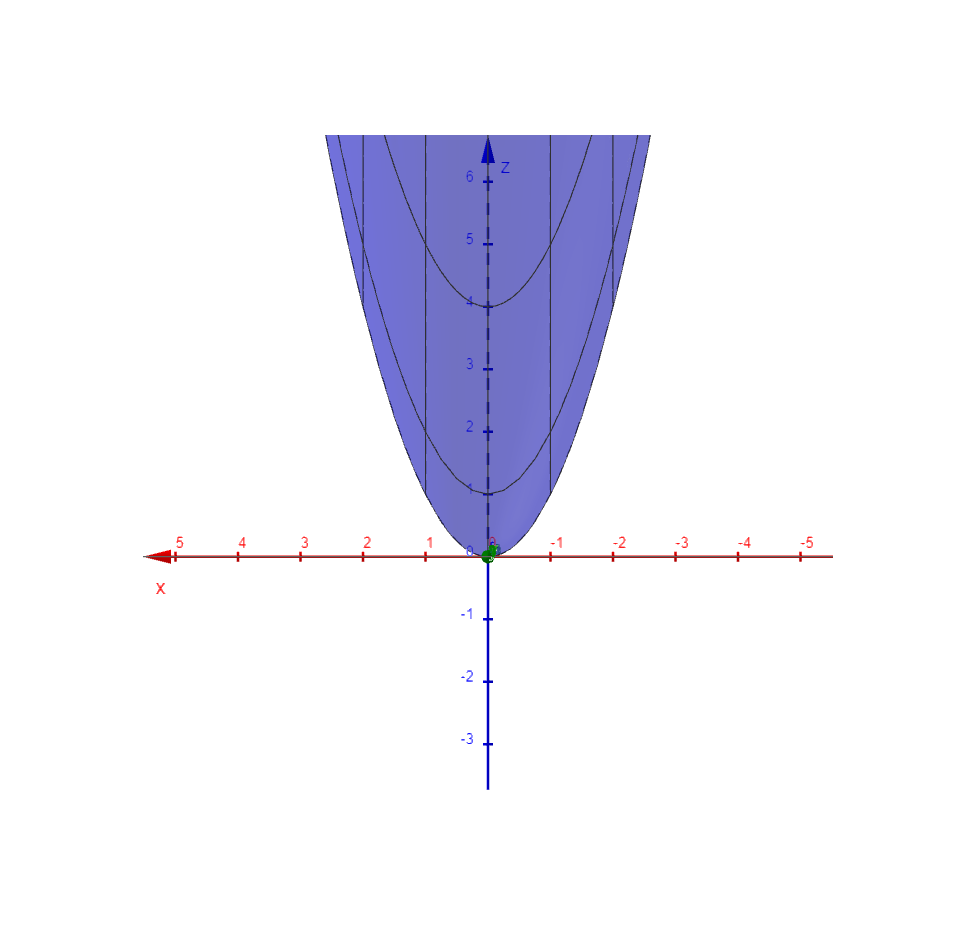
\includegraphics[width=\textwidth]{Capitoli/Capitolo2/Minimo.png}
            \caption{Grafico di $f(x,y)=x^2+y^2$ che mostra un minimo in $(0,0)$.}
        \end{minipage}
        \hspace{1cm}
        \begin{minipage}{0.26\textwidth}
            \centering
            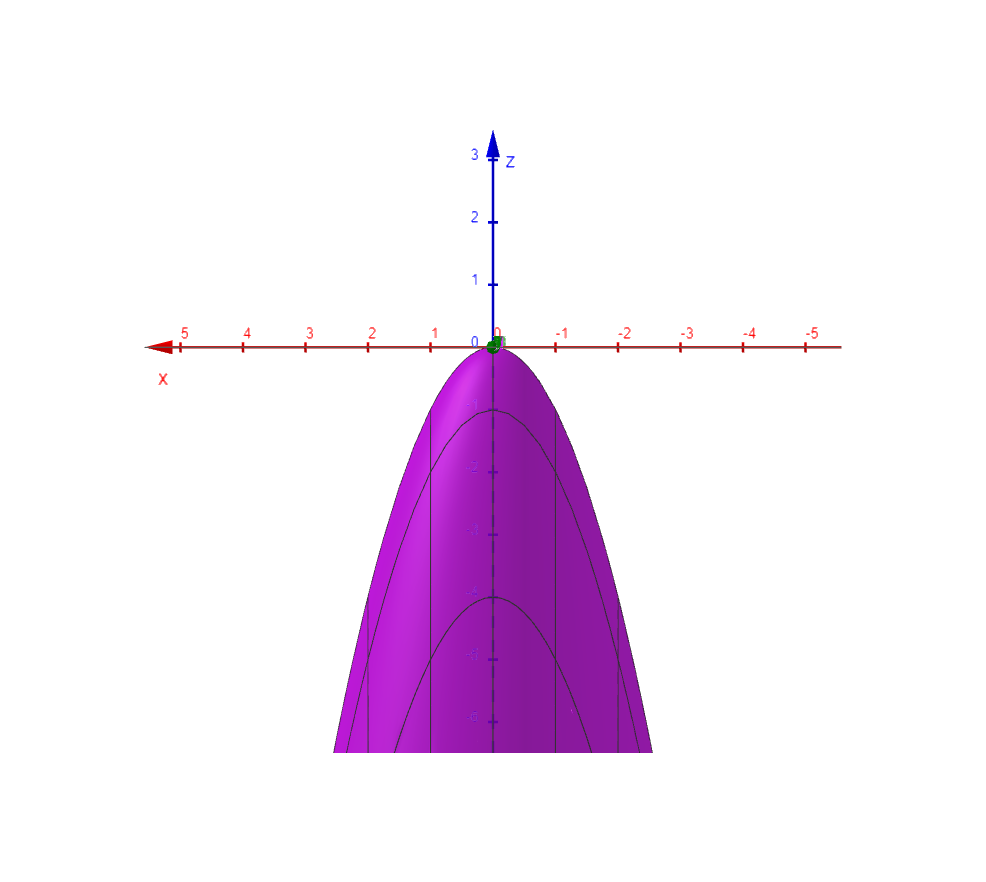
\includegraphics[width=\textwidth]{Capitoli/Capitolo2/Massimo.png}
            \caption{Grafico di $f(x,y)=-x^2-y^2$ che mostra un massimo in $(0,0)$.}
        \end{minipage}
        \hspace{1cm}
        \begin{minipage}{0.26\textwidth}
            \centering
            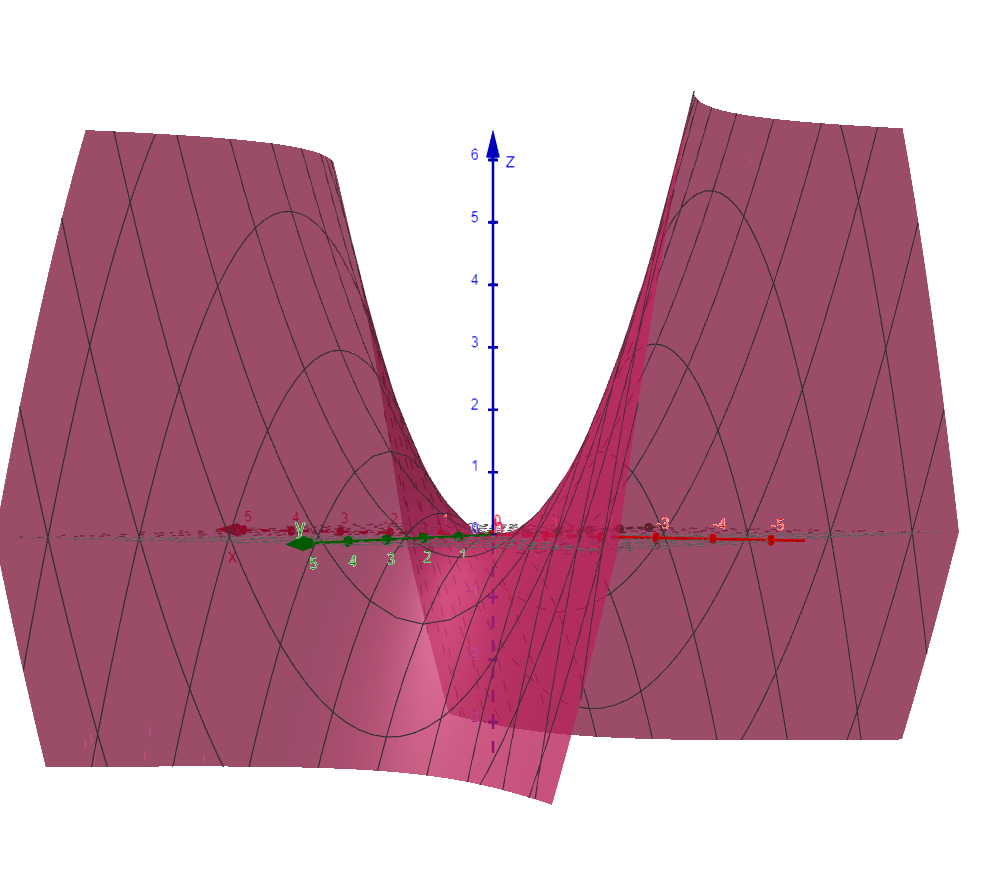
\includegraphics[width=\textwidth]{Capitoli/Capitolo2/Sella 3.png}
            \caption{Grafico di $f(x,y)=\frac{x^2}{3}-\frac{y^2}{3}$ che mostra punto di sella in $(0,0)$.}
        \end{minipage}
    \end{figure}
\end{example}
\paragraph{Richiami sulle forme quadratiche} Una \textbf{forma quadratica} è un polinomio omogeneo di secondo grado tale che
\begin{equation}
    q(\lambda x)=\lambda^2 q(x)\ \forall x \in \mathbb{R}^n,\ \lambda \in \mathbb{R}
\end{equation}
In particolare ad una forma quadratica può essere associata univocamente una matrice rappresentativa simmetrica definita come 
\begin{equation}
    Q=q_{ij}\ \text{con}\ q_{ij}=\frac{a_{ij}+a_{ji}}{2}
\end{equation}
tale che
\begin{equation}
    q(x)=\langle Qx, x \rangle
\end{equation}
\begin{oss}
    Si può notare come nel teorema di Taylor la forma $\langle H_f(x_0)h, h \rangle$ sia una forma quadratica \textit{indotta} da $H_f$.
\end{oss}
Inoltre, una forma quadratica può essere detta:
\begin{itemize}
    \item \textit{Definita positiva (negativa)} se $\forall\ \lambda_i$ si ha che $\lambda_i \underset{(<)}{>}0$
    \item \textit{Semidefinita positiva (negativa)} se $\forall\ \lambda_i$ si ha che $\lambda_i \underset{(\leq)}{\geq}0$
    \item \textit{Indefinita} se $\exists\ \lambda_i, \lambda_j$ tali che $\lambda_i\lambda_j<0$
\end{itemize}
\paragraph{Classificazione dei punti critici} Sia $x_0 \in A$ un punto critico per $f:A \subseteq \mathbb{R}^n\to \mathbb{R}$. Allora il polinomio di Taylor con resto di Peano al secondo ordine è
\begin{equation}
    \begin{aligned}
        f(x_0+h)&=f(x_0)+ \langle \nabla f(x_0), h\rangle+ \frac{1}{2}\langle H_f(x_0)h,h \rangle +o(|h|^2)=\\ 
        &= f(x_0)+ \frac{1}{2}\langle H_f(x_0)h,h \rangle + o(|h|^2)
    \end{aligned}
\end{equation} 
Quindi, per poter fornire dei criteri di classificazione dei punti critici occorre studiare il segno della forma quadratica indotta da $H_f$.
\begin{proposition}
    Sia $f:A \subseteq \mathbb{R}^n \to \mathbb{R}$ e sia $f \in C^2(A)$. Sia poi $x_0$ un punto critico per $f$.\\
    Se $x_0$ è un massimo relativo, allora $H_f(x_0)$ è (semi)definita negativa.
    \begin{equation}
        \langle H_f(x_0)h, h \rangle \underset{(\leq)}{<} 0
    \end{equation}
    Se $x_0$ è un minimo relativo, allora $H_f(x_0)$ è (semi)definita positiva.
    \begin{equation}
        \langle H_f(x_0)h, h \rangle \underset{(\geq)}{>} 0
    \end{equation}
\end{proposition}
\begin{theorem} [Condizione necessaria del II ordine] \label{Teo: Condizione necessaria del secondo ordine}
Sia $f: A \subseteq \mathbb{R}^n \to \mathbb{R}$ e sia $x_0 \in A$ critico per $f$. Sia poi $f \in C^2(A)$. Se $x_0$ è massimo (minimo) relativo, allora $H_f(x_0)$ è semidefinita negativa (positiva).
\end{theorem}
\begin{proof}
    Sia $x_0$ un punto di massimo relativo per $f$ , sia $v \in \mathbb{R}^n$ direzione fissata. Si definisca allora
    \begin{equation}
    F(t)=f(x_0+tv)
    \end{equation}
    Siccome $A$ è aperto, $F$ è definita su un certo $\left(-\delta, \delta\right)$ con $\delta>0$. Per ipotesi su $f$, $F$ ha un massimo relativo in $t=0$ ed è di classe $C^2(-\delta, +\delta)$.\\
    Per l'equazione \eqref{Eq: Premessa al teo Lagrange}, si ottiene che
    \begin{equation}
        F''(t)= \langle H_f(x_0+tv)v, v \rangle 
    \end{equation}
    da cui, per condizione necessaria sulle funzioni di una variabile, segue che
    \begin{equation}
        F''(0)= \langle H_f(x_0)v, v \rangle \leq 0
    \end{equation}
    cioè che $H_f(x_0)$ è semidefinita negativa.\\
    La dimostrazione del caso in cui $x_0$ è minimo relativo per $f$ è del tutto analoga.
\end{proof}
\begin{lemma} \label{Lemma: FQ di matrice simmetrica è compresa tra i suoi autovalori max e min}
        Se, presa $A \in \mathbb{M}_{n,n}$ simmetrica e detti $\lambda_1 \leq \lambda_2 \leq \lambda_n$ i suoi autovalori, si ha $\langle Ax, x \rangle$, allora $\lambda_1 |x|^2 \leq \langle Ax, x \rangle \leq \lambda_n |x|^2$
\end{lemma}
\begin{theorem}[Condizione sufficiente del II ordine] \label{Teo: Condizione sufficiente del secondo ordine}
    Sia $f:A \subseteq \mathbb{R}^n \to \mathbb{R}$ e sia $f \in C^2(A)$. Sia poi $x_0$ un punto critico per $f$. Allora, 
    \begin{itemize}
        \item Se $H_f(x_0)$ è definita positiva (negativa), allora $x_0$ è un minimo (massimo) relativo.
        \item Se $H_f(x_0)$ è indefinita, allora $x_0$ è un punto di sella.
    \end{itemize}
\end{theorem}
    \begin{proof}
        Si consideri il caso in cui $H_f(x_0)$ sia definita positiva e si mostri che $x_0$ è un punto di minimo per $f$\\
        Si può osservare che, essendo $f \in C^2(A)$, allora $H_f$ è simmetrica per il teorema \ref{Teo: Schwarz} e vale dunque il lemma \ref{Lemma: FQ di matrice simmetrica è compresa tra i suoi autovalori max e min}. Pertanto, indicato con $\lambda_{min}>0$ il minor autovalore di $H_f$, si ha che
        \begin{equation}
            \langle H_f(x_0)h,h \rangle \geq \lambda_{min} |h|^2 \qquad \forall h \in \mathbb{R}^n
        \end{equation}
        Si scriva quindi lo sviluppo di Taylor con resto di Peano al secondo ordine in $f(x_0)$.
        \begin{equation}
        \begin{aligned}
            f(x_0+h)-f(x_0)&= \langle \nabla f(x_0), h \rangle + \frac{1}{2}\langle H_f(x_0h, h\rangle + o(|h|^2)=\\
            &\overset{f'(x_0)=0}{=} \frac{1}{2}\langle H_f(x_0)h, h\rangle + o(|h|^2) \geq \\
            &\overset{\text{Lemma}\ \ref{Lemma: FQ di matrice simmetrica è compresa tra i suoi autovalori max e min}}{\geq} \frac{1}{2} \lambda_{min}|h|^2+o(|h|^2)
        \end{aligned}
        \end{equation}
        Poiché scopo della dimostrazione è mostrare che $f(x_0+h)-f(x_0) \geq 0\ \forall h \in \mathbb{R}^n$, occorre provare che $o(|h|^2)$ sia trascurabile.
        \begin{equation}
            f(x_0+h)- f(x_0) \geq \frac{1}{2}\lambda_{min} |h|^2 \left( 1 + \frac{o(|h|^2)}{\tfrac{1}{2}\lambda_{min}|h|^2}\right)
        \end{equation}
        ma, per definizione di o-piccolo vale il seguente fatto:
        \begin{equation}
            \exists\ \sigma >0\ \text{tale che, se}\ |h|<\sigma\ \text{allora}\ \left|\frac{o(|h|^2)}{\tfrac{1}{2}\lambda_{min} |h|^2}\right| < \frac{1}{2}
        \end{equation}
        dove $\sigma=\frac{1}{2}$ è una costante arbitraria in $(0,1)$.
        Per tale disuguaglianza, allora, 
        \begin{equation}
        \begin{aligned}
            f(x_0+h)-f(x_0)&\geq \frac{1}{2}\lambda_{min} |h|^2 \left( 1 + \frac{o(|h|^2)}{\tfrac{1}{2}\lambda_{min}|h|^2}\right) \geq \\
            &\geq \frac{1}{2}\lambda_{min}|h|^2\left(1-\frac{1}{2}\right)=\frac{1}{4}\lambda_{min}|h|^2 >0
            \end{aligned}
        \end{equation}
        purché $|h|< \sigma$. In tal caso la definizione di minimo è soddisfatta.\\
        La dimostrazione per $H_f(x_0)$ definita negativa è analoga.\\
    Si dimostri ora il punto 2.\\
    Se $H_f(x_0)$ è indefinita, allora non soddisfa le ipotesi della condizione necessaria del secondo ordine (teorema \ref{Teo: Condizione necessaria del secondo ordine}), cioè non è né massimo né minimo. Quindi, essendo per ipotesi critico, deve essere una sella.
    \end{proof}
    \begin{oss}
        Se vale $f(x_0+h)-f(x_0) \gtrless 0$, $x_0$ si dice minimo (massimo) forte.
    \end{oss}
    \begin{oss}
        Si noti che non è possibile concludere niente previa indagine nel caso in cui $H_f$ sia semidefinita.
    \end{oss}
    \paragraph{Metodo delle restrizioni} Come accennato, se $H_f(x_0)$ è semidefinita, non è possibile caratterizzare il punto critico. Si mostri allora un metodo per farlo tramite esempio.
    \begin{example}
        Sia $f(x,y)=x^4-y^4$. Allora il punto $(0,0)$ è critico e si ha che
        \begin{equation*}
            H_f(0,0)=\begin{pmatrix}
                0 & 0\\
                0 & 0
            \end{pmatrix}
        \end{equation*}
        con $f(0,0)=0$. Si può osservare, però che:
        \begin{equation*}
            \begin{aligned}
                &f(x, 0) > 0 \qquad \forall x \neq 0\\
                &f(0,y) < 0 \qquad \forall y \neq 0
            \end{aligned}
        \end{equation*}
        Pertanto $(0,0)$ è un punto di sella, giacché non è né un massimo né un minimo.
    \end{example}
    Può capitare, però, di non trovare restrizioni di quel genere, allora bisogna ricorrere allo studio del segno di
    \begin{equation*}
        f(x)-f(x_0)
    \end{equation*}
\section{Funzioni a valori vettoriali}
\begin{definition} \label{Def: Funzioni a valori vettoriali}
    Siano $n,\ m \in \mathbb{N}$ e sia $A \subseteq \mathbb{R}^n$. Allora si dice che una funzione $f$ è \textbf{a valori vettoriali} se è così definita:
    \begin{equation}
    \begin{aligned}
        f:A \subseteq \mathbb{R}^n &\to \mathbb{R}^m\\
        (x_1, \dots, x_n) &\mapsto (f_1(x_1, \dots, x_n), \dots, f_n(x_1, \dots, x_n))
    \end{aligned}
    \end{equation}
\end{definition}
\begin{oss}
    Si noti che limiti, continuità e derivabilità vanno estese ad un ragionamento componente per componente.
\end{oss}
\begin{oss}
    Se la dimensione del dominio e del codominio è la medesima, si parla di \textit{campo vettoriale}.
\end{oss}
\begin{definition} \label{Def: Derivabilità di f. vettoriali}
    Si dice che $f:A \subseteq \mathbb{R}^n \to \mathbb{R}^m$ è \textbf{derivabile} in $x_0 \in A$ se ciascuna $f_i$ con $i=1, \dots, n$ è ivi derivabile.
\end{definition}
\begin{definition} \label{Def: Matrice Jacobiana}
    Se $f$ è derivabile in $x_0$, si dice \textbf{matrice jacobiana} di $f$ in $x_0$ la matrice $J_f \in \mathbb{M}_{m,n}$ definita da
    \begin{equation} \label{Eq: Matrice Jacobiana}
        J_f(x_0)=\begin{pmatrix}
            \frac{\partial{f_1}}{\partial{x_1}}(x_0) & \frac{\partial{f_1}}{\partial{x_2}}(x_0)& \dots & \frac{\partial{f_1}}{\partial{x_n}}(x_0)\\
            \frac{\partial{f_2}}{\partial{x_1}}(x_0)& \frac{\partial{f_2}}{\partial{x_2}}(x_0)& \dots & \frac{\partial{f_2}}{\partial{x_n}}(x_0)\\
            \vdots & \vdots & \ddots & \vdots\\
            \frac{\partial{f_n}}{\partial{x_1}}(x_0) & \frac{\partial{f_n}}{x_2}(x_0)& \dots & \frac{\partial{f_n}}{\partial{x_n}}(x_0)
        \end{pmatrix}
        =
        \begin{pmatrix}
            \nabla f_1 (x_0)\\
            \nabla f_2(x_0)\\
            \vdots\\
            \nabla f_n(x_0)
        \end{pmatrix}
    \end{equation}
    Il determinante della matrice Jacobiana è detto \textbf{Jacobiano} \label{Def: Jacobiano}
\end{definition}
\begin{definition} \label{Def: Differenziabilità di f. vettoriali}
    Una funzione $f$ si dice \textbf{differenziabile} in $x_0 \in A$ se
    \begin{equation}
        \lim_{h \to 0}{\frac{f(x_0+h)-f(x_0)-J_f(x_0)h}{|h|}}=0
    \end{equation}
\end{definition}

\begin{theorem} \label{Teo: Derivata composta di f. vettoriali}
Siano $g: B \subseteq \mathbb{R}^k \to A \subseteq R^n$ e $f: A \subseteq \mathbb{R}^n \to \mathbb{R}^m$ e le si assuma di classe $C^1$. Allora, $h=f \circ g: B \to \mathbb{R}^m$ è ben definita su $B$, è di classe $C^1(B)$ e vale:
\begin{equation}
    J_h(y) \in \mathbb{M}_{m,n}\ \text{tale che}\ J_h(y)=J_f(g(y)) J_g(y) \qquad \forall\ y \in B
\end{equation}
\end{theorem}
\begin{oss}
    Essendo di classe $C^1$, $h$ è differenziabile, in accordo con i ragionamenti già svolti nell'equazione \eqref{Eq: Relazione C^1 -> diff -> C^0}.
\end{oss}\cleardoublepage
\chapter{Funzioni implicite}
\section{Introduzione alle funzioni implicite}
Può spesso capitare di avere a che fare con insiemi di $\mathbb{R}^2$ descritti da
\begin{equation} \label{Eq: Insieme implicito}
    F(x,y)=0 
\end{equation}
e detti \textbf{impliciti}.\\
L'obiettivo del capitolo è quello di trovare le condizioni sotto le quali la \eqref{Eq: Insieme implicito} permetta di associare ad $x$ un unico valore di $y$ come funzione di $x$,  arrivando a determinare le condizioni di esistenza di un intervallo $I \subseteq \mathbb{R}^n$ e di una funzione $f: I \to \mathbb{R}$ tale che
\begin{equation} \label{Eq: Scopo capitolo 3}
    F(x, f(x))=0 \qquad \forall\ x \in I
\end{equation}
Prima di procedere nella trattazione, si forniscano alcune definizioni di base utili nel corso del capitolo.
\begin{definition} \label{Def: Funzione implicita}
    Siano $I \subseteq \mathbb{R}^2,\ J \subseteq \mathbb{R}$ tali che
    \begin{equation}
        \forall\ x\in I\ \exists!\ y \in J\ \text{tale che}\ F(x,y)=0
    \end{equation}
    Allora si dice che l'equazione $F(x,y)=0$ \textbf{definisce implicitamente} una funzione $f: I \to J$.
\end{definition}
\begin{definition} \label{Def: Insieme degli zeri}
    Si dice \textbf{insieme degli zeri} della funzione $F$ l'insieme $Z(F)$ così definito:
    \begin{equation} \label{Eq: Insieme degli zeri}
        Z(F)=\left\{(x,y) \in I \mid F(x, y)=0 \right\}
    \end{equation}
\end{definition}
\begin{definition}
    Sia $Z(F)$ definito come nella \eqref{Eq: Insieme degli zeri} e sia $P=(\overline{x}, \overline{y}) \in Z(F)$. Se $\nabla F(\overline{x}, \overline{y})\neq 0$, si dice che $P$ è un \textbf{punto regolare} di $Z(F)$. Altrimenti $P$ è un \textbf{punto singolare}.
\end{definition}
\section{Teorema del Dini}
Il teorema del Dini, che verrà affrontato di seguito, fornisce le condizioni sotto le quali l'equazione $F(x,y)=0$ esprime $y$ in funzione di $x$ per certi valori delle variabili $x$, $y$.
\newpage
\begin{theorem}[Teorema del Dini] \label{Teo: Teorema del Dini}
    Sia $F: A \subseteq \mathbb{R}^2 \to \mathbb{R}$, $A$ aperto, una funzione continua in A e tale che
    \begin{equation}
    \exists\ \frac{\partial{F}}{\partial{y}} \in A 
    \end{equation}
    ed essa sia ivi continua. Inoltre, preso $(x_0, y_0) \in A$, se 
    \begin{equation}
    (x_0, y_0) \in Z(F) \quad \text{e} \quad \frac{\partial{F}}{\partial{y}}(x_0, y_0) \neq 0
    \end{equation}
    Allora, l'equazione
    \begin{equation}
        F(x, y)=0
    \end{equation}
    definisce implicitamente un'unica funzione
    \begin{equation}
        g: (x_0-\delta, x_0+\delta) \to (y_0 - \sigma, y_0+\sigma)
    \end{equation}
    tale che 
    \begin{equation} \label{Eq: Tesi Dini}
     y=g(x) \iff
        \begin{cases}
            F(x, y)=0\\
            x \in (x_0-\delta, x_0+\delta)\\
            y \in (y_0 - \sigma, y_0+\sigma)
        \end{cases} 
    \end{equation}
    Inoltre $g$ è continua in $(x_0-\delta, x_0+\delta)$ e $g(x_0)=y_0$
\end{theorem}
\begin{proof}
        Si supponga $\frac{\partial{F}}{\partial{y}}(x_0,y_0) > 0$. Poiché per ipotesi essa è anche continua, per permanenza del segno si ha che $\exists\ \sigma > 0$ tale che
        \begin{equation}
            \frac{\partial{F}}{\partial{y}}(x,y) > 0 \quad \forall\ (x,y) \in [x_0-\sigma, x_0+\sigma]\times [y_0 - \sigma, y_0+\sigma]
        \end{equation}
       Sia $x_0$ fissato. Definita $\eta(y)=F(x_0, y)$ si ha che
       \begin{equation}
           \eta'(y)=\frac{\partial{F}}{\partial{y}}(x_0, y) >0 \quad \forall\ y \in [y_0 - \sigma, y_0+\sigma]
       \end{equation}
       Pertanto $\eta(y)$ è continua, strettamente crescente e nulla in $y_0$. Quindi
       \begin{equation}
       \begin{aligned}
           &\eta(y_0-\sigma)=F(x_0, y_0-\sigma)<0\\
           &\eta(y_0+\sigma)=F(x_0, y_0+\sigma)>0
       \end{aligned}
       \end{equation}
       Allora, per permanenza del segno su $F$, $\exists\ \delta>0,\ \delta \leq \sigma$ tale che 
       \begin{equation}
           F(x, y_0-\sigma) < 0 < F(x, y_0+\sigma) \quad \forall x \in [x_0-\delta, x_0+\delta]
       \end{equation}
       Dunque, per ogni $\overline{x} \in [x_0-\delta, x_0+\delta]$ fissato, la funzione $\eta_{\overline{x}}(y)=F(\overline{x}, y)$ è monotona, strettamente crescente, di segno opposto agli estremi di $[y_0 - \sigma, y_0+\sigma]$. Quindi, per il teorema dei valori intermedi, si sa che $\forall \overline{x} \in [x_0-\delta, x_0+\delta]$ esiste un unico $\overline{y} \in [y_0-\sigma, y_0+\sigma]$ tale che 
       \begin{equation}
           F(\overline{x}, \overline{y})=0
       \end{equation}
       Allora, definito $\overline{y}=g(\overline{x})$ si ha, per costruzione, la dimostrazione di \eqref{Eq: Tesi Dini} e di $g(x_0)=y_0$.\\
       Rimane da mostrare la continuità di $g$.
       \begin{equation}
           \forall\ \varepsilon > 0\ \exists\ \xi > 0\ \text{tale che, se}\ |x-\overline{x}|< \xi\ \text{allora}\ |g(x)-g(\overline{x})| < \varepsilon
       \end{equation}
       Per quanto dedotto prima, cioè $F(\overline{x}, g(\overline{x}))=0$ e $\frac{\partial{F}}{\partial{y}}>0$, si sa che 
       \begin{equation}
           F(\overline{x}, g(\overline{x})-\varepsilon)<0<F(\overline{x}, g(\overline{x})+\varepsilon)
       \end{equation}
       In maniera analoga, per permanenza del segno, si ha che per ogni $x \in (\overline{x}-\xi, \overline{x}+\xi)$ vale
       \begin{equation}
           F(x, g(\overline{x})-\varepsilon)<0<F(x, g(\overline{x})+\varepsilon)
       \end{equation}
       Poiché infine $F(x, g(x))=0\ \forall\ x \in (\overline{x}-\xi, \overline{x}+\xi)$ e $F$ è crescente in tutti i punti considerati,
       \begin{equation}
           g(\overline{x})- \varepsilon < g(x) < g(\overline{x})+\varepsilon
       \end{equation}
       cioè $g$ continua in $\overline{x}$.
       \end{proof}
\begin{oss}
    Il teorema offre solo una condizione sufficiente, infatti, presa $G(x,y)=(F(x,y))^2$, da una parte si ha $Z(G)=Z(F)$ ma, dall'altra, $\nabla G \big|_{Z(G)}=0$.
\end{oss}
\begin{theorem}[Derivata delle funzioni implicite]
Siano le ipotesi del Dini con in aggiunta $F \in C^1(A)$, allora anche $g \in C^1(U)$ e la derivata $g'$ vale
\begin{equation}
    g'(x)=-\frac{\frac{\partial{F}}{\partial{x}}(x, g(x))}{\frac{\partial{F}}{\partial{y}}(x, g(x))} \qquad \forall\ x \in U=[x_0-\delta, x_0+\delta]
\end{equation}
\end{theorem}
\begin{proof}
Sia $(\xi, \eta) \in \left[(x, g(x)), (x+h, g(x+h)) \right]$.
Si scriva il teorema di Lagrange per $F$.
\begin{equation}
    F(x+h, g(x+h))-F(x, g(x)) =\langle \nabla F (\xi, \eta), (h, [g(x+h)-g(x)]) \rangle
\end{equation}
Svolgendo il prodotto scalare e sfruttando le ipotesi del Dini si ha che
\begin{equation}
    F(x+h, g(x+h))-F(x, g(x))= \frac{\partial {F}}{\partial{x}}(\xi, \eta) h + \frac{\partial {F}}{\partial{y}}(\xi, \eta) (g(x+h)-g(x))=0
\end{equation}
    Da ciò quindi si ottiene che
    \begin{equation}
        \lim_{h \to 0}{\frac{g(x+h)-g(x)}{h}}=\lim_{h \to 0}{-\frac{\frac{\partial {F}}{\partial{x}}(\xi, \eta)}{\frac{\partial {F}}{\partial{y}}(\xi, \eta)}}
    \end{equation}
Essendo $F \in C^1$ ne consegue che $g$ è derivabile in $U$ e, essendo continue per ipotesi le derivate parziali, si ha proprio che
\begin{equation}
    g'(x)=-\frac{\frac{\partial{F}}{\partial{x}}(x, g(x))}{\frac{\partial{F}}{\partial{y}}(x, g(x))} \qquad \forall\ x \in U
\end{equation}
\end{proof}
\begin{corollary}
    Valgano le ipotesi del teorema del Dini con, in aggiunta, $F \in C^k(A),\ k \in \mathbb{N}$. Allora $g \in C^k(U)$.
\end{corollary}
\begin{proof}
    Si svolga la dimostrazione per induzione.
    Nel caso base in cui $k=0$, ciò è vero per quanto visto. Stesso dicasi per $k=1$. Allora si supponga l'enunciato vero per $k-1$ e si provi che è vero per $k$, preso $k>2$.\\
    Se $F \in C^k(A)$, allora $F \in C^{k-1}$ e, per ipotesi induttiva, $g \in C^{k-1}(U)$. Allora, 
    \begin{equation}
         g'(x)=-\frac{\frac{\partial{F}}{\partial{x}}(x, g(x))}{\frac{\partial{F}}{\partial{y}}(x, g(x))} \in C^{k-1}
    \end{equation}
    cioè, $g \in C^k(U)$
\end{proof}
È possibile, tali premesse calcolare anche la derivata seconda di $g$. Infatti gli ultimi due risultati permettono di calcolare la derivata prima di $g$ e garantiscono che se $F \in C^2(A)$, allora $g \in C^2(U)$, quindi si formalizzi il calcolo della derivata seconda di $g$.
\begin{theorem}[Derivata seconda delle funzioni implicite]
Sia $F \in C^2(A)$. Allora $g \in C^2(U)$ e
\begin{equation}
    g''(x)= \left(\frac{-F_{xx}F_{y}^2+2F_{xy}F_xF_y-F_{yy}F_x^2}{F_y^3}\right)(x, g(x))
\end{equation}
\end{theorem}
\begin{proof}
Essendo $F$ di classe $C^2$, e sapendo che $F(x,g(x))=0$, si derivi a destra e sinistra.
\begin{equation}
    \frac{\partial{F}}{\partial{x}}(x, g(x))+\left(\frac{\partial{F}}{\partial{y}}(x, g(x)\right)g'(x)=0
\end{equation}
Derivando un'altra volta si scopre che
\begin{equation}
    \frac{\partial^2{F}}{\partial{x^2}}(x, g(x))+ 2 \frac{\partial^2{F}}{\partial{x}\partial{y}}(x, g(x))g'(x) + \frac{\partial^2{F}}{\partial{y^2}}(x, g(x))(g'(x))^2+ \frac{\partial{F}}{\partial{y}}g''(x) =0
\end{equation}
e quindi, esplicitando $g''$
\begin{equation}
\begin{aligned}
    g''(x)&= \left(\frac{-F_{xx}-2F_{xy}g'(x)- F_{yy}g'(x)^2}{F_y}\right)(x, g(x))=\\
    &\overset{g'(x)=-\tfrac{F_x}{F_y}}{=} \left(\frac{-F_{xx}F_{y}^2+2F_{xy}F_xF_y-F_{yy}F_x^2}{F_y^3}\right)(x, g(x))
\end{aligned}
\end{equation}
\end{proof}
\begin{oss}
    Se $F \in C^2(A)$ la condizione sufficiente affinché un punto $x_0$ sia massimo per $g$ è che
    \begin{equation}
        \begin{aligned}
            &g'(x_0)=0 \Rightarrow\ F_x(x_0, g(x_0))=0\\
            &g''(x_0)<0 \Rightarrow\ -\frac{F_{xx}(x_0, g(x_0))}{F_y} < 0
        \end{aligned}
    \end{equation}
\end{oss}
\begin{example}
    Si mostri un esempio pratico sulle applicazioni dei teoremi visti.\\
    Sia $F(x,y)=x \log y - y \cos x$. Si mostri che $F\left(\tfrac{\pi}{2}, 1\right)$ definisce implicitamente un'unica funzione $g \in C^\infty$ tale che $y=g(x)$ e se ne determini lo sviluppo di Taylor al secondo ordine. 
    \begin{enumerate}
        \item Si controlli che $F\left(\tfrac{\pi}{2}, 1\right)=0$.\\
        Ciò è vero, poiché $F\left(\tfrac{\pi}{2}, 1\right)=\tfrac{\pi}{2} \log 1 - \cos\left(\tfrac{\pi}{2}\right)=0$.
        \item Si osservi che, siccome $F \in C^\infty$, se esiste una $g$, deve essere anch'essa di classe $C^\infty$.
        \item Si verifichi che $F_y(\tfrac{\pi}{2}, 1) \neq 0$.\\
        $\nabla F(x, y) = (\log y + y \sin{x}, \tfrac{x}{y}- \cos{x}) \Rightarrow F_y(\tfrac{\pi}{2},1)=\tfrac{\pi}{2}$
        \item Verificate tali condizioni, per il teorema del Dini, esiste una $g(x)=y$ tale che $g(\tfrac{\pi}{2})=1$. Per calcolarne lo sviluppo occorre ricavare mediante le formule ottenute prima $g'(\tfrac{\pi}{2})$ e $g''(\tfrac{\pi}{2})$.
        \item Infine, $g(x)=g\left(\tfrac{\pi}{2}\right) + g'\left(\tfrac{\pi}{2}\right)\left(x-\tfrac{\pi}{2}\right)+ \tfrac{g''\left(\tfrac{\pi}{2}\right)}{2}\left(x-\tfrac{\pi}{2}\right)^2+ o\left(\left(x-\tfrac{\pi}{2}\right)^2\right)$
    \end{enumerate}
\end{example}
\begin{theorem}[Ortogonalità del gradiente alle curve di livello] \label{Teo: Ortogonalità del gradiente alle curve di livello}
    Sia $F: A \subseteq \mathbb{R}^2 \to \mathbb{R}$ tale che $F \in C^1(A)$. Supponendo $(x_0,y_0) \in Z(F)$ e $\nabla F \neq (0,0)$ in $Z(F)$, si ottiene che $\nabla F(x_0,y_0) \perp Z(F)$ in $(x_0, y_0)$.\\Preso $\mathcal{L}_a$ insieme di livello $a$ e considerata $G(x,y)=F(x,y)-a$, il teorema vale sugli insiemi di livello in generale.
\end{theorem}
\begin{proof}
    Per il teorema del Dini, $Z(F)$ in un intorno di $(x_0, y_0)$ è il grafico di una funzione implicita $g: (x_0- \delta, x_0+ \delta) \to \mathbb{R}$. In particolare esso è il sostegno della curva parametrica $\gamma = (x, g(x))$. Il versore tangente di $\gamma$ è dunque definito da
    \begin{equation}
        T(x)= \frac{(1, g'(x))}{\sqrt{1+g'(x)^2}} \qquad x \in (x_0- \delta, x_0+ \delta)
    \end{equation}
    Calcolando per tali valori di $x$ il prodotto scalare tra il gradiente ed il versore tangente si ha che
    \begin{equation}
        \langle \nabla F (x, g(x)), T(x) \rangle= \frac{F_x(x, g(x)) + F_y(x, g(x))g'(x)}{\sqrt{1+g'(x)^2}}=\frac{F'(x, g(x))}{\sqrt{1+g'(x)^2}}=0
    \end{equation}
    cioè la tesi.
\end{proof}

Bisogna anche ricordare che il teorema del Dini può essere applicato anche in altri contesti oltre a quanto già visto. Infatti, esiste una versione del teorema applicata alle funzioni di più variabili ed un'altra applicata ai sistemi di equazioni, di cui si riporta solo l'enunciato.
\begin{theorem}[Teorema del Dini per le funzioni in più variabili]
Siano $x=(x_1, \dots, x_n) \in \mathbb{R}^n$, $y \in \mathbb{R}$ e sia $F(x, y)=F(x_1, \dots, x_n, y)$ una funzione continua nell'aperto $A \in \mathbb{R}^{n+1}$ insieme alla sua derivata parziale $F_y$ in $A$. Se $(x_0, y_0)=(x_{01}, \dots, x_{0n}, y_0)\in A$ è tale che
\begin{equation}
    F(x_0, y_0)=0 \qquad F_y(x_0, y_0) \neq 0
\end{equation}
allora esistono $\delta, \sigma>0$ ed un'unica funzione $f: B_\delta(x_0) \to (y_0-\sigma, y_0+ \sigma)$ tale che 
\begin{equation}
    F(x, f(x))=0 \qquad \forall x \in B_\delta(x_0)
\end{equation}
\end{theorem}
\begin{theorem}[Teorema del Dini per i sistemi]
    Siano $A \in \mathbb{R}^{n+h}$ un aperto e $F=F(x,y): A \to \mathbb{R}^h$ di classe $C^1$. Sia poi $(x_0, y_0) \in A$ tale che
    \begin{equation}
        F(x_0, y_0)=0\quad \land \quad \det(J_f) \neq 0
    \end{equation}
    allora esistono un intorno sferico $I$ di $x_0$, un intorno sferico $J$ di $y_0$ ed un'unica funzione $f: I \subset \mathbb{R}^n \to J \subset\mathbb{R}^h$. tale che $f(x_0)=y_0$
    \begin{equation}
        F(x, f(x))=0 \qquad \forall x \in I
    \end{equation}
\end{theorem}
Si può inoltre notare che una conseguenza del teorema del Dini è il teorema delle funzioni inverse in una variabile reale. In realtà, tale risultato può essere ampliato alle funzioni di più variabili sfruttando il concetto di invertibilità locale.
\begin{definition} \label{Def: Invertibilità locale}
    Sia $f: A \subseteq \mathbb{R}^n \to \mathbb{R}$ con $f \in C^1(A)$. Allora essa è detta \textbf{localmente invertibile} in $x_0 \in A$ se esiste un intorno $B_\delta(x_0) \subseteq A$ tale che la restrizione di $f$ a $B_\delta$, cioè $f\big|_{B_\delta(x_0)}$, sia una funzione invertibile di $B$ su $f(B_\delta)$.
\end{definition}
Tale nozione può essere potenziata definendo poi i diffeomorfismi locali.
\begin{definition} \label{Def: Diffeomorfismo}
    Sia $f$ localmente invertibile e definita su $f(B_\delta(x_0))$ aperto e siano $f$ e la sua inversa entrambe di classe $C^1$ nei propri domini, allora $f$ si dice $\mathbf{C^1}$\textbf{-diffeomorfismo}
\end{definition}
\begin{theorem}[Invertibilità locale] \label{Teo: Invertibilità locale}
    Sia $A \subseteq \mathbb{R}^n$ e $f: A \to \mathbb{R}^n$ una funzione di classe $C^1(A)$. Allora se $x_0 \in A$ è tale che lo Jacobiano (\ref{Def: Jacobiano})in $x_0$ sia non nullo, cioè $\det(J_f(x_0) \neq 0$, esistono $B_\delta(x_0)$ aperto e $J$, intorno aperto di $f(x_0)$ tali che la funzione $f\big|_{B_\delta(x_0)}: B_\delta(x_0) \to J$ è invertibile con inversa $f^{-1}: J \to B_\delta(x_0)$ di classe $C^1$. Inoltre, 
    \begin{equation}
        J_{f^{-1}}(y)=(J_f(f^{-1}(y)))^{-1}
    \end{equation}
\end{theorem}
\section{Ottimizzazione vincolata}
Dopo aver descritto le funzioni implicite, può essere utile capire come queste possano essere massimizzate o minimizzate lungo un determinato vincolo.
\begin{definition} \label{Def: Vincolo di uguaglianza}
Sia F una funzione di classe $C^1$. Si dice \textbf{vincolo di uguaglianza} un insieme $V \subseteq \mathbb{R}^n$ della forma
\begin{equation}
    V= \left\{(x_1, \dots, x_n) \in \mathbb{R}^n \mid F(x_1, \dots, x_n)=0 \right\}
\end{equation}
\end{definition}
Presa dunque una funzione $f:A\subseteq \mathbb{R}^n \to \mathbb{R}$ con $V \subseteq A$, occorre verificare l'esistenza ed eventualmente determinare $\min\limits_{V}{f}$ e $\max\limits_{V}{f}$.
In particolare, si affronterà il caso con $n=2$.
\begin{definition} \label{Def: Estremi vincolati}
    Un punto $(x_0, y_0) \in V= Z(F)$ con $F \in C^1$ è detto \textbf{punto di massimo (minimo) relativo vincolato} per $f$ su $Z(F)$ se esiste $\delta>0$ tale che 
    \begin{equation}
        f(x,y) \underset{(\geq)}{\leq} f(x_0, y_0) \qquad \forall\ (x, y) \in B_\delta(x_0, y_0) \cap Z(F)
    \end{equation}
    In tal caso $(x_0, y_0)$ è detto \textbf{estremo relativo vincolato}.\\
    Poi, $(x_0, y_0)$ è detto \textbf{punto di massimo (minimo) assoluto} per $f$ su $Z(F)$ se vale
    \begin{equation}
        f(x, y) \underset{(\geq)}{\leq} f(x_0, y_0) \qquad \forall\ (x, y) \in Z(F)
    \end{equation}
    Infine, i valori nei punti di massimo (minimo) sono detti \textbf{massimo (minimo)} della funzione.
\end{definition}
\begin{definition} \label{Punto critico vincolato}
    Siano $f \in C^1,\ F \in C^1$ definite come sopra e sia $(x_0, y_0) \in Z(F)$. Indicato con $\tau$ il versore tangente a $Z(F)$ in $(x_0, y_0)$, si dice che $(x_0, y_0)$ è un \textbf{punto critico vincolato} per $f$ su $Z(F)$ se la sua \textbf{derivata tangenziale} al vincolo di $f$ in tale punto è nulla, cioè:
    \begin{equation} \label{Eq: Derivata tangenziale}
        \frac{\partial{F}}{\partial \tau}(x_0, y_0)=0 
    \end{equation}
\end{definition}
\paragraph{Determinare gli estremi vincolati lungo un vincolo esplicitabile}
È possibile sviluppare dei metodi per individuare eventuali estremi vincolati. Si prenda in considerazione il caso in cui il vincolo sia dato da una curva.
Sia $V$ dato come curva parametrica $(x(t), y(t))$ con $t \in \mathbb{R}$ di classe $C^1$.
In tal caso $f \big|_V$ è data da $h(t)=f(x(t), y(t)) \in C^1$. Quindi ci si è ricondotti al caso di funzioni in una variabile. Si può dunque notare che se $(x(t_0), y(t_0))$ è un estremo relativo vincolato per $f$ su $V$, è noto che $h'(t_0)=0$.\\
Inoltre, poiché $h'(t_0)= \langle \nabla f(x(t), y(t)), (x'(t), y'(t)) \rangle \big|_{t_0}=0$, si può affermare che $\nabla f(x(t), y(t)) \perp (x'(t), y'(t))$, cioè che $\nabla f$ è ortogonale alla curva nel punto di estremo.
\begin{theorem}[Moltiplicatore di Lagrange] \label{Teo: Moltiplicatore di Lagrange}
Siano $A \subseteq \mathbb{R}^2$ aperto, $f: A \to \mathbb{R}$ e $F: A \to \mathbb{R}$ tali che entrambe siano di classe $C^1$. Siano poi $Z(F)= \left\{ (x,y) \in A \mid F(x,y)=0\right\}$ e $(x_0,y_0)$ un punto regolare di $Z(F)$. Allora se $(x_0, y_0)$ è un estremo relativo vincolato per $f$ su $Z(F)$, si ha che
\begin{enumerate}
    \item  $\exists\ \lambda_0 \in \mathbb{R}$, detta \textbf{moltiplicatore di Lagrange}, tale che $\nabla f(x_0, y_0)= \lambda_0 \nabla F(x_0, y_0)$.
    \item $(x_0, y_0)$ è un punto critico vincolato per $f$ su $Z(F)$.
    \item $(x_0, y_0)$ è un punto critico libero della Lagrangiana $\mathcal{L}(x, y, \lambda)=f(x,y)- \lambda F(x, y)$.
\end{enumerate}
\end{theorem}
\begin{proof}
    Poiché $(x_0, y_0) \in Z(F)$ è regolare in $Z$, cioè $\nabla F(x_0, y_0) \neq 0$, si ha 
    \begin{equation}
        F_x(x_0, y_0) \neq 0 \lor F_y(x_0, y_0) \neq 0
    \end{equation}
    Si supponga allora, senza perdita di generalità, che la derivata parziale lungo $y$ sia non nulla. Allora, per il teorema del Dini, esistono $U(x_0)$, $V(y_0)$ tali che esista
    \begin{equation}
    h:U(x_0) \to V(y_0) \iff \begin{cases}
        F(x, y)=0\\
        x\in U(x_0)\\
        y \in V(y_0)
    \end{cases}
    \end{equation}
    Inoltre, sempre per il teorema del Dini, è noto che
    \begin{equation} \label{Eq: Derivata implicita per teorema moltiplicatore}
        h'(x)=- \frac{F_x(x_0, y_0)}{F_y(x_0, y_0)} 
    \end{equation}
    Si dimostri quindi il punto 1.\\
    Sia $\mathcal{F}$ così definita:
    \begin{equation}
        \mathcal{F}(x)=f(x, h(x)) \quad x \in U(x_0)
    \end{equation}
    Poiché $x_0$ è interno a $U$ e, per ipotesi, $x_0$ è punto critico per $f$, $\mathcal{F}$ è derivabile in $x_0$. Quest'ultimo è per costruzione critico per $\mathcal{F}$ e, dal teorema di Fermat, si ha $\mathcal{F}'(x_0)=0$, cioè:
    \begin{equation}  \label{Eq: Fermat per teorema moltiplicatore}    0=\mathcal{F}'(x_0)=\frac{\partial{f}}{\partial{x}}(x_0, h(x_0))+ \frac{\partial{f}}{\partial{y}}(x_0, h(x_0))h'(x_0)
    \end{equation}
    Quindi sostituendo la \eqref{Eq: Derivata implicita per teorema moltiplicatore} nella \eqref{Eq: Fermat per teorema moltiplicatore} si ha che
    \begin{equation}
        f_x(x_0, y_0)={f_y(x_0, y_0)} \frac{F_x(x_0, y_0)}{F_y(x_0, y_0)}
    \end{equation}
    Quindi, posto
    \begin{equation}
        \lambda_0=\frac{f_y(x_0, y_0)}{F_y(x_0, y_0)}
    \end{equation}
    si ha la tesi.\\
    Si dimostri ora il punto 2.\\
    Si scriva il vincolo in forma parametrica come
    \begin{equation}
        \varphi(t)=(t, h(t)) \quad t \in U(x_0)
    \end{equation}
    allora, si hanno $(x_0, y_0)=(x_0, h(x_0))$ e il versore tangente $T(x_0)=\tfrac{(1, h'(x_0))}{\sqrt{1+h'(x_0)^2}}$.
    Perciò, per la formula del gradiente \eqref{Eq:Formula gradiente}
    e dalla \eqref{Eq: Fermat per teorema moltiplicatore}
    si ha che
    \begin{equation}
        \frac{\partial{f}}{\partial{T}}(x_0, y_0)= \langle \nabla f(x_0, y_0), T\rangle = 0
    \end{equation}
    cioè $(x_0, y_0)$ è un punto critico vincolato per $f$ su $Z$.\\
    Infine si dimostri la 3.\\
    Si calcoli il gradiente di $\mathcal{L}(x, y, \lambda)=f(x, y)-\lambda F(x, y)$:
    \begin{equation}
        \nabla \mathcal{L}(x,y,\lambda)=\left(\frac{\partial{f}}{\partial{x}}(x, y)-\lambda \frac{\partial{F}}{\partial{x}}(x, y), \frac{\partial{f}}{\partial{y}}(x, y)-\lambda \frac{\partial{F}}{\partial{y}}(x, y), -F(x, y)\right)
    \end{equation}
    Quindi,
    \begin{equation}
     \nabla \mathcal{L}(x_0, y_0, \lambda_0)=0   
    \end{equation}
    cioè $(x_0, y_0, \lambda_0)$ è un punto critico per $\mathcal{L}$
\end{proof}
\paragraph{Ottimizzazione sui compatti}
Sia $f: K \subset \mathbb{R}^2 \to \mathbb{R}$ con $K$ compatto tale che $f \in C^=(K)$. Allora si proceda così per determinare i punti di massimo e minimo di $f$ su $K$.
\begin{enumerate}
    \item Per Weierstrass (Teorema \ref{Teo: Weierstrass}) si sa che $f$ assume massimo e minimo (assoluti) su $K$.
    \item Risolvendo $\nabla f=0$ si cercano i punti critici liberi su $\mathring{K}$.
    \item Si agisce su $\partial K$ e, se il vincolo è esplicitabile, si procede come già visto nel paragrafo dedicato. Se il vincolo è presentato in forma implicita come $F(x,y)=0$ occorre, collezionare i punti singolari, applicare i moltiplicatori di Lagrange per trovare gli altri punti critici e poi confrontarli.
\end{enumerate}\cleardoublepage
\chapter{Integrali multipli}
Il capitolo che segue espone la teoria dell'integrazione di funzioni di $n$ variabili. La trattazione affronterà in prima istanza il tema della misura secondo Peano-Jordan. Dopodiché si passerà al caso degli integrali doppi con funzioni di $n=2$ variabili. Verranno mostrati in seguito i metodi di integrazione di funzioni in $n=3$ variabili, per concludere con gli integrali impropri.
\section{Misura di Peano-Jordan}
\begin{definition} \label{Def: Rettangolo}
Sia $I=\left[a_1, b_1\right) \times \left[a_2, b_2 \right) \times \dots \times \left[a_n, b_n \right)$ con $a_i < b_i$. Allora, tale intervallo è definito \textbf{rettangolo} superiormente semiaperto di $\mathbb{R}^n$.\\
Inoltre, si definisce \textbf{misura elementare} di $I$ il volume di tale rettangolo, cioè:
\begin{equation}
    m(I)=\left(b_1-a_1\right)\left(b_2-a_2\right)\dots\left(b_n-a_n\right)
\end{equation}
\end{definition}
\begin{oss}
    Se $I$ è vuoto, allora si pone per convenzione $m(I)=0$.
\end{oss}
\begin{oss}
    La scelta di intervalli semiaperti superiormente permette di poter creare partizioni senza problemi di sovrapposizione.
\end{oss}
\begin{definition} \label{Def: Plurirettangolo}
    Si dice \textbf{plurirettangolo} superiormente semiaperto di $\mathbb{R}^n$ un insieme $P$ dato dall'unione finita di rettangoli superiormente semiaperti a 2 a 2 disgiunti, cioè
    \begin{equation}
        P= \bigsqcup_{j=1}^{H \in \mathbb{N}} I_j \qquad I_j \cap I_l = \emptyset\ \text{se}\ j\neq l
    \end{equation}
\end{definition}
\begin{definition} \label{Def: Misura di un plurirettangolo}
Sia $\mathcal{P}= \left\{\text{insieme dei plurirettangoli}\right\}$. Allora si dice \textbf{misura di un plurirettangolo} $P=\bigsqcup\limits_{j=1}^{H} \in \mathcal{P}$ la quantità
\begin{equation}
    m(P)= \sum_{j=1}^{H}{m(I_j)}
\end{equation}
\end{definition}
\begin{oss}
    Si osservi che la scelta di una partizione per $P$ è ininfluente ai fini del calcolo della misura di un plurirettangolo.
\end{oss}
Queste definizioni, permettono di sviluppare una funzione $m: \mathcal{P} \to \mathbb{R}^+$ che goda delle seguenti proprietà $ \forall\ P_1, P_2\in \mathcal{P}$:
\begin{itemize}
    \item $m$ è \textbf{subadditiva}: $m(P_1 \cup P_2) \leq m(P_1)+m(P_2)$
    \item $m$ è \textbf{additiva}: $m(P_1 \cup P_2)=m(P_1)+m(P_2)$ se $P_1 \cap P_2 = \emptyset$
    \item $m$ è \textbf{crescente}: se $P_1 \subseteq P_2$ allora $m(P_1) \leq m(P_2)$
\end{itemize}
\begin{definition} \label{Def: Misura interna, misura esterna}
Sia $E \subseteq \mathbb{R}^n$. Allora, si definisce \textbf{misura esterna} di E la quantità 
\begin{equation}
    \overline{m}(E) := \inf\left\{m(P) \mid P \in \mathcal{P}, E \subseteq \mathcal{P} \right\}
\end{equation}
Analogamente, si definisce \textbf{misura interna} di E la quantità
\begin{equation}
    \underline{m}(E) := \sup\left\{m(P) \mid P \in \mathcal{P}, E \subseteq P\right\}
\end{equation}
\end{definition}
\begin{proposition}
    Sia $E \subseteq \mathbb{R}^n$ limitato. Allora $\underline{m}(E) \leq \overline{m}(E)$
\end{proposition}
\begin{definition} \label{Def: Insieme misurabile}
    Si dice che $E \subseteq \mathbb{R}^n$ è \textbf{misurabile} secondo Peano-Jordan se
    \begin{equation}
        \underline{m}(E)=\overline{m}(E)
    \end{equation}
    In tal caso allora
    \begin{equation}
        m(E) := \underline{m}(E)=\overline{m}(E)
    \end{equation}
    e si indica con $\mathcal{M}$ l'\textbf{insieme degli $\mathbf{E}$} limitati e \textbf{misurabili} di $\mathbb{R}^n$
\end{definition}
\begin{oss}
    Una notazione alternativa di $m(E)$ è $m_n(E)$
\end{oss}
\begin{oss}
    Si noti che $\mathcal{M} \subsetneq \mathcal{P}(\mathbb{R}^n)$
\end{oss}
\begin{example}
    A sostegno di quest'ultima osservazione si proponga un insieme non misurabile di $\mathbb{R}^n$
    \begin{equation*}
        \Tilde{E}=\left( \left[0,1\right] \cap \mathbb{Q}^2\right)
    \end{equation*}
    Infatti, volendo coprire di plurirettangoli tale insieme, si ha che:
    \begin{align*}
        &\overline{m}(\Tilde{E})=1=(1-0)\times(1-0)\\
        &\underline{m}(\Tilde{E})=0
    \end{align*}
    Pertanto $\Tilde{E}$ non è misurabile secondo Peano-Jordan.
\end{example}
D'altro canto, si elenchino ora tipi di insiemi che siano Peano-Jordan misurabili.
\begin{example}
    Il caso banale è il plurirettangolo P. Infatti:
    \begin{equation*}
    m(P)=m(\mathring{P})=m(\overline{P})       
    \end{equation*}
\end{example}
\begin{example} \label{Def: Dominio normale}
    Un \textit{dominio semplice}, cioè un dominio compreso tra i grafici di funzioni continue su $\left[a,b\right]$ limitate, è P.J. misurabile.
    
    In $\mathbb{R}^2$ si possono avere domini semplici della forma:
    \begin{equation*}
            D= \left\{ (x, y) \in \mathbb{R}^2 \mid a \leq x \leq b ,\ f(x)\leq y \leq g(x) \right\}\        
    \end{equation*}
    detti \textit{y-semplici} o \textit{normali rispetto all'asse x}. Oppure
    \begin{equation*}
        E= \left\{(x, y) \in \mathbb{R}^2\mid c \leq y \leq d,\ h(y) \leq x \leq l(y)\right\}
    \end{equation*}
    detti \textit{x-semplici} o \textit{normali rispetto all'asse y}.
    \vspace*{6pt}                       
    
    In $\mathbb{R}^3$ esempi di domini semplici possono essere:
    \begin{equation*}
        \mathcal{D}=\left\{(x,y,z) \in \mathbb{R}^3 \mid (x,y) \in D \subseteq \mathbb{R}^2,\ \alpha(x, y) \leq \beta(x,y) \right\}
    \end{equation*}
    con $D$ normale rispetto ad almeno un asse e detto \textit{z-semplice} o \textit{normale rispetto al piano xy} o, ancora \textit{rappresentabile per fili}. Oppure, 
    \begin{equation*}
        \mathcal{E}=\left\{(x,y,z) \in \mathbb{R}^3 \mid c_1 \leq z \leq c_2,\ (x,y) \in D(z)\subseteq \mathbb{R}^2\right\}
    \end{equation*}
    con $D_z$ dominio normale e detto \textit{xy semplice} o \textit{normale rispetto all'asse $z$} o \textit{rappresentabile per strati}.
\end{example}
    \begin{oss}
        Si possono ottenere altri domini normali di $\mathbb{R}^3$ invertendo gli assi.
    \end{oss}
    \begin{oss}
        Se $D$ è un dominio normale rispetto a $x$, si ha che
        \begin{equation}
            m(D)= \int_a^b(g(x)-f(x))dx
        \end{equation}
        Lo stesso discorso vale poi per domini semplici di $\mathbb{R}^3$. Infatti
        \begin{equation}
            \begin{aligned}
                &m(\mathcal{D})=\iint\limits_D(\beta(x,y)-\alpha(x,y))dxdy\\
                &m(\mathcal{E})=\int_{c_1}^{c_2}(m_z(D_z))dz
            \end{aligned}
        \end{equation}
    \end{oss}
    \subsection{Proprietà della misura di Peano-Jordan}
    Siano $A, B \in \mathcal{M}$. Allora, si può osservare che l'unione, l'intersezione e la differenza di insiemi misurabili è misurabile.
    \begin{equation}
        A \cup B,\ A \cap B,\ A \setminus B \in \mathcal{M}
    \end{equation}
    Rispetto a ciò, per \textbf{subadditività}, la misura dell'unione vale:
    \begin{equation}
        m(A \cup B) = m(A)+ m(B)- m(A \cap B)
    \end{equation}
    e, in particolare, se l'intersezione dei due insiemi è vuota, vale l'\textbf{additività finita}, cioè:
    \begin{equation}
        m(A \cup B) = m(A)+ m(B)
    \end{equation}
    Per quanto riguarda la misura della differenza dei due insiemi si nota che 
    \begin{equation}
        m(A \setminus B)= m(A)-m(A \cap B)
    \end{equation}
    e, nello specifico, se $B \subseteq A$,
    \begin{equation}
        m(B) \leq m(A)
    \end{equation}
    per \textbf{monotonia}.\\
    Infine $E \subseteq \mathbb{R}^n$ limitato è misurabile se e solo se la sua frontiera $\partial E$ è misurabile ed ha misura nulla.
\section{Introduzione agli integrali multipli}
Si descriva ora il processo di costruzione degli integrali in più variabili tramite l'utilizzo delle somme superiori e inferiori di Riemann.

D'ora in avanti si considerino $A \subseteq \mathbb{R}^n$ aperto con $A \in \mathcal{M}$ e $f:A \to \mathbb{R}$ limitata. Si prenda poi poi $P=\left\{ A_i \right\}_{i=1}^{N}$ una partizione finita di $A$ di insiemi misurabili secondo Peano-Jordan, cioè tale che
    \begin{equation}
    A= \bigsqcup A_i \qquad A_i \in \mathcal{M}\ \forall\ i
    \end{equation}
\begin{definition} \label{Def: Somme di Riemann}
Con le premesse sopra, si dicono \textbf{somme inferiori} di $f$ associate a $P$
\begin{equation}
    s(P)= \sum\limits_{i=1}^{N}\inf_{A_i} f\ m(A_i)
\end{equation}
e si dicono analogamente \textbf{somme superiori} di $f$ associate a $P$
\begin{equation}
    S(P)= \sum\limits_{i=1}^{N}\sup_{A_i}f\ m(A_i)
\end{equation}
È evidente che $s(P) \leq S(P)\ \forall P$.
Perciò detto $\Pi$ insieme delle partizioni finite e misurabili di $A$ si ha che
\begin{equation}
    \sup_{P \in \Pi(A)} s(P) \leq \inf_{P \in \Pi(A)} S(P)
\end{equation}
\end{definition}
\begin{definition} \label{Def: Integrale e integrabilità}
    Sia $f: A \to \mathbb{R}^n \in \mathcal{M}$ limitata. Allora $f$ si dice \textbf{integrabile} secondo Riemann in $A$ se 
    \begin{equation}
        \sup_{P \in \Pi(A)} s(P) = \inf_{P \in \Pi(A)} S(P)= \ell
    \end{equation}
    In tal caso, si definisce l'\textbf{integrale di Riemann} come
    \begin{equation}
        \int_A{f(x_1, \dots, x_n)}\,dx_1\,\dots\,dx_n := \ell
    \end{equation}
\end{definition}
Un importante risultato circa la teoria dell'integrazione è quello ottenuto dal teorema che segue.
\begin{theorem}[Integrabilità delle funzioni continue] \label{Teo: Integrabilità di funzioni continue}
    Sia $f: \overline{A} \to \mathbb{R}$ continua con $A \in \mathcal{M}$, allora $f$ è integrabile su A.
\end{theorem}
\begin{oss}
    Si può notare che $\overline{A}$ è chiuso per la definizione \ref{Def: Insieme chiuso e chiusura}. Inoltre, poiché $A$ è misurabile, per la definizione \ref{Def: Insieme misurabile}, è limitato. Dunque $\overline{A}$ è compatto.
\end{oss}
\begin{example}
    Si faccia ora l'esempio di una funzione limitata ma non integrabile secondo Riemann. Sia $f: [0,1]^2 \to \mathbb{R}$
    \begin{equation*}
    f(x, y)=\begin{cases}
        1 \quad & (x,y) \in [0,1]^2 \cap \mathbb{Q}^2\\
        0 \quad & (x,y) \notin [0,1]^2 \cap \mathbb{Q}^2
    \end{cases}
    \end{equation*}
    In tale funzione si osserva che per qualsiasi partizione vale
    \begin{equation*}
        s(P)=0 \qquad S(P)=1 
    \end{equation*}
    pertanto la funzione non è integrabile secondo Riemann. [Ma lo sarà secondo Lebesgue]
\end{example}
\subsection{Proprietà dell'integrale multiplo}
Sia $D \in \mathcal{M}$ e siano $f, g$ integrabili su $D$.
Allora si può affermare che, per \textbf{linearità}
\begin{equation}
    \int\limits_D{(\lambda f+ \mu g)}= \lambda \int\limits_D{f}+ \mu \int\limits_D g
\end{equation}
Inoltre, se $ f \geq g$ su $D$, vale la \textbf{monotonia}, perciò
\begin{equation}
    \int\limits_D{f} \geq \int\limits_D{g}
\end{equation}
Infine, presa una partizione $P$ di $D$ tale che $D= \bigsqcup\limits_{i=1}^{N} D_j$ con $D_j \in \mathcal{M}$, allora per \textbf{additività} vale
\begin{equation}
    \int\limits_D{f}= \sum\limits_{j=1}^{N}{\int\limits_{D_j}{f}}
\end{equation}
\section{Integrali doppi}
Il processo di costruzione dell'integrale doppio è esattamente quello presentato prima, con l'accortezza di considerare $n=2$.\\
All'interno del paragrafo verranno presentate le formule di riduzione degli integrali doppi e le formule di cambiamento di variabili.
\subsubsection{Formule di riduzione}
Si considerino i seguenti domini normali:
    \begin{align}
    &D= \left\{ (x, y) \in \mathbb{R}^2 \mid a \leq x \leq b ,\ f(x)\leq y \leq g(x) \right\}\\
    &E= \left\{(x, y) \in \mathbb{R}^2\mid c \leq y \leq d,\ h(y) \leq x \leq l(y)\right\}
    \end{align}
allora, per ogni $F: D \to \mathbb{R}$ continua vale
\begin{equation} \label{Eq: Formula di riduzione integrali doppi 1}
\iint\limits_{D} F(x,y)\,dx\,dy = \int_{a}^{b}{\left(\int_{f(x)}^{g(x)}{F(x,y)\,dy}\right)\,dx }
\end{equation}
Analogamente, data una generica $G: E \to \mathbb{R}$ continua, si ha che
\begin{equation} \label{Eq: Formula di riduzione integrali doppi 2}
    \iint\limits_{E} G(x,y)\,dx\,dy = \int_{c}^{d}{\left(\int_{h(y)}^{l(y)}{F(x,y)\,dx}\right)\,dy }
\end{equation}
Si osservi che l'integrale di funzioni separate $F(x)G(y)$ in un rettangolo $ \left[a,b \right] \times \left[c,d\right]$ è il prodotto degli integrali, cioè:
\begin{equation} \label{Eq: Integrale doppio di funzioni separate}
    \iint\limits_{\left[a,b \right] \times \left[c,d\right]}{F(x)G(y)}\,dx\,dy = \left(\int_{a}^{b}{F(x)}\,dx \right)\left(\int_{c}^{d}{G(y)}\,dy \right)
\end{equation}
\begin{example}
    Si calcoli il seguente integrale:
    \begin{equation*}
        \iint\limits_{D}{xy}\,dx\,dy
    \end{equation*}
    dove $D$ è il triangolo di vertici $A=(0,0)$, $B=(1,0)$, $C=(1,1)$.
    \begin{figure}[H]
   \begin{minipage}{0.3\textwidth}
   \centering
   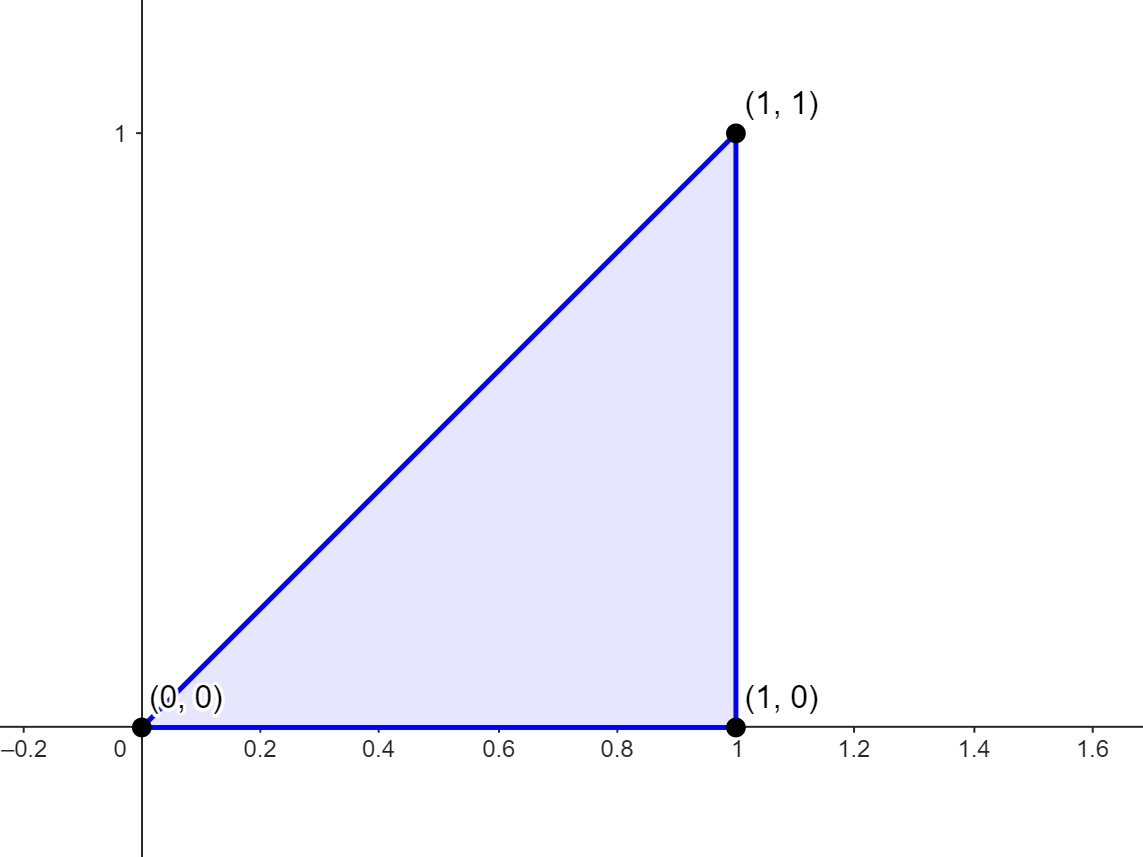
\includegraphics[width=\textwidth]{Capitoli/Capitolo4/Integrale 1.png}
    \end{minipage}
    \hfill
    \begin{minipage}{0.55\textwidth} 
    Tale insieme è un dominio normale sia rispetto all'asse $x$ che rispetto all'asse $y$. Si osservi che il risultato di tale integrale deve essere lo stesso in qualsiasi dei due casi.
    \end{minipage}
    \end{figure}
    Si consideri $D$ normale rispetto all'asse $x$, cioè:
    \begin{equation*}
        D= \left\{(x,y) \mid 0 \leq x \leq 1, 0 \leq y \leq x \right\}
    \end{equation*}
    Allora, applicando le formule di riduzione \eqref{Eq: Formula di riduzione integrali doppi 1}
    \begin{equation*}
    \begin{aligned}
        \iint\limits_D{xy}\,dx\,dy &= \int_{0}^{1}{\left(\int_{0}^{x}xy\,dy\right)}\,dx=  \int_{0}^{1}{x\left(\frac{y^2}{2}\Big|_{0}^{x}\right)\,dx = \int_{0}^{1}\frac{x^3}{2}\,dx} = \frac{1}{8}
    \end{aligned}
    \end{equation*}
    Considerando $D$ normale rispetto all'asse $y$
    \begin{equation*}
        D= \left\{(x,y) \mid 0 \leq y \leq 1, y \leq x \leq 1 \right\}
    \end{equation*}
    Allora applicando le formule di riduzione \eqref{Eq: Formula di riduzione integrali doppi 2}
    \begin{equation*}
        \iint\limits_D{xy}\,dx\,dy= \int_{0}^{1}{\left(\int_{y}^{1}{xy\,dx}\right)}\,dy = \int_{0}^{1}{y\left( \frac{x^2}{2}\Big|_{y}^1 \right)}\,dy= \frac{1}{2}\int_{0}^{1}{\left(y-y^3\right)}\,dy= \frac{1}{8}
    \end{equation*}
\end{example}
\begin{example}[TO-DO]
    Si consideri il seguente integrale doppio.
    \begin{equation*}
    \iint\limits_D e^\frac{x}{y}\, dx\,dy    
    \end{equation*}
    su $D=\left\{ (x,y) \mid \frac{1}{2} \leq x \leq 1, \sqrt[3]{x} \leq y \leq 1\right\}$
\end{example}
\subsubsection{Formula di cambiamento di variabili}
Così come si faceva per gli integrali in una dimensione, anche per gli integrali in due dimensioni è possibile effettuare cambi di variabile. Prima di mostrare come sia possibile, occorre fare delle precisazioni a quanto detto in precedenza.
\begin{definition} \label{Def: Dominio regolare}
    Si dice che $D$ è un \textbf{dominio normale regolare} se, presi $a,b \in \mathbb{R}$ e $f,g, \in C^1([a,b])$ tali che $f < g\ \forall x \in (a,b)$ è della forma
    \begin{equation}
        D= \left\{a \leq x \leq b, \ f(x) \leq y \leq g(x) \right\}
    \end{equation}
    Si può anche dire che $D \subset \mathbb{R}$ è normale regolare se è un'unione finita di domini normali regolari che non abbiano punti interni in comune.
    \end{definition}
    %\begin{oss}
    %\end{oss}
    \vspace*{6pt}
Per poter approfondire il discorso occorre capire cosa si intenda per funzione con derivata prima continua su un chiuso. Si supponga dunque $f: \Omega \to \mathbb{R}$ con $\Omega = \overline{\mathring{\Omega}}$ e $f \in C^0(\Omega)$. Se $x_0 \in \mathring{\Omega}$ è noto il significato di derivate parziali continue in $x_0$. Al contrario, se $x_0 \in \partial \Omega$, si definiscono, se esistono:
\begin{equation}
\begin{aligned}
    &\frac{\partial{f}}{\partial{x}}(x_0)= \lim_{\substack{x \to x_0 \\ x \in \mathring{\Omega}}} \frac{\partial f}{\partial x}(x)\\
    &\frac{\partial{f}}{\partial{y}}(x_0)= \lim_{\substack{x \to x_0 \\ x \in \mathring{\Omega}}} \frac{\partial f}{\partial y}(x)
\end{aligned}
\end{equation}
dove si suppone $f \in C^1(\mathring{\Omega})$.\\
È necessario svolgere tale precisazione perché per effettuare il cambio di variabili occorre definire una funzione a valori vettoriali che abbia come dominio l'insieme di integrazione nelle nuove variabili e come codominio quello nelle variabili originali. Pertanto, si consideri ora una funzione a valori vettoriali definita su due domini regolari, $D,\ D' \subseteq \mathbb{R}^2$ della forma:
\begin{equation}
\begin{aligned}
    \Phi: D' &\to D\\
    (u,v) &\mapsto \Phi(u,v)
\end{aligned}
\end{equation}
con $\Phi(u,v)=(\Phi_1(u,v), \Phi_2(u,v))$ e $\Phi \in C^1(D')$, con le derivate parziali prolungate in $\partial D'$ come sopra. Allora su di essa può essere definita la Jacobiana 
\begin{equation}
    J_f(u,v)=\begin{pmatrix}
        \frac{\partial \Phi_1}{\partial x}(u,v) & \frac{\partial \Phi_1}{\partial y} (u,v)\\
        \frac{\partial \Phi_2}{\partial x} (u,v) & \frac{\partial \Phi_2}{\partial y} (u,v)
    \end{pmatrix}
\end{equation}
Ciò detto, si è in possesso di tutti gli strumenti necessari per la formulazione del teorema di cambiamento di variabili.
\begin{theorem}[Formula di cambiamento di variabili] \label{Teo: Formula cambiamento variabili}
    Siano $D, D'$ domini regolari di $\mathbb{R}^2$ e $\Phi: D' \to D$ di classe $C^1$ biunivoca e tale che $\det(J_f(u,v)) \neq 0\ \forall(u,v) \in D'$. Allora, per ogni $f \in C^0(D)$ vale
    \begin{equation} \label{Eq: Formula cambiamento di variabili}
        \iint\limits_{\substack{D\\=\Phi(D')}}
        f(x,y)\,dx\,dy= \iint\limits_{\substack{D'\\=\Phi^{-1}(D)}}{f(\Phi_1(u,v), \Phi_2(u,v))\left|\det(J_\Phi(u,v))\right|}\,du\,dv
    \end{equation}
\end{theorem}
\begin{example}
    Si risolva il seguente integrale.
    \begin{equation*}
        \iint\limits_{D}{\frac{x^3y}{x^2+y^2}\,dx\,dy}
    \end{equation*}
    con $D$ porzione di corona circolare con $r_1=1$ e $r_2=2$ nel primo quadrante compresa tra $y=\tfrac{\sqrt{3}}{3}x$ e $y=\sqrt{3}x$
\begin{figure}[H]
    \begin{minipage}{0.3\textwidth}
   \centering
   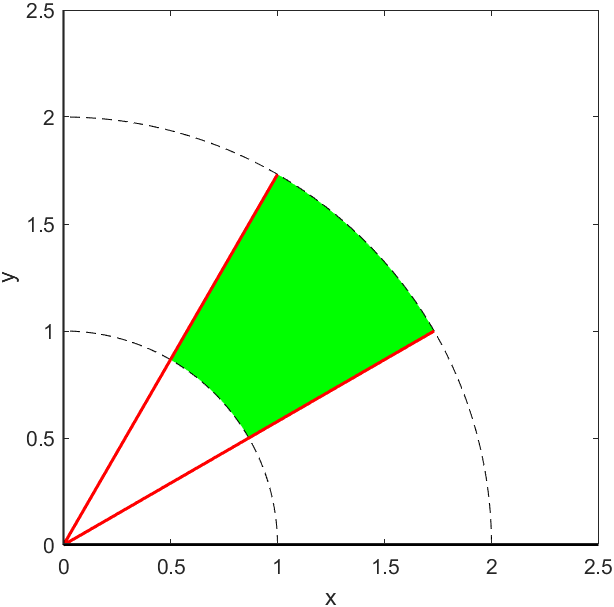
\includegraphics[width=\textwidth]{Capitoli/Capitolo4/Integrale 2.png}
    \end{minipage}
    \hfill
    \begin{minipage}{0.55\textwidth}
    In questo caso si può osservare come passando in coordinate polari sia estremamente più comodo risolvere tale integrale.\\
    Quindi
    \begin{equation*}
        \begin{cases}
            x= \varrho \cos \vartheta\\
            y= \varrho \sin \vartheta
        \end{cases}
    \end{equation*}
    Inoltre, lo Jacobiano è:
    \begin{equation*}
        \det\left(J_f(\varrho, \vartheta)\right)=\begin{vmatrix}
        \cos \vartheta & -\varrho \sin\vartheta\\
        \sin \vartheta & \varrho \cos\vartheta    
        \end{vmatrix}= \varrho
    \end{equation*}
    e $\arctan(\sqrt{3})= \tfrac{\pi}{3}$ e $\arctan(\tfrac{sqrt{3}}{3})=\tfrac{\pi}{6}$.
    \end{minipage}
\end{figure}
Pertanto, l'integrale diventa:
\begin{align*}
    &\iint\limits_{(\varrho, \vartheta) \in \Gamma=\left\{ 1 \leq \varrho \leq 2,\ \frac{\pi}{6} \leq \vartheta \frac{\pi}{3}\right\}}{\frac{\varrho^5 \cos^3 \vartheta \sin \vartheta}{\varrho^2}\,d\varrho\,d\vartheta}=\iint\limits_{\Gamma}{\varrho^3\left(\ \cos^3 \vartheta \sin \vartheta \right)\, d\varrho\,d\vartheta }=\\
    &=\int_{1}^{2}{\varrho^3\, d\varrho} \int_{\frac{\pi}{6}}^{\frac{\pi}{3}}{\cos^3\vartheta \sin \vartheta \, d\vartheta} = \left(\frac{\varrho^4}{4}\Big|_{1}^{2}\right)\left(\frac{\cos^4(\vartheta}{4}\Big|_{\frac{\pi}{6}}^\frac{\pi}{3}\right)= \frac{15}{32}
    \end{align*}
\end{example}
Si presti attenzione a quanto segue. Nel caso descritto sopra, l'angolo $\vartheta$ era definito su $\left[\tfrac{\pi}{6}, \tfrac{\pi}{3}\right]$ e dunque non presentava problemi.\\
Tuttavia, per quanto affermato nelle ipotesi del teorema \ref{Teo: Formula cambiamento variabili}, è necessario che $\Phi$ sia biunivoca affinché il cambiamento sia ammesso. Dunque, non è altrettanto garantito il cambiamento di variabili se $\vartheta \in [0, 2\pi]$, poiché $\Phi(\varrho, 0)=\Phi(\varrho, 2\pi)$ ovvero $\Phi$ non è biunivoca.
Tuttavia, per ovviare a tale problema, è possibile estendere il teorema menzionato prima nella forma che segue.
\begin{theorem}
    Sia $\Phi \in C^1(D')$ e siano $D'$ e $\Phi(D')=D$ unioni finite di domini normali. Esista poi una successione di domini regolari $D'_k \subseteq D'$ tale che $\Phi\big|_{D'_k}$ verifichi le ipotesi del teorema \ref{Teo: Formula cambiamento variabili}. Allora vale
    \begin{equation}
        m(D'_k) \to m(D') \qquad m(\Phi(D'_k)) \to m(\Phi(D'))
    \end{equation}
\end{theorem}
\vspace*{6pt}
\begin{oss}
    Si osservi che il passaggio a coordinate polari non è l'unico cambio di variabile degli integrali doppi.\\
    Generalmente, ogni qual volta vi sia la possibilità di semplificare $D$ rendendolo un dominio semplice rispetto ad una nuova variabile, è bene cambiare.\\ 
    Un esempio di nuove variabili può essere quello dato da un passaggio in \textit{coordinate ellittiche}
    \begin{equation}
        \begin{cases}
            x=\frac{\varrho}{a} \cos \vartheta\\
            y=\frac{\varrho}{b}\sin\vartheta
        \end{cases} \qquad a,b >0
    \end{equation}
\end{oss}
\section{Integrali tripli}
Si studino ora gli integrali tripli. Così come per gli integrali doppi, vale il discorso sulla costruzione mediante somme di Riemann. 
Si passi ora a descrivere le formule di riduzione.
\subsubsection{Formule di riduzione}
Siano $\mathcal{D}$ e $\mathcal{E}$ così definiti.
\begin{align}
    &\mathcal{D}=\left\{(x,y,z) \in \mathbb{R}^3 \mid (x,y) \in D \subseteq \mathbb{R}^2,\ \alpha(x, y) \leq \beta(x,y) \right\}\\
    &\mathcal{E}= \left\{(x,y,z) \in \mathbb{R}^3 \mid c_1\leq z \leq c_2, (x,y) \in D(z)\right\}
\end{align}
dove con $D$ si intende un dominio semplice. Siano poi $F \in C^0(\mathcal{D})$ e $G \in C^0(\mathcal{E}$.
Allora si dice che l'integrale è calcolato per \textit{fili paralleli} a $z$ se
\begin{equation}
    \iiint\limits_{\mathcal{D}} F(x,y,z)\, dx\, dy\,dz= \iint\limits_{D}{\left(\int_{\alpha(x,y)}^{\beta(x,y)}{F(x,y,z)\, dz}\right)}\,dx\, dy
\end{equation}
In alternativa, si dice che l'integrale è calcolato per \textit{strati paralleli} al piano $xy$ se
\begin{equation}
\iiint\limits_{\mathcal{E}}{G(x,y,z)\, dx\,dy\,dz} = \int_{c_1}^{c_2}{\left(\ \iint\limits_{D(z)}{G(x,y,z) \, dx\,dy} \right)\, dz}
\end{equation}
\begin{example}[TO-DO]
    Si calcoli il seguente integrale
    \begin{equation*}
    \iiint\limits_{\mathcal{D}}{x^3z}\,dx\,dy\,dz
    \end{equation*}
    su $\mathcal{D}= \left\{(x,y,z) \in \mathbb{R}^3 \mid z \geq 0,\ x^2+y^2+z^2\leq R^2\right\}$
\end{example}
\begin{oss}    
Si noti che integrare (in due o tre dimensioni) sulla costante $1$ equivale a calcolare la misura dell'insieme di integrazione ovvero, nel primo caso, calcolarne l'area, nel secondo, il volume.
\end{oss}
\subsubsection{Formule di cambiamento di variabili}
Anche nel caso di integrali in $R^3$ si può pensare di effettuare dei cambi di variabile. Il teorema delle formule di cambiamento delle variabili in $\mathbb{R}^3$ è pressoché analogo a quello in due dimensioni e raggiunge la seguente tesi:
\begin{equation}
    \iiint\limits_{\mathcal{D}}{f(x,y,z)}\,dx\,dy\,dz=\iiint_{\mathcal{D}'}{f(u,v,w)|\det(J_\Phi)|}\,du\,dv\,dw
\end{equation}
Si mostrino alcuni cambi di variabili notevoli.

Siano dette $\varphi \in [0, \pi]$ latitudine, $\vartheta \in [0, 2\pi]$ longitudine e sia $\varrho \in [0, R]$ con $R$ raggio della sfera, allora si dicono \textit{coordinate sferiche}
\begin{equation}
    \begin{cases}
    x=\varrho \sin \varphi \cos \vartheta\\
    y=\varrho \sin \varphi \sin \vartheta\\
    z=\varrho \cos \varphi
    \end{cases}
\end{equation}
ed il modulo del determinante della Jacobiana ottenuta da questo cambio di parametri vale $\varrho^2 \sin \varphi$.\\
Si parla invece di \textit{coordinate cilindriche} quando si applica
\begin{equation}
    \begin{cases}
        x=\varrho \cos \varphi\\
        y=\varrho \sin \varphi\\
        z=w
    \end{cases}
\end{equation}
ed il modulo del determinante della Jacobiana vale $\varrho$.
\subsubsection{Volume di solidi di rotazione}
Un'applicazione dell'integrale di volume è il calcolo dei volumi dei solidi di rotazione, ovvero quei solidi ottenuti dalla rotazione del grafico $G(f)$ di una funzione $f:[a,b] \to \mathbb{R}^+$ tale che $z \mapsto y$ attorno all'asse $z$ di un angolo di $2\pi$. Nello specifico vale il teorema di Pappo-Guldino.
\begin{theorem}[Teorema di Pappo-Guldino]
Sia $\Omega$ un solido di rotazione ottenuto come detto sopra. Allora
\begin{equation}
    \text{Vol}(\Omega)= \pi \int_a^b{f(z)^2}\, dz
\end{equation}
\end{theorem}
\begin{proof}
    Si rappresenti $\Omega$ per strati paralleli a $xy$. Ogni strato è un cerchio della forma $x^2+y^2 \leq f(z)^2$ con $z$ fissato, $a<z<b$ per costruzione.
    Quindi, 
    \begin{equation}
    \begin{aligned}
        \text{Vol}(\Omega)&= \iiint\limits_{\Omega}\,dx\,dy\,dz=\int_a^b{\left(\iint\limits_{\{x^2+y^2 \leq f(z)^2\}}{\,dx\,dy}\right)}\,dz=\\
        &= \int_{a}^{b}{\text{Area}(x^2+y^2 \leq f(z)^2)}\,dz = \pi\int_a^b{f(z)^2}\,dz
    \end{aligned}
    \end{equation}
\end{proof}
\section{Integrali impropri}
Anche in $\mathbb{R}^n$ è possibile definire gli \textbf{integrali impropri} (o generalizzati). In tal caso, occorre distinguere due possibili casi più un terzo che generalizza.
\paragraph{$\mathbf{\Omega \subseteq \mathbb{R}^n}$ illimitato; $\mathbf{f \in C^0(\Omega)}$ positiva}
Si può dire che $\Omega$ è misurabile se, per ogni plurirettangolo $P$ di $\mathbb{R}^n$ limitato, $\Omega \cap P$ è misurabile. Allora supponendo $\Omega$ tale, si consideri una successione crescente di $\Omega$ misurabili e limitati tale che 
\begin{equation}
 \Omega_j<\Omega_{j+1}\ \forall j \qquad \bigcup\limits_{j}{\Omega_j}=\Omega
\end{equation}
Allora, poiché $f$ è integrabile su $I_j=\int\limits_{\Omega_j}{f}$, si dice che $f$ è \textbf{integrabile in senso improprio} se esiste finito
\begin{equation}
    \lim_{j \to +\infty} I_j := \int\limits_\Omega{f}\,dx_1\, \dots \,dx_n
\end{equation}
\paragraph{$\mathbf{\Omega \subseteq \mathbb{R}^n}$ limitato; $\mathbf{f \in C^0(\Omega)}$ illimitata e positiva} Come prima, si può trattare $\Omega$ come unione di insiemi $\Omega_j$ misurabili in cui la funzione sia limitata. Allora, se esiste finito, si definisce \textbf{integrale improprio} di $f$
\begin{equation}
    \lim_{j \to +\infty} \int\limits_{\Omega_j}f :=    \int\limits_{\Omega} f\,dx_1\, \dots \,dx_n
\end{equation}
\paragraph{$\mathbf{f, \Omega}$ come prima ma $\mathbf{f}$ cambia segno} In tal caso si considerano le funzioni parte positiva e parte negativa definite come:
\begin{equation}
    f^+(x)=\max\{f(x), 0\} \qquad f^-(x)=\min\{-f(x), 0\}
\end{equation}
e, se $f^+,\ f^-$ sono integrabili impropriamente, si definisce l'integrale improprio di $f$ come:
\begin{equation*}
    \int\limits_{\Omega}f := \int\limits_{\Omega} f^+ - \int\limits_{\Omega} f^-
\end{equation*}
\subsubsection{Integrale della Gaussiana}
Si mostri infine un'applicazione dell'integrale improprio.
\begin{theorem}[Integrale della Gaussiana]
    \begin{equation}
    \int_{-\infty}^{+\infty}{e^{x^2}}\, dx = \sqrt{\pi}
    \end{equation}
\end{theorem}
\begin{proof}
    Si consideri innanzitutto il seguente integrale
    \begin{equation}
        I=\iint\limits_{\mathbb{R}^2}{e^{-(x^2+y^2)}}\,dx\,dy
    \end{equation}
    Per quanto detto, se tale integrale esiste allora può essere calcolato come
    \begin{equation} \label{Eq: Primo risultato teorema integrale gaussiana}
    \begin{aligned}
        I&=\lim_{R \to +\infty}{\iint_{B_R(0)}{e^{-(x^2+y^2)}}}\,dx\,dy \overset{\text{Polari}}{=} \lim_{R \to +\infty}{\iint\limits_{\substack{0 \leq \varrho \leq R^2\\ 0 \leq \vartheta \leq 2\pi}}{e^{-\varrho^2} \varrho}\,d\varrho\,d\vartheta}=\\
        &= 2\pi \lim_{R \to +\infty}{\frac{1}{2}}{e^{-\varrho^2}\Big|_{0}^{R}}= \pi \lim_{R \to +\infty}{(1-e^{-R^2})}= \pi
    \end{aligned}
    \end{equation}
    Tuttavia, la partizione tramite palle di raggio $R$ non è l'unica possibile. Si suddivida $\mathbb{R}^2$ in quadrati della forma
    \begin{equation}
        Q_j=(-J,J) \times (-J, J)
    \end{equation}
    Allora, 
    \begin{equation}
    \begin{aligned}
        I&= \lim_{J \to +\infty}{\iint\limits_{Q_J}{e^{-(x^2+y^2)}}\,dx\,dy}\overset{\eqref{Eq: Integrale doppio di funzioni separate}}{=} \lim_{J \to +\infty}{\int_{-J}^{+J}{e^{-x^2}}\, dx\ \int_{-J}^{+J}{e^{-y^2}}\,dy}=\\
        &=\lim_{J \to + \infty}\left(\int_{-J}^{+J}{ e^{-x^2}}\,dx\right)^2 = \left(\int_{-\infty}^{+\infty}{ e^{-x^2}}\,dx\right)^2 \overset{\eqref{Eq: Primo risultato teorema integrale gaussiana}}{=} \pi
    \end{aligned}
    \end{equation}
    Ne consegue che
    \begin{equation}
        \int_{-\infty}^{+\infty}{e^{x^2}}\, dx = \sqrt{\pi}
    \end{equation}
\end{proof}  \cleardoublepage
\chapter{Forme differenziali}
\section{Introduzione alle forme differenziali}
Si passi ora alla trattazione delle forme differenziali.
Per fare ciò, si consideri $A \subseteq \mathbb{R}^n$ aperto. Siano poi $a_1(x), \dots, a_n(x)$ con $x \in A$ funzioni continue in $A$ e siano $dx_1, \dots, dx_n$ funzioni lineari da $\R^n$ a $\R$ tali che $h \mapsto h_i$.
\begin{definition} \label{Def: Forma differenziale}
Si dice \textbf{forma differenziale} un'applicazione $\omega:\ x \in A \to  (\mathbb{R}^n)^*$, cioè il duale di $\mathbb{R}^n$, data dall'espressione:
\begin{equation}
    \omega= \omega(x)= \sum\limits_{i=1}^{n}{a_i(x)dx_i}
\end{equation}
con $a_i$ detti \textbf{coefficienti} della forma differenziale $\omega$.
\end{definition}
\begin{oss}
    Se $h$ è un vettore generico di $\R^n$, il valore assunto da $\omega(x)$ in $h$ è dato da:
    \begin{equation}
        \omega(x)(h)=\sum\limits_{i=1}^{n}{a_i(x)dx_i(h)}= \sum\limits_{i=1}^{n}{a_i(x)h_i}
    \end{equation}
\end{oss}
\begin{oss}
A tal proposito, si dice \textit{campo vettoriale} associato la funzione $F: A\subseteq \R^n \to \R^n$ data da
\begin{equation}
    F=F(x)=(a_1(x), \dots, a_n(x_n))
\end{equation}
Inoltre, si può notare che il legame tra i due è dato da:
\begin{equation} \label{Eq: Campo vettoriale}
    \omega(x)= \langle F(x), dx \rangle
\end{equation}
dove $dx= (dx_1,\dots, dx_n)$.
\end{oss}
\begin{oss}
Presa $f$ differenziabile in $A$, si può osservare che il suo differenziale $df$ sarà dato da
\begin{equation} \label{Eq: Differenziale}
    df(x)= \sum\limits_{i=1}^{n}{\frac{\partial f}{\partial x_i}(x)\ dx_i}= \langle \nabla f(x), dx\rangle
\end{equation}
\end{oss}
\section{Integrale curvilineo di seconda specie}
\begin{definition} \label{Def: Integrale curvilineo di seconda specie}
    Sia $A \subseteq \R$ e sia $\omega: A \to (\R)^*$ con coefficienti continui. Sia inoltre $\gamma$ una curva regolare di parametrizzazione $\varphi: [a, b] \to A$. Allora si definisce \textbf{integrale curvilineo di seconda specie} o integrale di $\omega$ lungo $\gamma$ la quantità:
    \begin{equation} \label{Eq: Integrale curvilineo di seconda specie}
        \int\limits_\gamma \omega := \int\limits_{a}^{b}\left( \sum\limits_{i=1}^{n}{a_i(\varphi(t))\ \varphi_i'(t)}\right)\, dt
    \end{equation}
\end{definition}
Per tale ragione, si può osservare che l'integrale curvilineo di seconda specie di un campo vettoriale $F$ associato ad una forma differenziale $\omega$ lungo una curva $\gamma$ è dato dall'integrale curvilineo di prima specie di 
\begin{equation}
    \int\limits_{\gamma}{\langle F, T \rangle}\, ds
\end{equation}
e in particolare vale:
\begin{equation}
    \int\limits_{\gamma}{\omega}= \int\limits_{a}^{b} {\langle F(\gamma(t)), \gamma'(t)\rangle}\, dt = \int\limits_{a}^{b} {\langle F(\gamma(t)), T(\gamma(t))\rangle} |\gamma'(t)|\, dt = \int\limits_{\gamma}{\langle F, T \rangle}\, ds
\end{equation}
Inoltre, vale il seguente risultato.
\begin{theorem}[Invarianza per equivalenza di curve] \label{Teo: Invarianza per equivalenza di curve dell'integrale curv di 2 specie}
    Siano $\gamma,\ , \gamma'$ due curve equivalenti e sia $\omega$ una forma differenziale definita in $A$. Allora
    \begin{equation}
        \int\limits_\gamma { \omega} = \int\limits_{\gamma'}{\omega}\quad \text{oppure} \quad \int\limits_\gamma { \omega} = -\int\limits_{\gamma'}{\omega}
    \end{equation}
    se sono percorse nello stesso verso o in verso opposto, rispettivamente.
\end{theorem}
\begin{proof}
    Per definizione di equivalenza di curve, prese 
    $\varphi: [a, b] \to \R^n$ parametrizzazione di $\gamma$ e $\psi:[c,d] \to \R^n$ parametrizzazione di $\gamma'$,  esiste un cambio di parametro ammissibile $\eta$ tale che $\varphi(t)= \psi(\eta(t))$ per ogni $t \in [a,b]$. Allora, 
    \begin{equation}
        \int\limits_\gamma {\omega}= \int\limits_{a}^{b}{\langle F(\varphi(t)), \varphi'(t) \rangle}\, dt = \int\limits_{a}^{b}{ \langle F(\psi(\eta(t))), \psi(\eta(t))\eta'(t)\rangle}\, dt
    \end{equation}
    dove $F$ è il campo vettoriale associato ad $\omega$.
    Perciò, mediante la sostituzione
    \begin{equation}
        \eta(t)=s \qquad \eta'(t)dt =ds
    \end{equation}
    si ha che, se le due curve sono percorse nello stesso verso, $\eta'(t) >0 $ e $\eta(a)=c,\ \eta(b)=d$ e
    \begin{equation}
    \int\limits_{\eta(a)=c}^{\eta(b)=d}{ \langle F(\psi(s)), \psi'(s)\rangle}\, ds \overset{\text{Costr.}}{=} \int\limits_{\gamma'}{\omega} 
    \end{equation}
    Altrimenti, se $\eta'(t) < 0 $,  $\eta(a)=d,\ \eta(b)=c$ e 
    \begin{equation}
     \int\limits_{\eta(a)=d}^{\eta(b)=c}{ \langle F(\psi(s)), \psi'(s)\rangle}\, ds = - \int\limits_{c}^{d}{\langle F(\psi(s)), \psi'(s)\rangle}\, ds\overset{\text{Costr.}}{=} -\int\limits_{\gamma'}{\omega} 
    \end{equation}
\end{proof}
\begin{oss}
    Per come è definito, si può notare che $\int\limits_{\gamma}{\omega}$ è il lavoro del campo vettoriale $F$ lungo $\gamma$.
\end{oss}
\section{Forme differenziali esatte}
In continuità con l'ultima osservazione, può essere approfondito il tema del lavoro di una forma differenziale lungo una certa curva $\gamma$. In particolare, scopo del paragrafo è stabilire sotto quali circostanze una forma differenziale possa dirsi \textit{esatta} e come tale gruppo possa essere caratterizzato.
\begin{definition} \label{Def: Forma differenziale esatta}
    Sia $\omega$ una forma differenziale su $A \subseteq \R^n$. Allora $\omega$ è detta \textbf{esatta} in $A$ se ammette primitiva $f$, cioè se essa è il differenziale di una certa $f \in C^1(A)$ tale che 
    \begin{equation}
        \omega = df
    \end{equation}
    In maniera equivalente, una forma differenziale esatta è una forma differenziale tale che
    \begin{equation} \label{Eq: Forma differenziale esatta}
        \exists\ \mathcal{U} \in C^1(A) \ \text{tale che}\ F=\nabla\mathcal{U}
    \end{equation}
\end{definition}
In termini fisici, così come prima si definiva campo vettoriale la funzione $F$ associata a $\omega$, ora, si definisce \textit{potenziale} $\U$ ciò che in analisi matematica è detto primitiva. Inoltre, sempre nell'ambito del lessico fisico, si può creare un ulteriore ponte sottolineando che una forma differenziale esatta è talvolta chiamata \textit{campo vettoriale conservativo}. Infatti, si può dimostrare che il lavoro di una forma differenziale esatta è dato dalla differenza di primitive valutate all'istante iniziale e a quello finale.
\begin{theorem} \label{Teo: Integrale di forme differenziali esatte}
    Sia $\omega$ una forma differenziale esatta e $\varphi: [a, b] \to \R^n$ una parametrizzazione della curva $\gamma$ regolare. Allora, detta $f$ primitiva di $\omega$, si ha che 
    \begin{equation}
        \int\limits_\gamma{\omega}= f(\varphi(b))-f(\varphi(a))
    \end{equation}
\end{theorem}
\begin{proof}
    Si risolva tale integrale.
    \begin{equation}
    \begin{aligned}
        \int\limits_{\gamma}{\omega} &\overset{\text{Def}}{=}\int\limits_{a}^{b}{\langle F(\varphi(t)), \varphi'(t)\rangle}\, dt \overset{\eqref{Eq: Forma differenziale esatta}}{=} \int\limits_{a}^{b}{\langle \nabla f(\varphi(t)), \varphi'(t) \rangle}\, dt =\\
        &\overset{\eqref{Eq: Derivata composta 1}}{=}\int\limits_{a}^{b}\frac{d}{dt}{f(\varphi(t))} \overset{\text{TFC}}{=} f(\varphi(b))- f(\varphi(a))
    \end{aligned}
    \end{equation}
\end{proof}
\paragraph{Giustificazione del termine \textit{conservativo}}
Si pensi ad $F$ come un campo di forze che agisce su una massa di $m=1$ e si consideri una generica traiettoria data da una curva $x=x(t)$ almeno di classe $C^2$ che soddisfi l'equazione differenziale 
\begin{equation}
    x''(t)=F(x(t)) \qquad \forall\ t \in \R
\end{equation}
Si introduca poi l'energia meccanica 
\begin{equation}
    E_m(t)= \frac{1}{2} |x'(t)|^2- f(x(t))
\end{equation}
con $f$ potenziale di $F$.\\
Allora, derivando tale relazione, si ha che
\begin{equation}
\begin{aligned}
        \frac{d}{dt}{E_m(t)}&=\frac{1}{2} \frac{d}{dt}{ \langle x'(t), x'(t) \rangle}- \frac{d}{dt}{f(x(t))}=\\
        &= \langle x''(t), x'(t) \rangle- \langle \nabla f(x(t)), x'(t) \rangle =\\
        &= \langle F(x(t)), x'(t) \rangle - \langle F(x(t)), x'(t) \rangle =0
\end{aligned}    
\end{equation}

Ciò significa che l'energia meccanica si \textit{conserva} lungo le traiettorie indotte dal campo $F$.
\begin{theorem}[Caratterizzazione delle forme esatte] \label{Teo: Caratterizzazione forme esatte}
Siano $A \subseteq \R^n$ aperto connesso, $\omega$ una forma differenziale in $A$ e $\gamma,\ \gamma_1,\ \gamma_2$ tre curve regolari a tratti con sostegno contenuto in $A$. Allora le seguenti affermazioni sono equivalenti:
\begin{enumerate}
    \item $\omega$ è esatta in A
    \item se $\gamma$ è chiusa allora 
    \begin{equation}
        \int\limits_{\gamma}{\omega}=0
    \end{equation}
    \item se $\gamma_1$, $\gamma_2$ hanno gli stessi estremi e lo stesso verso di percorrenza allora
    \begin{equation}
        \int\limits_{\gamma_1}{\omega} = \int\limits_{\gamma_2}{\omega}
    \end{equation}
\end{enumerate}
\end{theorem}
\begin{proof}
    Si dimostrino le tre affermazioni in questo ordine: $1 \Rightarrow 2 \Rightarrow 3 \Rightarrow 1$.\\
    $1 \Rightarrow 2$: Sia $\varphi: [a,b] \to A$ una parametrizzazione di $\gamma$. Poiché $\gamma$ è chiusa, si ha che $\varphi(a)=\varphi(b)$. Allora, siccome $\omega$ è esatta, vale 
    \begin{equation}
        \int\limits_{\gamma}{\omega} = f(\varphi(b))- f(\varphi(a)) = f(\varphi(a))-f(\varphi(a))=0
    \end{equation}
    $2 \Rightarrow 3$: Si considerino $\gamma_1,\ \gamma_2$ definite come nelle ipotesi di $(3)$. Siano poi:
    \begin{equation}
        \begin{aligned}
            &\varphi: [a,b] \to A \ \text{parametrizzazione di } \gamma_1\\
            &\psi:[c, d] \to A \ \text{parametrizzazione di } \gamma_2
        \end{aligned}
    \end{equation}
    Sia poi $\hat{\psi}$ la parametrizzazione che percorre $\psi$ in verso opposto, cioè
    \begin{equation}
        \hat{\psi}(t)= \psi(-t+b+d) \qquad t \in [b, b+d-c]
    \end{equation}
Si può verificare che: $\hat{\psi}(b)= \psi(d)$ e $\hat{\psi}(b+d-c)=\psi(c)$.\\
Allora, definita $\xi: [a, b+d-c] \to A$ come
\begin{equation}
    \xi(t)= \begin{cases}
        \varphi(t) \qquad & t \in [a,b]\\
        \hat{\psi}(t) \qquad & t \in [b, b+d-c]
    \end{cases}
\end{equation}
Si ha che per costruzione essa è regolare a tratti. Inoltre, si ha che:
\begin{equation}
\begin{aligned}
    &\xi(a)= \varphi(a)\\
    &\xi(b+d-c)= \hat(\psi(b+d-c))=\psi(c)=\varphi(a)
\end{aligned}
\end{equation}
cioè $\xi(t)$ è una curva chiusa. Allora, detta $\hat{\gamma}$ la curva di parametrizzazione $\xi(t)$, per il punto (2) si ha che:
\begin{equation}
\begin{aligned}
\int\limits_{\hat{{\gamma}}}{\omega} &= \int\limits_{a}^{b} \langle F(\varphi(t)), \varphi'(t)\rangle \, dt + \int\limits_{b}^{b+d-c}{\langle F(\hat{\psi}(t), \hat{\psi}(t) \rangle}\, dt=\\ 
&= \int\limits_{a}^{b} \langle F(\varphi(t)), \varphi'(t)\rangle \, dt - \int\limits_{c}^{d}{\langle F(\psi(t)), \psi'(t) \rangle}\, dt =\\
&= \int\limits_{\gamma_1}{\omega} - \int\limits_{\gamma_2}{\omega} = 0
\end{aligned}
\end{equation}
Da cui si ottiene la tesi.\\
$3 \Rightarrow 1$: Sia $x_0 \in A$ fissato. Dato $x \in A$, poiché $A$ è connesso per archi, esiste una curva $\gamma$ regolare a tratti che congiunga $x_0$ a $x$ con sostegno in A. Sia inoltre $\gamma$ percorsa da $x_0$ a $x$. Allora, si ponga
\begin{equation}
    f(x):=\int\limits_{\gamma}{\omega}
\end{equation}
In particolare si può osservare che grazie a (3) tale funzione è sempre ben definita e il suo valore non dipende dalla curva scelta.\\
L'obiettivo della dimostrazione è mostrare che $f \in C^1(A)$ e $df= \omega$.\\
Siano dunque $x=(x_1, \dots, x_n) \in A$, $h \in \R$ tali che $x+he_i \in A$. Sia poi $\varphi$ la curva di sostegno $[x, x+he_i]$, cioè
\begin{equation}
    \varphi= \begin{cases}
        x_1(t)=x_1\\
        \vdots\\
        x_i(t)=x_i+ht\\
        \vdots\\
        x_n(t)=x_n
    \end{cases}
    \qquad t \in [0,1]
\end{equation}
Sia poi $\gamma_1= \gamma \cup \varphi$, che, per costruzione, è regolare a tratti e congiunge $x_0$ a $x_0+he_i$. Tramite la definizione di $f$ si ottiene che
\begin{equation}
\begin{aligned}
    f(x_0+he_i)-f(x)&=\int\limits_{\gamma_1}{\omega}- \int\limits_{\gamma}{\omega}= \int\limits_{\gamma}{\omega}+\int\limits_{\varphi}{\omega}-\int\limits_{\gamma}{\omega}= \int\limits_{\varphi}{\omega}=\\
    &=\int\limits_{0}^{h}{\left[\sum\limits_{j=1}^{n}{a_j(\varphi(t))\varphi_j'(t)} \right] }\, dt=    \int\limits_{0}^{h}{a_i(\varphi(t))\cdot 1}\, dt =\\ 
    &=\int\limits_{0}^{h}{a_i(x_1, \dots, x_i+ht, \dots x_n)}\, dt
\end{aligned}
\end{equation}
Di conseguenza, 
\begin{equation}
\begin{aligned}
    \frac{\partial{f}}{\partial x_i}{(x)}&= \lim_{h\to 0}{\frac{f(x+he_i)-f(x)}{h}}= \frac{1}{h}{\int\limits_{0}^{h}{a_i(x_1, \dots, x_i+ht, \dots x_n)}\, dt}=\\
    &\overset{\text{TFC}}{=} a_i(x_1, \dots, x_i, \dots, x_n) = a_i (x)
\end{aligned}
\end{equation}
Reiterando per ogni $i$ si ottiene che $\nabla f(x)= (a_1(x), \dots, a_n(x))$, cioè $\omega$ è una forma esatta. 
\end{proof}
\section{Forme differenziali chiuse}
\begin{definition} \label{Def: Forma differenziale chiusa}
    Sia $\omega$ una forma differenziale definita in $A$ aperto di $\R^n$. Si dice che $\omega$ è \textbf{chiusa} in $A$ se
    \begin{equation}
        \frac{\partial a_i}{\partial x_j}(x)= \frac{\partial a_j}{\partial x_i} \qquad \forall\ x \in A,\ \forall\ i, j = 1, \dots, n
    \end{equation}
\end{definition}
Dal punto di vista fisico, dato un campo vettoriale $F=F(x)=(a_1(x), \dots, a_n(x))$ definito in $A \subseteq \R^n$, lo si dice \textit{campo vettoriale irrotazionale} se vale (\theequation). 
\begin{theorem} \label{Teo: Forma esatta => forma chiusa}
    Sia $\omega: A \subseteq \R^n \to (\R)^*$ una forma differenziale esatta di classe $C^1(A)$. Allora $\omega$ è chiusa in $A$.
\end{theorem}
\begin{proof}
    Poiché $\omega$ è esatta, per definizione, ne esiste una primitiva $f$ tale che
    \begin{equation}
        \omega= df \iff a_i(x)=\frac{\partial f }{\partial x_i}(x) \qquad \forall\ x \in A,\ \forall\ i=1, \dots, n
    \end{equation}
    Poiché poi $a_i \in C^1(A)$, si ha che $f$ deve essere di classe $C^2(A)$. Pertanto, dal teorema di Schwarz (\ref{Teo: Schwarz}) si ottiene
    \begin{equation}
        \frac{\partial a_i}{\partial x_j}(x)= \frac{\partial f}{\partial x_j \partial x_i}(x) = \frac{\partial f}{\partial x_i \partial x_j}(x) = \frac{\partial a_j}{\partial x_i}(x)= 
    \end{equation}
    cioè la tesi.
\end{proof}
In maniera analoga, si ha che un campo conservativo $F$ definito su un aperto $A$ di $\R^n$ di classe $C^1(A)$ è ivi irrotazionale.
\begin{example}
    Si può notare che in tale teorema non vale l'implicazione inversa. Infatti, presa la forma differenziale in $A=\R^2\setminus \left\{ (0,0)\right\} $ definita da
    \begin{equation*}
        \omega(x,y)= - \frac{y}{x^2+y^2}dx+ \frac{x}{x^2+y^2}dy
    \end{equation*}
    si può osservare che
    \begin{equation*}
        \begin{aligned}
            &a_1(x, y)= - \frac{y}{x^2+y^2}, \qquad &\frac{\partial a_1}{\partial y} (x, y) = \frac{y^2-x^2}{\left(x^2+y^2 \right)^2} \\
            &a_2(x,y)= \frac{x}{x^2+y^2} \qquad &\frac{\partial a_2}{\partial x} (x, y) = \frac{y^2-x^2}{\left(x^2+y^2 \right)^2}
        \end{aligned}
    \end{equation*}
    cioè che $\omega(x,y)$ è chiusa in $A$.\\
    Si consideri ora la curva chiusa $\gamma$ di sostegno
    \begin{equation*}
        \gamma= \begin{cases}
            x= \cos t\\
            y= \sin t
        \end{cases}
        \qquad t \in \left[\ 0, 2 \pi \right]
    \end{equation*}
    Si ha:
    \begin{equation*}
    \int\limits_{\gamma}{\omega}= \int\limits_{0}^{2\pi}{- \frac{\sin t}{1} (-\sin t) + \frac{\cos t}{1} (\cos t)}\, dt = \int\limits_{0}^{2\pi}{\,dt}= 2\pi \neq 0
    \end{equation*}
    Quindi, non vale il teorema \ref{Teo: Caratterizzazione forme esatte}. Pertanto $\omega$ è chiusa ma non esatta.
\end{example}
\begin{definition} \label{Def: Rotore}
Dato un campo $F= F(x,y,z)= (a_1(x,y,z), a_2(x,y,z), a_3(x,y,z)$ definito in $A \subseteq \R^3$, si definisce \textbf{rotore} ($\Rot(F)$) l'operatore di $\R^3$ dato da
\begin{equation}
\nabla \wedge F = \left| \begin{matrix}
    i & j & k \\
    \partial x & \partial y & \partial z\\
    a_1 & a_2 & a_3
\end{matrix}
\right|
= \left( \frac{\partial a_3}{\partial y} - \frac{\partial a_2}{\partial z} \right)i - \left( \frac{\partial a_3}{\partial x} - \frac{\partial a_1}{\partial z} \right)j + \left( \frac{\partial a_2}{\partial x} - \frac{\partial a_1}{\partial y}\right)k 
\end{equation}
\end{definition}
\begin{definition} \label{Def: Campo irrotazionale}
    Sia $\omega$ una forma differenziale cui sia associato un campo $F$. Allora, $F$ si dice irrotazionale se e solo se $\omega$ è chiusa e se e solo se
    \begin{equation}
      \Rot(F) = \nabla \wedge F = 0  
    \end{equation}
\end{definition}
\begin{definition} \label{Def: Divergenza}
    Dato un campo $F= F(x,y,z)= (a_1(x,y,z), a_2(x,y,z), a_3(x,y,z)$ definito in $A \subseteq \R^3$, si definisce \textbf{divergenza} di $F$ ($\Div(F)$) l'operatore di $\R^3$ dato da
    \begin{equation}
        \langle \nabla, F \rangle = \frac{\partial a_1}{\partial x} + \frac{\partial a_2}{\partial y} + \frac{\partial a_3}{\partial z}
    \end{equation}
\end{definition}
L'obiettivo di quanto segue è trovare una condizione sufficiente che leghi forme chiuse e forme esatte. 
\begin{definition}
    Sia $A \subseteq \R^n$ aperto connesso. Si dice che $A$ è \textbf{semplicemente connesso} se ogni curva $\gamma:[a,b] \to A$ chiusa, regolare a tratti e semplice, con sostegno interamente contenuto in $A$ può essere contratta con continuità ad un punto $x_0 \in A$.
\end{definition}
\begin{oss}
    La deformazione con continuità è nota in topologia come \textit{omotopia}.
\end{oss}
\begin{oss}
    Un generico $A$ aperto convesso o stellato è semplicemente connesso.
\end{oss}
\begin{example}
    Banalmente, $\R^n$ è semplicemente connesso.\\
    Scendendo più nel dettaglio, si può osservare che $\R^2 \setminus \left\{(x_0,y_0)\right\}$ non lo è.
    Inoltre, $\R^3 \setminus \left\{(x_0, y_0, z_0)\right\}$ è semplicemente connesso. Al contrario $\R^3 \setminus \left\{\text{retta}\right\}$ non lo è.\\
    In generale, $\R^n$ privato di un elemento di dimensione $n-1$ non è semplicemente connesso. Nei casi di dimensione inferiore sì.
\end{example}
\begin{theorem} \label{Teo: Forma chiusa => forma esatta in spazi semplicemente connessi}
    Sia $A$ aperto semplicemente connesso di $\R^n$. Sia poi $\omega: A \to (\R^n)^*$ una forma differenziale chiusa di classe $C^1(A)$. Allora $\omega$ è esatta.
\end{theorem}
\begin{oss}
    Si può osservare che tale teorema offre una condizione sufficiente per identificare le forme esatte.
\end{oss}
\begin{oss}
    Se è vero che, presa $f$ primitiva di $\omega$, $f+k$ con $k \in \R$ è ancora una primitiva di $\omega$, non è altrettanto vero che tutte le primitive di $\omega$ differiscano per una costante reale. Solitamente ciò accade in $A$ semplicemente connessi.
\end{oss}
\begin{example}
    Si mostri ora come sia possibile procedere per riconoscere le forme esatte.
\begin{enumerate}
    \item Controllare se $\omega$ sia chiusa. In caso negativo, decade la condizione necessaria (\ref{Teo: Forma esatta => forma chiusa}) e $\omega$ non è esatta. Altrimenti bisogna continuare nell'indagine.
    \item Controllare se $A$ sia semplicemente connesso. In caso affermativo, essa è anche esatta (\ref{Teo: Forma chiusa => forma esatta in spazi semplicemente connessi}). Altrimenti bisogna andare avanti e tentare due strade:
    \begin{itemize}
        \item Cercare un'eventuale primitiva $f$ tale che $\omega= df$. Se essa esiste, $\omega$ è esatta per definizione.
        \item Cercare una curva $\gamma$ tale che $\int_{\gamma}{\omega} \neq 0$. Se essa esiste, $\omega$ non è esatta (\ref{Teo: Caratterizzazione forme esatte}). 
    \end{itemize}
\end{enumerate}
\end{example}
\section{Formule di Gauss-Green}
Prima di affrontare le formule di Gauss-Green e le conseguenze che ne discendono, occorre fare prima un accenno su cosa si intenda per orientazione della frontiera di un dominio.
\paragraph{Dominio normale}
In un \textit{dominio normale} (\ref{Def: Dominio normale}) $D$ come un generico
 \begin{equation}
 D=\left\{ (x,y) \in \R^2 \mid a<x<b,\ \alpha(x)<y<\beta(x)\right\}
 \end{equation}
 si dice che la sua frontiera è positivamente orientata se è percorsa in senso antiorario e lo si indica con $\ppartial D$.
 \paragraph{Dominio regolare}
 In un \textit{dominio regolare} (\ref{Def: Dominio regolare}) $D$, si ha che la sua frontiera $\partial D$ è unione di un numero finito di curve regolari a tratti, pertanto, a meno di un numero finito di punti, è ben definito il versore tangente $T$. Si definisce allora $N$ il versore normale esterno a $D$ laddove $T$ sia ben definito e si dice che la frontiera di $D$ è orientata positivamente se $\left\{N,T\right\}$ è equiversa a $\left\{i, j\right\}$ e lo si indica con $\ppartial D$.
 Si mostri ora un esempio di frontiera positivamente orientata.
 \begin{figure}[H]
     \centering
     \begin{minipage}{0.5\textwidth}
     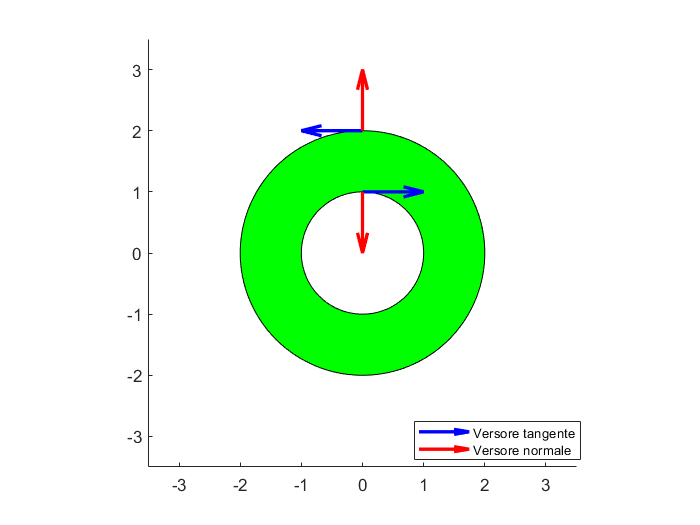
\includegraphics[width=\textwidth]{Capitoli/Capitolo5/Bordo orientato.png}
     \end{minipage}
     \begin{minipage}{0.4\textwidth}
         Affinché la frontiera della corona circolare sia orientata positivamente, occorre che la coppia di versori $N,\ T$ sia disposta come in figura. Da ciò si osserva che la circonferenza esterna deve essere percorsa in senso antiorario, quella interna nel senso opposto.
     \end{minipage}
 \end{figure}
 \begin{theorem}[Formule di Gauss-Green per domini regolari] \label{Teo: Formule di Gauss Green}
 Sia $f: D\subseteq \R^2 \to \R$ di classe $C^1(D)$. Se $D$ è un dominio normale regolare rispetto a $x$ si ha che
 \begin{equation} \label{Eq: Gauss-Green per dimostrazione}
     \iint\limits_D{\frac{\partial f}{\partial y}(x,y)}\,dx\,dy= -\int\limits_{\ppartial D}{f(x,y)}\,dx
 \end{equation}
     Se invece $D$ è un dominio normale regolare rispetto a $y$, vale
     \begin{equation}
    \iint\limits_D{\frac{\partial f}{\partial x}(x,y)}\,dx\,dy= \int\limits_{\ppartial D}{f(x,y)}\,dy
     \end{equation}
 \end{theorem}
 \begin{proof}
 Sia $D$ definito come segue:
        \begin{equation}
          D=  \left\{ (x,y) \in \R^2 \mid a \leq x \leq b,\ \alpha(x) \leq y \leq \beta(x)\right\}
        \end{equation}
Allora si ha che la frontiera di tale insieme può essere rappresentata come l'unione dei sostegni di quattro curve, come in figura.
 \begin{figure}[H]
     \centering
     \begin{minipage}{0.3\textwidth}
     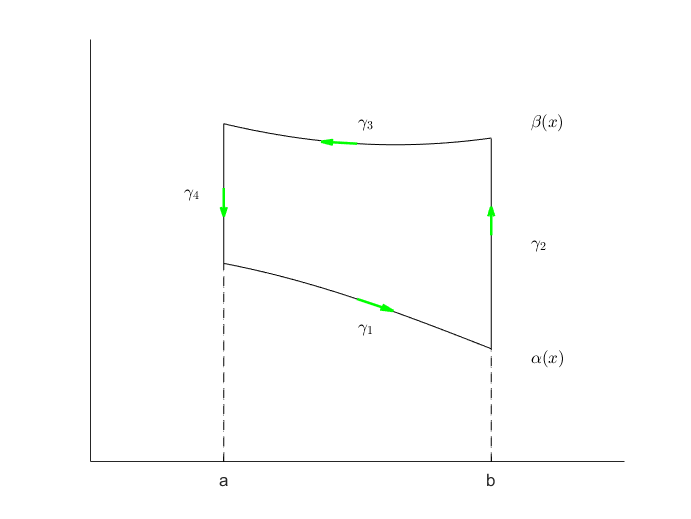
\includegraphics[width=\textwidth]{Capitoli/Capitolo5/Curve per GG.png}
     \end{minipage}
     \begin{minipage}{0.63\textwidth}
        Si parametrizzino i vari tratti di curva: 
        \begin{equation}
            \begin{aligned}
                &\gamma_1:\ \varphi_1(t)= \begin{cases}
                    t\\
                    \alpha(t)
                \end{cases}
                \quad t \in [a,b]\\
                &\gamma_2:\ \varphi_2(t)= \begin{cases}
                    b\\
                    t
                \end{cases}
                \quad t \in [\alpha(b), \beta(b)]\\
                &\gamma_3:\ \varphi_3(t)= \begin{cases}
                    a+b-t\\
                    \beta(a+b-t)
                \end{cases}
                \quad t \in [a,b]\\
                &\gamma_4: \varphi_4(t)= \begin{cases}
                    a\\
                    \beta(a)+\alpha(a)-t
                \end{cases}
                \quad t \in [\alpha(a), \beta(a)]
            \end{aligned}
        \end{equation}
     \end{minipage}
 \end{figure}
 \flushleft Dunque, si mostri, senza perdita di generalità, l'equivalenza degli integrali nella \eqref{Eq: Gauss-Green per dimostrazione}.
 \begin{equation}
    \begin{aligned}
     \iint\limits_D{\frac{\partial f}{\partial y}(x,y)}\,dx\,dy &\overset{\eqref{Eq: Formula di riduzione integrali doppi 1}}{=} \int\limits_{a}^{b}{\left( \int\limits_{\alpha(x)}^{\beta(x)}\frac{\partial f}{\partial y}(x,y)\,dy \right)}\, dx \overset{\text{TFC}}{=}\int\limits_{a}^{b}{ f(x, \beta(x))- f(x, \alpha(x))}\, dx
     \end{aligned}
 \end{equation}
Inoltre, 
\begin{equation}
\begin{aligned}
    \int\limits_{\ppartial D}{f}\, dx &= \sum\limits_{i=1}^{4} \int\limits_{\gamma_i}{f}\,dx =
    \int\limits_{a}^{b}{f(t, \alpha(t)) t'}\, dt+ \int\limits_{\alpha(b)}^{\beta(b)}{f(b,t)b'}\, dt +\\
    &+\int\limits_{a}^{b}{f(a+b-t, \beta(a+b-t))(a+b-t)'}\, dt + \int\limits_{\alpha(a)}^{\beta(a)}{f(a, \beta(a)+\alpha(a)-t) a'}\, dt=\\
    &= \int\limits_{a}^{b}{f(t, \alpha(t))}\, dt + \int\limits_{a}^{b}{-f(a+b-t, \beta(a+b-t))}\, dt =\\
    &\overset{\substack{\text{Nel }\#2:\\ a+b-t=s\\ -dt=ds}}{=} \int\limits_a^b{f(t, \alpha(t))}\, dt + \int\limits_a^b{f(s, \beta(s))}\, ds = \int\limits_{a}^{b}{f(t, \alpha(t))- f(t, \beta(t))}\, dt=\\
    &=-\int\limits_{a}^{b}{ f(t, \beta(t))- f(t, \alpha(t))}\, dt
    \end{aligned}
\end{equation}
Cioè la tesi.\\
Il ragionamento e la dimostrazione per la seconda parte della tesi sono analoghi.
 \end{proof}
 Dal teorema discende come corollario quanto segue.
 \begin{corollary}
     Sia $D$ un dominio normale regolare rispetto a entrambi gli assi e sia $\omega= P(x,y)dx+ Q(x,y)dy$ una forma differenziale di classe $C^1(D)$. Allora
     \begin{equation}
         \iint\limits_{D}{\left[\frac{\partial Q}{\partial x} (x,y)- \frac{\partial P}{\partial y}(x,y)\right]}\, dx\, dy = \int\limits_{\ppartial D} \omega
     \end{equation}
\end{corollary}
\begin{proof}
    La dimostrazione discende dall'applicazione del teorema precedente. Infatti,
    \begin{equation}
        \begin{aligned}
            &\iint\limits_{D}{\frac{\partial Q}{\partial x} (x,y)}\,dx\,dy =  \int\limits_{\ppartial D}{Q(x,y)}\,dy\\
            &\iint\limits_{D}{\frac{\partial P}{\partial y} (x,y)}\,dx\,dy =  -\int\limits_{\ppartial D}{P(x,y)}\,dx
        \end{aligned}
    \end{equation}
    Perciò, unendo tali risultati si ha che
    \begin{equation}
      \iint\limits_{D}{\left[\frac{\partial Q}{\partial x} (x,y)- \frac{\partial P}{\partial y}(x,y)\right]}\, dx\, dy = \int\limits_{\ppartial D}{Q(x,y)}\,dy - \left(  -\int\limits_{\ppartial D}{P(x,y)}\,dx\right)= \int\limits_{\ppartial D} \omega  
    \end{equation}
\end{proof}
\begin{oss}
A questo punto si può inoltre aggiungere che se $D$ è un dominio regolare qualsiasi definito come 
\begin{equation}
    D = \bigcup_{j=1}^{N} D_j
\end{equation}
allora continuano a valere le formule di Gauss-Green. Una dimostrazione di tale fatto si può avere sommando per additività gli integrali calcolati sui singoli tratti di frontiera. Infatti, laddove $\ppartial D_i$ e $\ppartial D_j$ coincidono, si ha che i versori normali hanno verso opposto e il loro contributo è nullo, lasciando come integrale risultante proprio
\begin{equation}
    \int\limits_{\ppartial D}{\omega}
\end{equation}
\end{oss}
Le formule di Gauss-Green possono essere utilizzate per il calcolo di aree racchiuse da curve. Infatti vale il seguente corollario.
\begin{corollary}[Gauss-Green per il calcolo di aree racchiuse da una curva]
Sia $D \subseteq \R^2$ un dominio regolare. Allora,
\begin{equation}
    \area(D)= \int\limits_{\ppartial D}{x}\, dy = -\int\limits_{\ppartial D}{y}\, dx = \frac{1}{\alpha+\beta}{\int\limits_{\ppartial D}{\alpha x dy - \beta y dx}} \qquad \forall\ \alpha, \beta \in \R,\ \alpha+\beta \neq 0
\end{equation}
\end{corollary}
\begin{proof}
    Per definizione 
    \begin{equation}
        \area(D)= \iint\limits_{D}{1}\,dx\, dy
    \end{equation}
    Allora si ha che
    \begin{align}
        &1= \frac{\partial f}{\partial y} \Rightarrow f(x,y)= y \Rightarrow \area(D)= \iint\limits_{D} \frac{\partial f}{\partial y} \overset{\text{G.G.}}{=}  -\int\limits_{\ppartial D}{y}\,dx\\
      &  1=\frac{\partial f}{\partial x} \Rightarrow f(x,y)= x \Rightarrow \area(D)= \iint\limits_{D} \frac{\partial f}{\partial x} \overset{\text{G.G.}}{=}  \int\limits_{\ppartial D}{x}\,dy
    \end{align}
    Perciò, si ha che
    \begin{equation}
        (\alpha+\beta)\area(D)= \int\limits_{\ppartial D}{\alpha x dy - \beta y dx} \Rightarrow \area(D)=  \frac{1}{\alpha+\beta}{\int\limits_{\ppartial D}{\alpha x dy - \beta y dx}}
    \end{equation}
\end{proof}\cleardoublepage
\chapter{Superfici}
D'ora in avanti nel corso del capitolo sia $D \subseteq \R^2$ un dominio connesso tale che il suo interno $\mathring{D}=A$ con $A$ aperto.
\begin{definition} \label{Def: Superficie parametrica}
    Una \textbf{superficie parametrica} in $\R^3$ è un'applicazione continua $r: D \to \R^3$
    \begin{equation}
        r(u,v)=(x(u,v), y(u,v), z(u,v))
    \end{equation}
\end{definition}
Una superficie parametrica è anche descritta tramite le proprie \textit{equazioni parametriche}
\begin{equation}
    r: \begin{cases}
        x=x(u,v)\\
        y=y(u,v)\\
        z=z(u,v)
    \end{cases}
    \qquad (u,v) \in D
\end{equation}
\begin{definition} \label{Def: Sostegno di una superficie}
    Si dice \textbf{sostegno di una superficie} l'insieme $S=r(D)$
\end{definition}
In realtà una superficie propriamente detta è la coppia data da una sua parametrizzazione e il suo sostegno.\\
Inoltre, come per le curve, è possibile parlare di riparametrizzazioni di una superficie. Tuttavia, tale discorso non verrà approfondito.
\begin{definition} \label{Def: Superficie di classe C^k}
    Una superficie $r$ è detta di classe $\mathbf{C^K}$ se $r \in C^k(D)$.
\end{definition}
\begin{definition} \label{Def: Superficie semplice}
    Una superficie $r$ si dice \textbf{semplice} se $r|_A$ è iniettiva e $r(A) \cap\ r(D)= \emptyset$
\end{definition}
\begin{definition} \label{Def: Superficie regolare}
    Una superficie $r: D \to \R^3$ è detta \textbf{regolare} se essa è una superficie semplice di classe $C^1(D)$ tale che
    \begin{equation}
        J_r(u,v)= \begin{pmatrix}
            \frac{\partial x}{\partial u}(u,v) & \frac{\partial x}{\partial v}(u,v)\\
            \frac{\partial y}{\partial u}(u,v) & \frac{\partial y}{\partial v}(u,v)\\
            \frac{\partial z}{\partial u}(u,v) & \frac{\partial z}{\partial v}(u,v)
        \end{pmatrix}
    \end{equation}
abbia rango 2 per ogni $(u,v) \in \mathring{D}$
\end{definition}
\begin{definition}
    Sia $(\overline{u}, \overline{v}) \in D$ tale che $\rank(J_r(\overline{u}, \overline{v}))< 2$, allora esso è detto \textbf{punto singolare}
\end{definition}
Si può pertanto notare che la nozione di regolarità garantisce che $\tfrac{\partial r}{\partial u} (u,v)$ e $\tfrac{\partial r}{\partial v} (u,v)$ siano linearmente indipendenti per ogni $(u,v) \in \mathring{D}$. Ciò ha come conseguenza che sia ben definito il piano tangente a $S=r(D)$ in $r(u,v)$.
\begin{definition} \label{Def: Piano tangente ad una superficie}
    Sia $S$ una superficie regolare avente una parametrizzazione $r: D \to \R^3$ e sia $(u_0,v_0) \in \mathring{D}$. Allora si dice \textbf{piano tangente} a $(u_0, v_0)$ il piano definito da 
    \begin{equation}
        \Span\left\{\frac{\partial r}{\partial u} (u_0,v_0), \frac{\partial r}{\partial v} (u_0,v_0)\right\}
    \end{equation}
\end{definition}
Rispetto a tale fatto si può dire di più. Si prenda una curva regolare $\gamma$ contenuta in $D$. Si può verificare che $r$ trasforma $\gamma$ in una curva regolare $\Tilde{\gamma}:[a,b] \to S \subseteq \R^3$ di equazioni parametriche
\begin{equation}
\Tilde{\gamma}(t)= \begin{cases} 
x= x(\gamma_1(t), \gamma_2(t))\\ 
y= y(\gamma_1(t), \gamma_2(t))\\
z= z(\gamma_1(t), \gamma_2(t))
\end{cases}
\qquad t \in [a,b]
\end{equation}
Poiché $\gamma$ è regolare, anche $\Tilde{\gamma}$ è di classe $C^1$ su $[a,b]$ e in particolare
\begin{equation}
    \Tilde{\gamma}'(t)\overset{\ref{Teo: Derivata composta di f. vettoriali}}{=}
        \begin{pmatrix}
            \frac{\partial x}{\partial u}(\gamma_1,\gamma_2) & \frac{\partial x}{\partial v}(\gamma_1,\gamma_2)\\
            \frac{\partial y}{\partial u}(\gamma_1,\gamma_2) & \frac{\partial y}{\partial v}(\gamma_1,\gamma_2)\\
            \frac{\partial z}{\partial u}(\gamma_1,\gamma_2) & \frac{\partial z}{\partial v}(\gamma_1,\gamma_2)
        \end{pmatrix}
        (\gamma_1', \gamma_2') = \frac{\partial r}{\partial u}(\gamma(t))\gamma_1'(t) + \frac{\partial r}{\partial v}(\gamma(t))\gamma_2'(t)
\end{equation}
si può dedurre che per ogni $t \in [a,b]$ $\Tilde{\gamma}'$ è combinazione lineare dei generatori linearmente indipendenti del piano tangente. Ciò significa che il piano tangente contiene tutte le tangenti in $r(u,v)$ a curve regolari con sostegno in $S$ passanti per $r(u,v)$.
\begin{definition} \label{Def: Versore normale a una superficie}
    Sia $S$ una superficie regolare in ogni punto $(u,v)\in \mathring{D}$ di parametrizzazione $r$. Allora su $S$ è ben definito il \textbf{versore normale} a $S$ in $P=(u_0,v_0) \in \mathring{D}$ ed è dato da
    \begin{equation}
        \nu(P)= \pm \frac{\frac{\partial r}{\partial u} \wedge \frac{\partial r}{\partial v}}{\left|\frac{\partial r}{\partial u} \wedge \frac{\partial r}{\partial v}\right|}
    \end{equation}
\end{definition}
    In aggiunta, poiché il piano tangente è per definizione ortogonale a $\nu(P)=(\nu_1(P), \nu_2(P), \nu_3(P))$, la sua equazione è:
    \begin{equation} \label{Eq: Equazione piano tangente a una superficie}
        \nu_1(P)(x-x(u,v))+ \nu_2(P)(y-y(u,v))+\nu_3(P)(z-z(u,v))=0
    \end{equation}
\section{Superfici orientabili}
Sia $r: D=\overline{A} \to \R^3$ una superficie regolare. Allora si dice $S_0:= r(A)$ \textbf{parte interna} di $S$. Inoltre, per regolarità di $S$ è ben definita e continua rispetto a $(x,y,z)$ la funzione
\begin{equation}
    \nu: P \in S_0 \subseteq \R^3 \mapsto \nu(P) \in \R^3
\end{equation}
\begin{oss}
    La continuità di $\nu$ discende dal teorema di invertibilità globale, di cui però non si è parlato durante il corso.
\end{oss}
\begin{definition} \label{Def: Superficie orientabile}
Una superficie $S$ si dice \textbf{orientabile} se $\nu$ può essere estesa con continuità da $S_0$ a $S$. In maniera equivalente, $S$ si dice orientabile se per ogni curva chiusa continua $\varphi: [a,b] \to S$ si ha che
\begin{equation}
    \lim_{t \to b^-}{\nu(\varphi(t))}=\nu(\varphi(a))
\end{equation}
\end{definition}
\begin{example} [Nastro di Möbius]
    Si mostri un esempio di superficie non orientabile.
\begin{figure}[H]
     \centering
     \begin{minipage}{0.4\textwidth}
     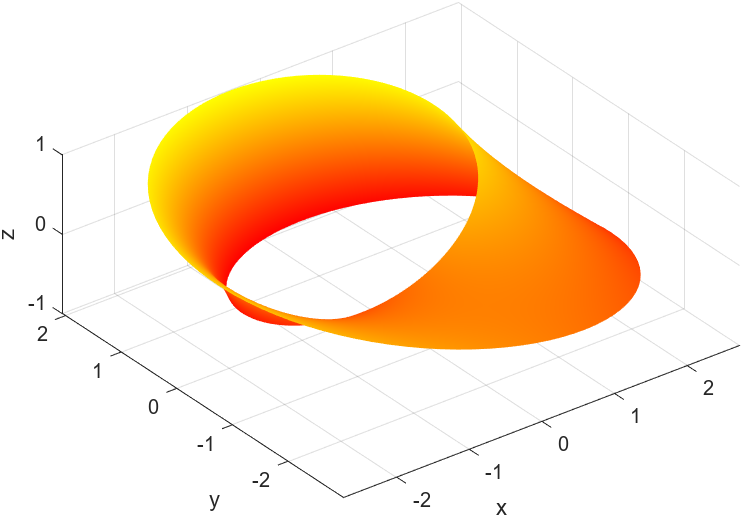
\includegraphics[width=\textwidth]{Capitoli/Capitolo6/Nastro di Moebius.png}
     \end{minipage}
     \begin{minipage}{0.55\textwidth}
        Una possibile parametrizzazione di tale superficie può essere
        \begin{equation*}
            r(u,v)= \begin{cases}
                \left(2-v \sin\left(\frac{u}{2}\right)\right) \sin(u)\\
                \left(2-v \sin\left(\frac{u}{2}\right)\right) \cos (u)\\
                v \cos\left(\frac{u}{2}\right)
            \end{cases}
        \end{equation*}
    con $u \in [0, 2\pi], v \in [-1,1]$
     \end{minipage}
 \end{figure}
 \begin{figure}[H]
     \centering
     \begin{minipage}{0.5\textwidth}
 In particolare, studiando i punti in cui $v$ sia nullo si ha che
 \begin{align*}
     & n=\frac{\partial r}{\partial u} \wedge \frac{\partial r}{\partial v}=(2\sin u, 2 \cos u, 0)\\
     &\lim_{u \to 0^+} n (u,0) = (0,-2,0)\\
     &\lim_{u \to 2\pi^-} n (u,0) = (0,2,0)
 \end{align*}
 e ciò non rispetta la definizione di superficie orientabile.
 \end{minipage}
 \begin{minipage}{0.3\textwidth}
     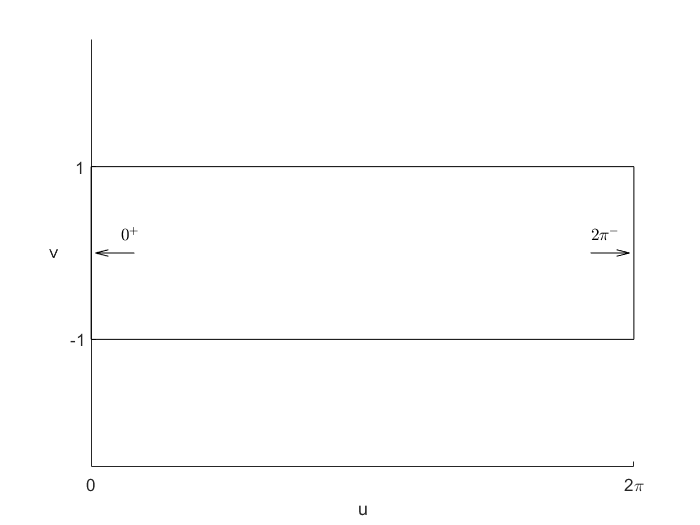
\includegraphics[width=\textwidth]{Capitoli/Capitolo6/Area per calcolo orientazione.png}
 \end{minipage}
 \end{figure}
 \end{example}
 \begin{example}
     Diversamente dal nastro di Möbius, si può osservare che i grafici di funzioni in due variabili $z=f(x,y)$ di classe $C^1$ sono superfici orientabili il cui sostegno è dato dal grafico $\mathcal{G}(f)$.
     Le equazioni parametriche della superficie sono:
     \begin{equation*}
         r(u,v)=\begin{cases}
             x= u\\
             y=v\\
             z=f(u,v)
         \end{cases}
     \end{equation*}
     Calcolando le derivate parziali ed il loro prodotto vettoriale si ha che
     \begin{equation*}
        \begin{aligned}
            &\frac{\partial r}{\partial u} = \left( 1, 0, \frac{\partial f}{\partial u}(u,v)\right)\\
            &\frac{\partial r}{\partial v} = \left( 0, 1, \frac{\partial f}{\partial v}(u,v)\right)\\
        \end{aligned}
            \qquad \Rightarrow \quad \nu(u,v)= \frac{\left(-\frac{\partial f}{\partial u}(u,v), -\frac{\partial f}{\partial v}(u,v), 1\right)}{\sqrt{1+ \left| \nabla f(u,v) \right|^2}}
     \end{equation*}
     Vale la pena notare che invertendo le variabili (ad esempio $x=v,\ y=u$) si ha un cambio di orientazione. Di conseguenza, l'orientazione dipende dalla parametrizzazione scelta.\\
     Inoltre, tramite il normale, è possibile distinguere tra "sopra" e  "sotto" o tra "dentro" e "fuori".
     \begin{figure}[H]
         \centering
         \begin{minipage}{0.4\textwidth}
         Si prenda ad esempio un paraboloide di equazione:
         \begin{align*}
             r(u,v)= \begin{cases}
                 x=u\\
                 y=v\\
                 z=u^2+v^2
             \end{cases}
         \end{align*}
        con $u \in [-1.5, +1.5],\ v \in [-1.5, +1.5]$.\\
        Calcolando, secondo le diverse convenzioni di segno, il versore normale è possibile visualizzare graficamente quanto asserito prima rispetto al "sopra" e "sotto".
     \end{minipage}
    \begin{minipage}{0.5\textwidth}
        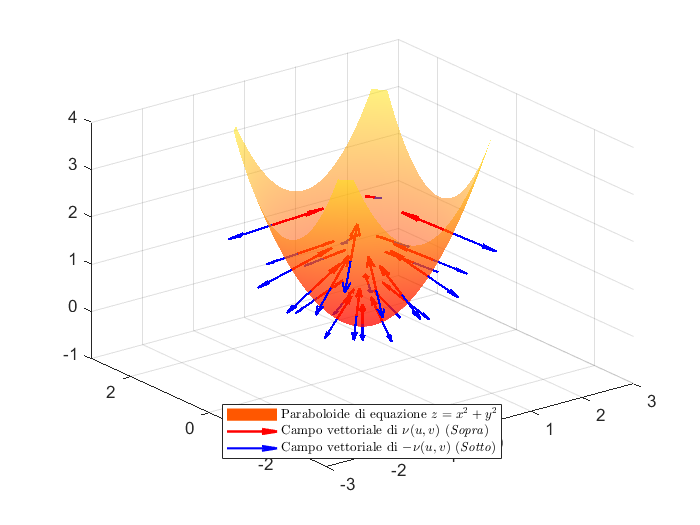
\includegraphics[width=\textwidth]{Capitoli/Capitolo6/Paraboloide.png}
    \end{minipage}
    \begin{minipage}{0.5\textwidth}
    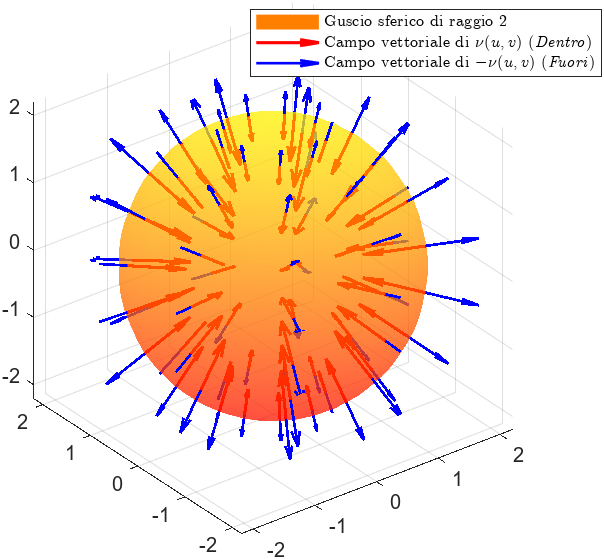
\includegraphics[width=\textwidth]{Capitoli/Capitolo6/Guscio sferico.png}
    \end{minipage}
    \begin{minipage}{0.4\textwidth}
    Discorso analogo, rispetto al "dentro" o "fuori" può essere fatto con un guscio sferico di raggio $R$ fissato. In figura $R=2$ con una superficie di parametrizzazione
    \begin{align*}
    r(u,v)=\begin{cases}
        x= R \sin u \cos v\\
        y= R \sin u \sin v\\
        z= R \cos u
    \end{cases}    
    \end{align*}
    con $u \in [0, 2\pi],\ v \in [0, \pi]$.
    \end{minipage}
    \end{figure}
 \end{example}
\section{Integrali superficiali}\cleardoublepage
\chapter{Successioni e serie di funzioni}
Il capitolo tratterà lo studio di successioni e serie di funzioni. I due argomenti sono tra loro collegati. Tuttavia, sebbene si possa ricondurre lo studio di una serie a quello di una successione, la successione delle ridotte n-esime, il capitolo non le porterà avanti in parallelo ma le analizzerà una per volta.
\section{Successioni di funzioni}
\begin{definition} \label{Def: Successione di funzioni}
     Si dice \textbf{successione di funzioni} l'insieme $\{\fn\}_{n \in \N}$ con
     \begin{equation}
         \fn: I \subseteq \R \to \R, n \in \N
     \end{equation}
\end{definition}
\begin{oss}
    Per questioni di praticità, laddove sia utilizzata una successione di funzioni, questa verrà indicata con $\fn$ anziché con $\{\fn\}_n\in \N$.
\end{oss}
Definito il concetto di successione di funzioni, si può iniziare a studiare la convergenza nelle sue diverse forme.\\
Innanzitutto, si noti che, fissato $\overline{x}\in I$, 
allora $\{\fn(\overline{x})\}_{n \in \N}$ è una successione numerica.
\begin{definition} \label{Def: Convergenza puntuale succ}
    Sia $\fn$ una successione di funzioni $I\to \R$. Allora si dice che $\fn$ \textbf{converge puntualmente} alla funzione $f: I \to \R$ se per ogni $\overline{x} \in I$ si ha che
    \begin{equation}
        \lim_{n \to +\infty} \fn(\overline{x}) = f(\overline{x})
    \end{equation}
    cioè
    \begin{equation}
        \forall\ \overline{x} \in I,\ \forall\ \varepsilon > 0,\ \exists\ N_{\varepsilon, x} \in \N\ \text{tale che}\ \forall\ n> N_{\varepsilon,x}\ \text{si ha}\ \left| \fn(x)-f(x)\right| < \varepsilon
    \end{equation}
    o, equivalentemente, sfruttando il criterio di Cauchy puntuale, se
\begin{equation}
    \forall\ x \in I, \forall\ \varepsilon > 0\ \exists\ N_{\varepsilon, x} \in N\ \text{tale che}\ \forall\ n,m > N_{\varepsilon, x}\ \text{si ha che}\ |\fn - f_m|<\varepsilon
\end{equation}
\end{definition}    
\begin{definition} \label{Def: Funzione limite}
    Inoltre, se c'è convergenza puntuale in $I$, è ben definita la \textbf{funzione limite} $f: I \to \R$ tale che
    \begin{equation}
        f(x) := \lim_{n \to +\infty} \fn(x)
    \end{equation}
\end{definition}
Nel caso della convergenza puntuale, $N$ dipende e da $\varepsilon$ e da $x$, pertanto può essere utile dare una definizione più forte di convergenza che non dipenda da $x$.
\begin{definition} \label{Def: Convergenza uniforme succ}
    Si dice che $\fn$ \textbf{converge uniformemente} su $I$ a $f: I \to \R$ se
    \begin{equation}
        \forall\ \varepsilon>0\ \exists\ N_\varepsilon \in \N\ \text{tale che}\ \forall\ n>N_\varepsilon\ \text{si ha}\ \sup_{x \in I}|\fn(x)-f(x)| < \varepsilon
    \end{equation}
    cioè se
    \begin{equation}
    \lim_{n \to + \infty}{\sup_{x \in I} \left| \fn(x)-f(x)\right|}=0
    \end{equation}
    o, tramite il criterio di Cauchy uniforme,
    \begin{equation}
        \forall \ \varepsilon >0 \ \exists\ N_\varepsilon \in \N \ \text{tale che}\ \forall\ n,m > N_\varepsilon\ \text{si ha}\ \sup_{x \in I}{|\fn(x)-f_m(x)|}<\varepsilon
    \end{equation}
\end{definition}
\begin{figure}[H]
    Graficamente, la convergenza uniforme fa sì che si verifichi una situazione di questo tipo.
    \centering
        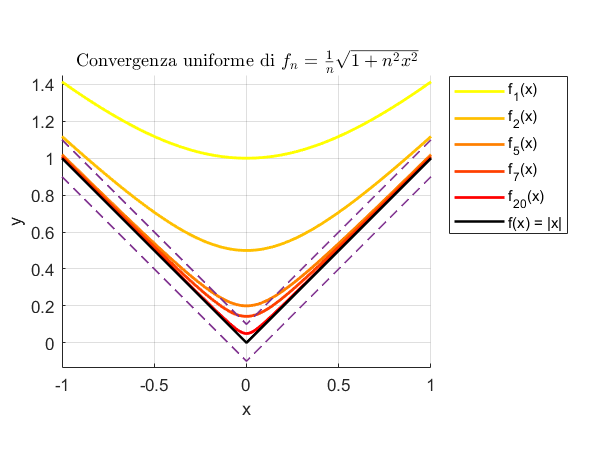
\includegraphics[width=0.39\textwidth]{Capitoli/Capitolo7/Convergenza uniforme.png}
\end{figure}
\begin{oss}
   Si può notare che la convergenza uniforme implica la convergenza puntuale, ma non è necessariamente vero il contrario.
    \end{oss}
\begin{oss}
 Per stabilire l'uniforme convergenza di una successione di funzioni, si può agire in due modi:
    \begin{itemize}
       \item Calcolare $\sup\limits_{x \in I} |\fn(x)-f(x)|$ ricercando massimi e minimi con gli strumenti del calcolo in una variabile.
       \item Maggiorare opportunamente $\sup\limits_{x \in I} |\fn(x)-f(x)|$.
\end{itemize}
\end{oss}
\begin{example}
Si studi ora la convergenza della seguente successione di funzioni, il cui grafico è riportato in figura
\begin{equation*}
    \fn= x^n, \qquad x \in [0,1]
\end{equation*}
Per quanto riguarda la convergenza puntuale si osserva che, fissato $x \in [0,1]$,
\begin{equation*}
    \lim_{n \to +\infty}{\fn(x)}= \lim_{n \to + \infty}= f(x) = \begin{cases}
        0 &\quad x \in [0,1]\\
        1 &\quad x=1
    \end{cases}
\end{equation*}
Volendo poi studiare la convergenza uniforme, si ha che
\begin{equation*}
    \sup_{x \in [0,1]}{\left|\fn(x)-f(x)\right|} = \sup_{x \in [0,1]} \left\{ \sup_{x \in [0,1)} \left|\fn(x)-f(x)\right|, \left|\fn(x)-f(x)\right|\right\} = \sup_{x \in [0,1)}{\left|x^n-0\right|} = 1 \neq 0
\end{equation*}
Dunque in $[0,1]$ $\fn$ non converge in modo uniforme. D'altra parte è anche vero che la "patologia" si verifica in $x=1$, perciò valutando la convergenza uniforme in $[0,a],\ a < 1$, si ha che
\begin{equation*}
    \sup_{x \in [0,a]}{|\fn(x)-f(x)|}= x^n \big|_{[0,a]} = a^n \overset{n \to +\infty}{\to} 0
\end{equation*}
cioè $\fn$ uniformemente convergente a $0$ su ogni compatto $[0,a],\ a<1$.\\
È possibile avere un riscontro grafico di tali affermazioni dalla figura di seguito.
\begin{figure}[H]
    \centering
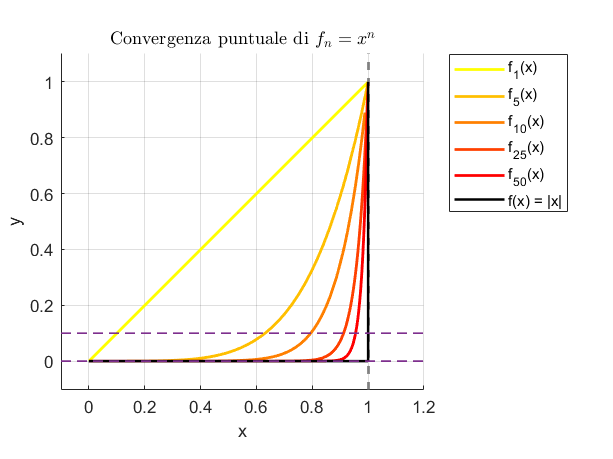
\includegraphics[width=0.55\textwidth]{Capitoli/Capitolo7/Convergenza puntuale.png}
    \end{figure}
\end{example}
\begin{theorem}[Scambio di limiti] \label{Teo: Scambio di limiti}
Sia $\fn: I \to \R$ tale che $\{\fn\}_n$ converge uniformemente in $I$ a $f: I \to \R$. Sia $x_0$ un punto di accumulazione per $I$ e si supponga che per ogni $n \in \N$ esista
\begin{equation}
    \ell_n:= \lim_{x \to x_0}{\fn(x)} \in \R
\end{equation}
Allora esistono i seguenti limiti e si ha
\begin{equation}
    \lim_{n \to +\infty}{\left(\lim_{x \to x_0} {\fn(x)}\right)}= \lim_{n \to +\infty}{\ell_n} = \lim_{x \to x_0} {f(x)} = \lim_{x \to x_0}{ \left( \lim_{n \to +\infty} {\fn(x)}\right)}
\end{equation}
\end{theorem}
\begin{proof}
    Si mostri che $\ell_n$ è una successione di Cauchy.\\
    Dalla convergenza uniforme delle $f_n$ si ha che
    \begin{equation}
        \forall\ \varepsilon>0\ \exists\ N_\varepsilon \in \N\ \text{tale che}\ \left| \fn(x)-f(x)\right|< \varepsilon,\ \forall\ x \in I
    \end{equation}
    Perciò, passando al limite per $x \to x_0$, si ha che
    \begin{equation}
        \left| \lim_{x \to x_0}{\fn(x)}-\lim_{x \to x_0}{f(x)}\right| = \left| \ell_n - \ell_m \right| \leq \varepsilon
    \end{equation}
    cioè $\ell_n$ è di Cauchy. Inoltre, $\{\ell_n\}_n$ è una successione di numeri reali, dunque essa deve convergere ad un qualche $\ell \in \R$. Ciò dimostra la prima metà della tesi.\\
    Rimane da provare che $f(x) \overset{x \to x_0}{\to} \ell$, cioè che $|f(x)-\ell| \to 0$. Dunque,
    \begin{equation}
    \begin{aligned}
        \left|f(x)-\ell\right| &= \left| f(x) - f_\nu(x)+ f_\nu(x)- \ell_\nu+ \ell_\nu- \ell\right| \leq\\
        &\overset{\text{Triang.}}{\leq} \left| f(x) - f_\nu(x) \right| +\left| f_\nu(x)- \ell_\nu(x)\right|+\left|\ell_\nu-\ell\right|
    \end{aligned}
    \end{equation}
    Si può notare che il primo termine è minore di $\varepsilon$ per ogni $\nu > N_\varepsilon$ per convergenza uniforme e che il terzo, essendo una successione numerica, è minore di $\varepsilon$ per un $\nu$ sufficientemente grande, poiché $\ell_n \to \ell$. Il secondo, fissato $\nu$ come sopra, soddisfa per ipotesi
    \begin{equation}
        \lim_{x \to x_0}{f_\nu(x)} = \ell_\nu
    \end{equation}
    Dunque, esiste un intorno $\U(x_0)$ tale che per ogni $x \in \U(x_0)$, $\left| f_\nu(x)- \ell_\nu \right| < \varepsilon$.\\
    In conclusione, per $\nu$ fissato come sopra e $x \in \U(x_0)$ si ha che
    \begin{equation}
        \left|f(x)-\ell\right| < 3 \varepsilon
    \end{equation}
\end{proof}
\begin{oss}
    Il passaggio al limite nella prima parte della dimostrazione è consentito dal fatto che per ipotesi siano definite $\ell_n$ e $\ell_m$ reali.
\end{oss}
Da tale teorema discende come conseguenza immediata il seguente corollario
\begin{corollary} \label{Cor: Corollario a scambio limiti}
    Sia $\fn$ una successione di funzioni continue uniformemente convergente in $I$ a $f:I \to \R$. Allora $f$ è continua. 
\end{corollary}
\begin{proof}
    Si mostri che preso $x_0$ punto di accumulazione per $I$, si ha
    \begin{equation}
        \lim_{x \to x_0}{f(x)}= f(x_0)
    \end{equation}
    Dunque sfruttando l'ipotesi di convergenza, si ha che
    \begin{equation}
        \lim_{x \to x_0}{\fn(x)}= \fn(x_0) \in \R
    \end{equation}
    D'altra parte vale lo scambio di limiti, quindi
    \begin{equation}
    \begin{aligned}
          f(x_0) &=  \lim_{n \to +\infty}{\fn(x_0)}= \lim_{n \to +\infty}{\left(\lim_{x \to x_0}{\fn(x)}\right)}=\\
          &= \lim_{x \to x_0}{ \left( \lim_{n \to +\infty}{\fn(x)}\right)}=\lim_{x \to x_0}{f(x)} 
    \end{aligned}
    \end{equation}
\end{proof}
Vista tale proprietà dei limiti, può essere ragionevole porsi lo stesso dubbio per le derivate e gli integrali. A tal proposito, si mostrino ora due importanti risultati rispetto alla derivazione e all'integrazione di successioni di funzioni.
\begin{theorem}[Teorema di passaggio al limite sotto al segno di derivata] \label{Teo: Passaggio al limite sotto al segno di derivata}
    Sia $\{\fn\}_{n\in\N}$ una successione di funzioni $C^1[a,b]$. Sia la successione di numeri reali $\{\fn(x_0)\}_n$ convergente e sia $\{\fn'\}_n$ uniformemente convergente. Allora $\{\fn\}_n$ converge uniformemente in $[a,b]$ ad una funzione $f \in C^1([a,b])$ e 
    \begin{equation}
        \lim_{n \to +\infty}{\fn'(x)}= \left(\lim_{n \to +\infty}{\fn(x)}\right)'=f'(x)
    \end{equation}
\end{theorem}
\begin{theorem}[Teorema di passaggio al limite sotto al segno di integrale] \label{Teo: Passaggio al limite sotto al segno di integrale}
Sia $\{\fn\}_{n_\in \N}$ una successione di funzioni continue in $[a,b]$ uniformemente convergente in $[a,b]$ a $f$. Allora
\begin{equation}
    \lim_{n \to +\infty}{\int\limits_{a}^{b}{\fn(x)}\,dx}=\int\limits_{a}^{b}{\lim_{n \to +\infty}{\fn(x)}\,dx}= \int\limits_{a}^{b}{f(x)}\,dx
\end{equation}
\end{theorem}
\begin{example}
    In questo esempio si può osservare quanto sia rilevante l'ipotesi di uniforme convergenza della successione.
    \begin{figure}[H]
        \centering
        \begin{minipage}{0.5\textwidth}
            Si consideri la successione di funzioni data da 
            \begin{equation*}
            f_n(x)=\begin{cases}
            0 &\qquad x=0\\
            n & \qquad x \in (0, \frac{1}{n})\\
            0 &\qquad x \in (\frac{1}{n}, 1)\\
            \end{cases}
            \end{equation*}
            e si osservi che
            \begin{equation*}
                \int\limits_{0}^{1}{\fn(x)}\,dx=1 \neq \int\limits_{0}^{1}{f(x)}\,dx = 0
            \end{equation*}
        \end{minipage}
        \begin{minipage}{0.4\textwidth}
        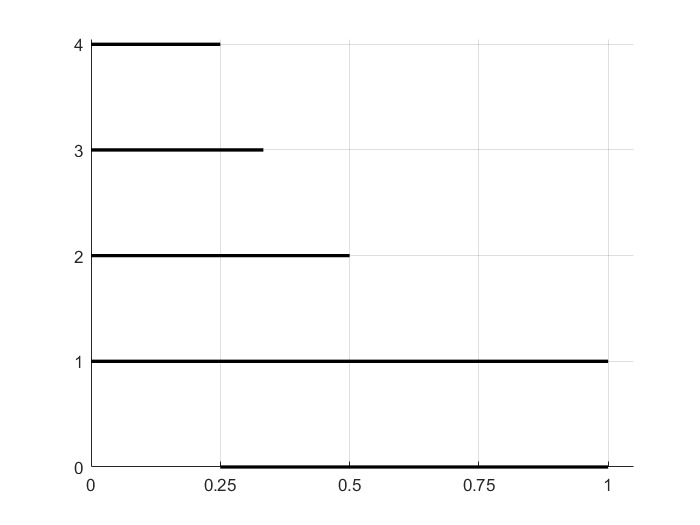
\includegraphics[width=\textwidth]{Capitoli/Capitolo7/Esempio integrale succ. funz..png}
        \end{minipage}
    \end{figure}
    poiché non uniformemente convergente.
\end{example}
\section{Serie di funzioni}
Quando si parla di serie, ci si può rifare alle successioni. Perciò in questa sezione verranno rielaborate le informazioni del capitolo precedente adattandole alle serie di funzioni.
\begin{definition}
    Sia $\{\fn\}_{n \in \N}$ una successione di funzioni, $\fn: I \subseteq \R \to \R$. Si dice \textbf{serie di funzioni} di termine generale $\fn$ la successione di funzioni delle somme parziali di $\{\fn\}_{n \in \N}$ data da
    \begin{equation}
        \sn(x)=\sum\limits_{n=1}^{N}{\fn(x)}
    \end{equation}
\end{definition}
\begin{definition}
    Sia $\sum\limits_{n=1}^{\infty}{\fn(x)}$ una serie di funzioni. Allora si dice che la serie \textbf{converge puntualmente} in I se la successione $\{\sn\}_{n \in \N}$ converge puntualmente in I. In maniera equivalente, la serie converge se, detta
    \begin{equation}
        s(x)=\lim_{n \to +\infty}{\sn(x)}
    \end{equation}
    si ha che
    \begin{equation}
        \forall\ x \in I,\ \forall\ \varepsilon>0,\ \exists\ N_{\varepsilon, x}\ \text{tale che}\ \forall N>N_{\varepsilon, x}\ \text{si ha che}\ |\sn(x)-s(x)|< \varepsilon
    \end{equation}
    o, ancora, sfruttando il criterio di Cauchy, se
    \begin{equation}
        \forall\ x \in I,\ \forall\ \varepsilon>0,\ \exists\ N_{\varepsilon, x}\ \text{tale che}\ \forall\ n>N_{\varepsilon, x},\ \forall p \in \N\ \text{si ha}\ |f_{n+1}(x)+ \dots+ f_{n+p}(x)|<\varepsilon
    \end{equation}
\end{definition}
\begin{definition}
    Se la serie converge puntualmente è ben definita la funzione \textbf{somma}
    \begin{equation}
        s(x)=\lim_{n \to +\infty}{\sn(x)}= \sum_{n=0}^{\infty}{\fn(x)}
    \end{equation}
\end{definition}
\begin{definition}
Sia $\sum\limits_{n=1}^{\infty}{\fn(x)}$ una serie di funzioni. Allora si dice che la serie \textbf{converge uniformemente} in I se la successione $\{\sn\}_{n \in \N}$ converge uniformemente in I. In maniera equivalente, sfruttando il criterio di Cauchy uniforme, se
\begin{equation}
\forall\ \varepsilon>0\ \exists\ N_\varepsilon \in \N\ \text{tale che}\ \forall\ n > N_\varepsilon\ \forall\ p \in \N\ \text{si ha}\ \sup_{x \in I}{|f_{n+1}(x)+\dots+f_{n+p}(x)|}<\varepsilon 
\end{equation}
\end{definition}
\begin{definition}
    Sia $\{\sn\}_{n \in \N}$ una serie di funzioni. Si dice che la serie \textbf{converge assolutamente}  se
    \begin{equation}
        \sum_{n}{|\fn(x)|}
    \end{equation}
    converge per ogni $x \in I$
\end{definition} 
\begin{oss}
Valgono le seguenti relazioni tra le varie nozioni di convergenza per le serie:
\begin{itemize}
    \item Convergenza assoluta $\Rightarrow$ Convergenza puntuale.
    \item  Nessuna correlazione tra convergenza assoluta e convergenza uniforme.
\end{itemize}
\end{oss}
\begin{example}
    La convergenza puntuale non implica la convergenza assoluta. Infatti, sia
    \begin{equation*}
        \fn(x)=\frac{(-1)^n}{n}
    \end{equation*}
    Allora $\sum\limits_{n}{\fn}$ converge ma $\sum\limits_{n}{|\fn|}$ diverge.
\end{example}
\begin{definition}
    Sia $\sum\limits_{n=1}^{\infty}{\fn(x)}$ una serie di funzioni. Si dice che essa converge totalmente in $I$ se esiste una successione numerica $\{k_n\}_n$ con $k_n>0$ per ogni $n$ tale che
    \begin{enumerate}
        \item $|\fn|<k_n$
        \item $\sum\limits_{n}{k_n}$ converge
    \end{enumerate}
\end{definition}
\begin{proposition}
    Una serie totalmente convergente è assolutamente convergente.
\end{proposition}
\begin{proof}
    Se $\sum\limits_{n}\fn$ converge totalmente, allora per definizione esiste una successione $k_n$ tale che $|\fn|<k_n$ e tale che la propria serie converga. Ma allora si ha che
    \begin{equation}
        \sum_{n}{|\fn|} < \sum_{n}{k_n}= \ell \in \R
    \end{equation}
    Perciò, per il teorema del confronto per le serie, $\sum\limits{|\fn|}$ converge e, quindi, $\sum\limits{\fn}$ converge assolutamente.
\end{proof}
\begin{theorem}[Criterio di Weierstrass] \label{Teo: Criterio di Weierstrass (convergenza totale)}
Una serie di funzioni $\sum\limits_{n=1}^{\infty}{\fn(x)}$ totalmente convergente in $I$ è ivi uniformemente convergente.
\end{theorem}
\begin{proof}
    Si sfrutti il criterio di Cauchy uniforme per le serie. L'obiettivo quindi è mostrare che esista un $N_\varepsilon$ tale che $|f_{n+1}+ \dots+ f_{n+p}|< \varepsilon,\ \forall\ n > N_\varepsilon,\ \forall\ p\in \N$.\\
    Dunque, si fissi $\varepsilon>0$. Per ipotesi di convergenza totale si ha che $\sum\limits_{n=1}^{\infty}{k_n}$ converge. Allora, esiste un $N_\varepsilon>0$ tale che per ogni $n>N_\varepsilon$ si ha che 
    \begin{equation}
        |k_{n+1}+\dots+k_{n+p}|< \varepsilon \qquad \forall\ p \in \N
    \end{equation}
   con $k_n>0\ \forall\ n$.\\
   D'altra parte, $|\fn|<k_n$ e, di conseguenza, a patto di prendere $n> N_\varepsilon$ si ha che, $\forall\ p \in \N,\ \forall x \in I$, vale
    \begin{equation}
    \begin{aligned}
        |f_{n+1}(x)+ \dots + f_{n+p}(x)| &\leq |f_{n+1}(x)|+ \dots + |f_{n+p}(x)|<\\ 
        &< k_{n+1}+ \dots + k_{n+p} < \varepsilon
    \end{aligned}
    \end{equation}
    Dunque è verificato il criterio di Cauchy uniforme e la serie converge uniformemente in I.
\end{proof}
\begin{oss}
    Il teorema offre una condizione sufficiente per la convergenza uniforme.
\end{oss}
\begin{oss}
Per quanto visto, una serie $\sum\limits_{n}{\fn(x)}$ converge totalmente se e solo se $\sum\limits_{n}{\sup\limits_{x \in I}{|\fn(x)|}} < +\infty$. Infatti, se in tale contesto esiste una $k_n \geq |\fn(x)|$ per ogni $n$ la cui serie converge, allora è soddisfatta la definizione di convergenza totale.\\
Anche qui si può operare in due modi:
\begin{itemize}
    \item Calcolare $\sup\limits_{x \in I}{|\fn(x)|}$.
    \item Maggiorare opportunamente $\sup\limits_{x \in I}{|\fn|}$.
\end{itemize}
\end{oss}
Con le dovute modifiche all'enunciato, valgono per le serie i teoremi \ref{Teo: Scambio di limiti}, \ref{Cor: Corollario a scambio limiti}, \ref{Teo: Passaggio al limite sotto al segno di derivata} e \ref{Teo: Passaggio al limite sotto al segno di integrale} mostrati nella sezione precedente.
\begin{theorem}[Teorema di scambio dei limiti per le serie di funzioni]
    Sia $\fn: E \subseteq \R \to \R$ e sia $x_0$ di accumulazione per $E$. Se esiste finito
    \begin{equation}
        \lim_{x \to x_0}{\fn(x)} \qquad \forall\ n\geq0
    \end{equation}
    e se $\sum\limits_{n=0}^{\infty}{\fn(x)}$ converge uniformemente su E alla somma $S(x)$, allora $S(x)$ converge per $x \to x_0$ e 
    \begin{equation}
        \lim_{x \to x_0}{S(x)= \sum\limits_{n=0}^{\infty}{\lim_{x \to x_0}{\fn(x)}}}
    \end{equation}
\end{theorem}
\begin{theorem}
    Siano $I \subseteq \R,\ \fn \in C^0(I)$ e sia $\sum\limits_{n=0}^{\infty}{\fn(x)}$ uniformemente convergente in $I$ a $s$. Allora la funzione somma $s(x)$ è continua in $I$.
\end{theorem}
\begin{theorem}
    Sia $\fn \in C^1([a,b])$ e si supponga $\sum\limits_{n=0}^{\infty}{\fn(x)}$ puntualmente convergente in $[a,b]$ a $s(x)$ e $\sum\limits_{n=0}^{\infty}{\fn'(x)}$ uniformemente convergente in $[a,b]$. Allora
    \begin{equation}
        \sum\limits_{n=0}^{\infty}{\fn'(x)}= 
        \left(\sum\limits_{n=0}^{\infty}{\fn(x)}\right)'= s'(x) \qquad \forall\ x \in [a,b]
    \end{equation}
\end{theorem}
\begin{theorem}
    Sia $\fn \in C^0([a,b])$ e sia $\sum\limits_{n=0}^{\infty}{\fn(x)}$ uniformemente convergente in $[a,b]$ a $s$. Allora
    \begin{equation}
        \sum\limits_{n=0}^{\infty}{\int\limits_{a}^{b}{\fn(x)}\, dx}= \int\limits_{a}^{b}{\sum\limits_{n=0}^{\infty}{\fn(x)}\, dx}= \int\limits_{a}^{b}{s(x)}\, dx
    \end{equation}
\end{theorem}
\section{Serie di potenze}
\begin{definition}
Si dice \textbf{serie di potenze} reale di centro $x_0 \in \R$ una serie di funzioni della forma
\begin{equation}
    a_0+ \sum_{n=1}^{\infty}{a_n(x-x_0)^n} \qquad a_n \in \R\ \forall\ n=0,1,\dots
\end{equation}
\end{definition}
\begin{oss}
    Mediante opportune traslazioni è possibile passare da una serie di potenze centrata in $x_0$ a una centrata in $0$ della forma
    \begin{equation}
        \sum_{n=0}^{\infty}{a_n x^n}
    \end{equation}
\end{oss}
\begin{definition}
    Si dice \textbf{raggio di convergenza} della serie $\sum\limits_{n=0}^{\infty}{a_n x^n}$ l'estremo superiore $R$ dell'insieme $E$ dei numeri reali $\xi$ nei quali la serie converge, ossia
    \begin{equation}
        R= \sup E \qquad E=\left\{ \xi \in \R \mid \sum_{n=0}^{\infty}{a_n x^n}\ \text{converge}\right\}
    \end{equation}
\end{definition}
La caratterizzazione di $R$ si ha a partire dal seguente teorema.
\begin{theorem} \label{Teo: Caratterizzazione del raggio di convergenza}
    Sia $R$ raggio di convergenza della serie di potenze. Se $R=0$, allora la serie converge solo in $0$. Se $R>0$, la serie converge totalmente in ogni $[a,b] \subset (-R, R)$ e non converge per $|x|>R$.
\end{theorem}
\begin{proof}
 Si mostri che se $\sum\limits_{n=0}^{\infty}{a_n \xi^n}$ converge per un qualche $\xi \neq 0$ allora converge totalmente in ogni intervallo $[-\eta, \eta] \subset (-|\xi|, |\xi|)$.\\
 Per ipotesi di convergenza della serie, $|a_n \xi^n|$ deve essere una successione infinitesima (e perciò limitata) per $n\to +\infty$, ovvero
 \begin{equation}
     \exists\ M>0\ \text{tale che}\ |a_n\xi^n|\leq M
 \end{equation}
 A questo punto, fissato $\eta>0$ tale che $\eta<|\xi|$, si calcoli il termine generale della serie per un qualche $x \in [-\eta, \eta]$.
 \begin{equation}
     |a_n x^n| = \left|a_n x^n \frac{\xi^n}{\xi^n}\right|=\left|a_n \xi^n\right| \left|\frac{x}{\xi}\right|^n \leq M \left(\frac{|x|^n}{\left|\xi\right|^n} \right)\leq M \left(\frac{\eta}{\left| \xi \right|} \right)^n =k_n
 \end{equation}
 Poiché $k_n$ è il termine generale di una serie geometrica di ragione $\left(\tfrac{\eta}{\left| \xi \right|} \right)^n < 1$, essa è convergente. Quindi
 \begin{equation}
 \forall\ x \in [-\eta, \eta],\ \sum\limits_{n=0}^{\infty}{|a_n \xi^n|} \leq M \sum_{n=0}^{\infty}{\left(\frac{\eta}{\left| \xi \right|} \right)^n}
 \end{equation}
 che soddisfa le condizioni di convergenza totale con $k_n=\left(\tfrac{\eta}{\left| \xi \right|} \right)^n$.\\
 Nel caso in cui $R=0$, per quanto detto, la serie non può convergere in punti $\xi$ tali che $\xi \neq 0$.\\
 Nel caso in cui $|x|>R$, si ha che, per $x>R$ la serie non converge perché andrebbe in contraddizione con la definizione di $\sup$ propria di $R$; discorso analogo vale per $x<-R$, siccome la convergenza in tale punto implicherebbe la convergenza in ogni $[-\eta, \eta] \subset (-|x|, |x|)$ e, se così fosse, si contraddirebbe nuovamente la definizione di $\sup$.
\end{proof}
\begin{oss}
Il teorema dà un'ulteriore informazione: se $R= +\infty$, allora la serie di potenze converge totalmente in ogni compatto di $\R$.
\end{oss}
\begin{theorem}[Criterio di Cauchy-Hadamard] \label{Teo: Criterio di Cauchy-Hadamard}
Sia $\sum\limits_{n=0}^{\infty}{a_n x^n}$ una serie di potenze. Se esiste il limite
\begin{equation}
    \ell=\lim_{n \to +\infty}{\sqrt[n]{|a_n|}}
\end{equation}
    allora il raggio di convergenza vale
    \begin{equation}
        R = \begin{cases}
            +\infty &\qquad \ell=0\\
            \frac{1}{\ell} &\qquad \ell \neq 0\\
            0 &\qquad \ell = +\infty
        \end{cases}
    \end{equation}
\end{theorem}
\begin{proof}
    Per ogni $x \neq 0$ risulta
    \begin{equation}
        \lim_{n \to +\infty}{\sqrt[n]{|a_n x^n|}} = \ell|x| := L
    \end{equation}
    Allora, dallo studio di $\ell$ si ha che
    \begin{enumerate}
        \item $\ell=0 \Rightarrow L=0$, perciò, per criterio della radice delle serie numeriche, la serie converge assolutamente per ogni $x \neq 0$. Inoltre, poiché la serie converge anche con $x=0$, $R=+\infty$.
        \item $\ell= +\infty \Rightarrow L =+ \infty$, quindi, per ogni $x \neq 0$ la serie non converge assolutamente, cioè $R=0$.
        \item $0< \ell<+\infty$, per il criterio della radice delle serie numeriche, quando $L<1 \iff |x|< \tfrac{1}{\ell}$ la serie converge assolutamente. Invece, quando $L>1 \iff |x|>\tfrac{1}{\ell}$ la serie non converge assolutamente, quindi, $R= \tfrac{1}{\ell}$.
    \end{enumerate}
\end{proof}
Oltre al criterio della radice, vale anche il criterio del rapporto, di cui viene dato solo l'enunciato, dal momento che la sua dimostrazione è analoga a quella precedente con l'eccezione di applicare il criterio del rapporto per le serie numeriche anziché quello della radice.
\begin{theorem}[Criterio di d'Alembert]
    Sia $\sum\limits_{n=0}^{\infty}{a_n x^n}$ una serie di potenze. Se esiste il limite
    \begin{equation}
        \ell= \lim_{n \to \infty}{\frac{a_{n+1}}{a_n}}
    \end{equation}
    allora il raggio di convergenza della serie vale
    \begin{equation}
        R= \begin{cases}
        +\infty &\qquad \ell=0\\
        \frac{1}{\ell} &\qquad \ell \neq 0\\
        0 &\qquad \ell = \infty
        \end{cases}
    \end{equation}
\end{theorem}
Il teorema di Abel, che segue, offre una condizione sufficiente per la convergenza uniforme di serie di potenze.
\begin{theorem}[Teorema di Abel] \label{Teo: Teorema di Abel}
    Sia $\sum\limits_{n=0}^{\infty}{a_n x^n}$ una serie di potenze con raggio di convergenza $R$, con $0<R<+\infty$. Sia poi $M$ tale che $0<M<R$. Se la serie converge anche in $x=R$ (o $x=-R$) allora la serie converge uniformemente su $[-M, R]$ (o $[-R, M]$). \\
    In particolare, se la serie converge in $x= \pm R$, allora essa converge uniformemente in $[-R, R]$.
\end{theorem}
\subsection{Sviluppabilità di una funzione in serie di potenze}
\begin{theorem}[Derivazione di serie di potenze] \label{Teo: Derivazione di serie di potenze}
Sia $\sum\limits_{n=0}^{\infty}{a_n x^n}$ una serie di potenze con raggio di convergenza $R>0$. Sia poi $f$ la sua funzione somma. Allora la serie
\begin{equation}
    \sum\limits_{n=1}^{\infty}{\left(a_n x^n\right)'}= \sum\limits_{n=1}^{\infty}{n a_n x^{n-1}}= \sum\limits_{j=0}^{\infty}{\left(j+1\right)a_{j+1} x^j}
\end{equation}
ha lo stesso raggio di convergenza $R$. Inoltre, esiste $f'(x)\ \forall\ x \in (-R, R)$ e
\begin{equation}
    f'(x)=\sum\limits_{n=0}^{\infty}{\left(n+1\right)a_{n+1} x^n}
\end{equation}
\end{theorem}
\begin{proof}
    Per semplicità si supponga che esista e valga 
    \begin{equation}
        \lim_{n \to \infty}{\sqrt[n]{|a_n|}}=\frac{1}{R}
    \end{equation}
    e si calcoli il raggio di convergenza della serie derivata. Allora
    \begin{equation}
        \lim_{j \to + \infty}{\sqrt[j]{(j+1)|a_{j+1}|}} = \lim_{j \to + \infty}{\sqrt[j]{(j+1)}} \lim_{j \to + \infty}{\sqrt[j]{|a_{j+1}|}}= \lim_{j \to + \infty}{{\left(|a_{j+1}|^{\frac{1}{j+1}}\right)^{\frac{j+1}{j}}}}  \overset{\ref{Teo: Criterio di Cauchy-Hadamard}}{=} \frac{1}{R}
    \end{equation}
    E quindi, ponendosi in un compatto $[a,b] \subset (-R, R)$ in cui la serie derivata e la serie di potenze convergono totalmente e applicando il teorema, si ha la tesi.
\end{proof}
Reiterando tale procedimento, si può osservare che la somma della serie di potenze deve essere di classe $C^\infty$. Dunque, si può stabilire una condizione necessaria di buona approssimazione di una funzione $f$ tramite una serie di potenze, cioè il fatto che $f \in C^{\infty}$. Tale questione non si pone invece parlando di serie di Fourier.\\
D'altro canto, si possono introdurre ora le serie di Taylor. 
\begin{proposition}
Sia $x_0=0$ e sia $f \in C^\infty$ tale che in $(-R, R)$ si abbia
\begin{equation}
    f(x)= \sum\limits_{n=0}^{\infty}{a_n x^n}
\end{equation}
Allora tale serie è la serie di Taylor di $f$.
\end{proposition}
\begin{proof}
Per quanto detto nel teorema precedente, deve valere
\begin{equation}
    f^{(m)}(x)= \sum\limits_{n=m}^{\infty}{\frac{n!}{(n-m)!} a_n x^{n-m}}
\end{equation}
e quindi, ponendo $x=0$, tutti gli addendi dopo il primo si azzerano, lasciando così
\begin{equation}
    f^{(m)}(0)=a_n m! \Rightarrow a_n=\frac{f^{(m)}}{m!} \qquad \forall\ n
\end{equation}
cioè $a_n$ è il coefficiente di Taylor.
\end{proof}
\begin{definition} \label{Def: Funzione analitica}
    Si dice che una funzione $f$ è una funzione \textbf{analitica} in $\U(0)$ se sull'intervallo $(-\varrho, \varrho)$ si ha che
    \begin{equation}
        f(x)= \sum\limits_{n=0}^{\infty}{a_n x^n}
    \end{equation}
\end{definition}
\begin{oss}
    Esistono funzioni di classe $C^\infty$ la cui serie di Taylor abbia raggio di convergenza $R=0$.
\end{oss}
\begin{oss}
    La definizione di funzione analitica può essere formulata in un generico $\U(x_0)$ e si può dimostrare che se $f$ è analitica in $(x_0-\varrho, x_0+\varrho)$, allora lo è anche in un intorno di ogni $x_1 \in (x_0-\varrho, x_0+\varrho)$.
\end{oss}
\begin{theorem}
    Le funzioni analitiche sono un sottoinsieme proprio di $C^\infty$
\end{theorem}
\begin{proof}
 Si dimostri il teorema con un controesempio. Sia 
 \begin{equation}
     f(x)= \begin{cases}
         e^{-\frac{1}{x^2}} &\qquad x \neq 0\\
         0 &\qquad x=0
     \end{cases}
 \end{equation}
 Tale funzione è continua in $\R$ e verifica 
 \begin{equation}
     \lim_{x \to 0}{f(x)}=0= \lim_{x \to 0}{ e ^{-\frac{1}{x^2}}}
 \end{equation}
 Allora, calcolandone la derivata prima si ha 
 \begin{equation}
     f'(x)= \begin{cases}
         \frac{2}{x^3} e^{-\tfrac{1}{x^2}} & \qquad x \neq 0\\
         \lim\limits_{x \to 0}{\frac{f(x)-f(0)}{x}}= \lim\limits_{x \to 0}{\frac{e^{-\frac{1}{x^2}}}{x}}=0 &\qquad x=0
     \end{cases}
 \end{equation}
 Continuando a derivare, si ottiene sempre un'equazione del tipo
 \begin{equation}
     f^{(m)}(x)=\begin{cases}
         C e^{-\frac{1}{x^2}} &\qquad x\neq0\\
         0 &\qquad x=0
     \end{cases}
 \end{equation}
 cioè, $f \in C^\infty(\R)$. Tuttavia, $f^{(m)}(0)=0$. Pertanto la serie di Taylor dovrebbe essere la funzione nulla, ma $f \not\equiv 0\ \forall\ x \in \dot{\U}(0)$, quindi non è analitica.
\end{proof}
Allora, per terminare, si dia ora un criterio per stabilire se una funzione sia sviluppabile come serie di potenze.
\begin{theorem}[Criterio di sviluppabilità] \label{Teo: Criterio di sviluppabilità}
    Sia $f \in C^\infty(-\varrho, \varrho)$ per un qualche $\varrho>0$. Sia poi
    \begin{equation}
        \sup_{x \in (-\varrho, \varrho)}{|f^{n}(x)|}\leq L^{n+1}n!
    \end{equation}
    per un'opportuna costante $L>0$. Allora $f$ è analitica in un intorno $\U(0)$
\end{theorem}
\begin{oss}
    Funzioni come $e^x,\ \sin(x), \ \cos(x)$ sono analitiche.
\end{oss}
\section{Spazi metrici}
\begin{definition} \label{Def: Spazi metrici}
    Sia $X$ un insieme e sia $d$ una metrica (\ref{Def: Distanza}). Si dice \textbf{spazio metrico} la coppia $\left(X, d\right)$
\end{definition}
\begin{example}
    Esempi di spazi metrici possono essere:
    \begin{itemize}
        \item $X=\R^n$ con distanza euclidea $d(x, y):= \sqrt{ \sum\limits_{i=1}^n{(x_i-y_i)^2}}$.
        \item $X=\R^n$ con $d_\infty(x,y):= \max\limits_{i=1, \dots, n}{|x_i-y_i|}$.
        \item $X=C^0([a,b], d_\infty)$ con $d_\infty(x,y):= \sup\limits_{x \in [a,b]}{|f(x)-g(x)|}$. 
    \end{itemize}
\end{example}
\begin{definition} \label{Def: Palla di raggio r}
    Sia $(X, d)$ uno spazio metrico. Si dice \textbf{palla} di raggio $r$ centrata in $x_0$ l'insieme
    \begin{equation}
    B_r(x_0)= \left\{ x \in X \mid d(x_0, x)< r\right\}
    \end{equation}
\end{definition}
\begin{definition} \label{Def: Convergenza e convergenza di Cauchy}
Una successione $\{x_n\}_n$ con $x_n \in (X, d)$ per ogni n e con $(X, d)$ spazio metrico \textbf{converge} a $x_0 \in X$ se
\begin{equation}
    d(x_n, x_0) \overset{n \to +\infty}{\to} 0
\end{equation}
Inoltre, se 
\begin{equation}
    \forall\ \varepsilon>0\ \exists\ N_\varepsilon\ \text{tale che}\ \forall\ n,m > N_\varepsilon\ \text{si ha}\ d(x_n, x_m)< \varepsilon
\end{equation}
allora tale successione è detta \textbf{di Cauchy}.
\end{definition}
\begin{definition} \label{Def: Spazio metrico completo}
    Uno spazio metrico $(X, d)$ è detto \textbf{completo} se ogni successione di Cauchy in X converge ad un elemento di X.
\end{definition}
\begin{example}
    Esempi di spazi metrici completi possono essere
    \begin{itemize}
        \item $X=\R^n$ con distanza euclidea o con $d_\infty$.
        \item $X=\R^n$ con $d_p= \left(\sum\limits_{i=1}^{n}{|x_i - y_i|^p}\right)^{\frac{1}{p}}$ e $p\geq 1$. (Nota: per $p=2$, la distanza $d_p$ è la distanza euclidea).
    \end{itemize}
    Uno spazio metrico non completo è invece $\mathbb{Q}^n$.
\end{example}
\begin{oss}
    Uno spazio vettoriale normato ($\Rightarrow$ metrico con $d(x, y)= |x-y|$) completo è detto spazio di \textbf{Banach}.\\
    Se in aggiunta la norma di tale spazio discende da un prodotto scalare, esso è detto spazio di \textbf{Hilbert}.
\end{oss}
\begin{theorem}
    $(C^0([a,b]), d_\infty)$ è uno spazio metrico completo.
\end{theorem}
\begin{proof}
    Sia $\{\fn\}_n$ di Cauchy in $(C^0([a,b]), d_\infty)$. Allora, 
    \begin{equation}
          \forall\ \varepsilon>0\ \exists\ N_\varepsilon\ \text{tale che}\ \forall\ n,m > N_\varepsilon\ \text{si ha}\ d(\fn, f_m)< \varepsilon
    \end{equation}
    cioè 
    \begin{equation}
     \sup\limits_{x \in [a,b]}{|\fn(x)-f_m(x)|}< \varepsilon
    \end{equation}
    Ma allora $\fn$ soddisfa il criterio di Cauchy uniforme ed esiste una funzione limite $f$ cui $\fn$ converge uniformemente in $[a,b]$ per $n \to \infty$. Poiché poi $\fn$ sono continue per ipotesi e convergono uniformemente ad $f$, sono soddisfatte le ipotesi del corollario \ref{Cor: Corollario a scambio limiti}, quindi $f \in C^0([a,b], d_\infty)$.
\end{proof}
\begin{oss}
    Si può notare che la definizione di completezza dipende dalla distanza. A tal proposito si consideri lo spazio metrico $(C^0([-1,1], d_p)$ con 
    \begin{equation*}
        d_p=\left(\int\limits_{-1}^{1}{|f(x)-g(x)|^p\, dx}\right)^\frac{1}{p}
    \end{equation*}
    e si prenda la successione
    \begin{equation*}
        \fn(x) = \begin{cases}
            -1 &\qquad x \in [-1, -\frac{1}{n}]\\
            nx &\qquad x \in [-\frac{1}{n}, \frac{1}{n}]\\
            1 &\qquad x \in [\frac{1}{n}, 1]
        \end{cases}
    \end{equation*}
    Il suo limite è
    \begin{equation*}
        f(x)= \sgn(x)=\begin{cases}
            -1 &\qquad x \in [-1,0)\\
            0 &\qquad x =0\\
            1 &\qquad x \in (0, 1]
        \end{cases}
    \end{equation*}
    e $f\notin C^0([-1, 1])\ \forall\ x$
    benché $\fn$ sia di Cauchy. Infatti, 
    \begin{equation*}
        d_p(\fn, f)=  d_p=\left(\int\limits_{-1}^{1}{|\fn-f|^p\, dx}\right)^\frac{1}{p} \leq \left(\int\limits_{-\tfrac{1}{n}}^{\tfrac{1}{n}}{2^p\, dx}\right)^\frac{1}{p} \overset{n \to \infty}{\to }0
    \end{equation*}
\end{oss}
\begin{definition} \label{Def: Spazio chiuso}
    Sia $(X, d)$ metrico. Un sottoinsieme $C \subset X$ è detto \textbf{chiuso} se ogni successione $\{x_n\}_n$ di elementi di $C$ che converge rispetto a $d$, converge ad un elemento di $C$.
\end{definition}
\begin{theorem} \label{Teo: Sottospazio chiuso di un completo è completo}
    Sia $(X,d)$ uno spazio metrico completo e $C \subset X$ chiuso. Allora $(C, d)$ è un sottospazio metrico completo.
\end{theorem}
\begin{proof}
    Sia $\{x_n\}_n$ una successione di Cauchy in $C$. Poiché $x_n \in C \subset X$ e $X$ è metrico completo, 
    \begin{equation}
        \exists\ y \in X\ \text{tale che}\ d(x_n, y)\to 0
    \end{equation}
    D'altra parte $x_n$ è una successione di $C$, che è chiuso. Dunque, per definizione, $y \in C$, cioè $C$ è metrico completo.
\end{proof}
\begin{definition} \label{Def: Funzione sequenzialmente continua}
    Siano $(X, d_x),\ (Y, d_y)$ spazi metrici. Allora $f: X \to Y$ è detta \textbf{sequenzialmente continua} in $x_0 \in X$ se per ogni successione $\{x_n\}_n \subset X$ tale che $x_n \overset{n\to +\infty}{\to} x_0$ rispetto a $d_x$, si ha che $f(x_n) \to f(x_0)$ rispetto a $d_y$.
\end{definition}
\begin{definition} \label{Def: Lipschitziana}
     Siano $(X, d_x),\ (Y, d_y)$ spazi metrici. Allora $f: X \to Y$ è detta \textbf{Lipschitziana} con costante di Lipschitz $L>0$ se 
     \begin{equation}
         d_y(f(x_1), f(x_2)) \leq L\,d_x(x_1, x_2) \qquad \forall\ x_1, x_2\in X
     \end{equation}
    \end{definition}
\begin{definition} \label{Def: Contrazione}
     Se $(Y, d_y)=(X, d_x)$, $0<L<1$ e $f$ come sopra, allora $f$ è detta \textbf{contrazione}.
\end{definition}
\begin{theorem}[Teorema delle contrazioni o di Banach-Cacioppoli] \label{Teo: delle contrazioni}
    Siano $(X, d_x)$ metrico completo e $f: X \to X$ contrazione. Allora 
    \begin{equation}
    \exists!\ \overline{x} \in X \text{tale che}\ f(\overline{x})=\overline{x} 
    \end{equation}
    Tale punto è detto \textbf{punto fisso}.
\end{theorem}
\begin{proof}
    Si parta dal mostrare l'esistenza di tale $\overline{x}$.\\
    Sia $x_0 \in X$ arbitrario e si costruisca una successione $\{x_n\}_n \subset X$ tale che per ogni $n$:
    \begin{equation}
            x_1=f(x_0),\ x_2=f(x_1),\ \dots\ ,\ x_{n+1}=f(x_n)
    \end{equation}
    e si mostri che essa è di Cauchy. Vale
    \begin{equation}
    \begin{aligned}
        d(x_2, x_1)=d(f(x_1), f(x_0)) &\overset{\text{Contr.}}{\leq} L\, d(x_1, x_0) = L\, d(f(x_0), x_0)\\
        d(x_3, x_2)=d(f(x_2), f(x_1)) &\overset{\text{Contr.}}{\leq} L\, d(x_2, x_1) = L^2\,d(f(x_0), x_0)\\
        &\vdots\\
        d(x_{n+1}, x_n)= d(f(x_n), f(x_{n-1}))&\overset{\text{Contr.}}{\leq} L\, d(x_n, x_{n-1}) = L^n\,d(f(x_0), x_0)
    \end{aligned}
    \end{equation}
    In generale
    \begin{equation}
    \begin{aligned}
        d(x_{n+p}, x_n) &\leq d(x_n, x_{n+1})+ d(x_{n+1}, x_{n+2})+ \dots+ d(x_{n+p-1}, x_{n+p}) \leq\\
        &\leq L^n\,d(x_0, f(x_0))+ L^{n+1}\, d(x_0, f(x_0))+ \dots+ L^{n+p-1}\, d(x_0, f(x_0))=\\
        &=L^n(1+L+\dots+L^{p-1})\,d(x_0, f(x_0)) \overset{\text{S. geom.}}{=} L^n \frac{1-L^p}{1-L}\, d(x_0, f(x_0)) \leq\\
        &\leq \frac{L^n}{1-L}\, d(x_0, f(x_0)) \to 0
    \end{aligned}
    \end{equation}
    cioè $\{x_n\}_n$ è di Cauchy. Tuttavia, essendo $(X, d)$ metrico completo per ipotesi, è verificata l'esistenza di $\overline{x} \in X$ tale che $x_n \to \overline{x}$ rispetto a $d$.\\
    Occorre ora mostrare che $\overline{x}$ è un punto fisso di $f$.\\
    Si parta dal considerare 
    \begin{equation}
        x_{n+1}=f(x_n) \qquad \forall\ n
    \end{equation}
    Passando al limite per $n \to +\infty$ ad ambo i membri si ha
    \begin{equation}
        \overline{x}= \lim_{n \to +\infty}{x_{n+1}}=\lim_{n \to +\infty}{f(x_n)} = f(\overline{x})
    \end{equation}
    poiché $f$ è una contrazione ed è perciò Lipschitziana e di conseguenza sequenzialmente continua. Perciò, $\overline{x}$ è un punto fisso.\\
    Si mostri infine l'unicità di tale punto fisso.\\
    Per assurdo si ipotizzi l'esistenza di un secondo punto fisso $y \neq \overline{x}$. Si calcoli allora la distanza tra i due
    \begin{equation}
        d(\overline{x}, y)= d(f(\overline{x}), f(y)) \leq L\, d(\overline{x}, y)
    \end{equation}
    Allora deve essere 
    \begin{equation}
        (1-L)\, d(\overline{x}, y) \leq 0
    \end{equation}
    e, poiché $(1-L)>0\ \forall\ L$ e $d(x, y) \geq 0\ \forall\ x,y$, tale relazione è soddisfatta solo se
    \begin{equation}
        d(\overline{x}, y)=0
    \end{equation}
    cioè $\overline{x}=y$.
\end{proof}\cleardoublepage
\chapter{Equazioni differenziali ordinarie}
\section{Introduzione alle \odes}
\begin{definition} \label{Def: ODE}
Si dice \textbf{equazione differenziale ordinaria} di ordine $n$ un'equazione funzionale della forma
\begin{equation}
    F\left(x, y(x), y'(x), \dots, y^{(n)}(x)\right)=0
\end{equation}
dove  $F:A \subseteq \R^{n+2} \to \R$, $y=y(x)$ è l'incognita e $x$ è la variabile indipendente.
\end{definition}
\begin{oss}
    Solitamente $F$ è una funzione continua.
\end{oss}
\begin{oss}
    È abbastanza frequente l'omissione della variabile indipendente nella scrittura dell'equazione.
\end{oss}
\begin{definition} \label{Def: ODE in forma normale}
    Un'\ode si dice in \textbf{forma normale} se è del tipo
    \begin{equation}
        y^{(n)}(x)=f\left(x, y(x), y'(x), \dots, y^{(n-1)}(x)\right)
    \end{equation}
    con $f:A\subseteq \R^{n+1} \to \R$, $A$ aperto.
\end{definition}
\begin{definition} \label{Def: Soluzione di un'ode}
    Si dice \textbf{soluzione} o \textbf{integrale} dell'\ode su un certo $I\subseteq \R$ una funzione $\varphi: I \to \R$ derivabile $n$ volte su $I$ tale che 
    \begin{equation}
         F\left(x, \varphi(x), \varphi'(x), \dots, \varphi^{(n)}(x)\right)=0 \qquad \forall\ x \in I
    \end{equation}
\end{definition}
\begin{example}
    Si prenda la seguente equazione in forma normale di ordine 1: 
    \begin{equation*}
        y'(x)=y(x)
    \end{equation*}
    Essa è verificata in ogni $x \in \R$ dalla funzione $\varphi(x)= e^x$.
\end{example}
Oltre a parlare di equazioni differenziali ordinarie, si può parlare di sistemi di equazioni differenziali ordinarie di ordine $n$.
\begin{definition} \label{Def: Sistema di ode del primo ordine}
    Si dice \textbf{sistema di \odes del primo ordine} un sistema di equazioni del tipo
    \begin{equation}
        \left\{
        \begin{aligned}
        y_1'(x) &= f_1(x, y_1, \dots, y_n)\\
         y_2'(x) &= f_2(x, y_1, \dots, y_n)\\       
        &\vdots \\
        y_n'(x) &= f_n(x, y_1, \dots, y_n)
        \end{aligned} \right.
\end{equation}
o, in forma compatta, 
\begin{equation}
    Y'=G(x, Y)
\end{equation}
con $Y: I \subseteq \R \to \R^n,\ Y=(y_1, \dots, y_n)$ e $G:I \times \R^n \to \R^n,\ G(x, Y)=(f_1, \dots, f_n)$
\end{definition}
\begin{definition} \label{Def: Sistema di ode lineare}
    Un sistema di \odes del primo ordine si dice \textbf{lineare} se $G$ è lineare in $Y$.
\end{definition}
\begin{definition} \label{Def: Sistema/Ode autonoma}
    Un sistema di \odes del primo ordine o un'\ode di ordine $n$ si dicono \textbf{autonomi} se non è presente una dipendenza esplicita da x, cioè se $G=G(y)$.
\end{definition}
\begin{lemma} \label{Lemma: Equivalenza equazione-sistema}
    Un'\ode di ordine $n$ in forma normale è equivalente ad un sistema di \odes del primo ordine in $\R^n$.
\end{lemma}
\begin{proof}
    Sia
    \begin{equation}
  (E):\ y^{(n)}=f\left(x, y(x), y'(x), \dots, y^{(n-1)}(x)\right)
    \end{equation}
    e si costruisca il vettore $Y=(Y_1, \dots, Y_n)$ come segue: 
    \begin{equation}
        \begin{aligned}
        Y_1(x)&:= \overline{y}(x)\\
        Y_2(x)&:= \overline{y}'(x)\\
            &\vdots\\
        Y_n(x)&:= \overline{y}^{(n-1)}(x)
        \end{aligned}
    \end{equation}
    Si può osservare che,
    \begin{equation}
      (S):\ Y'= \begin{cases}
            Y_1'&= Y_2\\
            Y_2'&=Y_3\\
            &\vdots\\
            Y_n'&= \left(\overline{y}^{(n-1)}\right)'=\overline{y}^{(n)}
        \end{cases}
    \end{equation}
    Definendo poi
    \begin{equation}
        G(x, Y) := \begin{pmatrix}
            y_1\\
            y_2\\
            \vdots\\
            f(x, y_1, \dots, y_n)
        \end{pmatrix}
    \end{equation}
    Si ha che, se $\overline{y}$ soddisfa $E$, allora $Y(x)$
    soddisfa $Y'=G(x, Y)$. D'altra parte, se $Y$ soddisfa $Y'=G(x, Y)$, la sua prima componente $y_1(=\overline{y}(x))$ soddisfa $E$.
\end{proof}
\begin{oss}
Un'\ode ha generalmente infinite soluzioni. Infatti, dette $g, G$ rispettivamente una funzione generica e una sua primitiva, si ha che
\begin{equation}
    y'= g(x) \Rightarrow y(x)= G(x)+c,\quad c \in \R
\end{equation}
\end{oss}
\section{Problema di Cauchy}
\begin{definition}
    Si dice \textbf{problema di Cauchy} associato ad un sistema S: Y'=G(x,Y) il sistema
    \begin{equation}
       (P): \begin{cases}
            Y'=G(x, Y)\\
            Y(x_0)=Y_0
        \end{cases}
    \end{equation}
    dove $Y(x_0)$ è detto \textbf{condizione iniziale}.
\end{definition}
\begin{oss}
In un problema del genere è necessario che $x_0 \in \R,\ y_0 \in \R^n$ siano noti.
\end{oss}
\begin{lemma}[Formulazione integrale del problema di Cauchy] \label{Lemma: Formulazione integrale del problema di Cauchy}
    Sia $f: A \subseteq \R^{n+1} \to \R^n$, $A$ aperto, $f \in C^0(A)$. Sia $(x_0, y_0) \in A$. Allora le seguenti affermazioni sono equivalenti
    \begin{enumerate}
        \item Esiste $y=y(x)$ derivabile in $[x_0-\delta, x_0+\delta],\ \delta>0$ tale che 
        \begin{equation}
            (P): \begin{cases}
                y'(x)=f(x, y(x)) \qquad (E)\\
                y(x_0)=y_0 
            \end{cases}
            \qquad \forall\ x \in [x_0-\delta, x_0+\delta]
        \end{equation}
        \item Esiste $y=y(x)$ continua in $[x_0-\delta, x_0+\delta],\ \delta>0$ tale che 
        \begin{equation} \label{Eq: Equazione integrale di Volterra}
            y(x)= y_0 + \int\limits_{x_0}^{x}{f(s, y(s))}\, ds \qquad \forall\ x \in [x_0-\delta, x_0+\delta]
        \end{equation}
    \end{enumerate}
\end{lemma}
\begin{proof}
    $1 \Rightarrow 2$: Sia $y$ come nelle ipotesi di $(1)$. Si integrino entrambi i membri di $(E)$ tra $x_0$ e $x \in [x_0-\delta, x_0+\delta]$. Allora
    \begin{equation}
        y(x)-y_0=\int\limits_{x_0}^{x}{f(s, y(s))}\,ds
    \end{equation}
    e $y$ è continua e soddisfa $(2)$.\\
    $2 \Rightarrow 1$: Sia $y$ come nelle ipotesi di $(2)$. Allora si ha che
    \begin{equation}
        y(x_0)= y_0 + \int\limits_{x_0}^{x_0}{f(s, y(s))}\, ds= y_0
    \end{equation}
    Poi, $f(s, y(s))$ è continua per composizione di funzioni $C^0$. Quindi dal TFC, $y(x)$ è derivabile e
    \begin{equation}
        y'(x)= \left[y_0 + \int\limits_{x_0}^{x}{f(s, y(s))}\, ds\right]'= f(x, y(x)) \qquad \forall\ x \in [x_0-\delta, x_0+\delta]
    \end{equation}
    cioè che $y$ risolve il problema (P) di Cauchy.
\end{proof}
\begin{theorem}[Teorema di Peano dell'esistenza locale]
Si consideri il problema di Cauchy
\begin{equation}
    (P): \begin{cases}
        Y'=G(x, Y)\\
        Y(x_0)=Y_0
    \end{cases}
\end{equation}
Se $G \in C^0(B_\delta(x_0, y_0))$, allora esistono $\delta>0,\ \varphi$ tali che $\varphi: (x_0- \delta, x_0+\delta) \to \R^n$ sia soluzione di P.
\end{theorem}
Il teorema garantisce l'esistenza della soluzione ma non l'unicità.
\begin{example}
Si consideri il seguente problema di Cauchy.
\begin{equation*}
    (P):\begin{cases}
        y'=3y^{\frac{2}{3}}\\
        y(0)=0
    \end{cases}
\end{equation*}
Si può facilmente osservare che la soluzione costante $y=0$ è una soluzione del problema.\\
Un'altra soluzione può essere $y=x^3$, infatti
\begin{equation*}
    y(0)=0^3=0, \qquad y'(x)=3x^2=3(x^3)^\frac{2}{3}=3x^2
\end{equation*}
Allo stesso modo, si può mostrare che, fissati $a,\ b \in \R$ tali che $a<0<b$, la funzione
\begin{equation*}
y^*= \begin{cases}
    (x-a)^3 &\qquad x\leq a\\
    0 &\qquad a \leq x \leq b\\
    (x-b)^3 &\qquad x \geq b
\end{cases}
\end{equation*}
è anch'essa soluzione del problema di Cauchy.\\
Pertanto, le soluzioni del problema sono infinite e una loro rappresentazione grafica dà vita al cosiddetto \textit{pennello di Peano}.
\begin{figure}[H]
\centering
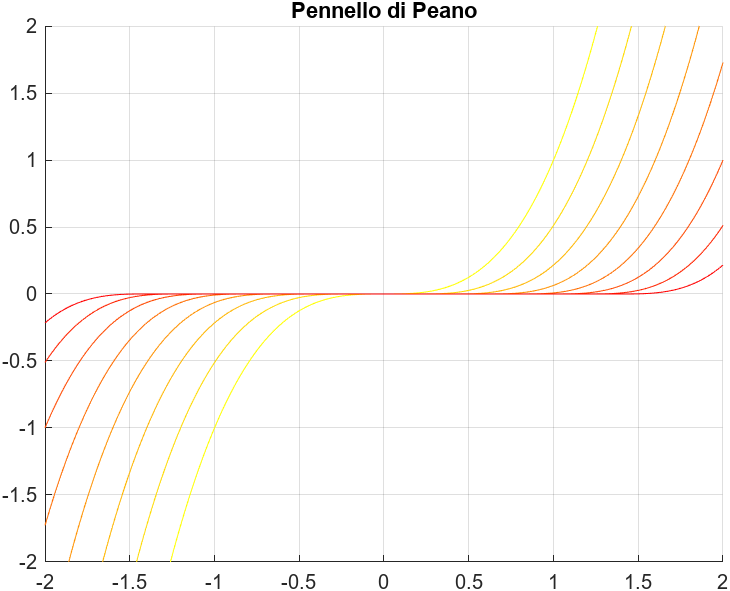
\includegraphics[width=0.31\textwidth]{Capitoli/Capitolo8/Pennello di Peano.png}
\end{figure}
\end{example}
È altresì possibile stabilire una condizione sufficiente per l'esistenza e unicità locale di un problema di Cauchy. Prima però bisogna definire il concetto di lipschitzianità locale (\ref{Def: Funzione lipschitziana}).
\begin{definition}
    Si dice che una funzione $G: A\subseteq \R^{n+1} \to \R^n$ con $A$ aperto è \textbf{localmente Lipschitziana} nell'insieme $A$ in $y$ uniformemente rispetto a $x$ se in ogni compatto $K \subset A$ esiste una costante di Lipschitz $L_K$ tale che
    \begin{equation}
        \forall\ (x, y_1), (x, y_2) \in K \ \text{si ha che}\ |G(x, y_1)-G(x, y_2)| \leq L_K |y_1-y_2|
    \end{equation}
\end{definition}
\begin{theorem}[Teorema di Cauchy di esistenza e unicità locale] \label{Teo: Esistenza e unicità locale}
    Siano $A \subseteq \R^{n+1}$ aperto e $G:A \to \R^n$ continua, localmente Lipschitziana in $Y$ e uniformemente rispetto a $x$ in $B_\delta(x_0, y_0) \subset A$. Sia poi $(x_0, Y_0) \in A$. Allora esiste $\delta>0$ tale che il problema di Cauchy
    \begin{equation}
        (P): \begin{cases}
            Y'=G(x, Y)\\
            Y(x_0)=Y_0
        \end{cases}
    \end{equation}
    ammetta un'unica soluzione locale $\overline{Y}$ per $x \in [x_0-\delta, x_0+\delta]$
\end{theorem}
\begin{proof}
Siano $a, b>0$ tali che si possa definire $R \subseteq A$ come
\begin{equation}
    R= \{(x,y) \mid |x-x_0|\leq a, |y-y_0| \leq b \}
\end{equation}
Siano poi $L>0$ la costante di Lipschitz di $G$ su $R$ e 
\begin{equation}
M=\max\limits_{R}{|G(x, y)|} \qquad 0<\delta<\min\left\{a, \frac{b}{M}, \frac{1}{L}\right\}
\end{equation}
Dopodiché, definito $B$ come
\begin{equation}
    B=\{y \in C^0([x_0-\delta, x_0+\delta]) \mid d_\infty(y, y_0) \leq b\} \subset (C^0([x_0-\delta, x_0+\delta]), d_\infty)
\end{equation}
si mostri che esso è chiuso ($\Rightarrow$ $B$ completo per \ref{Teo: Sottospazio chiuso di un completo è completo}).
Perciò, si consideri una successione $\{y_k\}_k \subset B$ tale che $y_k \to \overline{y}$ rispetto a $d_\infty$. Affinché $B$ sia completo, occorre che $\overline{y} \in B$, cioè $d_\infty(\overline{y},y_0)\leq b$, dunque
\begin{equation}
    d_\infty(\overline{y},y_0) \leq d_\infty(\overline{y},y_k)+ d_\infty(y_k,y_0) \leq d_\infty(\overline{y},y_k) +b
\end{equation}
Allora, passando al limite per $k \to +\infty$ si ha che
\begin{equation}
    d_\infty(\overline{y},y_0) \leq \lim_{k \to +\infty}{d_\infty(\overline{y},y_k) +b}= 0+b= b
\end{equation}
cioè $\overline{y} \in B$, quindi $(B, d_\infty)$ è uno spazio metrico completo.\\
A questo punto, si definisca la mappa $H$
\begin{equation}
    \begin{aligned}
        H: B &\to B\\
        y &\mapsto z:=H(y)
    \end{aligned}
\end{equation}
con
\begin{equation}
    z(x)=y_0+ \int\limits_{x_0}^{x}{G(s, y(s))}\,ds
\end{equation}
Si verifichi che $H$ sia ben definita, cioè che $H(y)$ è continua e che, se $y \in B$, allora $H(y)=z \in B$. Chiaramente $z \in C^0([x_0-\delta, x_0+\delta])$. Inoltre,
\begin{equation}
    |z(x)-y_0|=\left|\int\limits_{x_0}^{x}{G(s, y(s))}\,ds\right| \leq
\int\limits_{x_0}^{x}\left|{G(s, y(s))}\right|\,ds
\end{equation}
Poiché $y \in B$, per ogni $s$ si ha $|y(s)-y_0|\leq b$. Dalla definizione di $\delta$ si ricava che $|s-x_0|<\delta<a$. Perciò $(s, y(s)) \in R$. In particolare, vale anche che $G(s, y(s)) \leq M$. Per definizione di $\delta$, allora,
\begin{equation}
    |z(x)-y_0|\leq M|x-x_0|\leq M\delta \leq b \qquad \forall\ x \in [x_0-\delta, x_0+\delta]
\end{equation}
cioè $H(y) \in B$.\\
Si mostri poi che $H$ è una contrazione. Siano $y_1, y_2 \in B$.
\begin{equation}
\begin{aligned}
    d_\infty(H(y_1), H(y_2))&= \sup_{x \in [x_0-\delta, x_0+\delta]}{|H(y_1)(x)-H(y_2)(x)|}=\\
    &=\sup_{x \in [x_0-\delta, x_0+\delta]}\left|{\int\limits_{x_0}^{x}{\left[G(s,y_1(s))-G(s, y_2(s))\right]}}\,ds\right| \leq \\
    &\leq \sup_{x \in [x_0-\delta, x_0+\delta]}{\int\limits_{x_0}^{x}{\left|G(s,y_1(s))-G(s, y_2(s))\right|}}\,ds \leq\\
    &\leq L\,  \sup_{x \in [x_0-\delta, x_0+\delta]}{\int\limits_{x_0}^{x}{\left|y_1(s)-y_2(s)\right|}}\,ds\leq\\
    &\leq L \,d_\infty(y_1, y_2)\, |x-x_0| \\
    &\leq L\, \delta\, d_\infty(y_1, y_2) \leq \gamma\, d_\infty(y_1,y_2)
\end{aligned}
\end{equation}
dove $\gamma<1$ poiché $\delta<\tfrac{1}{L}$. Dunque $H$ è una contrazione e, per il teorema delle contrazioni \eqref{Teo: delle contrazioni}, esiste un solo punto fisso $y$ tale che
\begin{equation}
    y=H(y)=z= y_0+ \int\limits_{x_0}^{x}{G(s, y(s))}\,ds
\end{equation}
che risolve il problema di Cauchy per il lemma \ref{Lemma: Formulazione integrale del problema di Cauchy}.
\end{proof}
\begin{oss}
    Si noti che una funzione $C^1(A)$ è ivi localmente Lipschitziana, perciò  è sufficiente la regolarità del secondo membro per poter applicare il teorema di Cauchy.
\end{oss}
\begin{example}
    Si riprenda il problema di prima ma si modifichi la condizione iniziale.
    \begin{equation*}
        P: \begin{cases}
        y'=3y^{\frac{2}{3}}\\
        y(0)=3
    \end{cases}
    \end{equation*}
    In questo caso la funzione è $C^\infty(B_\delta(0,3))$, dunque vale il teorema di Cauchy e la soluzione è unica.
\end{example}
\begin{definition} \label{Prolungamento}
    Sia $y(x)$ una soluzione dell'equazione $(E):\ y'=f(x,y)$ definita su $(a,b)$. Si dice che $y_1$ è un \textbf{prolungamento} di $y$ se $y_1(x)$ è una soluzione di $(E)$, è definita su $(a_1, b_1) \supset (a,b)$ e coincide con $y$ in $(a,b)$.\\
    Inoltre, un prolungamento $y_1(x)$ di $y(x)$ si dice \textbf{massimale} se per ogni prolungamento $y_2(x)$ di $y(x)$ definito su $(a_2, b_2)$ si ha che $(a_2, b_2) \subset (a_1, b_1)$.
\end{definition}
\begin{oss}
Data tale definizione, può aver senso ragionare sull'unicità del prolungamento. Perciò, ci si ponga nelle ipotesi del teorema di esistenza e unicità locale. Dopodiché siano $y_1,\ y_2 : (a,b) \to \R$ soluzioni tali che $y_1(x_0)=y_2(x_0)$ e si mostri che non esiste $x_1 \in (a,b)$ tale che $y_1(x_1) \neq y_2(x_1)$. Difatti, se $y_1 \not\equiv y_2$ su $(a,b)$, si avrebbe un punto $x^*$ tale che $y_1(x) \neq y_2(x)$ per $x>x^*$, ma allora
\begin{equation}
    \begin{cases}    
    y'=f(x,y)\\
    y(x_1)=y_1(x_1)=y_2(x_1)
    \end{cases}
\end{equation}
non avrebbe un'unica soluzione locale, contraddicendo così il teorema.\\
In sintesi, dunque, è ragionevole prolungare una soluzione locale di un problema di Cauchy a patto di mantenerne invariata l'unicità.
\end{oss}
Ragionando sul fatto che il teorema garantisca l'esistenza della soluzione in un intorno del punto $x_0$, si può notare che risolvendo il problema agli estremi dell'intorno, la soluzione sarà definita in un intorno dei medesimi, dando così un prolungamento di $y(x)$, con $y(x)$ soluzione. 
\begin{theorem}
    Sotto le ipotesi del teorema di esistenza e unicità locale, la soluzione $y(x)$ ammette sempre un prolungamento massimale.
\end{theorem}
\begin{definition}
    L'intervallo di definizione del prolungamento massimale si dice \textbf{intervallo massimale} di esistenza della soluzione.
\end{definition}
\begin{oss}
    Sia $I_m=(\alpha, \beta)$ l'intervallo massimale di esistenza di una soluzione. Allora, sicuramente per $x \to \beta^-$ non può succedere che 
        \begin{equation}
            \lim_{x \to \beta^-}{y(x)}= \ell \in \R \qquad (\beta, \ell) \in A
        \end{equation}
        poiché se così fosse si potrebbe estendere ulteriormente l'intervallo, ma esso è massimale, e si ha dunque un assurdo.
        Quindi può accadere che
        \begin{itemize}
            \item Esista $\lim\limits_{x \to \beta^-}{y(x)}= \ell \in \R$
            con $(\beta, \ell) \in \partial A$.
            \item Esista $\lim\limits_{x \to \beta^-}{y(x)}= \pm \infty$
            cioè che si abbia un \textit{blow-up} della soluzione.
            \item Non esista $\lim\limits_{x \to \beta^-}{y(x)}$
                cioè la funzione ha delle "oscillazioni" che si avvicinano a $\partial A$.
            \end{itemize}
\end{oss}
Infine, sotto opportune condizioni, è possibile formulare un teorema di esistenza e unicità globale della soluzione.
\begin{theorem}[Teorema di esistenza e unicità globale] \label{Teo: Esistenza e unicità globale}
    Sia $G: (a, b) \times \R^n \to \R^n$ continua e localmente Lipschitziana in $Y$, uniformemente in $x$ in tutto $(a, b) \times \R^n$. Esistano inoltre $h,k \geq 0$ tali che 
    \begin{equation} \label{Eq: Crescità sublineare}
        \left|G(x, Y)\right| \leq h+ k|y|
    \qquad \forall\ (x, Y) \in (a,b) \times \R^n
    \end{equation}
    Allora per ogni $(x_0, Y_0) \in (a,b) \times \R^n$ l'unica soluzione di 
    \begin{equation}
        (P): \begin{cases}
       Y'=G(x, Y)\\
       Y(x_0)=Y_0
       \end{cases}
    \end{equation}
    è prolungabile su tutto $(a, b)$.
\end{theorem}
\section{Equazioni differenziali ordinarie scalari del primo ordine}
Si passi ora allo studio di vari metodi risolutivi per \odes del primo ordine. 
\begin{definition}
    L'insieme di tutte le soluzioni di una \ode o di un sistema è detto \textbf{integrale generale}. Al contrario, ogni singola soluzione è detta \textbf{integrale particolare}.
\end{definition}
\subsection{Equazioni lineari del primo ordine}
Rientrano in questa categoria le equazioni della forma
\begin{equation} \label{Eq: Equazione lineare del primo ordine}
    y'+ a(x) y = g(x)
\end{equation}
con $a,f: I \to \R$ entrambe almeno di classe $C^0(I)$.\\
\begin{definition}
    Un'equazione lineare del primo ordine si dice \textbf{omogenea} se $f \equiv 0$. Altrimenti, si dice \textbf{completa}.
\end{definition}
\begin{theorem} \label{Teo: Integrale generale delle ode lineare del primo ordine}
    Tutte le soluzioni dell'equazione \eqref{Eq: Equazione lineare del primo ordine} sono date da
    \begin{equation}
        y(x)=e^{-A(x)}\left(C+ \int{e^{A(x)}g(x)}\,dx\right)
    \end{equation}
    con $A(x)$ primitiva di $a(x)$ e $C \in \R$ costante.
\end{theorem}
\begin{proof} 
Si provi a ricondurre il primo membro  dell'equazione 
\begin{equation}
    y'+ a(x) y = g(x)
\end{equation}
ad una derivata di prodotto. Per fare ciò, occorre moltiplicare ambo i membri per $e^{A(x) \neq 0}$ in modo da avere
\begin{equation}
    e^{A(x)}(y'+a(x)y)= e^{A(x)}g(x)
\end{equation}
che a primo membro è la derivata di $z(x):=\left(e^{A(x)}y \right)$. Quindi
\begin{equation}
    z'(x)= e^{A(x)}g(x) \iff z(x)=\int e^{A(x)}g(x)\,dx
\end{equation}
Dunque, detta $B(x)$ primitiva di $e^{A(x)}g(x)$, si ha
\begin{equation}
 z(x)= B(x)+C= e^{A(x)}y(x)
 \end{equation}
 e, esplicitando $y(x)$,
 \begin{equation}
    y(x)= B(x) e^{-A(x)} + C{e^{-A(x)}} = e^{-A(x)}\left( C + \int e^{A(x)}g(x)\,dx \right)
 \end{equation}
\end{proof}
\begin{oss}    
Si può notare che tale integrale generale è dato dalla somma di una soluzione particolare e dell'integrale generale dell'equazione omogenea. La soluzione può pertanto essere vista come
\begin{equation}
    y=y_0+ y_p
\end{equation}
dove
\begin{equation}
    y_0= C\, e^{-A(x)} \qquad y_p= \int C\, e^{A(x)}g(x)\,dx
\end{equation}
\end{oss}
\subsubsection{Equazioni di Bernoulli}
Rientrano in questa categoria le equazioni della forma
\begin{equation} \label{Eq: Equazione di Bernoulli}
    y'=a(x)y+ b(x)y^{\alpha}
\end{equation}
con $\alpha \neq 0, 1$, $a, b: I \to \R$, $a,b \in C^0(I)$. Si ipotizzi di voler trovare le $y$ positive.
Si divida per $y^\alpha$.
\begin{equation}
    \frac{y'}{y^\alpha}=a(x)y^{1-\alpha}+ b(x)
\end{equation}
A questo punto, definita
\begin{equation}
    z(x):= \left(y(x)\right)^{1-\alpha}
\end{equation}
si ha che
\begin{equation}
    z'(x)=(1-\alpha)\, y^{-\alpha}\,y'=(1-\alpha)\,y^{-\alpha}\left( a(x)y+ b(x)y^{\alpha}\right)
\end{equation}
cioè
\begin{equation}
    z'(x)=(1-\alpha)\,a(x)\,y^{1-\alpha}+ (1-\alpha)\, b(x) = z'(x)=a(x)\,z+b(x)
\end{equation}
che è lineare in $z$. Dunque, la si può risolvere come previsto dal teorema \eqref{Teo: Integrale generale delle ode lineare del primo ordine}, ricavandone la soluzione $y$ per sostituzione.
\subsection{Equazioni a variabili separabili}
Rientrano in questa categoria le equazioni della forma
\begin{equation} \label{Eq: Equazione a variabili separabili}
    y'=a(x)b(y) 
\end{equation}
con $a:I \to \R,\ b: J \to \R,\ a \in C^0(I),\ b \in C^0(J)$.\\
In particolare, considerando il problema di Cauchy associato a tale equazione, si può osservare che se $a(x)$ è continua in $\U(x_0)$ e $b(y)$ è continua in $\U(y_0)$, allora $a(x)b(y)$ è continua in $B_\delta(x_0, y_0)$ e per il teorema di Peano ammette soluzione locale. Rafforzando tale ipotesi e richiedendo $b(y)$ localmente Lipschitziana rispetto a $y$ o di classe $C^1(\U(y_0))$, allora $a(x)b(y)$ è continua e localmente Lipschitziana e per il teorema di Cauchy ha un'unica soluzione locale.\\
La soluzione dell'equazione prevede due passaggi principali.\\
Innanzitutto occorre cercare le soluzioni costanti, ovvero
\begin{equation}
    y(x)=k \qquad k \in \R
\end{equation}
In altre parole, siccome $k$ è una costante, se essa è soluzione allora si ha 
\begin{equation}
    k' = a(x)b(k) = 0 \iff b(k)=0
\end{equation}
Cercare le soluzioni costanti significa, in altre parole, cercare gli zeri di $b(y)$.\\
Dopodiché occorre cercare le altre soluzioni. Ponendo $b(y) \neq 0$ localmente si ha che
\begin{equation}
    \frac{y'(x)}{b(y(x))}=a(x) \iff \int{\frac{y'(x)}{b(y(x))}}\, dx=\int{a(x)}\, dx 
\end{equation}
Imponendo il cambio di variabile $y=y(x),\ dy=y'(x)dx$ e indicando con $A$ una generica primitiva di $a(x)$, si ha che
\begin{equation}
    \int{\frac{y'(x)}{b(y(x))}}\, dx=\int{a(x)}\, dx \iff \int{\frac{1}{b(y)}}\,dy=A(x)+c_1
\end{equation}
Denotando poi con $B$ una primitiva di $\tfrac{1}{b(y)}$ si ha
\begin{equation}
    B(y)+c_2=A(x)+c_1 \iff B(y)=A(x)+c \iff y=B^{-1}(A(x)+c))
\end{equation}
se $B$ è invertibile. Per il teorema di invertibilità locale, $B$ lo è localmente, perciò, sostituendo all'indietro $y=y(x)$ si ha che l'integrale generale di un'equazione a variabili separabili è
\begin{equation} 
    y(x)=B^{-1}(A(x)+c)
\end{equation}
\subsubsection{Equazioni omogenee}
Con equazioni omogenee si intendono tutte le equazioni della forma
\begin{equation}  \label{Eq: Equazione omogenea}
    y'=f\left(\frac{y}{x}\right)
\end{equation}
con $f:I \to \R$, $f \in C^0(I)$.\\
Tali equazioni sono riconducibili a equazioni a variabili separabili. In particolare, si deve definire una nuova incognita
\begin{equation}
    z(x):=\frac{y(x)}{x} 
\end{equation}
Allora,
\begin{equation}
    z'(x)=\frac{y'(x)x-y(x)}{x^2}=\frac{y'(x)}{x}-{y(x)}{x^2}= \frac{f(\tfrac{y}{x}}{x}-\frac{y}{x}\frac{1}{x}=\frac{f(z(x))}{x}-\frac{z(x)}{x}
\end{equation}
e quindi
\begin{equation}
    z'=\frac{1}{x}\left(f(z)-z\right)
\end{equation}
Risolvendo quindi tale equazione a variabili separabili e sostituendo in modo da esplicitare $y$ si ha la soluzione dell'equazione di partenza \eqref{Eq: Equazione omogenea}.
\subsubsection{Equazioni riconducibili ad autonome}
Rientrano in tale categoria le equazioni della forma
\begin{equation} \label{Eq: Equazione riconducibile ad autonoma}
    y'= g(ax+by)
\end{equation}
con $g:I \to \R,\ a,b \in \R,\ b \neq 0,\ g \in C^0(I)$.\\
Si definisca la nuova incognita 
\begin{equation}
    z:=ax+by(x)
\end{equation}
Allora,
\begin{equation}
    z'=a+by'(x) = a+bg(ax+by)=a+bg(z(x))
\end{equation}
cioè
\begin{equation}
    z'=a+bg(z)
\end{equation}
che è un'equazione autonoma. Risolvendo tale equazione come caso particolare di \eqref{Eq: Equazione a variabili separabili} e sostituendo in modo da esplicitare $y$ si ha la soluzione dell'equazione di partenza \eqref{Eq: Equazione riconducibile ad autonoma}.
\subsection{Equazioni esatte}
Rientrano in questa categoria le equazioni del tipo
\begin{equation}
    y'=-\frac{a(x,y)}{b(x,y)}
\end{equation}
con $\omega=a(x,y)dx+b(x,y)dy$ forma differenziale esatta.\\
Per risolvere tale equazione si può procedere informalmente così:
\begin{equation}
    y'=\frac{dy}{dx}=-\frac{a(x,y)}{b(x,y)} \Rightarrow a(x,y)dx+b(x,y)dy=0
\end{equation}
Poiché $\omega$ è esatta, preso un opportuno potenziale $U$, si ha che
\begin{equation}
\omega= a(x,y)dx+b(x,y)dy = dU(x,y)= 0
\end{equation}
e occorre quindi risolvere
\begin{equation}
    dU(x,y)=0 \iff U(x,y)=C \qquad C\in \R
\end{equation}
Le soluzioni allora sono le curve di livello di $U$, definite implicitamente dall'equazione
\begin{equation}
    U(x,y)=C
\end{equation}
\section{Sistemi lineari}
Siano $A(x) \in \mathbb{M}_{n,n}(\R)$ con $x \in I \subseteq \R$ e $B(x) \in \R^n$ con $x \in I$. Allora un sistema differenziale lineare del primo ordine di $n$ equazioni è dato dall'equazione 
\begin{equation}
    Y'=A(x)Y+B(x)
\end{equation}
\begin{definition}
    Un sistema lineare si dice \textbf{omogeneo} se $B(x) \equiv 0$ in $I$, altrimenti si dice \textbf{completo}.
\end{definition}
\begin{definition}
    Un sistema lineare si dice \textbf{autonomo} o \textbf{a coefficienti costanti} se $A(x) \equiv A$ e $B(x) \equiv B$ in $I$.
\end{definition}
Si consideri il caso $n=2$, allora si avrà che
\begin{align}
    &A(x)=\begin{pmatrix}
        a_{11}(x) & a_{12}(x)\\
        a_{21}(x) & a_{22}(x)
    \end{pmatrix}, \qquad a_{ij}: I \to \R,\ i, j=1,2;\\
    &B(x)=\begin{pmatrix}
        B_1(x)\\
        B_2(x)
    \end{pmatrix}, \qquad b_i:I \to \R,\ i=1,2 
\end{align}
In particolare, si dice che $x \mapsto A(x)$ (equivalentemente per $B$) è continua se $x \mapsto a_{ij}$ è continua per ogni $i, j= 1, \dots, n$.\\
Occorre notare che l'insieme delle soluzioni del sistema omogeneo coincide con il nucleo dell'operatore $L:C^1(I; \R^n) \to C^0(I; \R^n)$ a valori in $\R^n$ dato da
    \begin{equation} \label{Eq: Applicazione L}
        L(Y)=Y'-A(x)Y
    \end{equation}
\begin{proposition}
    L'applicazione $L$
    è lineare.
\end{proposition}
\begin{proof}
    Siano $Y_1, Y_2 \in C^1(I; \R^n)$ e $\alpha, \beta \in \R$. Allora
    \begin{equation}
        \begin{aligned}
            L(\alpha Y_1 + \beta Y_2) &= (\alpha Y_1+ \beta Y_2)'- A(x)(\alpha Y_1 + \beta Y_2) =\\
            &= \alpha Y_1'+ \beta Y_2' - A(x) \alpha Y_1 - A(x) \beta Y_2=\\
            &=\alpha(Y_1'-A(x)Y_1)+ \beta (Y_2'-A(x)Y_2)=\\
            &=\alpha L(Y_1)+\beta L(Y_2)
        \end{aligned}
    \end{equation}
\end{proof}
\begin{oss}    
Come conseguenza rilevante si ha il \textbf{principio di sovrapposizione degli effetti}. Infatti, poste $L(Y_1)=B_1$ e $L(Y_2)=B_2$, si può affermare che
$Z:=Y_1+Y_2$ risolve 
\begin{equation}
    Z'(x)=A(x)Z(x)+B(X)
\end{equation}
infatti, si avrebbe che
\begin{equation}
L(Z)=L(Y_1+Y_2)=L(Y_1)+L(Y_2)=B_1+B_2
\end{equation}
\end{oss}
\subsection{Equivalenza tra sistemi differenziali ed equazioni}
Come già mostrato nel lemma \ref{Lemma: Equivalenza equazione-sistema}, esiste un legame tra equazioni e sistemi differenziali. In particolare, data un'equazione differenziale lineare di ordine $n$
\begin{equation}
    y^{(n)}=a_1(x)y^{(n-1)}+a_2(x)y^{(n-2)}+ \dots+a_n(x)y+b(x)
\end{equation}
e definito il vettore $Y=(Y_1, \dots, Y_n)$ di componenti
\begin{equation}
\begin{aligned}
&Y_1:=y\\
&Y_2:=y'\\
&\qquad \vdots\\
&Y_n:=y^{(n-1)}
\end{aligned}
\end{equation}
si può osservare che tale equazione è equivalente ad un sistema lineare del primo ordine $n\times n$ della forma
\begin{equation}
    \begin{cases}
        Y_1'=Y_2\\
        Y_2'=Y_3\\
        \qquad\vdots\\
        Y_{n-1}'=Y_n\\
        Y_n'= a_1(x) Y_n+ a_2(x) Y_{n-1}+ \dots+ a_n(x) Y_1 + b(x)
    \end{cases}
\end{equation}
Tale sistema può essere scritto in forma compatta come \begin{equation}
Y'=A(x)Y+B(x)
\end{equation}
dove
\begin{align}
&A(x)=\begin{pmatrix}
    0 & 1 & 0 & \dots &  0\\
    \vdots & 0 & 1 & \,  &\vdots\\
    \, & \vdots & 0 & \,  &\,\\
    \, & \, & \vdots & \,  &\,\\
    0 & 0 & 0 & \,  & 1\\
    a_n(x) & a_{n-1}(x) & a_{n-2}(x) & \dots & a_n(x)
\end{pmatrix}\\
&B(x)= \begin{pmatrix}
    0\\
    \vdots\\
    0\\
    b(x)
\end{pmatrix}
\end{align}
Fatta tale premessa, si può osservare anche che è ben posto un eventuale problema di Cauchy della forma
\begin{equation}
    (P)=\begin{cases}
        Y'=A(x)Y+B(x)\\
        Y(x_0)=y_0
    \end{cases}
\end{equation}
e che vale
\begin{theorem}[Teorema di esistenza e unicità globale per sistemi differenziali lineari]
    Siano $A(x) \in \mathbb{M}_{n,n}(\R)$ con $x \in I \subseteq \R$, $B(x) \in \R^n$ con $x \in I$ entrambe continue in $I$. Sia poi $(x_0, y_0) \in I \times \R^n$. Allora il problema di Cauchy
    \begin{equation}
    (P)=\begin{cases}
        Y'=A(x)Y+B(x)\\
        Y(x_0)=y_0
    \end{cases}
    \end{equation}
    ha una ed una sola soluzione $Y: I \to \R^n$.
\end{theorem}
\begin{proof}
    Sia $f(x,y): E=I \times \R^n \to \R^n$ aperto tale che $f(x,Y)=A(x)Y+B(x)$. Allora il sistema può essere visto come 
    \begin{equation}
        Y'=f(x, Y)
    \end{equation}
    Tale funzione è continua in $E$, poiché $A(x),\ B(x)$ sono funzioni continue.
    Inoltre è localmente Lipschitziana in $E$ in $Y$ uniformemente rispetto a $x$, infatti, prese $Y_1,\ Y_2 \in E$
    \begin{equation}
    |f(x, Y_1)- f(x, Y_2)|=|A(x)(Y_1-Y_2)|\leq |A(x)||Y_1-Y_2|
    \end{equation}
    Infine ha una crescita al più lineare \eqref{Eq: Crescità sublineare}. 
    \begin{equation}
        |f(x, Y)|=|A(x)Y+B(x)| \leq |A(x)Y|+|B(x)| \leq |A(X)||Y|+|B(x)|
    \end{equation}
    Dunque la tesi discende dal teorema \ref{Teo: Esistenza e unicità globale}.
\end{proof}
In ultima istanza, vale il seguente risultato, cui si era già fatto cenno nel caso delle equazioni lineari del primo ordine.
\begin{theorem}[Teorema di struttura dell'integrale generale di sistemi differenziali lineari del primo ordine di $n$ equazioni] \label{Teo: Struttura dell'integrale generale per i sistemi}
    Siano rispettivamente $(SC)$ e $(SO)$ il sistema completo ed il sistema omogeneo
    \begin{align}
        &(SC):\ Y'=A(x)Y+ B(x)\\
        &(SO):\ Y'=A(x)Y
    \end{align}
    con $A, B$ continue su $I$.\\
    Allora,
    \begin{enumerate}
        \item L'integrale generale di $(SO)$ è un sottospazio vettoriale $n$-dimensionale di $C^1(I; \R^n)$
        \item L'integrale generale di $(SC)$ si ottiene sommando all'integrale generale di $(SO)$ una soluzione particolare di $(SC)$.
    \end{enumerate}
\end{theorem}
\begin{proof}
    Si dimostri il primo fatto.\\
    È già noto che l'integrale generale di $(SO)$ è un sottospazio vettoriale $S \subset C^1(I, \R^n)$, dal momento che esso è il nucleo di $L$ definita come in \eqref{Eq: Applicazione L}. Occorre dimostrare che esso ha dimensione $n$.
    Si consideri la mappa $T: \R^n\to S$ data da
    \begin{equation}
        T(v):=z(x) \qquad \forall v \in \R^n
    \end{equation}
    dove $z=z(x)$ è l'unica soluzione al problema di Cauchy \begin{equation}
        \begin{cases}    
        z'=A(x)z\\
        z(x_0)= v
        \end{cases}
    \end{equation}
    per un $x_0 \in I$ fissato. Per il teorema di esistenza e unicità globale, $T$ è ben definita ed è lineare: infatti
    \begin{equation}
        T(\alpha v_1 + \beta v_2)= \alpha z_1 + \beta z_2 = \alpha T(v_1)+ \beta T(v_2)
    \end{equation}
    poiché vale la sovrapposizione degli effetti.\\
    Inoltre, $T$ è iniettiva e suriettiva grazie al teorema di esistenza e unicità globale. Dunque $T$ è lineare e biunivoca (cioè un isomorfismo) e \begin{equation}
        \dim S = \dim \R^n = n
    \end{equation}
    Ora si passi al secondo punto.\\
    Siano $Y_O$ una soluzione di $(SO)$ e $Y_P$ una soluzione particolare di $(SC)$. Allora,
    \begin{equation}
        Y=Y_O+Y_P
    \end{equation}
    è soluzione di $(SC)$. Viceversa, sia $Y$ una soluzione qualsiasi di $(SC)$. Allora $Y_O=Y-Y_P$ risolve il sistema omogeneo. Perciò, si può caratterizzare l'integrale generale di $(SC)$ come 
    \begin{equation}
        Y=Y_O+Y_P
    \end{equation}
\end{proof} 
\begin{oss}
    La struttura dell'integrale generale dell'equazione \eqref{Eq: Equazione lineare del primo ordine} è in linea con quanto appena mostrato.
\end{oss}
\subsection{Sistemi differenziali omogenei}
Si consideri il sistema
\begin{equation}
    (S):\ Z'= A(x)Z(x)
\end{equation}
e si stabilisca la forma della soluzione generale.\\
Per determinare l'integrale generale del sistema omogeneo occorre, per quanto detto nel teorema \ref{Teo: Struttura dell'integrale generale per i sistemi} trovare $n$ soluzioni linearmente indipendenti.
\begin{definition} \label{Def: Soluzioni linearmente dipendenti/indipendenti}
    Siano $\varphi_1, \dots, \varphi_n$ con $\varphi_i:I \to \R^n$ 
    soluzioni di $(S)$. Si dice che esse sono \textbf{linearmente dipendenti} se 
    \begin{equation}
        \exists\ (c_1, \dots, c_n) \neq (0, \dots, 0)
    \end{equation}
    tale che
    \begin{equation}
        c_1 \varphi_1(x)+ \dots
        +c_n \varphi_n(x) = 0
    \end{equation}
    In caso contrario, tali soluzioni si dicono \textbf{linearmente indipendenti}.
\end{definition}
\begin{definition} \label{Def: Matrice Wronskiana}
    Date $\varphi_1, \dots, \varphi_n$ con $\varphi_i:I \to \R^n$ 
    soluzioni di $(S)$, si dice \textbf{matrice Wronskiana} la matrice
    \begin{equation}
        W(x):= \begin{pmatrix}
        \varphi_1(x)\mid \varphi_2(x)\mid  \dots \mid \varphi_n(x)
        \end{pmatrix}
    \end{equation}
avente le soluzioni $\varphi_i(x)$ come colonne.\\
Il determinante della Wronskiana è poi detto \textbf{Wronskiano}.
\end{definition}
In maniera equivalente, si può dire che le $\varphi_i(x)$ sono linearmente dipendenti se e solo se lo Wronskiano ad esse associato è nullo per ogni $x \in I$.
\begin{proposition} \label{Prop: Wronskiano nullo sse nullo in I}
    Il determinante Wronskiano è nullo in tutto l'intervallo se e solo se è nullo in almeno un punto di esso.
\end{proposition}
\begin{proof}
   Sia $x_0 \in I$ tale che $c_1 \varphi_1(x_0)+ \dots+c_n \varphi_n(x_0) = 0$ per una certa $(c_1, \dots, c_n) \neq (0, \dots, 0)$.
   Allora, posta
   \begin{equation}
       \xi(x):=c_1 \varphi_1(x)+ \dots
        +c_n \varphi_n(x) \qquad \forall x \in I
   \end{equation}
   essa risolve 
   \begin{equation}
       \begin{cases}
           Y'=A(x)\\
           Y(x_0)=0
       \end{cases}
   \end{equation}
   Poiché però anche $\eta\equiv 0$ risolve tale problema di Cauchy, per il teorema di esistenza e unicità si ha che 
   \begin{equation}
       \xi(x)=c_1 \varphi_1(x)+ \dots
        +c_n \varphi_n(x) =\eta(x) \equiv0
   \end{equation}
\end{proof}
Tale risultato vale anche per verificare la lineare indipendenza.
\begin{definition}
    Siano $\varphi_1, \dots, \varphi_n$ con $\varphi_i:I \to \R^n$ 
    soluzioni di $(S)$ linearmente indipendenti. Allora esse formano un \textbf{sistema fondamentale} di soluzioni.
\end{definition}
Un sistema fondamentale rappresenta dunque una base per $\ker L$ con $L$ definita come in \eqref{Eq: Applicazione L}.\\
L'integrale generale di $(S)$ si può in tale scrivere come 
\begin{equation}
    Y(x)= c_1\varphi_1(x)+ \dots+ c_n\varphi_n(x), \qquad (c_1, \dots, c_n) \in \R^n
\end{equation}
o, in forma compatta, 
\begin{equation}
    Y(x)=W(x)C
\end{equation}
dove $W$ è detta \textit{matrice fondamentale} e $C$ è il vettore colonna delle costanti $c_1, \dots, c_n$.\\
\begin{oss}
    Nel caso di una \ode di ordine $n$ omogenea
    \begin{equation}
        z^{(n)}=a_1(x)z^{(n-1)}+ a_2(x)z^{(n-2)}+ \dots + a_n(x)z
    \end{equation}
    la matrice Wronskiana è data da
    \begin{equation}
        W(x)=\begin{pmatrix}
            y_1(x) & y_2(x) & \dots & y_n(x)\\
            y_1'(x) & y_2'(x) & \dots & y_n'(x)\\
            \vdots & \vdots & \, & \vdots\\
            y_1^{(n-1)}(x) & y_2^{(n-1)}(x) & \dots & y_n^{(n-1)}(x)\\
        \end{pmatrix}
    \end{equation}
\end{oss}
\subsubsection{Sistemi omogenei a coefficienti costanti}
Sono i sistemi del tipo
\begin{equation}
    Y'=AY
\end{equation}
con $A \in \mathbb{M}_{n,n}(\R)$.\\
Nello specifico ci si concentrerà sul caso $n=2$ e
\begin{align}    
    &A=\begin{pmatrix}
        a_{11} & a_{12}\\
        a_{21} & a_{22}
    \end{pmatrix} \qquad a_{ij} \in \R \\
    &Y(x)=\begin{pmatrix}
        y_1(x)\\
        y_2(x)
    \end{pmatrix} \qquad y_i:\R \to \R
\end{align}
o, in componenti,
\begin{equation}
    (S): \begin{cases}
        y_1'=a_{11} y_1 + a_{12} y_2\\
        y_2'=a_{21} y_1 + a_{22} y_2
    \end{cases}
\end{equation}
Per determinare esplicitamente l'integrale generale di $(S)$ occorre studiare 3 diversi casi.
\paragraph{$A$ diagonalizzabile con autovalori reali}
Siano $\lambda_1$, $\lambda_2$ gli autovalori e $U$, $V$ gli autovettori rispettivamente associati.\\
Allora si verifichi che
\begin{equation}
   \xi(x):= e^{\lambda_1 x}U \qquad
   \eta(x):= e^{\lambda_2 x}V
\end{equation}
siano due soluzioni di $(S)$ linearmente indipendenti.
Infatti per $\xi$ vale
\begin{equation}
    A\xi(x)=A(e^{\lambda_1 x}U)=e^{\lambda_1 x}AU = e^{\lambda_1 x} \lambda_1 U = \xi'(x)
\end{equation}
e lo stesso si può dire per $Y_2$. Dunque sono entrambi soluzioni del sistema.
Si calcoli poi 
\begin{equation}
    W(X)=\begin{pmatrix}
        \xi(x) \mid \eta(x)
    \end{pmatrix} = \begin{pmatrix}
        e^{\lambda_1 x} U_1 & e^{\lambda_2 x} V_1 \\
        e^{\lambda_1 x} U_2 & e^{\lambda_2 x} V_2
    \end{pmatrix}
\end{equation}
Allora, sfruttando la proposizione \ref{Prop: Wronskiano nullo sse nullo in I}
\begin{equation}
    \det W(0)=\det(U | V) \neq 0
\end{equation}
poiché per ipotesi $U,\ V$ sono autovettori associati ad autovalori distinti.\\
Di conseguenza, $\xi(x),\ \eta(x)$ sono soluzioni di $(S)$ linearmente indipendenti e l'integrale generale è dato da
\begin{equation}
    Y(x)= c_1 e^{\lambda_1 x}U + c_2 e^{\lambda_2 x}V
\end{equation}
\begin{oss}
    Se $A$ dovesse avere due autovalori reali coincidenti $\lambda_1=\lambda_2=\lambda$, poiché ogni $V \in \R^2$ è autovettore, un sistema fondamentale è dato da $\{e^{\lambda x}V_1, e^{\lambda x}V_2\}$ con $V_1,\ V_2$ linearmente indipendenti.
\end{oss}
\paragraph{$A$ diagonalizzabile con autovalori complessi}
$A$ è diagonalizzabile con autovalori complessi coniugati
\begin{equation}
    \lambda_1=\lambda= \alpha+ i\beta, \qquad
    \lambda_2=\overline{\lambda}= \alpha- i\beta \qquad \alpha, \beta \in \R, \beta \neq0
\end{equation}
In questo caso, anche i due autovettori associati sono complessi coniugati
\begin{equation}
    U=a+ib \qquad \overline{U}=a-ib \qquad a, b \in \R^2, b \neq 0
\end{equation}
Esattamente come prima, si può mostrare che $e^{\lambda x}U,\ e^{\overline{\lambda}x}\overline{U}$
sono soluzioni linearmente indipendenti di $(S)$, ma a valori in $\mathbb{C}^2$. Tuttavia, anche
\begin{align}
    &\Re\left(e^{\lambda x}U\right)= \frac{1}{2}e^{\lambda x}U+\frac{1}{2}e^{\overline{\lambda} x}\overline{U} =: \xi(x)\\
    &\Im\left(e^{\lambda x}U\right)= \frac{1}{2i}e^{\lambda x}U-\frac{1}{2i}e^{\overline{\lambda} x}\overline{U} =: \eta(x)
\end{align}
sono due soluzioni linearmente indipendenti di $(S)$ e a valori in $\R^2$.\\
Dunque l'integrale generale è
\begin{equation}
        Y(x)= c_1 \xi(x) + c_2 \eta(x)
\end{equation}
\paragraph{$A$ non diagonalizzabile}
Se $A$ non è diagonalizzabile, essa ha un solo autovalore $\lambda \in \R$ con molteplicità algebrica $m_a(\lambda)=2$ e molteplicità geometrica $m_g(\lambda)=1$. Il suo autovettore associato è $U$.\\
Come prima, si può mostrare che 
\begin{equation}
    \xi(x)=e^{\lambda x}U
\end{equation}
è soluzione di $(S)$. Tuttavia ne serve un'altra. Per fare ciò occorre trovare un \textit{autovettore generalizzato} $V$ associato a $U$ risolvendo
\begin{equation} \label{Eq: Equazione per autovettore generalizzato}
    (A-\lambda I)V=U
\end{equation}
dunque occorre verificare che 
\begin{equation}
    \eta(x):= e^{\lambda x}(V+xU)
\end{equation}
sia soluzione di $(S)$. Da una parte si ha che
\begin{equation}
    A \eta(x)= A(e^{\lambda x}V+e^{\lambda x}xU) = e^{\lambda x}(AV+ xAU)= e^{\lambda x}(\lambda V + U + \lambda x U)
\end{equation}
Dall'altra, 
\begin{equation}
    \left[e^{\lambda x}(V+xU)\right]'= \lambda
    e^{\lambda x}(V+xU) + e^{\lambda x}U = e^{\lambda x}(\lambda V + U + \lambda x U)
\end{equation}
Quindi $\eta(x)$ risolve il sistema. Resta da verificare l'indipendenza di $\xi$ e $\eta$. Dunque 
\begin{equation}
    W(x)= e^{\lambda x} \begin{pmatrix}
        U_1 & V_1 + x U_1\\
        U_2 & V_2 + x U_2
    \end{pmatrix}
\end{equation}
e 
\begin{equation}
    \det W(0) = \det(U | V) \neq 0
\end{equation}
dal momento che se per assurdo $V= \sigma U$, allora dalla \eqref{Eq: Equazione per autovettore generalizzato} si avrebbe $V=0$, che porta all'assurdo dal momento che gli autovettori sono non nulli per propria definizione.\\
Dunque l'integrale generale è 
\begin{equation}
    Y(x)= e^{\lambda x}[(c_1+c_2x)U+ c_2V]
\end{equation}
\subsection{Sistemi del primo ordine completi a coefficienti continui}
Si consideri il sistema differenziale lineare del primo ordine di $n$ equazioni
\begin{equation}
    Y'=A(x)Y+B(x)
\end{equation}
con $y: I \subseteq \R \to \R^n$, $I$ intervallo e $A, B$ continui in $I$.\\
Si calcoli l'integrale generale del sistema attraverso il \textbf{metodo delle costanti arbitrarie}.
Per il teorema \ref{Teo: Struttura dell'integrale generale per i sistemi}, 
\begin{equation}
    Y(x)=Y_O+Y_P
\end{equation}
dove, per quanto già detto, $Y_O$ è soluzione del sistema fondamentale e quindi
\begin{equation}
    Y_O=W(x)c \qquad c \in \R^n
\end{equation}
Si cerchi una $Y_P$ della forma 
\begin{equation}
    Y_P(x)=W(x)c(x) \qquad c:I\to \R^n
\end{equation}
Poiché vale la relazione 
\begin{equation}
    W'(x)=A(x)W(x)
\end{equation}
si ha anche che
\begin{equation}
\begin{aligned}
    Y_P'(x)&=W'(x)c(x)+W(x)c'(x)=\\
    &=A(x)W(x)c(x)+W(x)c'(x)=\\
    &=A(x)Y_P+W(x)c'(x)
\end{aligned}
\end{equation}
Poiché lo Wronskiano è diverso da zero, $W(x)$ è invertibile per ogni $x \in I$. Quindi
\begin{equation}
    W(x)c'(x) =B(x) \iff c'(x)=W^{-1}(x)B(x)
\end{equation}
cioè
\begin{equation}
    c(x)= \int\limits_{x_0}^{x}{W^{-1}(s)B(s)}\, ds \qquad x_0 \in I
\end{equation}
Perciò
\begin{equation}
Y_P(x)=W(x)c(x)=W(x) \int\limits_{x_0}^{x}{W^{-1}(s)B(s)}\, ds
\end{equation}
Infine, l'integrale generale di tale sistema è dato da 
\begin{equation}
    Y(x)=W(x)\left(c+ \int\limits_{x_0}^{x}{W^{-1}(s)B(s)}\, ds\right)
\end{equation}
\section{Equazioni lineari del secondo ordine a coefficienti costanti}
\subsection{Equazioni omogenee}
Una generica \ode del secondo ordine omogenea a coefficienti costanti è un'equazione del tipo
\begin{equation}
    y''=ay'+by
\end{equation}
con $a,b \in \R$.\\
Per quanto già visto, essa può essere riscritta come sistema
\begin{equation}
    Y'=AY
\end{equation}
con 
\begin{align}
    &A=\begin{pmatrix}
        0 & 1\\
        b & a
    \end{pmatrix}\\
    &Y=\begin{pmatrix}
        y\\
        y'
    \end{pmatrix}
\end{align}
Perciò, il suo polinomio caratteristico sarà
\begin{equation}
    P_A(\lambda)=\det(A-\lambda I) = \lambda^2-a\lambda-b
\end{equation}
e gli autovalori $\lambda_1, \lambda_2$ ne sono soluzione. Anche qui, il discorso si sviluppa in tre casi.
\paragraph{Due autovalori reali distinti} In questo caso si hanno due autovalori $\lambda_1,\ \lambda_2 \in \R$ con $\lambda_1\neq \lambda_2$. Al primo è associato l'autovettore $U$ che risolve
\begin{equation}
    (A- \lambda_1 I)U=0
\end{equation}
e in particolare dette $U_1,\ U_2$ le sue componenti si nota che
\begin{equation}
    -\lambda_1 U_1 + U_2 =0 \iff U_2 = \lambda_1 U_1
\end{equation}
Lo stesso vale per $V$ associato a $\lambda_2$. Nello specifico, poiché in entrambi i casi si ha che la seconda componente è $\lambda_i$ volte l'altra, un possibile autovettore è
\begin{equation}
    U=\begin{pmatrix}
        1\\
        \lambda_1
    \end{pmatrix} \qquad
    V=\begin{pmatrix}
        1\\
        \lambda_2
    \end{pmatrix}
\end{equation}
Per quanto visto prima, 
\begin{align}
    &\xi(x)=e^{\lambda_1 x} \begin{pmatrix}
        1\\
        \lambda_1
    \end{pmatrix}=\begin{pmatrix}
        y_1\\
        y_1'
    \end{pmatrix}\\ 
    &\eta(x)= e^{\lambda_2 x} \begin{pmatrix}
        1\\
        \lambda_2
    \end{pmatrix}=\begin{pmatrix}
        y_2\\
        y_2'
        \end{pmatrix}
\end{align}
risolvono il sistema e sono linearmente indipendenti.\\
Dunque l'integrale generale è \begin{equation}
    y(x)=c_1e^{\lambda_1 x} + c_2 e^{\lambda_2 x}
\end{equation}
\paragraph{Due autovalori complessi distinti}
Gli autovalori sono $\lambda_1,\ \lambda_2 \in \mathbb{C}$ con
\begin{equation}
    \lambda_1=\lambda= \alpha+ i\beta, \qquad
    \lambda_2=\overline{\lambda}= \alpha- i\beta \qquad \alpha, \beta \in \R, \beta \neq0
\end{equation}
Come nel caso precedente si può verificare che
\begin{equation}
    U = \begin{pmatrix}
        1\\ 
        \lambda
        \end{pmatrix}
\end{equation}
è un autovettore di $A$ associato a $\lambda$. Inoltre,
\begin{align}
    &\xi(x) = \Re(e^{\lambda x}U)\\
    &\eta(x)= \Im(e^{\lambda x}U)
\end{align}
sono soluzioni linearmente indipendenti del sistema le cui prime componenti sono 
\begin{align}
    y_1(x)=\Re\left(e^{\lambda x}\right) = \Re\left(e^{\alpha x + i \beta x}\right)=e^{\alpha x} \cos(\beta x)\\
    y_2(x)=\Im\left(e^{\lambda x }\right)=\Im\left(e^{\alpha x + i \beta x}\right)=e^{\alpha x} \sin(\beta x)
\end{align}
Dunque, l'integrale generale dell'equazione è
\begin{equation}
    y(x)=e^{\alpha x}[c_1 \cos(\beta
    x) + c_2\sin(\beta x)]
\end{equation}
\paragraph{Due autovalori reali coincidenti}
Si ha un unico autovalore $\lambda \in \R$ con $m_a(\lambda)=2$ e $m_g(\lambda)<2$. Dunque la matrice $A$ non è mai diagonalizzabile. Si può verificare che un autovettore associato è 
\begin{equation}
    U= \begin{pmatrix}
        1\\
        \lambda
    \end{pmatrix}
\end{equation}
Come verificato nel caso 3 della sezione precedente, si può affermare che 
\begin{align}
    &\xi(x)=e^{\lambda
    x}U\\
    &\eta(x)=e^{\lambda x}(V-xU)
\end{align}
sono soluzioni linearmente indipendenti del sistema associato, dove $V$ è l'autovettore generalizzato che risolve 
\begin{equation}
    (A-\lambda I)V=U \iff \begin{pmatrix}
        -\lambda & 1\\
        b & a-\lambda
    \end{pmatrix}
    \begin{pmatrix}
        v_1\\
        v_2
    \end{pmatrix}= \begin{pmatrix}
        1\\
        \lambda
    \end{pmatrix}
\end{equation}
Dal momento che $\lambda= \tfrac{a}{2}$ e $b=-\tfrac{a^2}{4}$ si ha
\begin{equation}
    \begin{pmatrix}
        -\frac{a}{2} & 1\\
        -\frac{a^2}{4} & a-\frac{a}{2}
    \end{pmatrix}
    \begin{pmatrix}
        v_1\\
        v_2
    \end{pmatrix}= \begin{pmatrix}
        1\\
        \frac{a}{2}
        \end{pmatrix}
\end{equation}
e, dalla prima, si ottiene $V_2=1+\tfrac{a}{2}V_1$. Posto $V_1=0$, un autovettore generalizzato è
\begin{equation}
    V=\begin{pmatrix}
        0\\
        1
    \end{pmatrix}
\end{equation}
Perciò, sostituendo $V$ nell'equazione di $\eta(x)$ e scegliendo la prima componente di ciascun autovettore, si ha che l'integrale generale è
\begin{equation}
y(x)= e^{\lambda x}(c_1+c_2 x)    
\end{equation}
\subsection{Equazioni non omogenee}
Si tratta di equazioni del tipo
\begin{equation}
    y'' - ay'-by=f(x)
\end{equation}
dove $f:I \subseteq \R \to \R$ è una funzione continua detta \textbf{forzante}.\\
Dal teorema \ref{Teo: Struttura dell'integrale generale per i sistemi} è noto che l'integrale generale è della forma 
\begin{equation}
    y(x)= y_{O}+ y_{P}
\end{equation}
con $y_{O}$ soluzione dell'equazione omogenea e $y_{P}$ soluzione particolare dell'equazione completa, di cui si dirà di più ora.
\subsubsection{Metodo di somiglianza}
Un metodo risolutivo può essere il cosiddetto \textbf{metodo di somiglianza} che consiste nel cercare una soluzione particolare $y_P$ sulla base della sua somiglianza alla forzante.
\paragraph{Caso 1} La forzante è un polinomio di grado $n$
\begin{equation}
    f(x)=Q_n(x)= q_nx^n+q_{n-1}x^{n-1}+ \dots +q_0
\end{equation}
con $q_n, q_{n-1}, \dots, q_0 \in \R$ coefficienti noti e $q_n \neq 0$.
Allora, preso il polinomio caratteristico
\begin{equation}
    P(\lambda)=\lambda^2 - a\lambda-b
\end{equation}
si ha che
\begin{equation}
    y_P(x)=\begin{cases}
        R_n(x) &\qquad \text{se}\ \lambda=0\ \text{\textbf{non} è radice di}\ P(\lambda)=0\\
        xR_n(x) &\qquad \text{se}\ \lambda=0\ \text{è radice \textbf{semplice} di}\ P(\lambda)=0\\
        x^2R_n(x) &\qquad \text{se}\ \lambda=0\ \text{è radice \textbf{doppia} di}\ P(\lambda)=0\\
    \end{cases}
\end{equation}
con $R_n(x)=a_nx^n+ a_{n-1}x^{n-1}+\dots+a_0$ polinomio di grado $n$ i cui coefficienti vanno determinati in modo tale che $y_P$ risolva l'equazione completa.
\paragraph{Caso 2} La forzante è una funzione esponenziale
\begin{equation}
    f(x)= A e^{\alpha x}
\end{equation}
con $A, \alpha \in \R$. Allora, 
\begin{equation}
    y_P(x)= \begin{cases}
        C e^{\alpha x} &\qquad \text{se}\ \lambda=\alpha\ \text{\textbf{non} è radice di}\ P(\lambda)=0\\
        C xe^{\alpha x} &\qquad \text{se}\ \lambda=\alpha\ \text{è radice \textbf{semplice} di}\ P(\lambda)=0\\
        Cx^2 e^{\alpha x} &\qquad \text{se}\ \lambda=\alpha\ \text{è radice \textbf{doppia} di}\ P(\lambda)=0\\
    \end{cases}
\end{equation}
con $C \in \R$ da determinare in modo che $y_P$ risolva l'equazione completa.
\paragraph{Caso 3} La forzante è il prodotto di un polinomio di grado $n$ e una funzione esponenziale
\begin{equation}
    f(x)=Q_n(x) e^{\alpha x}
\end{equation}
con $Q_n(x)$ come nel caso 1. Allora
\begin{equation}
    y_P(x)= \begin{cases}
        R_n(x) e^{\alpha x} &\qquad \text{se}\ \lambda=\alpha\ \text{\textbf{non} è radice di}\ P(\lambda)=0\\
        x R_n(x)e^{\alpha x} &\qquad \text{se}\ \lambda=\alpha\ \text{è radice \textbf{semplice} di}\ P(\lambda)=0\\
        x^2 R_n(x) e^{\alpha x} &\qquad \text{se}\ \lambda=\alpha\ \text{è radice \textbf{doppia} di}\ P(\lambda)=0\\
    \end{cases}
\end{equation}
con $R_n(x)$ come nel caso 1 da determinare.
\paragraph{Caso 4} La forzante è il prodotto di una funzione esponenziale ed una combinazione di funzioni trigonometriche
\begin{equation}
    f(x)=e^{\alpha x} \{A \sin(\beta x)+ C \cos(\beta x)\}
\end{equation}
con $A,\ C,\ \alpha,\ \beta \in \R$. Allora
\begin{equation}
    y_P(x)= \begin{cases}
        e^{\alpha x}\{k \cos(\beta x) + h \sin(\beta x)\} &\quad \text{se}\ \lambda=\alpha+i\beta\ \text{\textbf{non} è radice di}\ P(\lambda)=0\\
        xe^{\alpha x}\{k \cos(\beta x) + h \sin(\beta x)\} &\quad \text{se}\ \lambda=\alpha+i\beta\ \text{è radice \textbf{semplice} di}\ P(\lambda)=0\\ 
    \end{cases}
\end{equation}
\paragraph{Caso 5} La forzante è somma di funzioni come quelle appena mostrate. Vale il principio di sovrapposizione degli effetti, perciò si possono studiare singolarmente le varie forzanti, per poi sommare le diverse soluzioni particolari ottenute.
\section{Studi qualitativi}
Sia (P) un problema di Cauchy per una \ode del primo ordine
\begin{equation}
    (P): \begin{cases}
        y'=f(x,y)\\
        y(x_0)=y_0
    \end{cases}
\end{equation}
con $f: A \subseteq \R^2 \to \R$, $(x_0, y_0) \in A$, $y:I_m \subseteq \R \to \R$.\\
Talvolta può essere necessario studiare alcune proprietà della soluzione $y(x)$ e del suo grafico senza però risolverla esplicitamente.
Per fare ciò si può seguire una precisa procedura.
\begin{enumerate}
    \item Verificare la validità dei teoremi di \textit{esistenza} e \textit{unicità} locale (\ref{Teo: Esistenza e unicità locale}) e globale (\ref{Teo: Esistenza e unicità globale}).\\
    Qualora le ipotesi globali non fossero soddisfatte, occorre ridurre l'intervallo massimale $I_m$.
    \item Trovare le regioni di \textit{monotonia}
    \begin{equation}
        y'\geq 0 \iff f(x,y) \geq 0
    \end{equation}
    \item Eventualmente trovare le regioni di \textit{convessità}
    \begin{equation}
        y'' \geq 0 \iff [f(x,y(x))]' = \frac{\partial f}{\partial x}(x,y(x))+ f(x,y(x)) \frac{\partial f}{\partial y}(x,y(x)) \geq 0
    \end{equation}
    \item Determinare esplicitamente $I_m$.
    \item Cercare eventuali \textit{soluzioni costanti}.
    \item Studiare eventuali \textit{asintoti}.
    \item Studiare eventuali \textit{simmetrie}.
\end{enumerate}
A tale scopo valgono due risultati.
\begin{theorem}[Confronto per equazioni differenziali ordinarie]
    Siano $I,J \subseteq \R$ due intervalli, $f:I\times J \to \R$ continua, localmente Lipschitziana in $y$, uniformemente rispetto a $x$ e $x_0 \in I$. Esistano $U,V: I \to J$ derivabili tali che $\forall\ x \in I$
    \begin{equation}
        \begin{aligned}
            U'(x) &\leq f(x, U(x))\\
            V'(x) & \geq f(x, V(x)
        \end{aligned}
    \end{equation}
    Allora,
    \begin{equation}
     U(x_0) \leq V(x_0) \Rightarrow U(x) \leq V(x) \qquad \forall\ x \geq x_0,\ x \in I \end{equation}
    oppure
    \begin{equation}
    U(x_0) \geq V(x_0) \Rightarrow U(x) \geq V(x) \qquad \forall\ x \leq x_0,\ x \in I \end{equation}
\end{theorem}
\begin{theorem}[Criterio dell'asintoto]
    Sia $U:[a, +\infty]\to \R$ derivabile. Se esistono
    \begin{equation}
        \ell:=\lim_{x \to \infty}{U(x)} \in \R
    \end{equation}
    e 
    \begin{equation}
        m:=\lim_{x \to \infty}{U'(x)} \in [-\infty, +\infty]
    \end{equation}
    allora necessariamente $m=0$.
\end{theorem}
\subsection{Equazioni autonome scalari}
Rientrano in questa categoria le equazioni della forma
\begin{equation}
    y'=f(y)
\end{equation}
con $f \in C^1$.
Si può notare che tali equazioni godono della proprietà di invarianza nel tempo. Infatti, se $y(x)$ risolve $y'=f(y)$, allora anche $z(x)=y(x+t)$, $t\in \R$ risolve $y'=f(x)$.
\begin{equation}
    z'(x)=y'(x+t) \overset{s=x+t}{=}y'(s)
\end{equation}
che risolve l'equazione, dunque anche $z(x)$ è una soluzione dell'equazione.\\
A causa di questa proprietà, può essere utile rappresentare la soluzione in un diagramma di fase in cui si indicano con dei punti le soluzioni costanti (o \textbf{equilibri}) e con delle frecce gli intervalli di monotonia. Si tratta tuttavia di uno strumento qualitativo che non indaga in maniera esplicita convessità ed eventuali asintoti verticali o obliqui.\cleardoublepage
\end{document}